\documentclass[twoside]{book}

% Packages required by doxygen
\usepackage{fixltx2e}
\usepackage{calc}
\usepackage{doxygen}
\usepackage[export]{adjustbox} % also loads graphicx
\usepackage{graphicx}
\usepackage[utf8]{inputenc}
\usepackage{makeidx}
\usepackage{multicol}
\usepackage{multirow}
\PassOptionsToPackage{warn}{textcomp}
\usepackage{textcomp}
\usepackage[nointegrals]{wasysym}
\usepackage[table]{xcolor}

% NLS support packages
platex
% Font selection
\usepackage[T1]{fontenc}
\usepackage[scaled=.90]{helvet}
\usepackage{courier}
\usepackage{amssymb}
\usepackage{sectsty}
\renewcommand{\familydefault}{\sfdefault}
\allsectionsfont{%
  \fontseries{bc}\selectfont%
  \color{darkgray}%
}
\renewcommand{\DoxyLabelFont}{%
  \fontseries{bc}\selectfont%
  \color{darkgray}%
}
\newcommand{\+}{\discretionary{\mbox{\scriptsize$\hookleftarrow$}}{}{}}

% Page & text layout
\usepackage{geometry}
\geometry{%
  a4paper,%
  top=2.5cm,%
  bottom=2.5cm,%
  left=2.5cm,%
  right=2.5cm%
}
\tolerance=750
\hfuzz=15pt
\hbadness=750
\setlength{\emergencystretch}{15pt}
\setlength{\parindent}{0cm}
\setlength{\parskip}{3ex plus 2ex minus 2ex}
\makeatletter
\renewcommand{\paragraph}{%
  \@startsection{paragraph}{4}{0ex}{-1.0ex}{1.0ex}{%
    \normalfont\normalsize\bfseries\SS@parafont%
  }%
}
\renewcommand{\subparagraph}{%
  \@startsection{subparagraph}{5}{0ex}{-1.0ex}{1.0ex}{%
    \normalfont\normalsize\bfseries\SS@subparafont%
  }%
}
\makeatother

% Headers & footers
\usepackage{fancyhdr}
\pagestyle{fancyplain}
\fancyhead[LE]{\fancyplain{}{\bfseries\thepage}}
\fancyhead[CE]{\fancyplain{}{}}
\fancyhead[RE]{\fancyplain{}{\bfseries\leftmark}}
\fancyhead[LO]{\fancyplain{}{\bfseries\rightmark}}
\fancyhead[CO]{\fancyplain{}{}}
\fancyhead[RO]{\fancyplain{}{\bfseries\thepage}}
\fancyfoot[LE]{\fancyplain{}{}}
\fancyfoot[CE]{\fancyplain{}{}}
\fancyfoot[RE]{\fancyplain{}{\bfseries\scriptsize Generated by Doxygen }}
\fancyfoot[LO]{\fancyplain{}{\bfseries\scriptsize Generated by Doxygen }}
\fancyfoot[CO]{\fancyplain{}{}}
\fancyfoot[RO]{\fancyplain{}{}}
\renewcommand{\footrulewidth}{0.4pt}
\renewcommand{\chaptermark}[1]{%
  \markboth{#1}{}%
}
\renewcommand{\sectionmark}[1]{%
  \markright{\thesection\ #1}%
}

% Indices & bibliography
\usepackage{natbib}
\usepackage[titles]{tocloft}
\setcounter{tocdepth}{3}
\setcounter{secnumdepth}{5}
\makeindex

% Hyperlinks (required, but should be loaded last)
\usepackage{ifpdf}
\ifpdf
  \usepackage[pdftex,pagebackref=true]{hyperref}
\else
  \usepackage[ps2pdf,pagebackref=true]{hyperref}
\fi
\hypersetup{%
  colorlinks=true,%
  linkcolor=blue,%
  citecolor=blue,%
  unicode%
}

% Custom commands
\newcommand{\clearemptydoublepage}{%
  \newpage{\pagestyle{empty}\cleardoublepage}%
}

\usepackage{caption}
\captionsetup{labelsep=space,justification=centering,font={bf},singlelinecheck=off,skip=4pt,position=top}

%===== C O N T E N T S =====

\begin{document}

% Titlepage & ToC
\hypersetup{pageanchor=false,
             bookmarksnumbered=true,
             pdfencoding=unicode
            }
\pagenumbering{alph}
\begin{titlepage}
\vspace*{7cm}
\begin{center}%
{\Large Reversi\+Form \\[1ex]\large 1.\+0.\+0 }\\
\vspace*{1cm}
{\large Generated by Doxygen 1.8.13}\\
\end{center}
\end{titlepage}
\clearemptydoublepage
\pagenumbering{roman}
\tableofcontents
\clearemptydoublepage
\pagenumbering{arabic}
\hypersetup{pageanchor=true}

%--- Begin generated contents ---
\chapter{Namespace Index}
\section{Packages}
Here are the packages with brief descriptions (if available)\+:\begin{DoxyCompactList}
\item\contentsline{section}{\hyperlink{namespace_reversi_form}{Reversi\+Form} }{\pageref{namespace_reversi_form}}{}
\item\contentsline{section}{\hyperlink{namespace_reversi_form_1_1_properties}{Reversi\+Form.\+Properties} }{\pageref{namespace_reversi_form_1_1_properties}}{}
\end{DoxyCompactList}

\chapter{Hierarchical Index}
\section{Class Hierarchy}
This inheritance list is sorted roughly, but not completely, alphabetically\+:\begin{DoxyCompactList}
\item Form\begin{DoxyCompactList}
\item \contentsline{section}{Reversi4color\+Form.\+Reversi}{\pageref{class_reversi4color_form_1_1_reversi}}{}
\item \contentsline{section}{Reversi4color\+Form.\+Setting\+Form}{\pageref{class_reversi4color_form_1_1_setting_form}}{}
\end{DoxyCompactList}
\item \contentsline{section}{Form\+Main}{\pageref{class_form_main}}{}
\item \contentsline{section}{Reversi4color\+Form.\+Hsl\+Color}{\pageref{class_reversi4color_form_1_1_hsl_color}}{}
\item \contentsline{section}{Reversi4color\+Form.\+My\+Reversi}{\pageref{class_reversi4color_form_1_1_my_reversi}}{}
\item \contentsline{section}{Reversi4color\+Form.\+Program}{\pageref{class_reversi4color_form_1_1_program}}{}
\item \contentsline{section}{Reversi4color\+Form.\+Reversi\+Anz}{\pageref{class_reversi4color_form_1_1_reversi_anz}}{}
\item \contentsline{section}{Reversi4color\+Form.\+Reversi\+Const}{\pageref{class_reversi4color_form_1_1_reversi_const}}{}
\item \contentsline{section}{Reversi4color\+Form.\+Reversi\+History}{\pageref{class_reversi4color_form_1_1_reversi_history}}{}
\item \contentsline{section}{Reversi4color\+Form.\+Reversi\+Play}{\pageref{class_reversi4color_form_1_1_reversi_play}}{}
\item \contentsline{section}{Reversi4color\+Form.\+Reversi\+Point}{\pageref{class_reversi4color_form_1_1_reversi_point}}{}
\item \contentsline{section}{Reversi4color\+Form.\+Reversi\+Setting}{\pageref{class_reversi4color_form_1_1_reversi_setting}}{}
\end{DoxyCompactList}

\chapter{Class Index}
\section{Class List}
Here are the classes, structs, unions and interfaces with brief descriptions\+:\begin{DoxyCompactList}
\item\contentsline{section}{\hyperlink{class_form_main}{Form\+Main} \\*Form\+Mainクラス }{\pageref{class_form_main}}{}
\item\contentsline{section}{\hyperlink{class_reversi4color_form_1_1_hsl_color}{Reversi4color\+Form.\+Hsl\+Color} \\*H\+SL (H\+LS) カラーを表す }{\pageref{class_reversi4color_form_1_1_hsl_color}}{}
\item\contentsline{section}{\hyperlink{class_reversi4color_form_1_1_my_reversi}{Reversi4color\+Form.\+My\+Reversi} \\*リバーシクラス }{\pageref{class_reversi4color_form_1_1_my_reversi}}{}
\item\contentsline{section}{\hyperlink{class_reversi4color_form_1_1_program}{Reversi4color\+Form.\+Program} }{\pageref{class_reversi4color_form_1_1_program}}{}
\item\contentsline{section}{\hyperlink{class_reversi4color_form_1_1_reversi}{Reversi4color\+Form.\+Reversi} }{\pageref{class_reversi4color_form_1_1_reversi}}{}
\item\contentsline{section}{\hyperlink{class_reversi4color_form_1_1_reversi_anz}{Reversi4color\+Form.\+Reversi\+Anz} \\*リバーシ解析クラス }{\pageref{class_reversi4color_form_1_1_reversi_anz}}{}
\item\contentsline{section}{\hyperlink{class_reversi4color_form_1_1_reversi_const}{Reversi4color\+Form.\+Reversi\+Const} \\*アプリ設定クラス }{\pageref{class_reversi4color_form_1_1_reversi_const}}{}
\item\contentsline{section}{\hyperlink{class_reversi4color_form_1_1_reversi_history}{Reversi4color\+Form.\+Reversi\+History} \\*リバーシ履歴クラス }{\pageref{class_reversi4color_form_1_1_reversi_history}}{}
\item\contentsline{section}{\hyperlink{class_reversi4color_form_1_1_reversi_play}{Reversi4color\+Form.\+Reversi\+Play} \\*リバーシプレイクラス }{\pageref{class_reversi4color_form_1_1_reversi_play}}{}
\item\contentsline{section}{\hyperlink{class_reversi4color_form_1_1_reversi_point}{Reversi4color\+Form.\+Reversi\+Point} \\*リバーシポイント }{\pageref{class_reversi4color_form_1_1_reversi_point}}{}
\item\contentsline{section}{\hyperlink{class_reversi4color_form_1_1_reversi_setting}{Reversi4color\+Form.\+Reversi\+Setting} \\*アプリ設定クラス }{\pageref{class_reversi4color_form_1_1_reversi_setting}}{}
\item\contentsline{section}{\hyperlink{class_reversi4color_form_1_1_setting_form}{Reversi4color\+Form.\+Setting\+Form} \\*Setting\+Formクラス }{\pageref{class_reversi4color_form_1_1_setting_form}}{}
\end{DoxyCompactList}

\chapter{File Index}
\section{File List}
Here is a list of all documented files with brief descriptions\+:\begin{DoxyCompactList}
\item\contentsline{section}{\hyperlink{_form_main_8cs}{Form\+Main.\+cs} \\*Form\+Mainクラス }{\pageref{_form_main_8cs}}{}
\item\contentsline{section}{{\bfseries Form\+Main.\+Designer.\+cs} }{\pageref{_form_main_8_designer_8cs}}{}
\item\contentsline{section}{{\bfseries Program.\+cs} }{\pageref{_program_8cs}}{}
\item\contentsline{section}{\hyperlink{_setting_form_8cs}{Setting\+Form.\+cs} \\*Setting\+Formクラス }{\pageref{_setting_form_8cs}}{}
\item\contentsline{section}{{\bfseries Setting\+Form.\+Designer.\+cs} }{\pageref{_setting_form_8_designer_8cs}}{}
\item\contentsline{section}{Model/\hyperlink{_hsl_color_8cs}{Hsl\+Color.\+cs} \\*Hsl\+Colorクラス }{\pageref{_hsl_color_8cs}}{}
\item\contentsline{section}{Model/\hyperlink{_my_reversi_8cs}{My\+Reversi.\+cs} \\*リバーシクラス実装ファイル }{\pageref{_my_reversi_8cs}}{}
\item\contentsline{section}{Model/\hyperlink{_reversi_anz_8cs}{Reversi\+Anz.\+cs} \\*リバーシ解析クラス実装ファイル }{\pageref{_reversi_anz_8cs}}{}
\item\contentsline{section}{Model/\hyperlink{_reversi_const_8cs}{Reversi\+Const.\+cs} \\*アプリ定数クラス }{\pageref{_reversi_const_8cs}}{}
\item\contentsline{section}{Model/\hyperlink{_reversi_history_8cs}{Reversi\+History.\+cs} \\*リバーシ履歴クラス実装ファイル }{\pageref{_reversi_history_8cs}}{}
\item\contentsline{section}{Model/\hyperlink{_reversi_play_8cs}{Reversi\+Play.\+cs} \\*リバーシプレイクラス実装ファイル }{\pageref{_reversi_play_8cs}}{}
\item\contentsline{section}{Model/\hyperlink{_reversi_point_8cs}{Reversi\+Point.\+cs} \\*リバーシポイントクラス実装ファイル }{\pageref{_reversi_point_8cs}}{}
\item\contentsline{section}{Model/\hyperlink{_reversi_setting_8cs}{Reversi\+Setting.\+cs} \\*アプリ設定クラス }{\pageref{_reversi_setting_8cs}}{}
\item\contentsline{section}{obj/\+Debug/{\bfseries Temporary\+Generated\+File\+\_\+036\+C0\+B5\+B-\/1481-\/4323-\/8\+D20-\/8\+F5\+A\+D\+C\+B23\+D92.\+cs} }{\pageref{_debug_2_temporary_generated_file__036_c0_b5_b-1481-4323-8_d20-8_f5_a_d_c_b23_d92_8cs}}{}
\item\contentsline{section}{obj/\+Debug/{\bfseries Temporary\+Generated\+File\+\_\+5937a670-\/0e60-\/4077-\/877b-\/f7221da3dda1.\+cs} }{\pageref{_debug_2_temporary_generated_file__5937a670-0e60-4077-877b-f7221da3dda1_8cs}}{}
\item\contentsline{section}{obj/\+Debug/{\bfseries Temporary\+Generated\+File\+\_\+\+E7\+A71\+F73-\/0\+F8\+D-\/4\+B9\+B-\/\+B56\+E-\/8\+E70\+B10\+B\+C5\+D3.\+cs} }{\pageref{_debug_2_temporary_generated_file___e7_a71_f73-0_f8_d-4_b9_b-_b56_e-8_e70_b10_b_c5_d3_8cs}}{}
\item\contentsline{section}{obj/\+Release/{\bfseries Temporary\+Generated\+File\+\_\+036\+C0\+B5\+B-\/1481-\/4323-\/8\+D20-\/8\+F5\+A\+D\+C\+B23\+D92.\+cs} }{\pageref{_release_2_temporary_generated_file__036_c0_b5_b-1481-4323-8_d20-8_f5_a_d_c_b23_d92_8cs}}{}
\item\contentsline{section}{obj/\+Release/{\bfseries Temporary\+Generated\+File\+\_\+5937a670-\/0e60-\/4077-\/877b-\/f7221da3dda1.\+cs} }{\pageref{_release_2_temporary_generated_file__5937a670-0e60-4077-877b-f7221da3dda1_8cs}}{}
\item\contentsline{section}{obj/\+Release/{\bfseries Temporary\+Generated\+File\+\_\+\+E7\+A71\+F73-\/0\+F8\+D-\/4\+B9\+B-\/\+B56\+E-\/8\+E70\+B10\+B\+C5\+D3.\+cs} }{\pageref{_release_2_temporary_generated_file___e7_a71_f73-0_f8_d-4_b9_b-_b56_e-8_e70_b10_b_c5_d3_8cs}}{}
\item\contentsline{section}{Properties/{\bfseries Assembly\+Info.\+cs} }{\pageref{_assembly_info_8cs}}{}
\item\contentsline{section}{Properties/{\bfseries Resources.\+Designer.\+cs} }{\pageref{_resources_8_designer_8cs}}{}
\item\contentsline{section}{Properties/{\bfseries Settings.\+Designer.\+cs} }{\pageref{_settings_8_designer_8cs}}{}
\end{DoxyCompactList}

\chapter{Namespace Documentation}
\hypertarget{namespace_reversi_form}{}\section{Reversi\+Form Namespace Reference}
\label{namespace_reversi_form}\index{Reversi\+Form@{Reversi\+Form}}
\subsection*{Namespaces}
\begin{DoxyCompactItemize}
\end{DoxyCompactItemize}
\subsection*{Classes}
\begin{DoxyCompactItemize}
\item 
class \hyperlink{class_reversi_form_1_1_hsl_color}{Hsl\+Color}
\begin{DoxyCompactList}\small\item\em H\+SL (H\+LS) カラーを表す \end{DoxyCompactList}\item 
class \hyperlink{class_reversi_form_1_1_my_reversi}{My\+Reversi}
\begin{DoxyCompactList}\small\item\em リバーシクラス \end{DoxyCompactList}\item 
class \hyperlink{class_reversi_form_1_1_program}{Program}
\item 
class \hyperlink{class_reversi_form_1_1_reversi}{Reversi}
\item 
class \hyperlink{class_reversi_form_1_1_reversi_anz}{Reversi\+Anz}
\begin{DoxyCompactList}\small\item\em リバーシ解析クラス \end{DoxyCompactList}\item 
class \hyperlink{class_reversi_form_1_1_reversi_const}{Reversi\+Const}
\begin{DoxyCompactList}\small\item\em アプリ設定クラス \end{DoxyCompactList}\item 
class \hyperlink{class_reversi_form_1_1_reversi_history}{Reversi\+History}
\begin{DoxyCompactList}\small\item\em リバーシ履歴クラス \end{DoxyCompactList}\item 
class \hyperlink{class_reversi_form_1_1_reversi_play}{Reversi\+Play}
\begin{DoxyCompactList}\small\item\em リバーシプレイクラス \end{DoxyCompactList}\item 
class \hyperlink{class_reversi_form_1_1_reversi_point}{Reversi\+Point}
\begin{DoxyCompactList}\small\item\em リバーシポイント \end{DoxyCompactList}\item 
class \hyperlink{class_reversi_form_1_1_reversi_setting}{Reversi\+Setting}
\begin{DoxyCompactList}\small\item\em アプリ設定クラス \end{DoxyCompactList}\item 
class \hyperlink{class_reversi_form_1_1_setting_form}{Setting\+Form}
\begin{DoxyCompactList}\small\item\em Setting\+Formクラス \end{DoxyCompactList}\end{DoxyCompactItemize}

\hypertarget{namespace_reversi_form_1_1_properties}{}\section{Reversi\+Form.\+Properties Namespace Reference}
\label{namespace_reversi_form_1_1_properties}\index{Reversi\+Form.\+Properties@{Reversi\+Form.\+Properties}}
\subsection*{Classes}
\begin{DoxyCompactItemize}
\item 
class {\bfseries Resources}
\begin{DoxyCompactList}\small\item\em ローカライズされた文字列などを検索するための、厳密に型指定されたリソース クラスです。 \end{DoxyCompactList}\item 
class {\bfseries Settings}
\end{DoxyCompactItemize}

\chapter{Class Documentation}
\hypertarget{class_form_main}{}\section{Form\+Main Class Reference}
\label{class_form_main}\index{Form\+Main@{Form\+Main}}


Form\+Mainクラス  




Collaboration diagram for Form\+Main\+:
\nopagebreak
\begin{figure}[H]
\begin{center}
\leavevmode
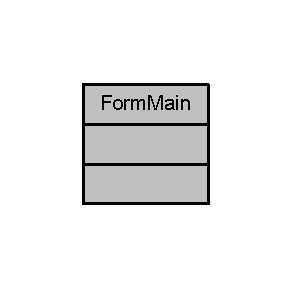
\includegraphics[width=140pt]{class_form_main__coll__graph}
\end{center}
\end{figure}


\subsection{Detailed Description}
Form\+Mainクラス 

The documentation for this class was generated from the following file\+:\begin{DoxyCompactItemize}
\item 
\hyperlink{_form_main_8cs}{Form\+Main.\+cs}\end{DoxyCompactItemize}

\hypertarget{class_reversi_form_1_1_hsl_color}{}\section{Reversi\+Form.\+Hsl\+Color Class Reference}
\label{class_reversi_form_1_1_hsl_color}\index{Reversi\+Form.\+Hsl\+Color@{Reversi\+Form.\+Hsl\+Color}}


H\+SL (H\+LS) カラーを表す  




Collaboration diagram for Reversi\+Form.\+Hsl\+Color\+:
\nopagebreak
\begin{figure}[H]
\begin{center}
\leavevmode
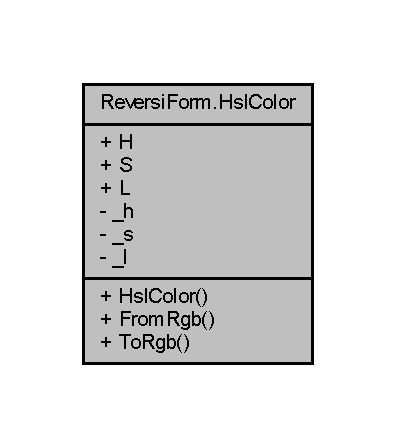
\includegraphics[width=190pt]{class_reversi_form_1_1_hsl_color__coll__graph}
\end{center}
\end{figure}
\subsection*{Public Member Functions}
\begin{DoxyCompactItemize}
\item 
\mbox{\Hypertarget{class_reversi_form_1_1_hsl_color_ada60003dff54b8b81df385bd37b23982}\label{class_reversi_form_1_1_hsl_color_ada60003dff54b8b81df385bd37b23982}} 
{\bfseries Hsl\+Color} (float hue, float saturation, float lightness)
\end{DoxyCompactItemize}
\subsection*{Static Public Member Functions}
\begin{DoxyCompactItemize}
\item 
static \hyperlink{class_reversi_form_1_1_hsl_color}{Hsl\+Color} \hyperlink{class_reversi_form_1_1_hsl_color_a1ef52b0701860ca2021e74e8ee369789}{From\+Rgb} (Color rgb)
\begin{DoxyCompactList}\small\item\em 指定した\+Colorから\+Hsl\+Colorを作成する \end{DoxyCompactList}\item 
static Color \hyperlink{class_reversi_form_1_1_hsl_color_aa7036039dd3abc7a1216be97656467df}{To\+Rgb} (\hyperlink{class_reversi_form_1_1_hsl_color}{Hsl\+Color} hsl)
\begin{DoxyCompactList}\small\item\em 指定した\+Hsl\+Colorから\+Colorを作成する \end{DoxyCompactList}\end{DoxyCompactItemize}
\subsection*{Properties}
\begin{DoxyCompactItemize}
\item 
float \hyperlink{class_reversi_form_1_1_hsl_color_ac1a2beeeae8bc7b8484ae7f3558fea53}{H}\hspace{0.3cm}{\ttfamily  \mbox{[}get\mbox{]}}
\begin{DoxyCompactList}\small\item\em 色相 (Hue) \end{DoxyCompactList}\item 
float \hyperlink{class_reversi_form_1_1_hsl_color_a0f9af27b3dee665ad51966d71e06c578}{S}\hspace{0.3cm}{\ttfamily  \mbox{[}get\mbox{]}}
\begin{DoxyCompactList}\small\item\em 彩度 (Saturation) \end{DoxyCompactList}\item 
float \hyperlink{class_reversi_form_1_1_hsl_color_a89e26c46eff241c066507625ddd5dc22}{L}\hspace{0.3cm}{\ttfamily  \mbox{[}get\mbox{]}}
\begin{DoxyCompactList}\small\item\em 輝度 (Lightness) \end{DoxyCompactList}\end{DoxyCompactItemize}
\subsection*{Private Attributes}
\begin{DoxyCompactItemize}
\item 
\mbox{\Hypertarget{class_reversi_form_1_1_hsl_color_a5a716a224d15c7fcf69651a92266149c}\label{class_reversi_form_1_1_hsl_color_a5a716a224d15c7fcf69651a92266149c}} 
float {\bfseries \+\_\+h}
\item 
\mbox{\Hypertarget{class_reversi_form_1_1_hsl_color_a2bf5f2795724a5a660db280c6c8828d8}\label{class_reversi_form_1_1_hsl_color_a2bf5f2795724a5a660db280c6c8828d8}} 
float {\bfseries \+\_\+s}
\item 
\mbox{\Hypertarget{class_reversi_form_1_1_hsl_color_af0394b4aa6c74f24eb86486b5c2bacc9}\label{class_reversi_form_1_1_hsl_color_af0394b4aa6c74f24eb86486b5c2bacc9}} 
float {\bfseries \+\_\+l}
\end{DoxyCompactItemize}


\subsection{Detailed Description}
H\+SL (H\+LS) カラーを表す 

Definition at line 28 of file Hsl\+Color.\+cs.



\subsection{Member Function Documentation}
\mbox{\Hypertarget{class_reversi_form_1_1_hsl_color_a1ef52b0701860ca2021e74e8ee369789}\label{class_reversi_form_1_1_hsl_color_a1ef52b0701860ca2021e74e8ee369789}} 
\index{Reversi\+Form\+::\+Hsl\+Color@{Reversi\+Form\+::\+Hsl\+Color}!From\+Rgb@{From\+Rgb}}
\index{From\+Rgb@{From\+Rgb}!Reversi\+Form\+::\+Hsl\+Color@{Reversi\+Form\+::\+Hsl\+Color}}
\subsubsection{\texorpdfstring{From\+Rgb()}{FromRgb()}}
{\footnotesize\ttfamily static \hyperlink{class_reversi_form_1_1_hsl_color}{Hsl\+Color} Reversi\+Form.\+Hsl\+Color.\+From\+Rgb (\begin{DoxyParamCaption}\item[{Color}]{rgb }\end{DoxyParamCaption})\hspace{0.3cm}{\ttfamily [static]}}



指定した\+Colorから\+Hsl\+Colorを作成する 


\begin{DoxyParams}{Parameters}
{\em rgb} & Color\\
\hline
\end{DoxyParams}
\begin{DoxyReturn}{Returns}
\hyperlink{class_reversi_form_1_1_hsl_color}{Hsl\+Color}
\end{DoxyReturn}


Definition at line 82 of file Hsl\+Color.\+cs.



Referenced by Reversi\+Form.\+Reversi.\+Draw\+Single\+Local().

Here is the caller graph for this function\+:
\nopagebreak
\begin{figure}[H]
\begin{center}
\leavevmode
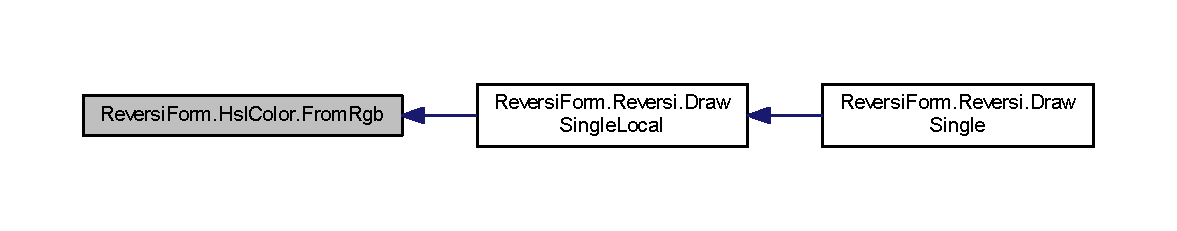
\includegraphics[width=350pt]{class_reversi_form_1_1_hsl_color_a1ef52b0701860ca2021e74e8ee369789_icgraph}
\end{center}
\end{figure}
\mbox{\Hypertarget{class_reversi_form_1_1_hsl_color_aa7036039dd3abc7a1216be97656467df}\label{class_reversi_form_1_1_hsl_color_aa7036039dd3abc7a1216be97656467df}} 
\index{Reversi\+Form\+::\+Hsl\+Color@{Reversi\+Form\+::\+Hsl\+Color}!To\+Rgb@{To\+Rgb}}
\index{To\+Rgb@{To\+Rgb}!Reversi\+Form\+::\+Hsl\+Color@{Reversi\+Form\+::\+Hsl\+Color}}
\subsubsection{\texorpdfstring{To\+Rgb()}{ToRgb()}}
{\footnotesize\ttfamily static Color Reversi\+Form.\+Hsl\+Color.\+To\+Rgb (\begin{DoxyParamCaption}\item[{\hyperlink{class_reversi_form_1_1_hsl_color}{Hsl\+Color}}]{hsl }\end{DoxyParamCaption})\hspace{0.3cm}{\ttfamily [static]}}



指定した\+Hsl\+Colorから\+Colorを作成する 


\begin{DoxyParams}{Parameters}
{\em hsl} & \hyperlink{class_reversi_form_1_1_hsl_color}{Hsl\+Color}\\
\hline
\end{DoxyParams}
\begin{DoxyReturn}{Returns}
Color
\end{DoxyReturn}


Definition at line 141 of file Hsl\+Color.\+cs.



Referenced by Reversi\+Form.\+Reversi.\+Draw\+Single\+Local().

Here is the caller graph for this function\+:
\nopagebreak
\begin{figure}[H]
\begin{center}
\leavevmode
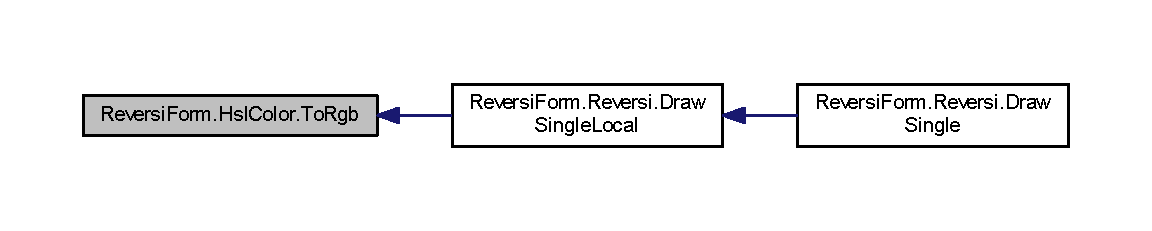
\includegraphics[width=350pt]{class_reversi_form_1_1_hsl_color_aa7036039dd3abc7a1216be97656467df_icgraph}
\end{center}
\end{figure}


\subsection{Property Documentation}
\mbox{\Hypertarget{class_reversi_form_1_1_hsl_color_ac1a2beeeae8bc7b8484ae7f3558fea53}\label{class_reversi_form_1_1_hsl_color_ac1a2beeeae8bc7b8484ae7f3558fea53}} 
\index{Reversi\+Form\+::\+Hsl\+Color@{Reversi\+Form\+::\+Hsl\+Color}!H@{H}}
\index{H@{H}!Reversi\+Form\+::\+Hsl\+Color@{Reversi\+Form\+::\+Hsl\+Color}}
\subsubsection{\texorpdfstring{H}{H}}
{\footnotesize\ttfamily float Reversi\+Form.\+Hsl\+Color.\+H\hspace{0.3cm}{\ttfamily [get]}}



色相 (Hue) 



Definition at line 35 of file Hsl\+Color.\+cs.



Referenced by Reversi\+Form.\+Reversi.\+Draw\+Single\+Local(), and Reversi\+Form.\+Hsl\+Color.\+To\+Rgb().

\mbox{\Hypertarget{class_reversi_form_1_1_hsl_color_a89e26c46eff241c066507625ddd5dc22}\label{class_reversi_form_1_1_hsl_color_a89e26c46eff241c066507625ddd5dc22}} 
\index{Reversi\+Form\+::\+Hsl\+Color@{Reversi\+Form\+::\+Hsl\+Color}!L@{L}}
\index{L@{L}!Reversi\+Form\+::\+Hsl\+Color@{Reversi\+Form\+::\+Hsl\+Color}}
\subsubsection{\texorpdfstring{L}{L}}
{\footnotesize\ttfamily float Reversi\+Form.\+Hsl\+Color.\+L\hspace{0.3cm}{\ttfamily [get]}}



輝度 (Lightness) 



Definition at line 53 of file Hsl\+Color.\+cs.



Referenced by Reversi\+Form.\+Reversi.\+Draw\+Single\+Local(), and Reversi\+Form.\+Hsl\+Color.\+To\+Rgb().

\mbox{\Hypertarget{class_reversi_form_1_1_hsl_color_a0f9af27b3dee665ad51966d71e06c578}\label{class_reversi_form_1_1_hsl_color_a0f9af27b3dee665ad51966d71e06c578}} 
\index{Reversi\+Form\+::\+Hsl\+Color@{Reversi\+Form\+::\+Hsl\+Color}!S@{S}}
\index{S@{S}!Reversi\+Form\+::\+Hsl\+Color@{Reversi\+Form\+::\+Hsl\+Color}}
\subsubsection{\texorpdfstring{S}{S}}
{\footnotesize\ttfamily float Reversi\+Form.\+Hsl\+Color.\+S\hspace{0.3cm}{\ttfamily [get]}}



彩度 (Saturation) 



Definition at line 44 of file Hsl\+Color.\+cs.



Referenced by Reversi\+Form.\+Reversi.\+Draw\+Single\+Local(), and Reversi\+Form.\+Hsl\+Color.\+To\+Rgb().



The documentation for this class was generated from the following file\+:\begin{DoxyCompactItemize}
\item 
Model/\hyperlink{_hsl_color_8cs}{Hsl\+Color.\+cs}\end{DoxyCompactItemize}

\hypertarget{class_reversi_form_1_1_my_reversi}{}\section{Reversi\+Form.\+My\+Reversi Class Reference}
\label{class_reversi_form_1_1_my_reversi}\index{Reversi\+Form.\+My\+Reversi@{Reversi\+Form.\+My\+Reversi}}


リバーシクラス  




Collaboration diagram for Reversi\+Form.\+My\+Reversi\+:
\nopagebreak
\begin{figure}[H]
\begin{center}
\leavevmode
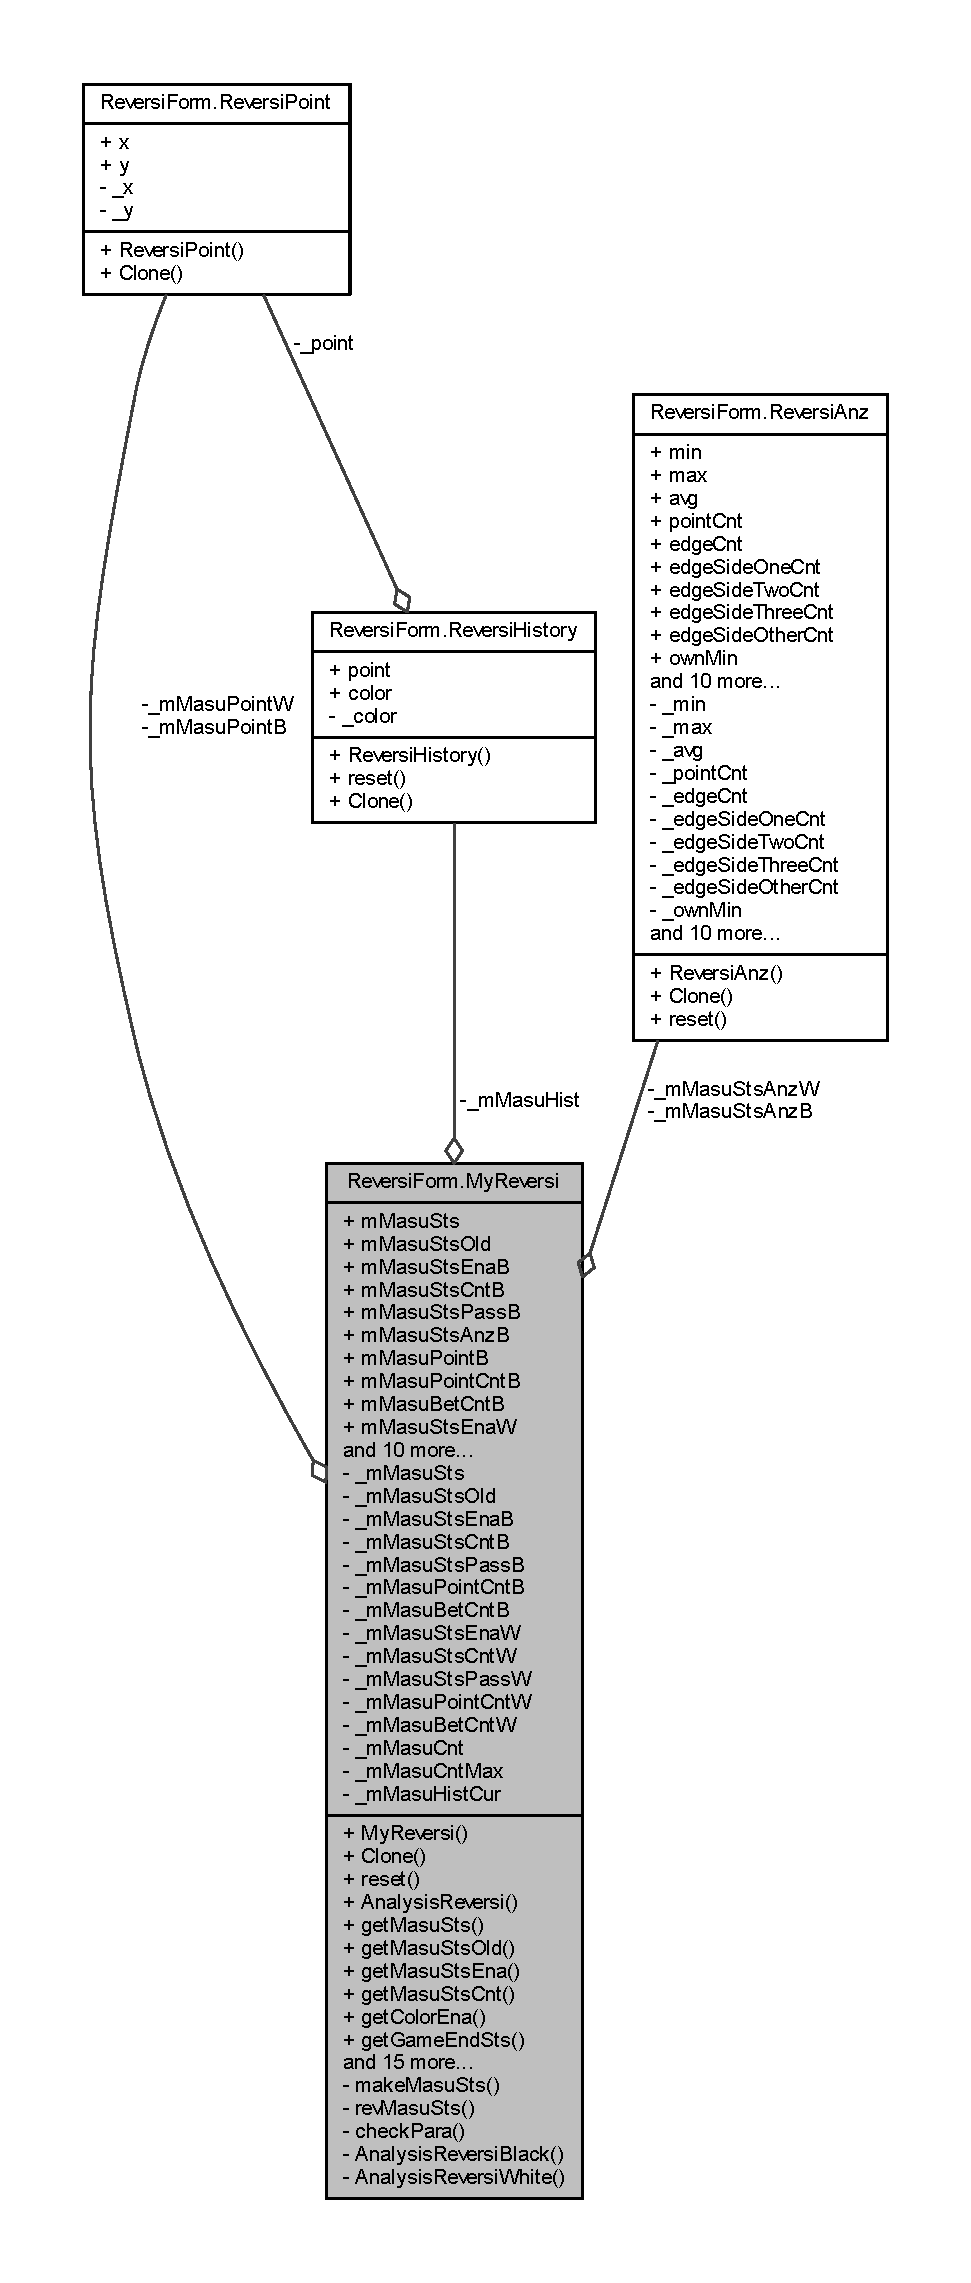
\includegraphics[height=550pt]{class_reversi_form_1_1_my_reversi__coll__graph}
\end{center}
\end{figure}
\subsection*{Public Member Functions}
\begin{DoxyCompactItemize}
\item 
\hyperlink{class_reversi_form_1_1_my_reversi_ab8c7a345a2e1d0978afd640d052f3827}{My\+Reversi} (int masu\+Cnt, int masu\+Max)
\begin{DoxyCompactList}\small\item\em コンストラクタ \end{DoxyCompactList}\item 
\hyperlink{class_reversi_form_1_1_my_reversi}{My\+Reversi} \hyperlink{class_reversi_form_1_1_my_reversi_aa340f79c0f7bb78750c410ce73ca7b99}{Clone} ()
\begin{DoxyCompactList}\small\item\em コピー \end{DoxyCompactList}\item 
void \hyperlink{class_reversi_form_1_1_my_reversi_aa8d8e839466c63462954080353cd4a9e}{reset} ()
\begin{DoxyCompactList}\small\item\em リセット \end{DoxyCompactList}\item 
void \hyperlink{class_reversi_form_1_1_my_reversi_afc9513cbba4f973c7d1ee92e0a0f3288}{Analysis\+Reversi} (int b\+Pass\+Ena, int w\+Pass\+Ena)
\begin{DoxyCompactList}\small\item\em 解析を行う \end{DoxyCompactList}\item 
int \hyperlink{class_reversi_form_1_1_my_reversi_ab6498c154199b58c418af1e0058736f6}{get\+Masu\+Sts} (int y, int x)
\begin{DoxyCompactList}\small\item\em マスステータスを取得 \end{DoxyCompactList}\item 
int \hyperlink{class_reversi_form_1_1_my_reversi_abd6f4b9d6355af3175ac885731338705}{get\+Masu\+Sts\+Old} (int y, int x)
\begin{DoxyCompactList}\small\item\em 以前のマスステータスを取得 \end{DoxyCompactList}\item 
int \hyperlink{class_reversi_form_1_1_my_reversi_ae8404068c47751d53c4b430d635a1bb2}{get\+Masu\+Sts\+Ena} (int color, int y, int x)
\begin{DoxyCompactList}\small\item\em 指定座標に指定色を置けるかチェック \end{DoxyCompactList}\item 
int \hyperlink{class_reversi_form_1_1_my_reversi_a26818336f7915237cf274e1fdff7ec4b}{get\+Masu\+Sts\+Cnt} (int color, int y, int x)
\begin{DoxyCompactList}\small\item\em 指定座標の獲得コマ数取得 \end{DoxyCompactList}\item 
int \hyperlink{class_reversi_form_1_1_my_reversi_a960e2691d2d106e5ad6036cfe9cf2503}{get\+Color\+Ena} (int color)
\begin{DoxyCompactList}\small\item\em 指定色が現在置ける場所があるかチェック \end{DoxyCompactList}\item 
int \hyperlink{class_reversi_form_1_1_my_reversi_aa39c8c111afeb4ea3bf2befbd9f1434b}{get\+Game\+End\+Sts} ()
\begin{DoxyCompactList}\small\item\em ゲーム終了かチェック \end{DoxyCompactList}\item 
int \hyperlink{class_reversi_form_1_1_my_reversi_a1f7ba86f6e8d5dd2fa472a8994e4e3c5}{set\+Masu\+Sts} (int color, int y, int x)
\begin{DoxyCompactList}\small\item\em 指定座標にコマを置く \end{DoxyCompactList}\item 
int \hyperlink{class_reversi_form_1_1_my_reversi_a940c5ec6841ffa050a53276815afcc9d}{set\+Masu\+Sts\+Forcibly} (int color, int y, int x)
\begin{DoxyCompactList}\small\item\em 指定座標にコマを強制的に置く \end{DoxyCompactList}\item 
int \hyperlink{class_reversi_form_1_1_my_reversi_af9573f1da0d89180a4dbbd98d41a05fb}{set\+Masu\+Cnt} (int cnt)
\begin{DoxyCompactList}\small\item\em マスの数変更 \end{DoxyCompactList}\item 
\hyperlink{class_reversi_form_1_1_reversi_point}{Reversi\+Point} \hyperlink{class_reversi_form_1_1_my_reversi_a58150a220368d7d7ae8ad01ee0120e71}{get\+Point} (int color, int num)
\begin{DoxyCompactList}\small\item\em ポイント座標取得 \end{DoxyCompactList}\item 
int \hyperlink{class_reversi_form_1_1_my_reversi_a7b5ebbdd9b7ff56d72185e6b89a50af8}{get\+Point\+Cnt} (int color)
\begin{DoxyCompactList}\small\item\em ポイント座標数取得 \end{DoxyCompactList}\item 
int \hyperlink{class_reversi_form_1_1_my_reversi_aa69640136727deb89addafae8e8e54cb}{get\+Bet\+Cnt} (int color)
\begin{DoxyCompactList}\small\item\em コマ数取得 \end{DoxyCompactList}\item 
int \hyperlink{class_reversi_form_1_1_my_reversi_a13c780ba2b5a346bd6fd295a0cc962f8}{get\+Pass\+Ena} (int color, int y, int x)
\begin{DoxyCompactList}\small\item\em パス判定 \end{DoxyCompactList}\item 
\hyperlink{class_reversi_form_1_1_reversi_history}{Reversi\+History} \hyperlink{class_reversi_form_1_1_my_reversi_a249dba624bda1144c23cc53f68c35c67}{get\+History} (int num)
\begin{DoxyCompactList}\small\item\em 履歴取得 \end{DoxyCompactList}\item 
int \hyperlink{class_reversi_form_1_1_my_reversi_a400dc82a921060bfdcf97a5fee721be1}{get\+History\+Cnt} ()
\begin{DoxyCompactList}\small\item\em 履歴数取得 \end{DoxyCompactList}\item 
\hyperlink{class_reversi_form_1_1_reversi_anz}{Reversi\+Anz} \hyperlink{class_reversi_form_1_1_my_reversi_af0170bf211a996c2285d0db926f2f0ae}{get\+Point\+Anz} (int color, int y, int x)
\begin{DoxyCompactList}\small\item\em ポイント座標解析取得 \end{DoxyCompactList}\item 
int \hyperlink{class_reversi_form_1_1_my_reversi_aa626cbf9735559841662c8fc413abb98}{check\+Edge} (int color, int y, int x)
\begin{DoxyCompactList}\small\item\em 角の隣に置いても角を取られないマス検索 \end{DoxyCompactList}\item 
int \hyperlink{class_reversi_form_1_1_my_reversi_a64216270f06c7c309d39bfcb681dd1b3}{get\+Edge\+Side\+Zero} (int y, int x)
\begin{DoxyCompactList}\small\item\em 指定座標が角か取得 \end{DoxyCompactList}\item 
int \hyperlink{class_reversi_form_1_1_my_reversi_a998eeefb18faecad172a6e1da4c70d7c}{get\+Edge\+Side\+One} (int y, int x)
\begin{DoxyCompactList}\small\item\em 指定座標が角の一つ手前か取得 \end{DoxyCompactList}\item 
int \hyperlink{class_reversi_form_1_1_my_reversi_a4b5395df3beb684f55b10bab91661c78}{get\+Edge\+Side\+Two} (int y, int x)
\begin{DoxyCompactList}\small\item\em 指定座標が角の二つ手前か取得 \end{DoxyCompactList}\item 
int \hyperlink{class_reversi_form_1_1_my_reversi_af6fee61bda5532c4c130e5660f7ce66f}{get\+Edge\+Side\+Three} (int y, int x)
\begin{DoxyCompactList}\small\item\em 指定座標が角の三つ以上手前か取得 \end{DoxyCompactList}\end{DoxyCompactItemize}
\subsection*{Properties}
\begin{DoxyCompactItemize}
\item 
\mbox{\Hypertarget{class_reversi_form_1_1_my_reversi_a03f90fbb31784b8d2bbff05d6b30ec1f}\label{class_reversi_form_1_1_my_reversi_a03f90fbb31784b8d2bbff05d6b30ec1f}} 
int \mbox{[},\mbox{]} {\bfseries m\+Masu\+Sts}\hspace{0.3cm}{\ttfamily  \mbox{[}get, set\mbox{]}}
\item 
\mbox{\Hypertarget{class_reversi_form_1_1_my_reversi_ab315833c016b108b23b8f49bbbf9311c}\label{class_reversi_form_1_1_my_reversi_ab315833c016b108b23b8f49bbbf9311c}} 
int \mbox{[},\mbox{]} {\bfseries m\+Masu\+Sts\+Old}\hspace{0.3cm}{\ttfamily  \mbox{[}get, set\mbox{]}}
\item 
\mbox{\Hypertarget{class_reversi_form_1_1_my_reversi_adae7be9110010b23dfd76833c55dc43e}\label{class_reversi_form_1_1_my_reversi_adae7be9110010b23dfd76833c55dc43e}} 
int \mbox{[},\mbox{]} {\bfseries m\+Masu\+Sts\+EnaB}\hspace{0.3cm}{\ttfamily  \mbox{[}get, set\mbox{]}}
\item 
\mbox{\Hypertarget{class_reversi_form_1_1_my_reversi_aeff6f2bc99d1cee48d46ead3a7dd6728}\label{class_reversi_form_1_1_my_reversi_aeff6f2bc99d1cee48d46ead3a7dd6728}} 
int \mbox{[},\mbox{]} {\bfseries m\+Masu\+Sts\+CntB}\hspace{0.3cm}{\ttfamily  \mbox{[}get, set\mbox{]}}
\item 
\mbox{\Hypertarget{class_reversi_form_1_1_my_reversi_a25a2d605244dd6db2e14944ec1250880}\label{class_reversi_form_1_1_my_reversi_a25a2d605244dd6db2e14944ec1250880}} 
int \mbox{[},\mbox{]} {\bfseries m\+Masu\+Sts\+PassB}\hspace{0.3cm}{\ttfamily  \mbox{[}get, set\mbox{]}}
\item 
\mbox{\Hypertarget{class_reversi_form_1_1_my_reversi_a2cb36dfb933c2a3450f4a7a22205c4c3}\label{class_reversi_form_1_1_my_reversi_a2cb36dfb933c2a3450f4a7a22205c4c3}} 
\hyperlink{class_reversi_form_1_1_reversi_anz}{Reversi\+Anz} \mbox{[},\mbox{]} {\bfseries m\+Masu\+Sts\+AnzB}\hspace{0.3cm}{\ttfamily  \mbox{[}get, set\mbox{]}}
\item 
\mbox{\Hypertarget{class_reversi_form_1_1_my_reversi_a343e9f4d9c5dc09c1ed28bcec45f03a6}\label{class_reversi_form_1_1_my_reversi_a343e9f4d9c5dc09c1ed28bcec45f03a6}} 
\hyperlink{class_reversi_form_1_1_reversi_point}{Reversi\+Point} \mbox{[}$\,$\mbox{]} {\bfseries m\+Masu\+PointB}\hspace{0.3cm}{\ttfamily  \mbox{[}get, set\mbox{]}}
\item 
\mbox{\Hypertarget{class_reversi_form_1_1_my_reversi_a71f276a0873e4d7b8dba6861fd079c95}\label{class_reversi_form_1_1_my_reversi_a71f276a0873e4d7b8dba6861fd079c95}} 
int {\bfseries m\+Masu\+Point\+CntB}\hspace{0.3cm}{\ttfamily  \mbox{[}get, set\mbox{]}}
\item 
\mbox{\Hypertarget{class_reversi_form_1_1_my_reversi_ae875f86393f2307557bd38bb5feb6cda}\label{class_reversi_form_1_1_my_reversi_ae875f86393f2307557bd38bb5feb6cda}} 
int {\bfseries m\+Masu\+Bet\+CntB}\hspace{0.3cm}{\ttfamily  \mbox{[}get, set\mbox{]}}
\item 
\mbox{\Hypertarget{class_reversi_form_1_1_my_reversi_af87a624d11b7f42a8116731ddf8b6b46}\label{class_reversi_form_1_1_my_reversi_af87a624d11b7f42a8116731ddf8b6b46}} 
int \mbox{[},\mbox{]} {\bfseries m\+Masu\+Sts\+EnaW}\hspace{0.3cm}{\ttfamily  \mbox{[}get, set\mbox{]}}
\item 
\mbox{\Hypertarget{class_reversi_form_1_1_my_reversi_a9485a7739382438b80a851d44556ee40}\label{class_reversi_form_1_1_my_reversi_a9485a7739382438b80a851d44556ee40}} 
int \mbox{[},\mbox{]} {\bfseries m\+Masu\+Sts\+CntW}\hspace{0.3cm}{\ttfamily  \mbox{[}get, set\mbox{]}}
\item 
\mbox{\Hypertarget{class_reversi_form_1_1_my_reversi_aa43e8dee73aeec95d8a43bde0dc83dab}\label{class_reversi_form_1_1_my_reversi_aa43e8dee73aeec95d8a43bde0dc83dab}} 
int \mbox{[},\mbox{]} {\bfseries m\+Masu\+Sts\+PassW}\hspace{0.3cm}{\ttfamily  \mbox{[}get, set\mbox{]}}
\item 
\mbox{\Hypertarget{class_reversi_form_1_1_my_reversi_a39700a9ea73f0c8bc79be318784691c5}\label{class_reversi_form_1_1_my_reversi_a39700a9ea73f0c8bc79be318784691c5}} 
\hyperlink{class_reversi_form_1_1_reversi_anz}{Reversi\+Anz} \mbox{[},\mbox{]} {\bfseries m\+Masu\+Sts\+AnzW}\hspace{0.3cm}{\ttfamily  \mbox{[}get, set\mbox{]}}
\item 
\mbox{\Hypertarget{class_reversi_form_1_1_my_reversi_aef734c975cbffcca566b5169f72fd816}\label{class_reversi_form_1_1_my_reversi_aef734c975cbffcca566b5169f72fd816}} 
\hyperlink{class_reversi_form_1_1_reversi_point}{Reversi\+Point} \mbox{[}$\,$\mbox{]} {\bfseries m\+Masu\+PointW}\hspace{0.3cm}{\ttfamily  \mbox{[}get, set\mbox{]}}
\item 
\mbox{\Hypertarget{class_reversi_form_1_1_my_reversi_a2bd4f43a7e575a48aea9c8fb23ecbb56}\label{class_reversi_form_1_1_my_reversi_a2bd4f43a7e575a48aea9c8fb23ecbb56}} 
int {\bfseries m\+Masu\+Point\+CntW}\hspace{0.3cm}{\ttfamily  \mbox{[}get, set\mbox{]}}
\item 
\mbox{\Hypertarget{class_reversi_form_1_1_my_reversi_a87cbfee2c58f5147ed820087301334dc}\label{class_reversi_form_1_1_my_reversi_a87cbfee2c58f5147ed820087301334dc}} 
int {\bfseries m\+Masu\+Bet\+CntW}\hspace{0.3cm}{\ttfamily  \mbox{[}get, set\mbox{]}}
\item 
\mbox{\Hypertarget{class_reversi_form_1_1_my_reversi_aa22d12821c2bae0187afff080e4cbe38}\label{class_reversi_form_1_1_my_reversi_aa22d12821c2bae0187afff080e4cbe38}} 
int {\bfseries m\+Masu\+Cnt}\hspace{0.3cm}{\ttfamily  \mbox{[}get, set\mbox{]}}
\item 
\mbox{\Hypertarget{class_reversi_form_1_1_my_reversi_a06a8fdc5f67534e63caaec70009bfee7}\label{class_reversi_form_1_1_my_reversi_a06a8fdc5f67534e63caaec70009bfee7}} 
int {\bfseries m\+Masu\+Cnt\+Max}\hspace{0.3cm}{\ttfamily  \mbox{[}get, set\mbox{]}}
\item 
\mbox{\Hypertarget{class_reversi_form_1_1_my_reversi_a2d28fda045dd88cc244b2f0d3b695a56}\label{class_reversi_form_1_1_my_reversi_a2d28fda045dd88cc244b2f0d3b695a56}} 
int {\bfseries m\+Masu\+Hist\+Cur}\hspace{0.3cm}{\ttfamily  \mbox{[}get, set\mbox{]}}
\item 
\mbox{\Hypertarget{class_reversi_form_1_1_my_reversi_aff002005445d19802d7f0fa41abedb4b}\label{class_reversi_form_1_1_my_reversi_aff002005445d19802d7f0fa41abedb4b}} 
\hyperlink{class_reversi_form_1_1_reversi_history}{Reversi\+History} \mbox{[}$\,$\mbox{]} {\bfseries m\+Masu\+Hist}\hspace{0.3cm}{\ttfamily  \mbox{[}get, set\mbox{]}}
\end{DoxyCompactItemize}
\subsection*{Private Member Functions}
\begin{DoxyCompactItemize}
\item 
int \hyperlink{class_reversi_form_1_1_my_reversi_a379ac04ab0e8e9fc819ef3ceeba63e58}{make\+Masu\+Sts} (int color)
\begin{DoxyCompactList}\small\item\em 各コマの置ける場所等のステータス作成 \end{DoxyCompactList}\item 
void \hyperlink{class_reversi_form_1_1_my_reversi_a990acf71124e50643c0774c38f8f634b}{rev\+Masu\+Sts} (int color, int y, int x)
\begin{DoxyCompactList}\small\item\em コマをひっくり返す \end{DoxyCompactList}\item 
int \hyperlink{class_reversi_form_1_1_my_reversi_a7d861112d0ddeb404cd3e8d8f5c2756b}{check\+Para} (int para, int min, int max)
\begin{DoxyCompactList}\small\item\em パラメーター範囲チェック \end{DoxyCompactList}\item 
void \hyperlink{class_reversi_form_1_1_my_reversi_adfa9fda128ee816da9b32009326c5a15}{Analysis\+Reversi\+Black} ()
\begin{DoxyCompactList}\small\item\em 解析を行う(黒) \end{DoxyCompactList}\item 
void \hyperlink{class_reversi_form_1_1_my_reversi_a2fac17b7121d91063e2d759487f1ed18}{Analysis\+Reversi\+White} ()
\begin{DoxyCompactList}\small\item\em 解析を行う(白) \end{DoxyCompactList}\end{DoxyCompactItemize}
\subsection*{Private Attributes}
\begin{DoxyCompactItemize}
\item 
\mbox{\Hypertarget{class_reversi_form_1_1_my_reversi_aef0be9a7d414448f400a6350a1118acf}\label{class_reversi_form_1_1_my_reversi_aef0be9a7d414448f400a6350a1118acf}} 
int \mbox{[},\mbox{]} \hyperlink{class_reversi_form_1_1_my_reversi_aef0be9a7d414448f400a6350a1118acf}{\+\_\+m\+Masu\+Sts}
\begin{DoxyCompactList}\small\item\em マスの状態 \end{DoxyCompactList}\item 
\mbox{\Hypertarget{class_reversi_form_1_1_my_reversi_a722513f8f511854fe56b292135549958}\label{class_reversi_form_1_1_my_reversi_a722513f8f511854fe56b292135549958}} 
int \mbox{[},\mbox{]} \hyperlink{class_reversi_form_1_1_my_reversi_a722513f8f511854fe56b292135549958}{\+\_\+m\+Masu\+Sts\+Old}
\begin{DoxyCompactList}\small\item\em 以前のマスの状態 \end{DoxyCompactList}\item 
\mbox{\Hypertarget{class_reversi_form_1_1_my_reversi_a4a031cd96cc7ecb89a92dd335e62143c}\label{class_reversi_form_1_1_my_reversi_a4a031cd96cc7ecb89a92dd335e62143c}} 
int \mbox{[},\mbox{]} \hyperlink{class_reversi_form_1_1_my_reversi_a4a031cd96cc7ecb89a92dd335e62143c}{\+\_\+m\+Masu\+Sts\+EnaB}
\begin{DoxyCompactList}\small\item\em 黒の置ける場所 \end{DoxyCompactList}\item 
\mbox{\Hypertarget{class_reversi_form_1_1_my_reversi_ae5c9bcdfb08f78d463b75dcd0fa29faf}\label{class_reversi_form_1_1_my_reversi_ae5c9bcdfb08f78d463b75dcd0fa29faf}} 
int \mbox{[},\mbox{]} \hyperlink{class_reversi_form_1_1_my_reversi_ae5c9bcdfb08f78d463b75dcd0fa29faf}{\+\_\+m\+Masu\+Sts\+CntB}
\begin{DoxyCompactList}\small\item\em 黒の獲得コマ数 \end{DoxyCompactList}\item 
\mbox{\Hypertarget{class_reversi_form_1_1_my_reversi_a239d0b04ee92c19fe0f60dd2f4e45d76}\label{class_reversi_form_1_1_my_reversi_a239d0b04ee92c19fe0f60dd2f4e45d76}} 
int \mbox{[},\mbox{]} \hyperlink{class_reversi_form_1_1_my_reversi_a239d0b04ee92c19fe0f60dd2f4e45d76}{\+\_\+m\+Masu\+Sts\+PassB}
\begin{DoxyCompactList}\small\item\em 黒が相手をパスさせる場所 \end{DoxyCompactList}\item 
\mbox{\Hypertarget{class_reversi_form_1_1_my_reversi_afeb60d6d64829a2c0001c46aafc20492}\label{class_reversi_form_1_1_my_reversi_afeb60d6d64829a2c0001c46aafc20492}} 
\hyperlink{class_reversi_form_1_1_reversi_anz}{Reversi\+Anz} \mbox{[},\mbox{]} \hyperlink{class_reversi_form_1_1_my_reversi_afeb60d6d64829a2c0001c46aafc20492}{\+\_\+m\+Masu\+Sts\+AnzB}
\begin{DoxyCompactList}\small\item\em 黒がその場所に置いた場合の解析結果 \end{DoxyCompactList}\item 
\mbox{\Hypertarget{class_reversi_form_1_1_my_reversi_a52c2068d950d2a9564f2c7954aa23955}\label{class_reversi_form_1_1_my_reversi_a52c2068d950d2a9564f2c7954aa23955}} 
\hyperlink{class_reversi_form_1_1_reversi_point}{Reversi\+Point} \mbox{[}$\,$\mbox{]} \hyperlink{class_reversi_form_1_1_my_reversi_a52c2068d950d2a9564f2c7954aa23955}{\+\_\+m\+Masu\+PointB}
\begin{DoxyCompactList}\small\item\em 黒の置ける場所座標一覧 \end{DoxyCompactList}\item 
\mbox{\Hypertarget{class_reversi_form_1_1_my_reversi_adec5d94bb73a7de5c687cce708cc6235}\label{class_reversi_form_1_1_my_reversi_adec5d94bb73a7de5c687cce708cc6235}} 
int \hyperlink{class_reversi_form_1_1_my_reversi_adec5d94bb73a7de5c687cce708cc6235}{\+\_\+m\+Masu\+Point\+CntB}
\begin{DoxyCompactList}\small\item\em 黒の置ける場所座標一覧数 \end{DoxyCompactList}\item 
\mbox{\Hypertarget{class_reversi_form_1_1_my_reversi_ad860e5a347f3a9d4ba029dc58b943357}\label{class_reversi_form_1_1_my_reversi_ad860e5a347f3a9d4ba029dc58b943357}} 
int \hyperlink{class_reversi_form_1_1_my_reversi_ad860e5a347f3a9d4ba029dc58b943357}{\+\_\+m\+Masu\+Bet\+CntB}
\begin{DoxyCompactList}\small\item\em 黒コマ数 \end{DoxyCompactList}\item 
\mbox{\Hypertarget{class_reversi_form_1_1_my_reversi_aa57338421f9bd268eea1b2ba4994c728}\label{class_reversi_form_1_1_my_reversi_aa57338421f9bd268eea1b2ba4994c728}} 
int \mbox{[},\mbox{]} \hyperlink{class_reversi_form_1_1_my_reversi_aa57338421f9bd268eea1b2ba4994c728}{\+\_\+m\+Masu\+Sts\+EnaW}
\begin{DoxyCompactList}\small\item\em 白の置ける場所 \end{DoxyCompactList}\item 
\mbox{\Hypertarget{class_reversi_form_1_1_my_reversi_a0df3fdfd0606eea5df0e9db119b0a740}\label{class_reversi_form_1_1_my_reversi_a0df3fdfd0606eea5df0e9db119b0a740}} 
int \mbox{[},\mbox{]} \hyperlink{class_reversi_form_1_1_my_reversi_a0df3fdfd0606eea5df0e9db119b0a740}{\+\_\+m\+Masu\+Sts\+CntW}
\begin{DoxyCompactList}\small\item\em 白の獲得コマ数 \end{DoxyCompactList}\item 
\mbox{\Hypertarget{class_reversi_form_1_1_my_reversi_af6c99c0854fed80f2f3f80d851563699}\label{class_reversi_form_1_1_my_reversi_af6c99c0854fed80f2f3f80d851563699}} 
int \mbox{[},\mbox{]} \hyperlink{class_reversi_form_1_1_my_reversi_af6c99c0854fed80f2f3f80d851563699}{\+\_\+m\+Masu\+Sts\+PassW}
\begin{DoxyCompactList}\small\item\em 白が相手をパスさせる場所 \end{DoxyCompactList}\item 
\mbox{\Hypertarget{class_reversi_form_1_1_my_reversi_a7d9e85bcb2c5fdd79d5e6418dc8344ac}\label{class_reversi_form_1_1_my_reversi_a7d9e85bcb2c5fdd79d5e6418dc8344ac}} 
\hyperlink{class_reversi_form_1_1_reversi_anz}{Reversi\+Anz} \mbox{[},\mbox{]} \hyperlink{class_reversi_form_1_1_my_reversi_a7d9e85bcb2c5fdd79d5e6418dc8344ac}{\+\_\+m\+Masu\+Sts\+AnzW}
\begin{DoxyCompactList}\small\item\em 白がその場所に置いた場合の解析結果 \end{DoxyCompactList}\item 
\mbox{\Hypertarget{class_reversi_form_1_1_my_reversi_a5dc23afff81506036e3ed0240de30f00}\label{class_reversi_form_1_1_my_reversi_a5dc23afff81506036e3ed0240de30f00}} 
\hyperlink{class_reversi_form_1_1_reversi_point}{Reversi\+Point} \mbox{[}$\,$\mbox{]} \hyperlink{class_reversi_form_1_1_my_reversi_a5dc23afff81506036e3ed0240de30f00}{\+\_\+m\+Masu\+PointW}
\begin{DoxyCompactList}\small\item\em 白の置ける場所座標一覧 \end{DoxyCompactList}\item 
\mbox{\Hypertarget{class_reversi_form_1_1_my_reversi_a082b5c3bcac1a3bb2ec8902753466e78}\label{class_reversi_form_1_1_my_reversi_a082b5c3bcac1a3bb2ec8902753466e78}} 
int \hyperlink{class_reversi_form_1_1_my_reversi_a082b5c3bcac1a3bb2ec8902753466e78}{\+\_\+m\+Masu\+Point\+CntW}
\begin{DoxyCompactList}\small\item\em 白の置ける場所座標一覧数 \end{DoxyCompactList}\item 
\mbox{\Hypertarget{class_reversi_form_1_1_my_reversi_a99a2f985b8f54a1f4d21f33aeb909c51}\label{class_reversi_form_1_1_my_reversi_a99a2f985b8f54a1f4d21f33aeb909c51}} 
int \hyperlink{class_reversi_form_1_1_my_reversi_a99a2f985b8f54a1f4d21f33aeb909c51}{\+\_\+m\+Masu\+Bet\+CntW}
\begin{DoxyCompactList}\small\item\em 白コマ数 \end{DoxyCompactList}\item 
\mbox{\Hypertarget{class_reversi_form_1_1_my_reversi_ae2c52ad6b09c617a255e589663e87723}\label{class_reversi_form_1_1_my_reversi_ae2c52ad6b09c617a255e589663e87723}} 
int \hyperlink{class_reversi_form_1_1_my_reversi_ae2c52ad6b09c617a255e589663e87723}{\+\_\+m\+Masu\+Cnt}
\begin{DoxyCompactList}\small\item\em 縦横マス数 \end{DoxyCompactList}\item 
\mbox{\Hypertarget{class_reversi_form_1_1_my_reversi_a4c890a1c4bfaff4e9b3855096efd002d}\label{class_reversi_form_1_1_my_reversi_a4c890a1c4bfaff4e9b3855096efd002d}} 
int \hyperlink{class_reversi_form_1_1_my_reversi_a4c890a1c4bfaff4e9b3855096efd002d}{\+\_\+m\+Masu\+Cnt\+Max}
\begin{DoxyCompactList}\small\item\em 縦横マス最大数 \end{DoxyCompactList}\item 
\mbox{\Hypertarget{class_reversi_form_1_1_my_reversi_a841c9b849777916f377232bca25e2808}\label{class_reversi_form_1_1_my_reversi_a841c9b849777916f377232bca25e2808}} 
int \hyperlink{class_reversi_form_1_1_my_reversi_a841c9b849777916f377232bca25e2808}{\+\_\+m\+Masu\+Hist\+Cur}
\begin{DoxyCompactList}\small\item\em 履歴現在位置 \end{DoxyCompactList}\item 
\mbox{\Hypertarget{class_reversi_form_1_1_my_reversi_af1c98962d82f9747088953345d434e7f}\label{class_reversi_form_1_1_my_reversi_af1c98962d82f9747088953345d434e7f}} 
\hyperlink{class_reversi_form_1_1_reversi_history}{Reversi\+History} \mbox{[}$\,$\mbox{]} \hyperlink{class_reversi_form_1_1_my_reversi_af1c98962d82f9747088953345d434e7f}{\+\_\+m\+Masu\+Hist}
\begin{DoxyCompactList}\small\item\em 履歴 \end{DoxyCompactList}\end{DoxyCompactItemize}


\subsection{Detailed Description}
リバーシクラス 

Definition at line 30 of file My\+Reversi.\+cs.



\subsection{Constructor \& Destructor Documentation}
\mbox{\Hypertarget{class_reversi_form_1_1_my_reversi_ab8c7a345a2e1d0978afd640d052f3827}\label{class_reversi_form_1_1_my_reversi_ab8c7a345a2e1d0978afd640d052f3827}} 
\index{Reversi\+Form\+::\+My\+Reversi@{Reversi\+Form\+::\+My\+Reversi}!My\+Reversi@{My\+Reversi}}
\index{My\+Reversi@{My\+Reversi}!Reversi\+Form\+::\+My\+Reversi@{Reversi\+Form\+::\+My\+Reversi}}
\subsubsection{\texorpdfstring{My\+Reversi()}{MyReversi()}}
{\footnotesize\ttfamily Reversi\+Form.\+My\+Reversi.\+My\+Reversi (\begin{DoxyParamCaption}\item[{int}]{masu\+Cnt,  }\item[{int}]{masu\+Max }\end{DoxyParamCaption})}



コンストラクタ 


\begin{DoxyParams}[1]{Parameters}
\mbox{\tt in}  & {\em int} & masu\+Cnt 縦横マス数 \\
\hline
\mbox{\tt in}  & {\em int} & masu\+Max 縦横マス最大数 \\
\hline
\end{DoxyParams}
\begin{DoxyReturn}{Returns}
ありません 
\end{DoxyReturn}
\begin{DoxyAuthor}{Author}
Yuta Yoshinaga 
\end{DoxyAuthor}
\begin{DoxyDate}{Date}
2017.\+10.\+20 
\end{DoxyDate}


Definition at line 168 of file My\+Reversi.\+cs.

Here is the call graph for this function\+:
\nopagebreak
\begin{figure}[H]
\begin{center}
\leavevmode
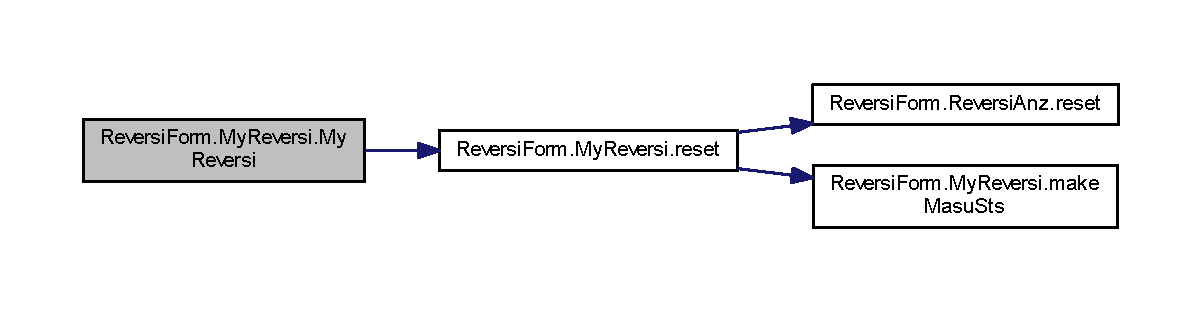
\includegraphics[width=350pt]{class_reversi_form_1_1_my_reversi_ab8c7a345a2e1d0978afd640d052f3827_cgraph}
\end{center}
\end{figure}


\subsection{Member Function Documentation}
\mbox{\Hypertarget{class_reversi_form_1_1_my_reversi_afc9513cbba4f973c7d1ee92e0a0f3288}\label{class_reversi_form_1_1_my_reversi_afc9513cbba4f973c7d1ee92e0a0f3288}} 
\index{Reversi\+Form\+::\+My\+Reversi@{Reversi\+Form\+::\+My\+Reversi}!Analysis\+Reversi@{Analysis\+Reversi}}
\index{Analysis\+Reversi@{Analysis\+Reversi}!Reversi\+Form\+::\+My\+Reversi@{Reversi\+Form\+::\+My\+Reversi}}
\subsubsection{\texorpdfstring{Analysis\+Reversi()}{AnalysisReversi()}}
{\footnotesize\ttfamily void Reversi\+Form.\+My\+Reversi.\+Analysis\+Reversi (\begin{DoxyParamCaption}\item[{int}]{b\+Pass\+Ena,  }\item[{int}]{w\+Pass\+Ena }\end{DoxyParamCaption})}



解析を行う 


\begin{DoxyParams}[1]{Parameters}
\mbox{\tt in}  & {\em int} & b\+Pass\+Ena 1=黒パス有効 \\
\hline
\mbox{\tt in}  & {\em int} & w\+Pass\+Ena 1=白パス有効 \\
\hline
\end{DoxyParams}
\begin{DoxyReturn}{Returns}
ありません 
\end{DoxyReturn}
\begin{DoxyAuthor}{Author}
Yuta Yoshinaga 
\end{DoxyAuthor}
\begin{DoxyDate}{Date}
2017.\+10.\+20 
\end{DoxyDate}


Definition at line 948 of file My\+Reversi.\+cs.



Referenced by Reversi\+Form.\+Reversi\+Play.\+reset(), Reversi\+Form.\+Reversi\+Play.\+reversi\+Play(), and Reversi\+Form.\+Reversi\+Play.\+reversi\+Play\+Cpu().

Here is the call graph for this function\+:
\nopagebreak
\begin{figure}[H]
\begin{center}
\leavevmode
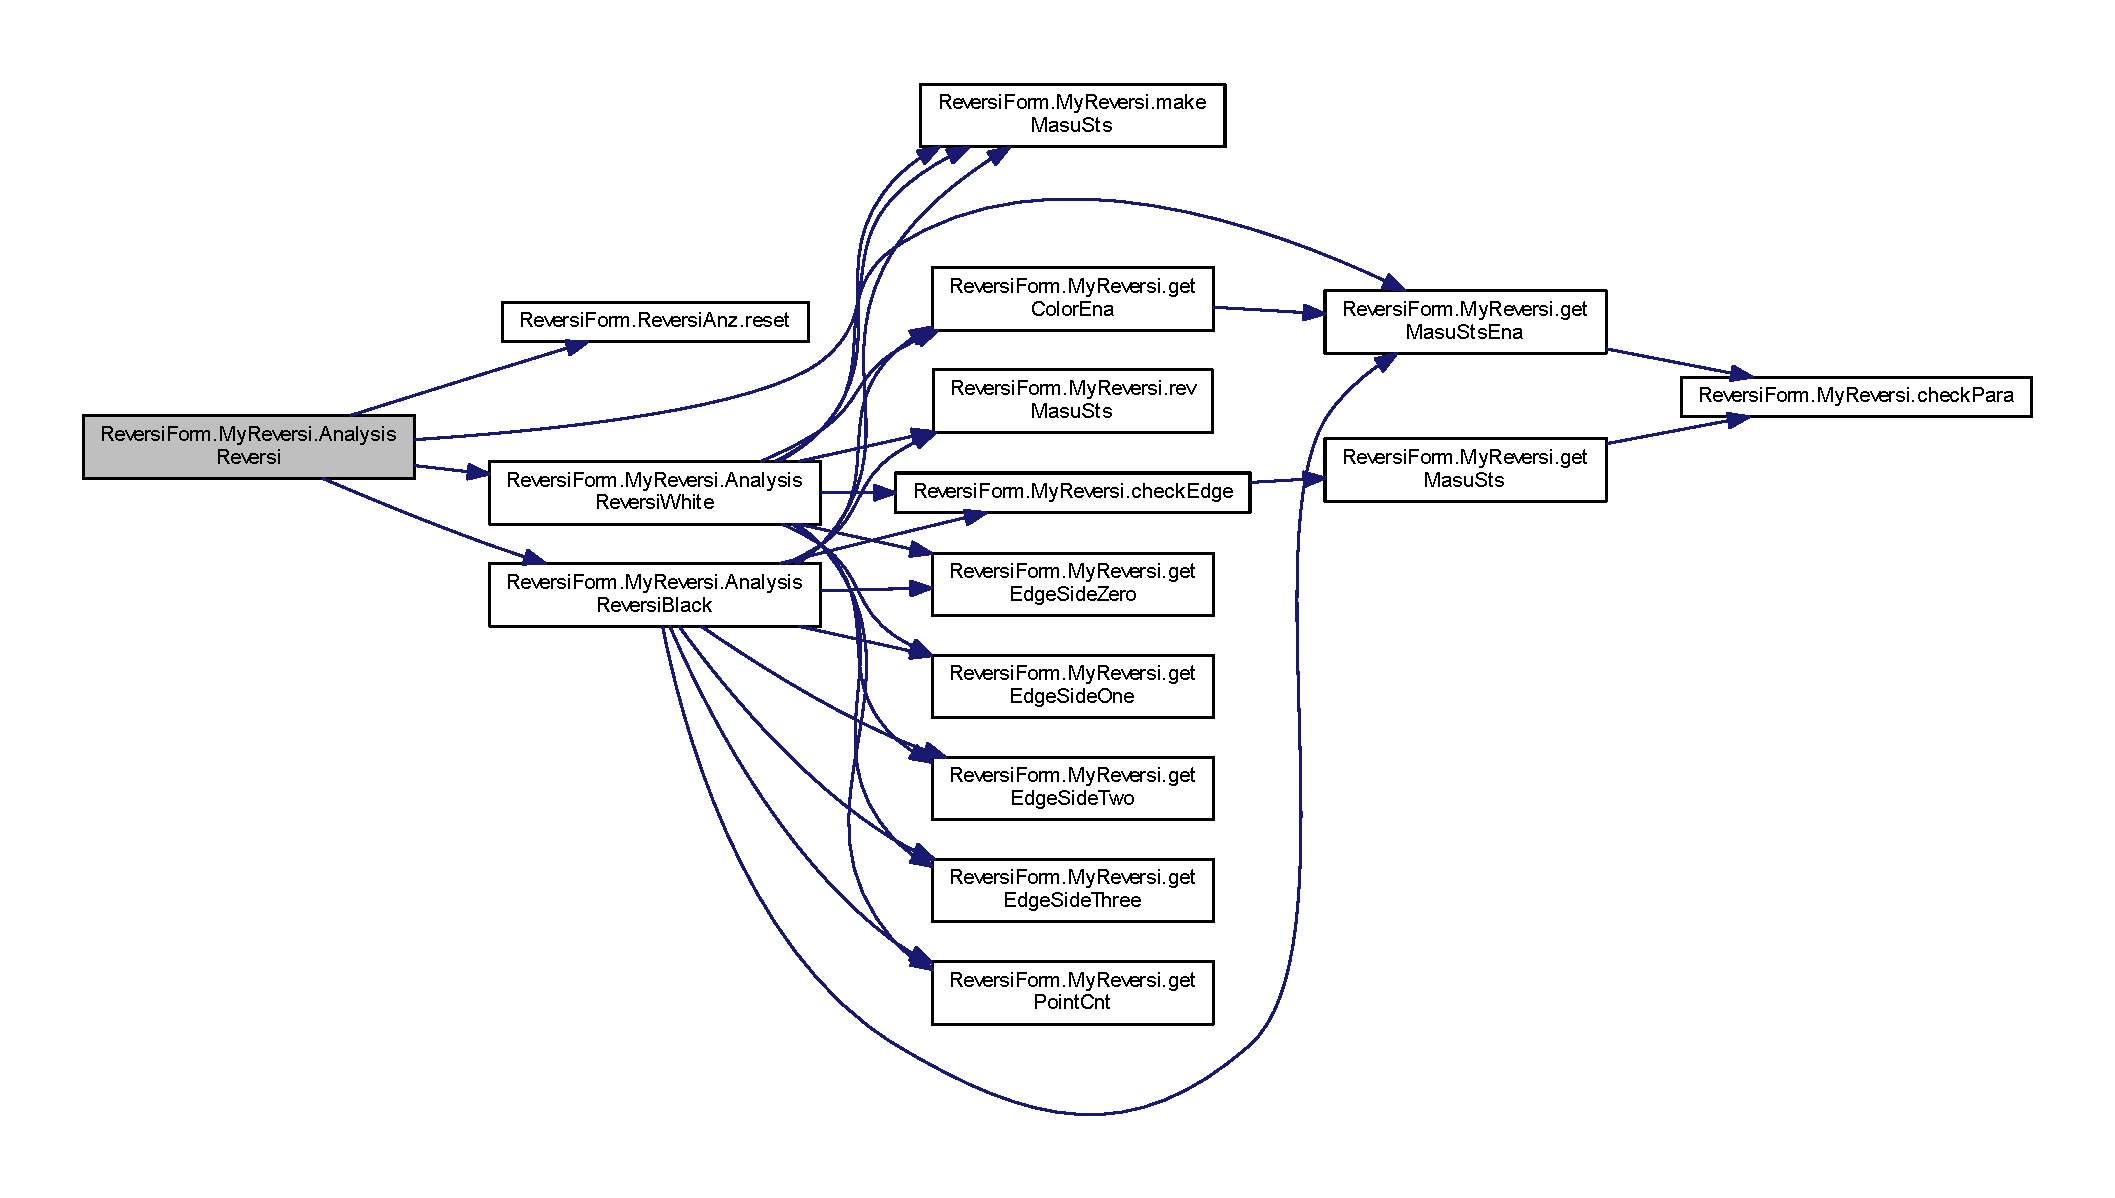
\includegraphics[width=350pt]{class_reversi_form_1_1_my_reversi_afc9513cbba4f973c7d1ee92e0a0f3288_cgraph}
\end{center}
\end{figure}
Here is the caller graph for this function\+:
\nopagebreak
\begin{figure}[H]
\begin{center}
\leavevmode
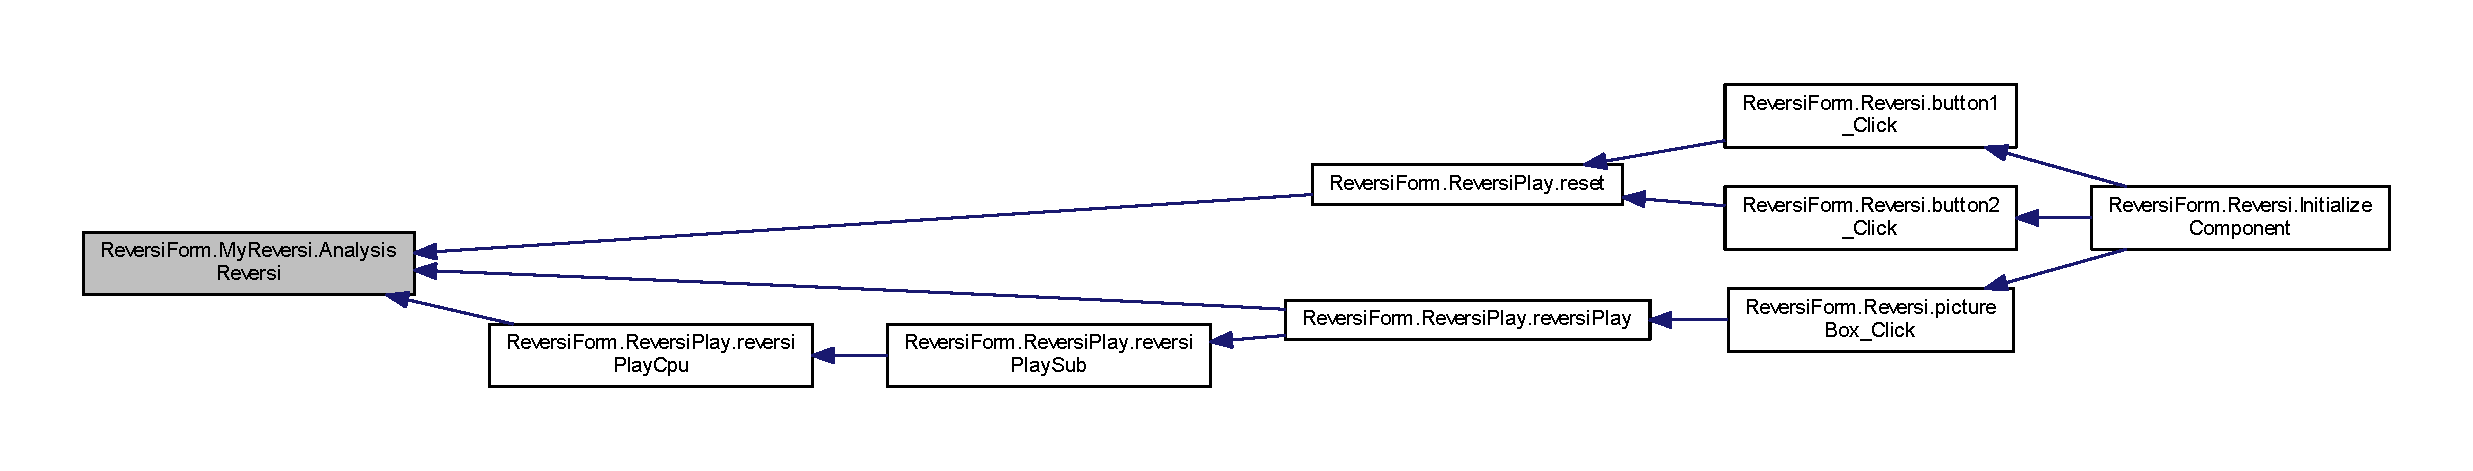
\includegraphics[width=350pt]{class_reversi_form_1_1_my_reversi_afc9513cbba4f973c7d1ee92e0a0f3288_icgraph}
\end{center}
\end{figure}
\mbox{\Hypertarget{class_reversi_form_1_1_my_reversi_adfa9fda128ee816da9b32009326c5a15}\label{class_reversi_form_1_1_my_reversi_adfa9fda128ee816da9b32009326c5a15}} 
\index{Reversi\+Form\+::\+My\+Reversi@{Reversi\+Form\+::\+My\+Reversi}!Analysis\+Reversi\+Black@{Analysis\+Reversi\+Black}}
\index{Analysis\+Reversi\+Black@{Analysis\+Reversi\+Black}!Reversi\+Form\+::\+My\+Reversi@{Reversi\+Form\+::\+My\+Reversi}}
\subsubsection{\texorpdfstring{Analysis\+Reversi\+Black()}{AnalysisReversiBlack()}}
{\footnotesize\ttfamily void Reversi\+Form.\+My\+Reversi.\+Analysis\+Reversi\+Black (\begin{DoxyParamCaption}{ }\end{DoxyParamCaption})\hspace{0.3cm}{\ttfamily [private]}}



解析を行う(黒) 

\begin{DoxyReturn}{Returns}
ありません 
\end{DoxyReturn}
\begin{DoxyAuthor}{Author}
Yuta Yoshinaga 
\end{DoxyAuthor}
\begin{DoxyDate}{Date}
2017.\+10.\+20 
\end{DoxyDate}


Definition at line 670 of file My\+Reversi.\+cs.



Referenced by Reversi\+Form.\+My\+Reversi.\+Analysis\+Reversi().

Here is the call graph for this function\+:
\nopagebreak
\begin{figure}[H]
\begin{center}
\leavevmode
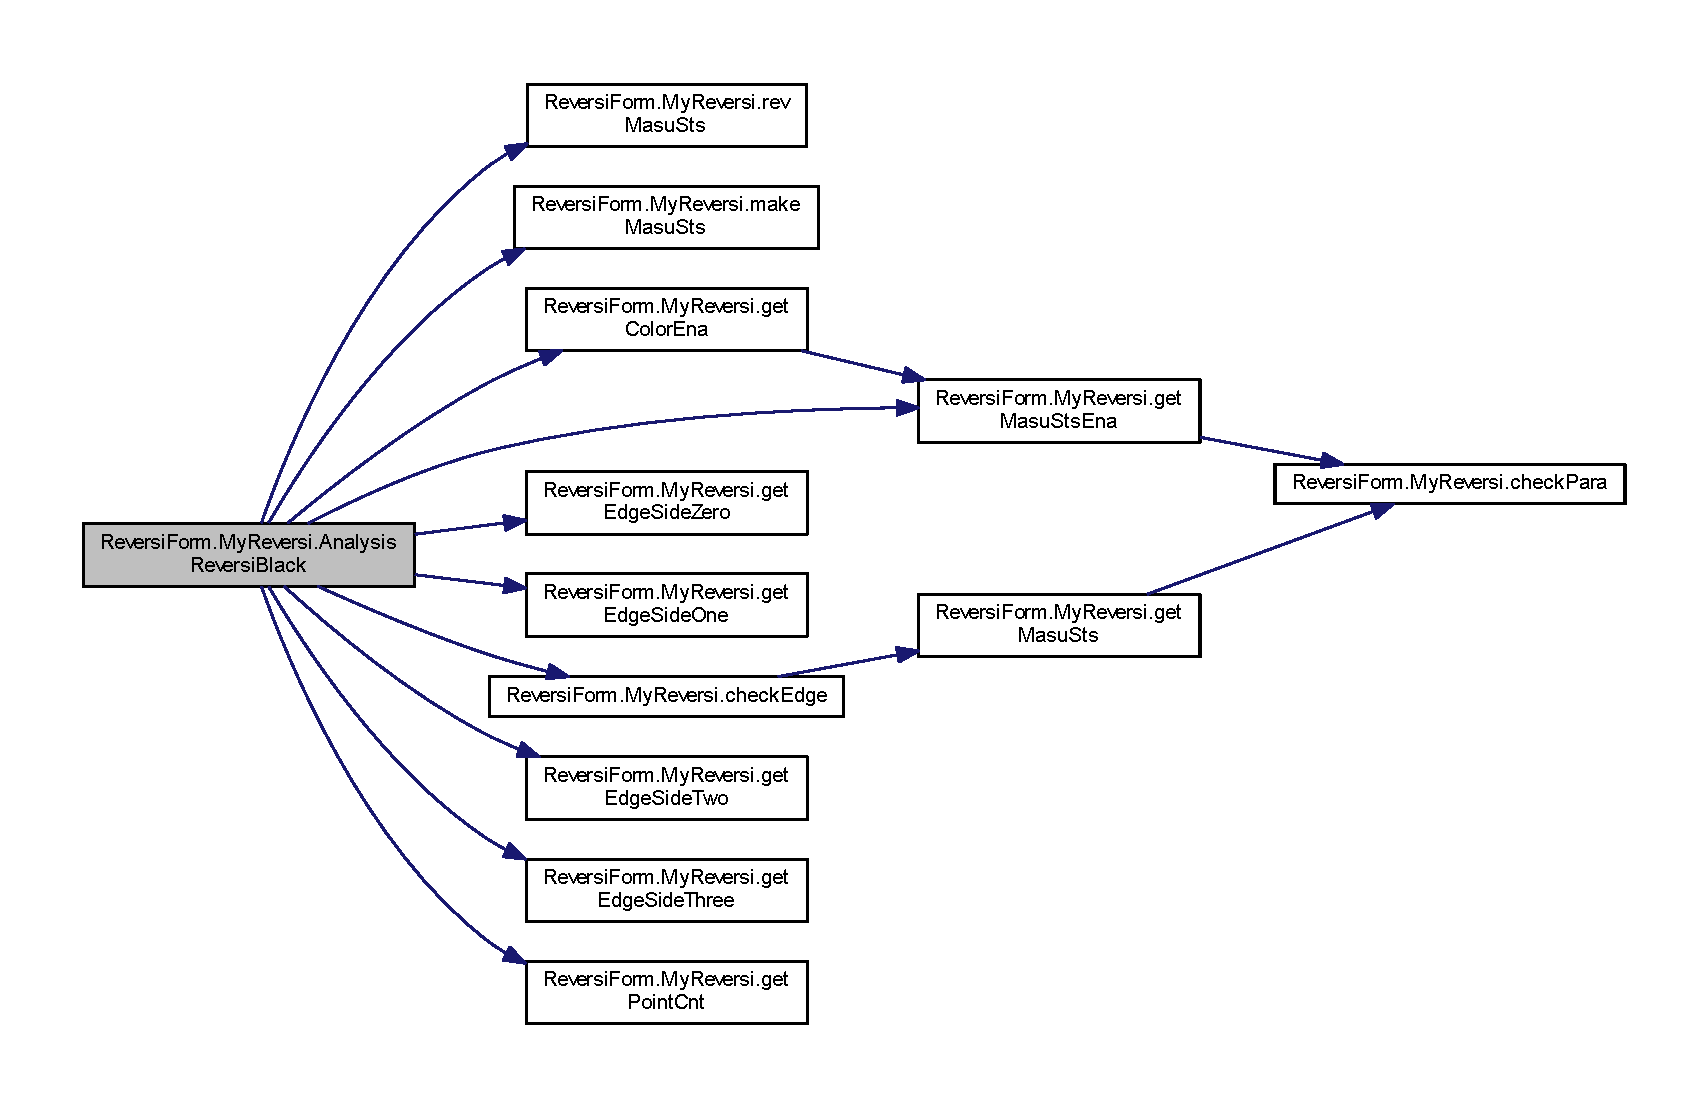
\includegraphics[width=350pt]{class_reversi_form_1_1_my_reversi_adfa9fda128ee816da9b32009326c5a15_cgraph}
\end{center}
\end{figure}
Here is the caller graph for this function\+:
\nopagebreak
\begin{figure}[H]
\begin{center}
\leavevmode
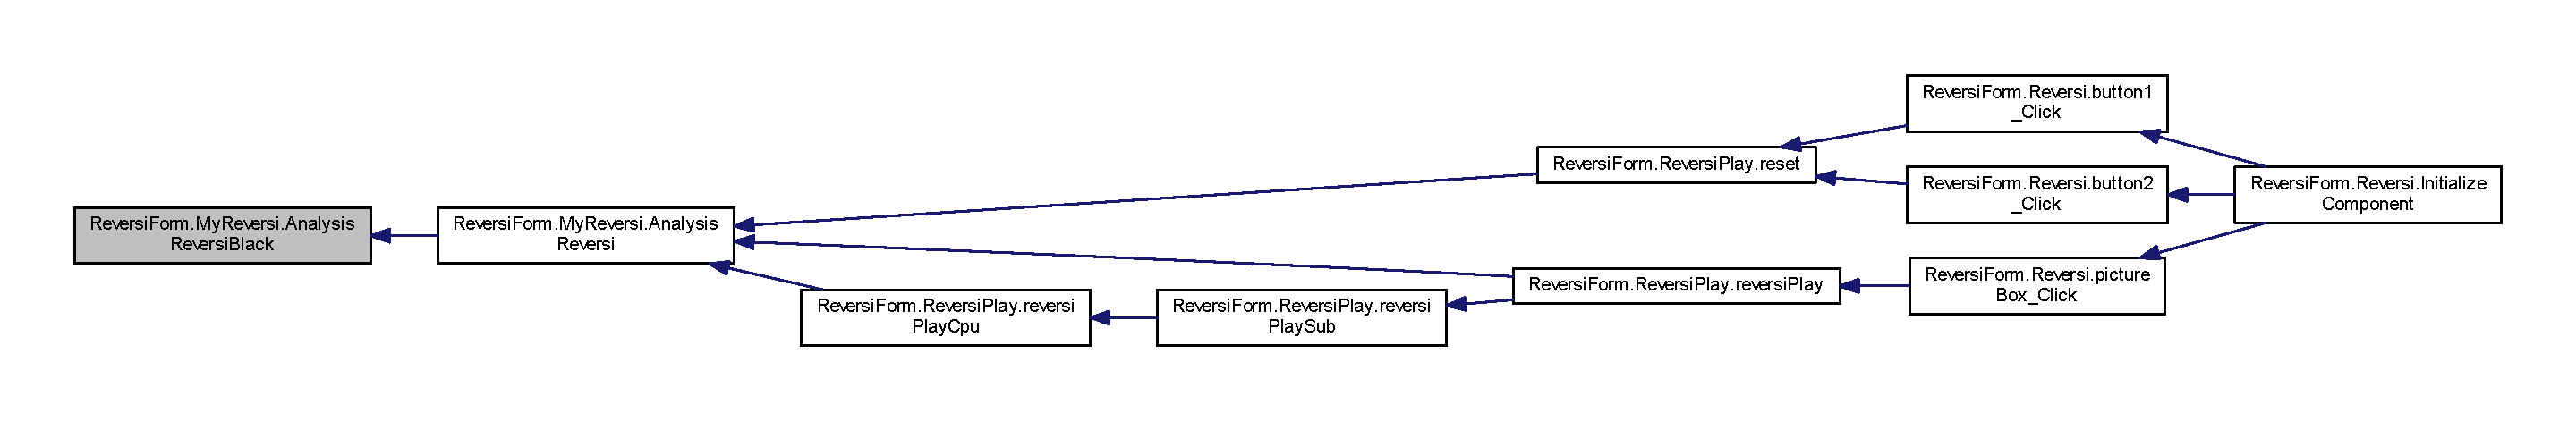
\includegraphics[width=350pt]{class_reversi_form_1_1_my_reversi_adfa9fda128ee816da9b32009326c5a15_icgraph}
\end{center}
\end{figure}
\mbox{\Hypertarget{class_reversi_form_1_1_my_reversi_a2fac17b7121d91063e2d759487f1ed18}\label{class_reversi_form_1_1_my_reversi_a2fac17b7121d91063e2d759487f1ed18}} 
\index{Reversi\+Form\+::\+My\+Reversi@{Reversi\+Form\+::\+My\+Reversi}!Analysis\+Reversi\+White@{Analysis\+Reversi\+White}}
\index{Analysis\+Reversi\+White@{Analysis\+Reversi\+White}!Reversi\+Form\+::\+My\+Reversi@{Reversi\+Form\+::\+My\+Reversi}}
\subsubsection{\texorpdfstring{Analysis\+Reversi\+White()}{AnalysisReversiWhite()}}
{\footnotesize\ttfamily void Reversi\+Form.\+My\+Reversi.\+Analysis\+Reversi\+White (\begin{DoxyParamCaption}{ }\end{DoxyParamCaption})\hspace{0.3cm}{\ttfamily [private]}}



解析を行う(白) 

\begin{DoxyReturn}{Returns}
ありません 
\end{DoxyReturn}
\begin{DoxyAuthor}{Author}
Yuta Yoshinaga 
\end{DoxyAuthor}
\begin{DoxyDate}{Date}
2017.\+10.\+20 
\end{DoxyDate}


Definition at line 808 of file My\+Reversi.\+cs.



Referenced by Reversi\+Form.\+My\+Reversi.\+Analysis\+Reversi().

Here is the call graph for this function\+:
\nopagebreak
\begin{figure}[H]
\begin{center}
\leavevmode
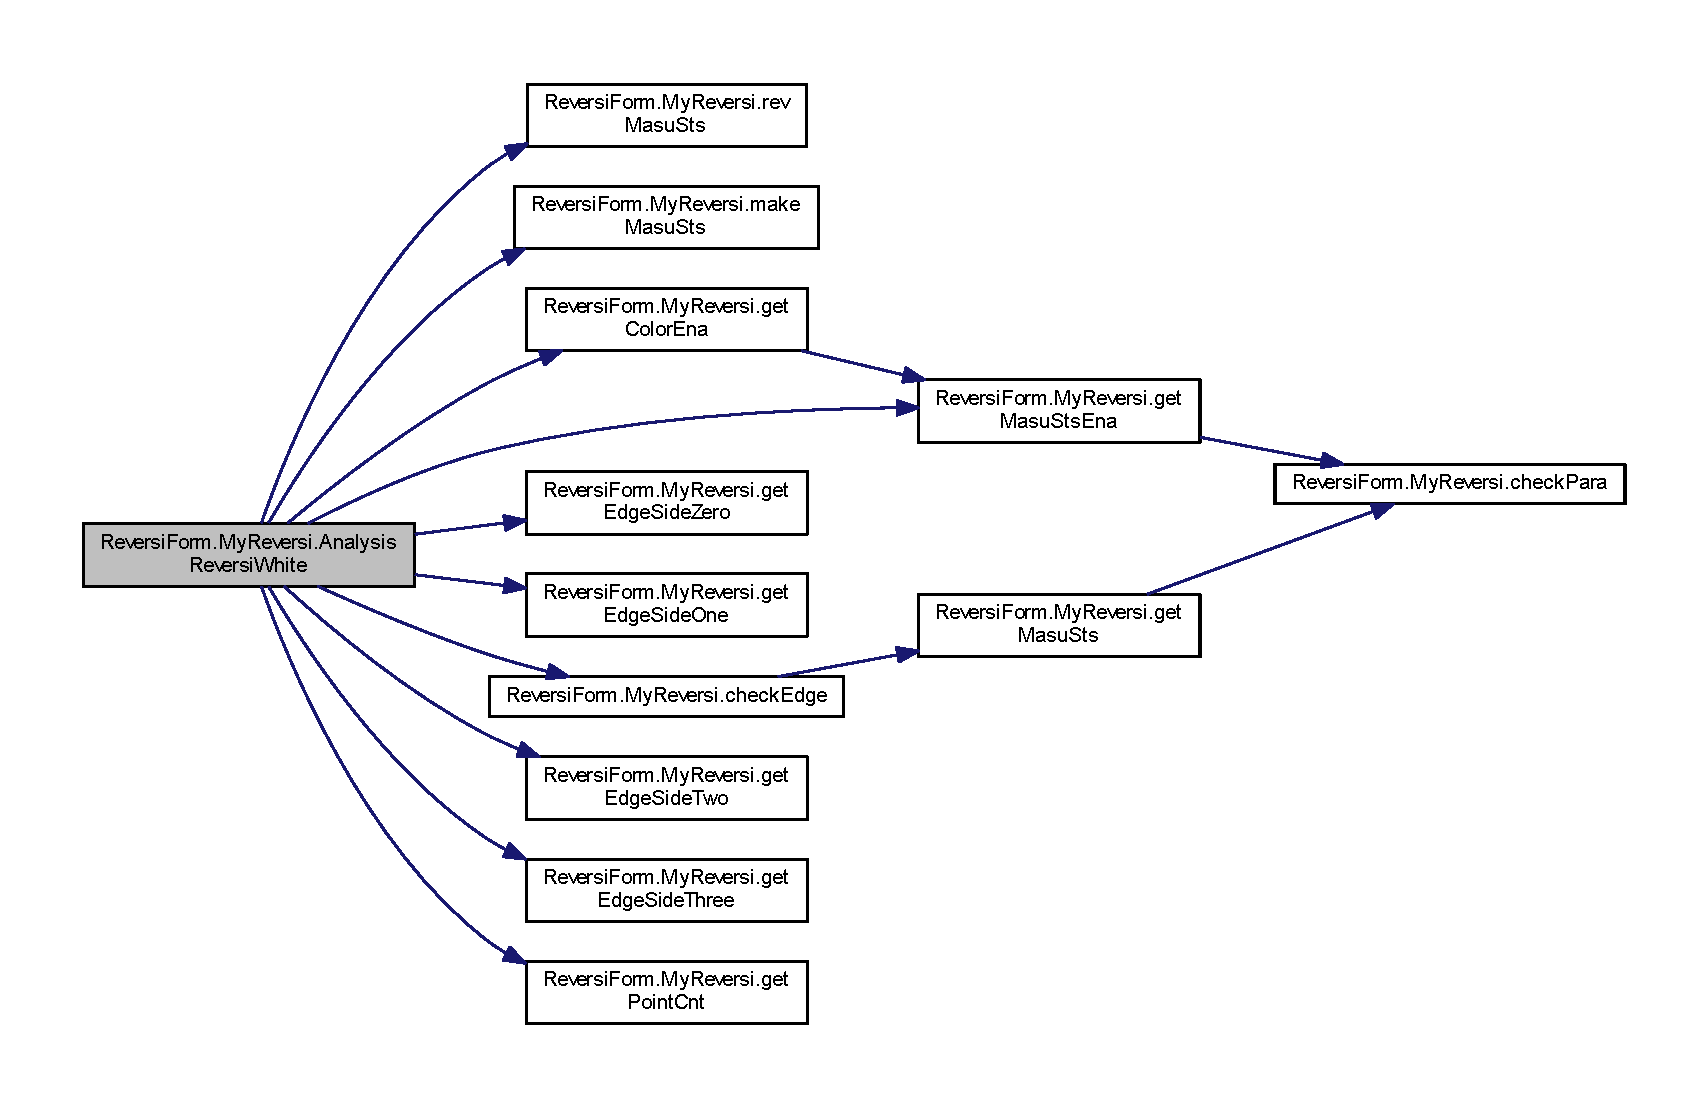
\includegraphics[width=350pt]{class_reversi_form_1_1_my_reversi_a2fac17b7121d91063e2d759487f1ed18_cgraph}
\end{center}
\end{figure}
Here is the caller graph for this function\+:
\nopagebreak
\begin{figure}[H]
\begin{center}
\leavevmode
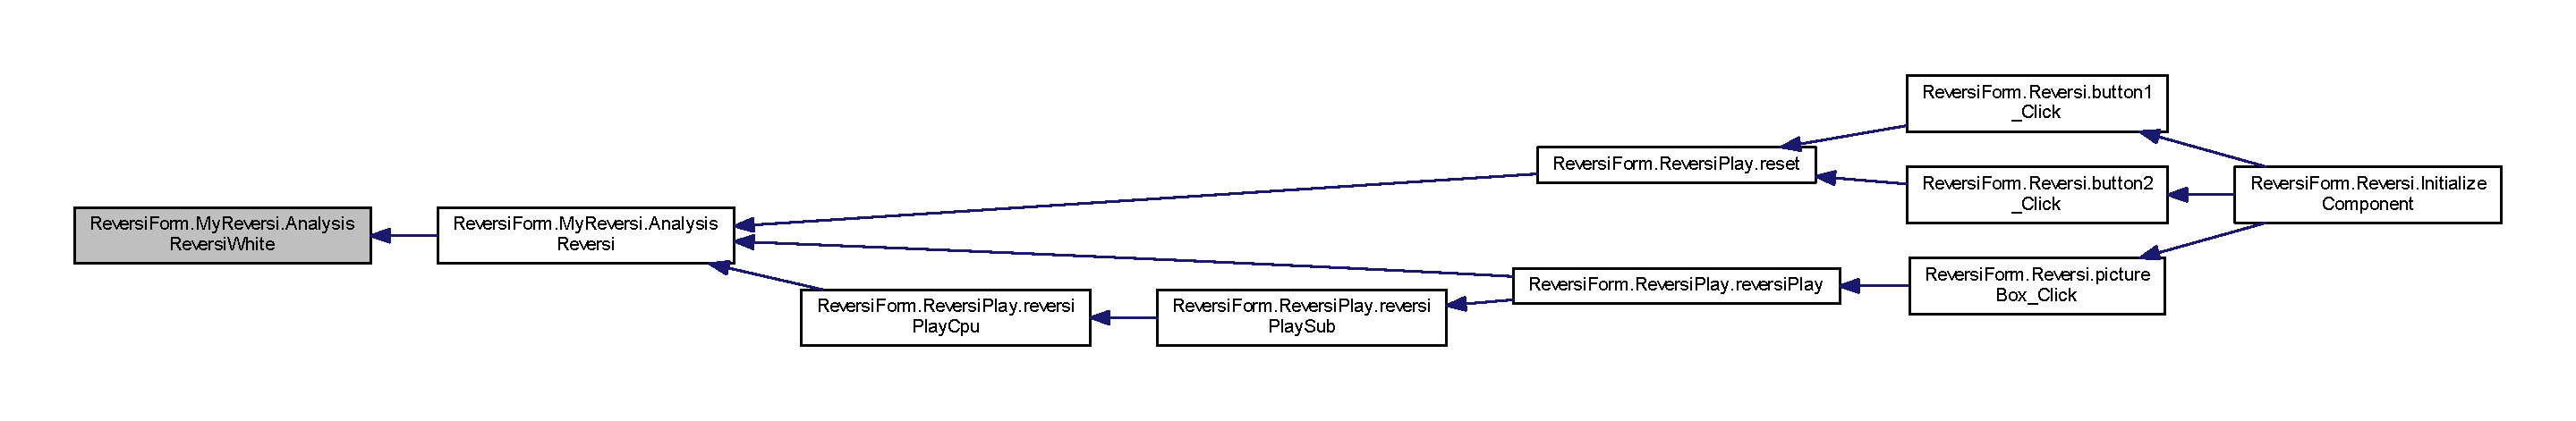
\includegraphics[width=350pt]{class_reversi_form_1_1_my_reversi_a2fac17b7121d91063e2d759487f1ed18_icgraph}
\end{center}
\end{figure}
\mbox{\Hypertarget{class_reversi_form_1_1_my_reversi_aa626cbf9735559841662c8fc413abb98}\label{class_reversi_form_1_1_my_reversi_aa626cbf9735559841662c8fc413abb98}} 
\index{Reversi\+Form\+::\+My\+Reversi@{Reversi\+Form\+::\+My\+Reversi}!check\+Edge@{check\+Edge}}
\index{check\+Edge@{check\+Edge}!Reversi\+Form\+::\+My\+Reversi@{Reversi\+Form\+::\+My\+Reversi}}
\subsubsection{\texorpdfstring{check\+Edge()}{checkEdge()}}
{\footnotesize\ttfamily int Reversi\+Form.\+My\+Reversi.\+check\+Edge (\begin{DoxyParamCaption}\item[{int}]{color,  }\item[{int}]{y,  }\item[{int}]{x }\end{DoxyParamCaption})}



角の隣に置いても角を取られないマス検索 


\begin{DoxyParams}[1]{Parameters}
\mbox{\tt in}  & {\em int} & color コマ色 \\
\hline
\mbox{\tt in}  & {\em int} & y マスの\+Y座標 \\
\hline
\mbox{\tt in}  & {\em int} & x マスの\+X座標 \\
\hline
\end{DoxyParams}
\begin{DoxyReturn}{Returns}
0 \+: 取られる それ以外 \+: 取られない 
\end{DoxyReturn}
\begin{DoxyAuthor}{Author}
Yuta Yoshinaga 
\end{DoxyAuthor}
\begin{DoxyDate}{Date}
2017.\+10.\+20 
\end{DoxyDate}


Definition at line 1312 of file My\+Reversi.\+cs.



Referenced by Reversi\+Form.\+My\+Reversi.\+Analysis\+Reversi\+Black(), Reversi\+Form.\+My\+Reversi.\+Analysis\+Reversi\+White(), and Reversi\+Form.\+Reversi\+Play.\+reversi\+Play\+Cpu().

Here is the call graph for this function\+:
\nopagebreak
\begin{figure}[H]
\begin{center}
\leavevmode
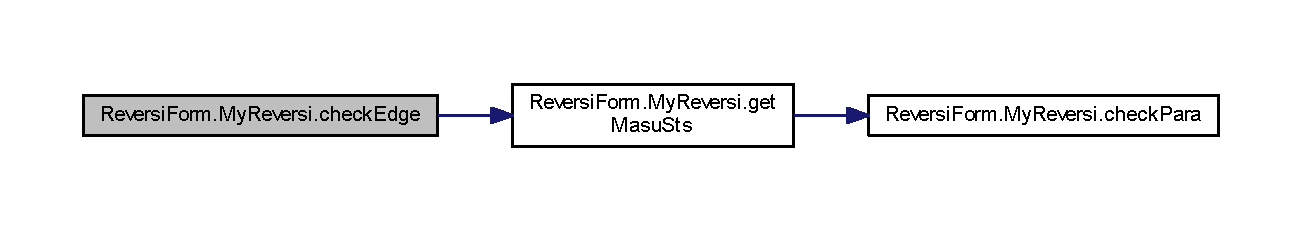
\includegraphics[width=350pt]{class_reversi_form_1_1_my_reversi_aa626cbf9735559841662c8fc413abb98_cgraph}
\end{center}
\end{figure}
Here is the caller graph for this function\+:
\nopagebreak
\begin{figure}[H]
\begin{center}
\leavevmode
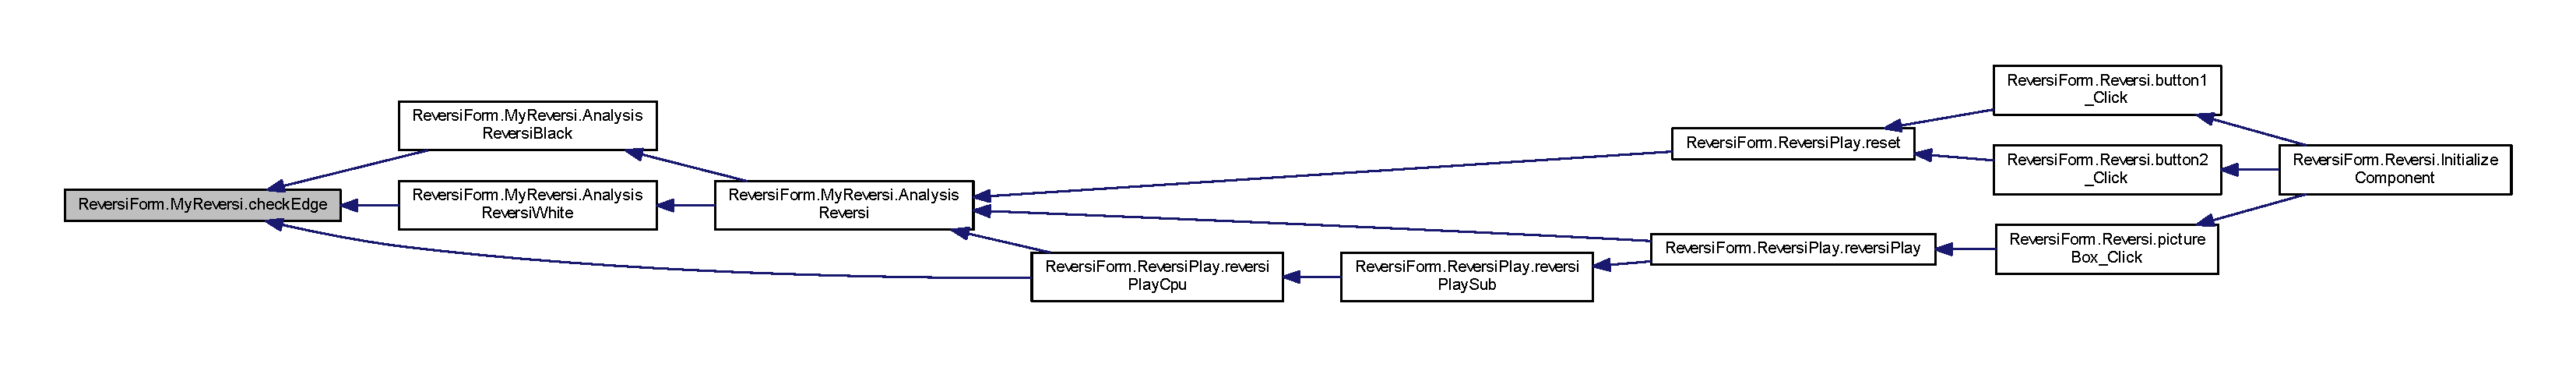
\includegraphics[width=350pt]{class_reversi_form_1_1_my_reversi_aa626cbf9735559841662c8fc413abb98_icgraph}
\end{center}
\end{figure}
\mbox{\Hypertarget{class_reversi_form_1_1_my_reversi_a7d861112d0ddeb404cd3e8d8f5c2756b}\label{class_reversi_form_1_1_my_reversi_a7d861112d0ddeb404cd3e8d8f5c2756b}} 
\index{Reversi\+Form\+::\+My\+Reversi@{Reversi\+Form\+::\+My\+Reversi}!check\+Para@{check\+Para}}
\index{check\+Para@{check\+Para}!Reversi\+Form\+::\+My\+Reversi@{Reversi\+Form\+::\+My\+Reversi}}
\subsubsection{\texorpdfstring{check\+Para()}{checkPara()}}
{\footnotesize\ttfamily int Reversi\+Form.\+My\+Reversi.\+check\+Para (\begin{DoxyParamCaption}\item[{int}]{para,  }\item[{int}]{min,  }\item[{int}]{max }\end{DoxyParamCaption})\hspace{0.3cm}{\ttfamily [private]}}



パラメーター範囲チェック 


\begin{DoxyParams}[1]{Parameters}
\mbox{\tt in}  & {\em int} & para チェックパラメーター \\
\hline
\mbox{\tt in}  & {\em int} & min パラメーター最小値 \\
\hline
\mbox{\tt in}  & {\em int} & max パラメーター最大値 \\
\hline
\end{DoxyParams}
\begin{DoxyReturn}{Returns}
0 \+: 成功 それ以外 \+: 失敗 
\end{DoxyReturn}
\begin{DoxyAuthor}{Author}
Yuta Yoshinaga 
\end{DoxyAuthor}
\begin{DoxyDate}{Date}
2017.\+10.\+20 
\end{DoxyDate}


Definition at line 655 of file My\+Reversi.\+cs.



Referenced by Reversi\+Form.\+My\+Reversi.\+get\+History(), Reversi\+Form.\+My\+Reversi.\+get\+Masu\+Sts(), Reversi\+Form.\+My\+Reversi.\+get\+Masu\+Sts\+Cnt(), Reversi\+Form.\+My\+Reversi.\+get\+Masu\+Sts\+Ena(), Reversi\+Form.\+My\+Reversi.\+get\+Masu\+Sts\+Old(), Reversi\+Form.\+My\+Reversi.\+get\+Pass\+Ena(), Reversi\+Form.\+My\+Reversi.\+get\+Point(), Reversi\+Form.\+My\+Reversi.\+get\+Point\+Anz(), and Reversi\+Form.\+My\+Reversi.\+set\+Masu\+Cnt().

Here is the caller graph for this function\+:
\nopagebreak
\begin{figure}[H]
\begin{center}
\leavevmode
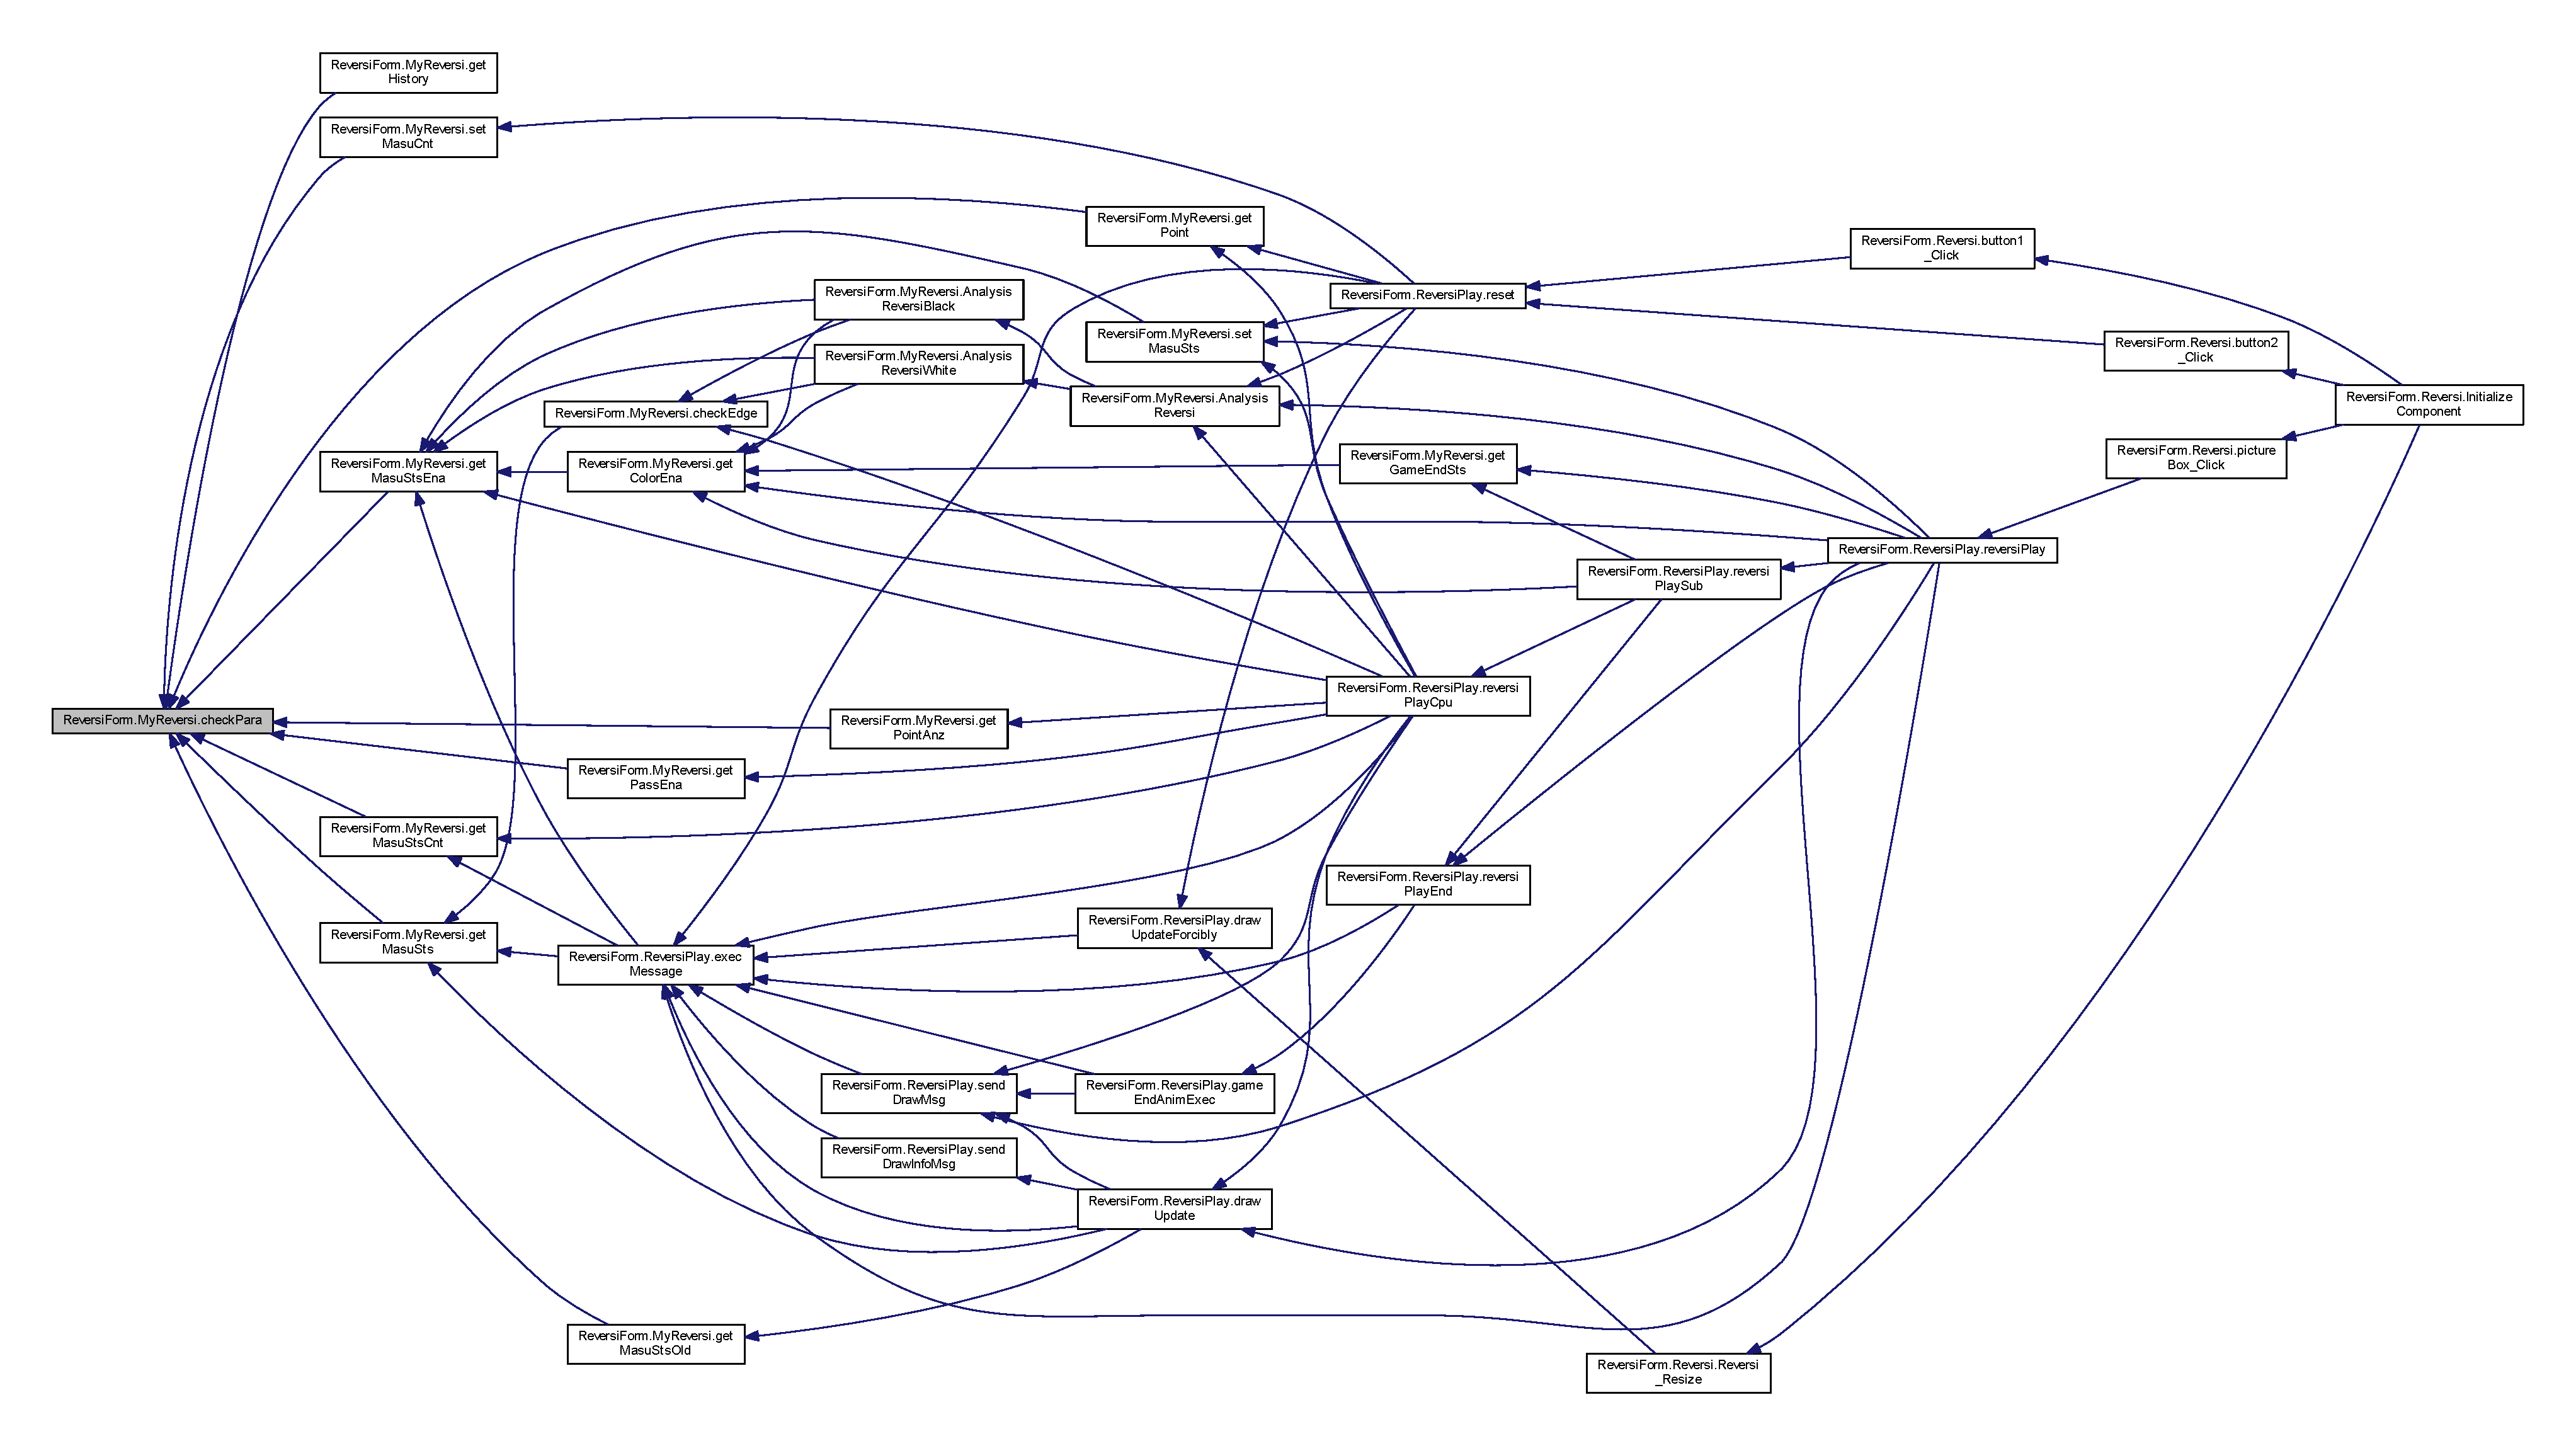
\includegraphics[width=350pt]{class_reversi_form_1_1_my_reversi_a7d861112d0ddeb404cd3e8d8f5c2756b_icgraph}
\end{center}
\end{figure}
\mbox{\Hypertarget{class_reversi_form_1_1_my_reversi_aa340f79c0f7bb78750c410ce73ca7b99}\label{class_reversi_form_1_1_my_reversi_aa340f79c0f7bb78750c410ce73ca7b99}} 
\index{Reversi\+Form\+::\+My\+Reversi@{Reversi\+Form\+::\+My\+Reversi}!Clone@{Clone}}
\index{Clone@{Clone}!Reversi\+Form\+::\+My\+Reversi@{Reversi\+Form\+::\+My\+Reversi}}
\subsubsection{\texorpdfstring{Clone()}{Clone()}}
{\footnotesize\ttfamily \hyperlink{class_reversi_form_1_1_my_reversi}{My\+Reversi} Reversi\+Form.\+My\+Reversi.\+Clone (\begin{DoxyParamCaption}{ }\end{DoxyParamCaption})}



コピー 

\begin{DoxyReturn}{Returns}
オブジェクトコピー 
\end{DoxyReturn}
\begin{DoxyAuthor}{Author}
Yuta Yoshinaga 
\end{DoxyAuthor}
\begin{DoxyDate}{Date}
2017.\+10.\+20 
\end{DoxyDate}


Definition at line 230 of file My\+Reversi.\+cs.

\mbox{\Hypertarget{class_reversi_form_1_1_my_reversi_aa69640136727deb89addafae8e8e54cb}\label{class_reversi_form_1_1_my_reversi_aa69640136727deb89addafae8e8e54cb}} 
\index{Reversi\+Form\+::\+My\+Reversi@{Reversi\+Form\+::\+My\+Reversi}!get\+Bet\+Cnt@{get\+Bet\+Cnt}}
\index{get\+Bet\+Cnt@{get\+Bet\+Cnt}!Reversi\+Form\+::\+My\+Reversi@{Reversi\+Form\+::\+My\+Reversi}}
\subsubsection{\texorpdfstring{get\+Bet\+Cnt()}{getBetCnt()}}
{\footnotesize\ttfamily int Reversi\+Form.\+My\+Reversi.\+get\+Bet\+Cnt (\begin{DoxyParamCaption}\item[{int}]{color }\end{DoxyParamCaption})}



コマ数取得 


\begin{DoxyParams}[1]{Parameters}
\mbox{\tt in}  & {\em int} & color コマ色 \\
\hline
\end{DoxyParams}
\begin{DoxyReturn}{Returns}
コマ数取得 
\end{DoxyReturn}
\begin{DoxyAuthor}{Author}
Yuta Yoshinaga 
\end{DoxyAuthor}
\begin{DoxyDate}{Date}
2017.\+10.\+20 
\end{DoxyDate}


Definition at line 1215 of file My\+Reversi.\+cs.



Referenced by Reversi\+Form.\+Reversi\+Play.\+exec\+Message(), Reversi\+Form.\+Reversi\+Play.\+game\+End\+Anim\+Exec(), Reversi\+Form.\+Reversi\+Play.\+reversi\+Play\+Cpu(), and Reversi\+Form.\+Reversi\+Play.\+reversi\+Play\+End().

Here is the caller graph for this function\+:
\nopagebreak
\begin{figure}[H]
\begin{center}
\leavevmode
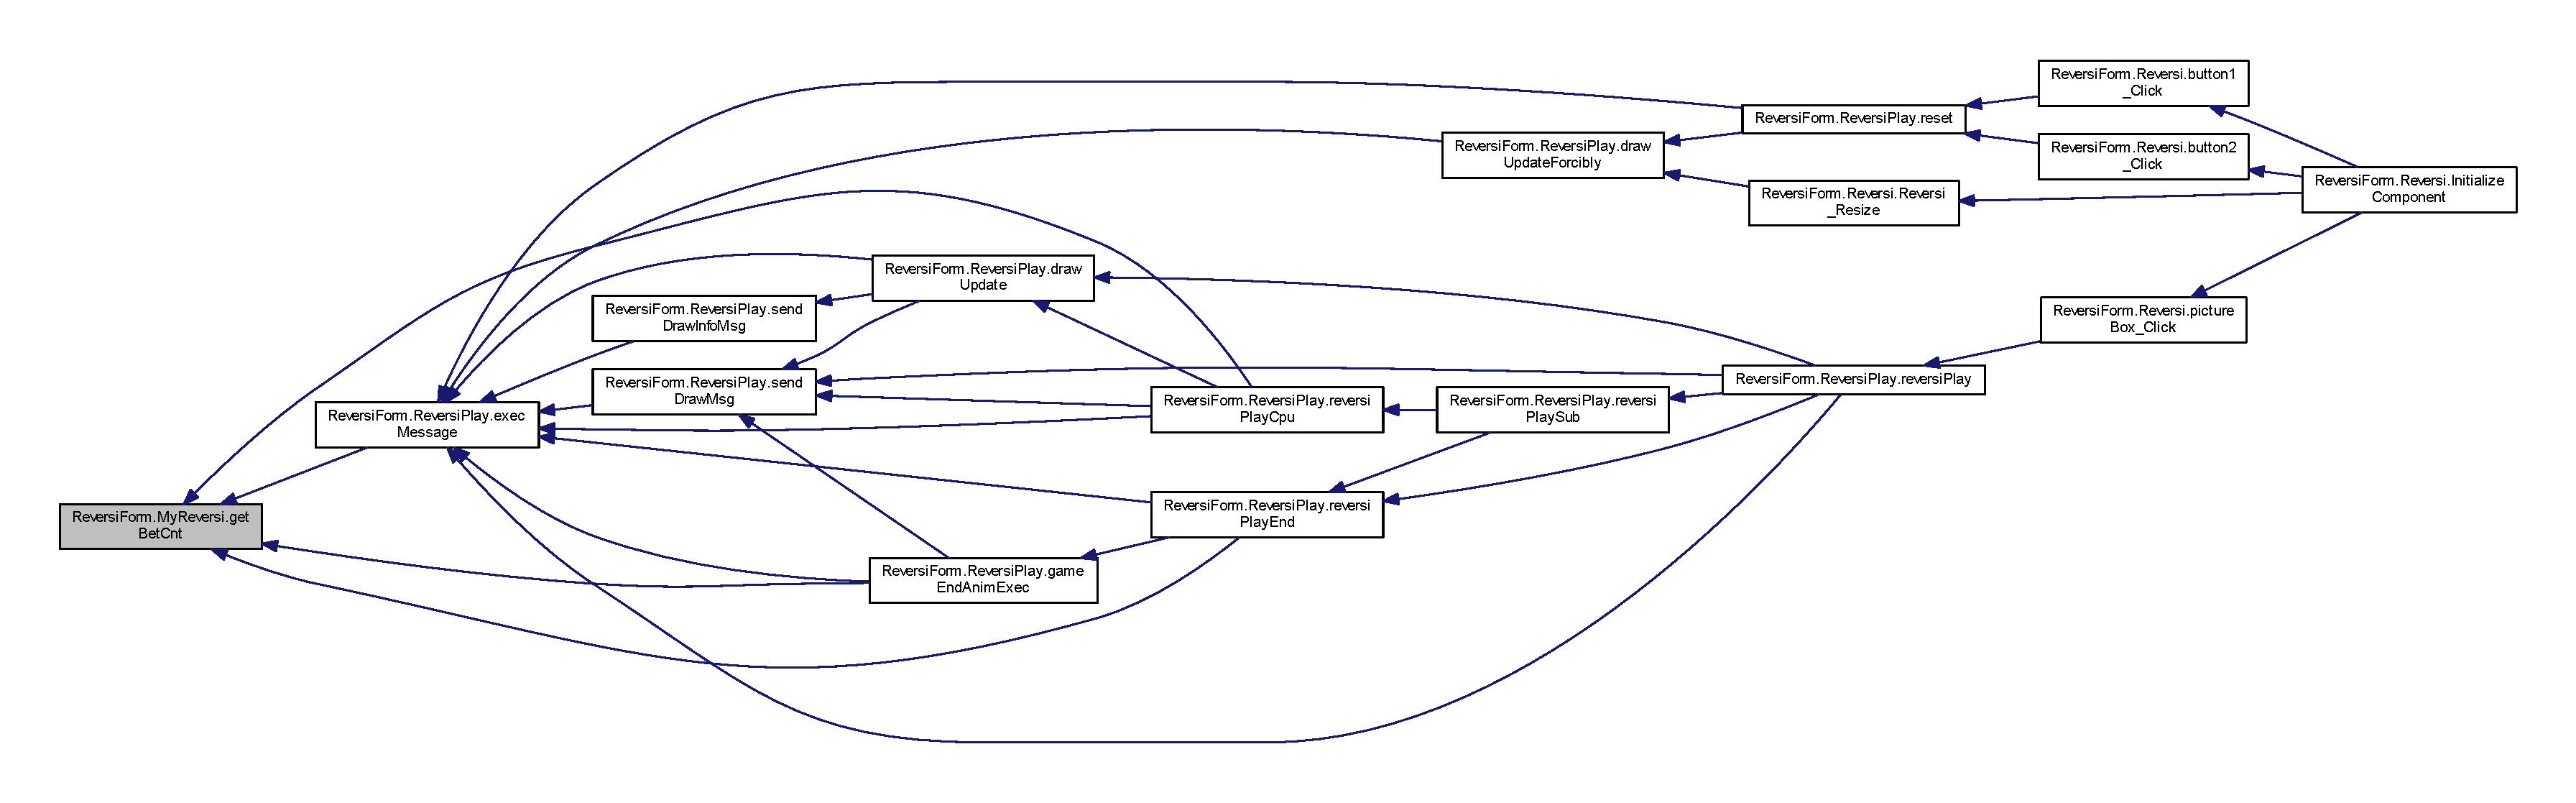
\includegraphics[width=350pt]{class_reversi_form_1_1_my_reversi_aa69640136727deb89addafae8e8e54cb_icgraph}
\end{center}
\end{figure}
\mbox{\Hypertarget{class_reversi_form_1_1_my_reversi_a960e2691d2d106e5ad6036cfe9cf2503}\label{class_reversi_form_1_1_my_reversi_a960e2691d2d106e5ad6036cfe9cf2503}} 
\index{Reversi\+Form\+::\+My\+Reversi@{Reversi\+Form\+::\+My\+Reversi}!get\+Color\+Ena@{get\+Color\+Ena}}
\index{get\+Color\+Ena@{get\+Color\+Ena}!Reversi\+Form\+::\+My\+Reversi@{Reversi\+Form\+::\+My\+Reversi}}
\subsubsection{\texorpdfstring{get\+Color\+Ena()}{getColorEna()}}
{\footnotesize\ttfamily int Reversi\+Form.\+My\+Reversi.\+get\+Color\+Ena (\begin{DoxyParamCaption}\item[{int}]{color }\end{DoxyParamCaption})}



指定色が現在置ける場所があるかチェック 


\begin{DoxyParams}[1]{Parameters}
\mbox{\tt in}  & {\em int} & color コマ色 \\
\hline
\end{DoxyParams}
\begin{DoxyReturn}{Returns}
0 \+: 成功 それ以外 \+: 失敗 
\end{DoxyReturn}
\begin{DoxyAuthor}{Author}
Yuta Yoshinaga 
\end{DoxyAuthor}
\begin{DoxyDate}{Date}
2017.\+10.\+20 
\end{DoxyDate}


Definition at line 1063 of file My\+Reversi.\+cs.



Referenced by Reversi\+Form.\+My\+Reversi.\+Analysis\+Reversi\+Black(), Reversi\+Form.\+My\+Reversi.\+Analysis\+Reversi\+White(), Reversi\+Form.\+My\+Reversi.\+get\+Game\+End\+Sts(), Reversi\+Form.\+Reversi\+Play.\+reversi\+Play(), and Reversi\+Form.\+Reversi\+Play.\+reversi\+Play\+Sub().

Here is the call graph for this function\+:
\nopagebreak
\begin{figure}[H]
\begin{center}
\leavevmode
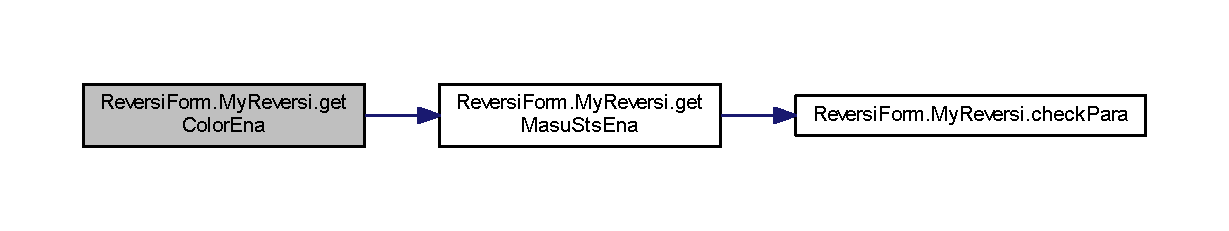
\includegraphics[width=350pt]{class_reversi_form_1_1_my_reversi_a960e2691d2d106e5ad6036cfe9cf2503_cgraph}
\end{center}
\end{figure}
Here is the caller graph for this function\+:
\nopagebreak
\begin{figure}[H]
\begin{center}
\leavevmode
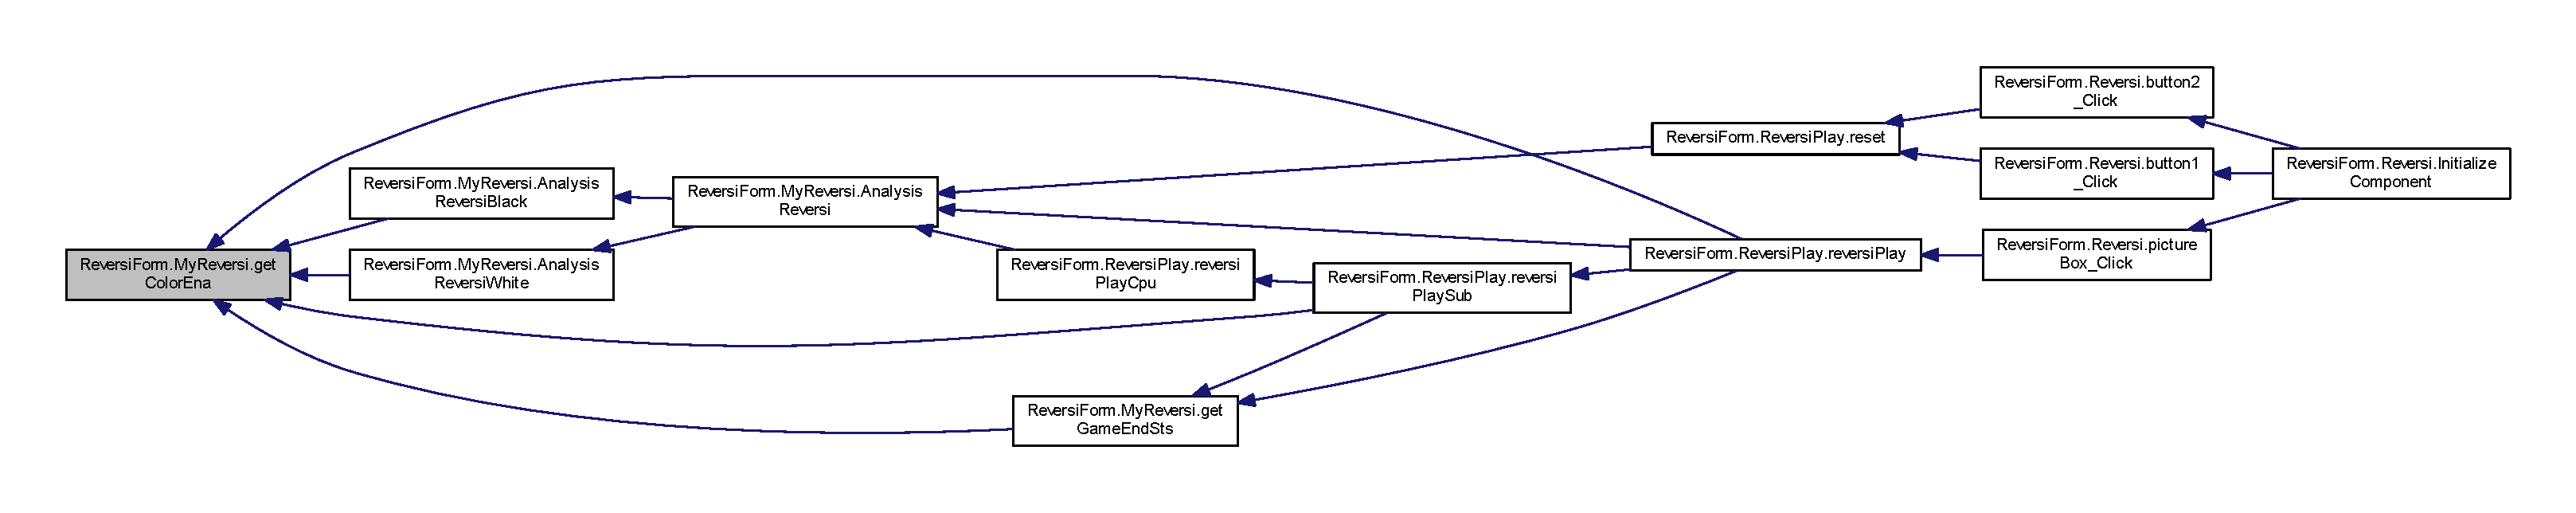
\includegraphics[width=350pt]{class_reversi_form_1_1_my_reversi_a960e2691d2d106e5ad6036cfe9cf2503_icgraph}
\end{center}
\end{figure}
\mbox{\Hypertarget{class_reversi_form_1_1_my_reversi_a998eeefb18faecad172a6e1da4c70d7c}\label{class_reversi_form_1_1_my_reversi_a998eeefb18faecad172a6e1da4c70d7c}} 
\index{Reversi\+Form\+::\+My\+Reversi@{Reversi\+Form\+::\+My\+Reversi}!get\+Edge\+Side\+One@{get\+Edge\+Side\+One}}
\index{get\+Edge\+Side\+One@{get\+Edge\+Side\+One}!Reversi\+Form\+::\+My\+Reversi@{Reversi\+Form\+::\+My\+Reversi}}
\subsubsection{\texorpdfstring{get\+Edge\+Side\+One()}{getEdgeSideOne()}}
{\footnotesize\ttfamily int Reversi\+Form.\+My\+Reversi.\+get\+Edge\+Side\+One (\begin{DoxyParamCaption}\item[{int}]{y,  }\item[{int}]{x }\end{DoxyParamCaption})}



指定座標が角の一つ手前か取得 


\begin{DoxyParams}[1]{Parameters}
\mbox{\tt in}  & {\em int} & y Y座標 \\
\hline
\mbox{\tt in}  & {\em int} & x X座標 \\
\hline
\end{DoxyParams}
\begin{DoxyReturn}{Returns}
0 \+: 成功 それ以外 \+: 失敗 
\end{DoxyReturn}
\begin{DoxyAuthor}{Author}
Yuta Yoshinaga 
\end{DoxyAuthor}
\begin{DoxyDate}{Date}
2017.\+10.\+20 
\end{DoxyDate}


Definition at line 1454 of file My\+Reversi.\+cs.



Referenced by Reversi\+Form.\+My\+Reversi.\+Analysis\+Reversi\+Black(), Reversi\+Form.\+My\+Reversi.\+Analysis\+Reversi\+White(), and Reversi\+Form.\+Reversi\+Play.\+reversi\+Play\+Cpu().

Here is the caller graph for this function\+:
\nopagebreak
\begin{figure}[H]
\begin{center}
\leavevmode
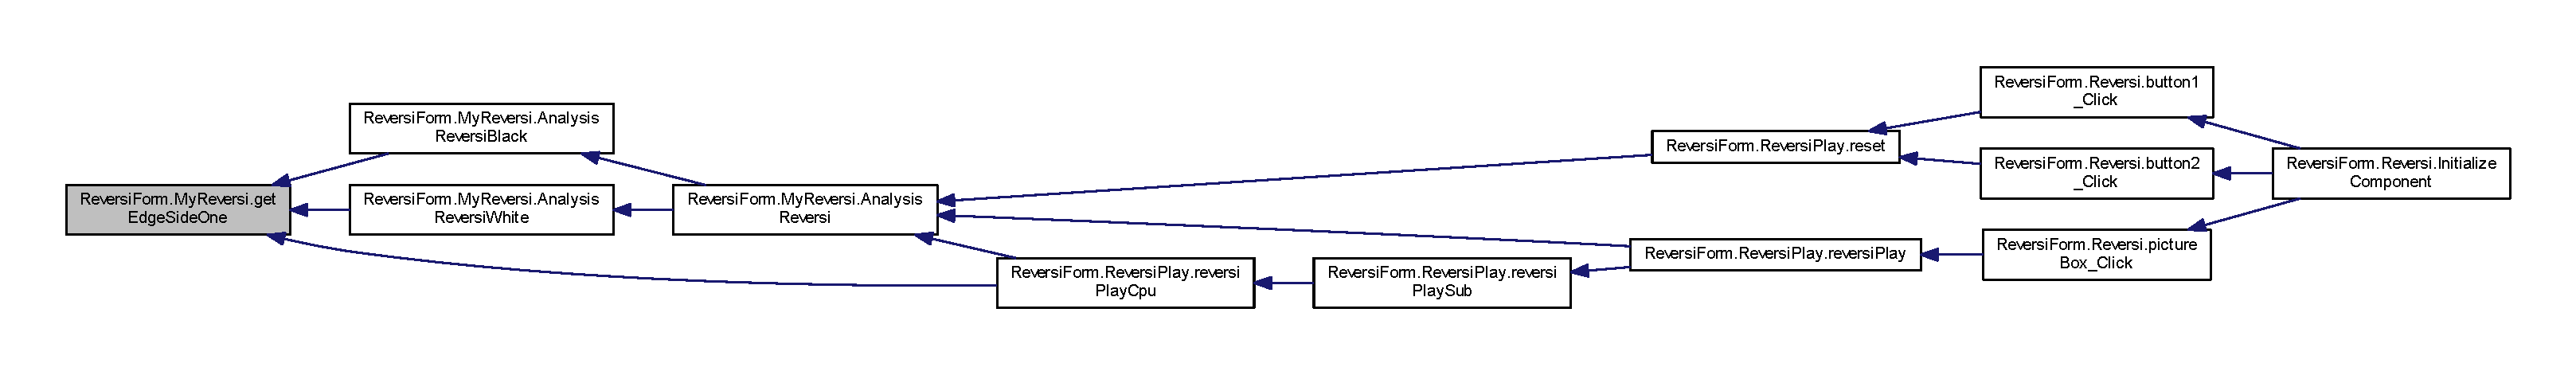
\includegraphics[width=350pt]{class_reversi_form_1_1_my_reversi_a998eeefb18faecad172a6e1da4c70d7c_icgraph}
\end{center}
\end{figure}
\mbox{\Hypertarget{class_reversi_form_1_1_my_reversi_af6fee61bda5532c4c130e5660f7ce66f}\label{class_reversi_form_1_1_my_reversi_af6fee61bda5532c4c130e5660f7ce66f}} 
\index{Reversi\+Form\+::\+My\+Reversi@{Reversi\+Form\+::\+My\+Reversi}!get\+Edge\+Side\+Three@{get\+Edge\+Side\+Three}}
\index{get\+Edge\+Side\+Three@{get\+Edge\+Side\+Three}!Reversi\+Form\+::\+My\+Reversi@{Reversi\+Form\+::\+My\+Reversi}}
\subsubsection{\texorpdfstring{get\+Edge\+Side\+Three()}{getEdgeSideThree()}}
{\footnotesize\ttfamily int Reversi\+Form.\+My\+Reversi.\+get\+Edge\+Side\+Three (\begin{DoxyParamCaption}\item[{int}]{y,  }\item[{int}]{x }\end{DoxyParamCaption})}



指定座標が角の三つ以上手前か取得 


\begin{DoxyParams}[1]{Parameters}
\mbox{\tt in}  & {\em int} & y Y座標 \\
\hline
\mbox{\tt in}  & {\em int} & x X座標 \\
\hline
\end{DoxyParams}
\begin{DoxyReturn}{Returns}
0 \+: 成功 それ以外 \+: 失敗 
\end{DoxyReturn}
\begin{DoxyAuthor}{Author}
Yuta Yoshinaga 
\end{DoxyAuthor}
\begin{DoxyDate}{Date}
2017.\+10.\+20 
\end{DoxyDate}


Definition at line 1518 of file My\+Reversi.\+cs.



Referenced by Reversi\+Form.\+My\+Reversi.\+Analysis\+Reversi\+Black(), Reversi\+Form.\+My\+Reversi.\+Analysis\+Reversi\+White(), and Reversi\+Form.\+Reversi\+Play.\+reversi\+Play\+Cpu().

Here is the caller graph for this function\+:
\nopagebreak
\begin{figure}[H]
\begin{center}
\leavevmode
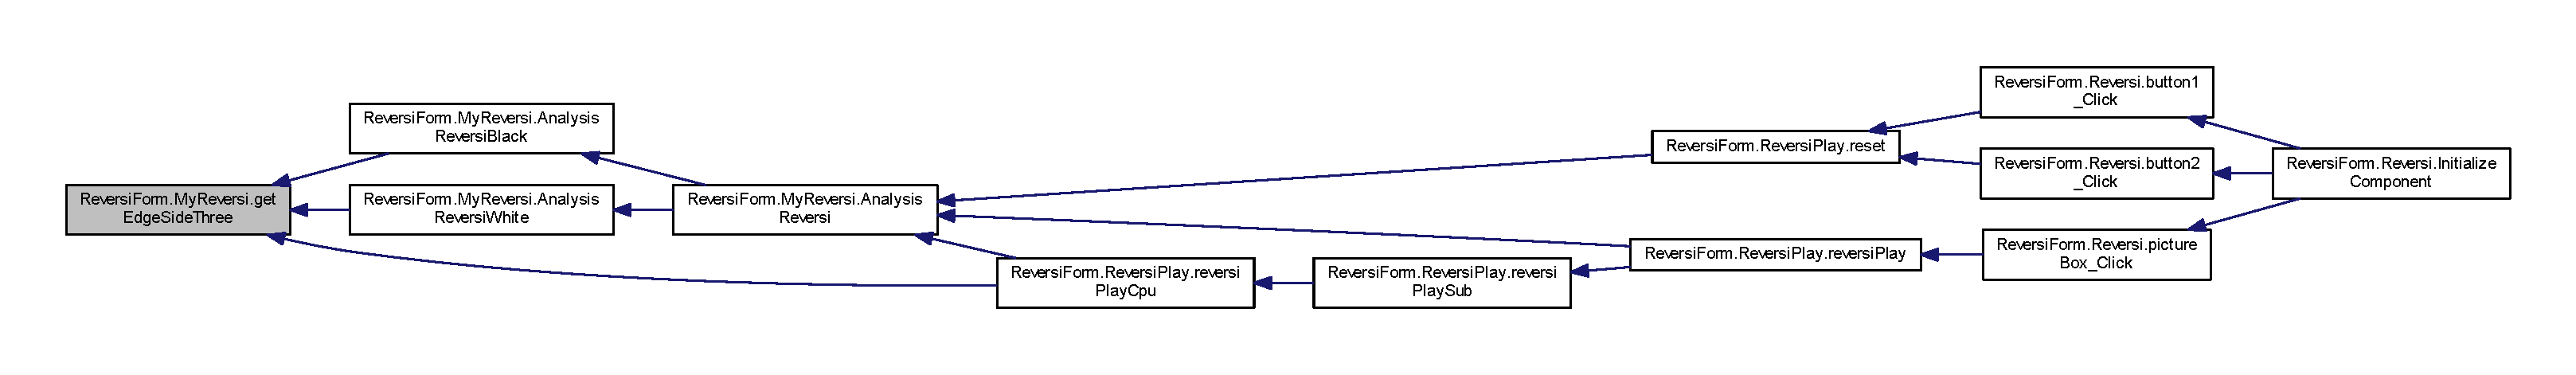
\includegraphics[width=350pt]{class_reversi_form_1_1_my_reversi_af6fee61bda5532c4c130e5660f7ce66f_icgraph}
\end{center}
\end{figure}
\mbox{\Hypertarget{class_reversi_form_1_1_my_reversi_a4b5395df3beb684f55b10bab91661c78}\label{class_reversi_form_1_1_my_reversi_a4b5395df3beb684f55b10bab91661c78}} 
\index{Reversi\+Form\+::\+My\+Reversi@{Reversi\+Form\+::\+My\+Reversi}!get\+Edge\+Side\+Two@{get\+Edge\+Side\+Two}}
\index{get\+Edge\+Side\+Two@{get\+Edge\+Side\+Two}!Reversi\+Form\+::\+My\+Reversi@{Reversi\+Form\+::\+My\+Reversi}}
\subsubsection{\texorpdfstring{get\+Edge\+Side\+Two()}{getEdgeSideTwo()}}
{\footnotesize\ttfamily int Reversi\+Form.\+My\+Reversi.\+get\+Edge\+Side\+Two (\begin{DoxyParamCaption}\item[{int}]{y,  }\item[{int}]{x }\end{DoxyParamCaption})}



指定座標が角の二つ手前か取得 


\begin{DoxyParams}[1]{Parameters}
\mbox{\tt in}  & {\em int} & y Y座標 \\
\hline
\mbox{\tt in}  & {\em int} & x X座標 \\
\hline
\end{DoxyParams}
\begin{DoxyReturn}{Returns}
0 \+: 成功 それ以外 \+: 失敗 
\end{DoxyReturn}
\begin{DoxyAuthor}{Author}
Yuta Yoshinaga 
\end{DoxyAuthor}
\begin{DoxyDate}{Date}
2017.\+10.\+20 
\end{DoxyDate}


Definition at line 1486 of file My\+Reversi.\+cs.



Referenced by Reversi\+Form.\+My\+Reversi.\+Analysis\+Reversi\+Black(), Reversi\+Form.\+My\+Reversi.\+Analysis\+Reversi\+White(), and Reversi\+Form.\+Reversi\+Play.\+reversi\+Play\+Cpu().

Here is the caller graph for this function\+:
\nopagebreak
\begin{figure}[H]
\begin{center}
\leavevmode
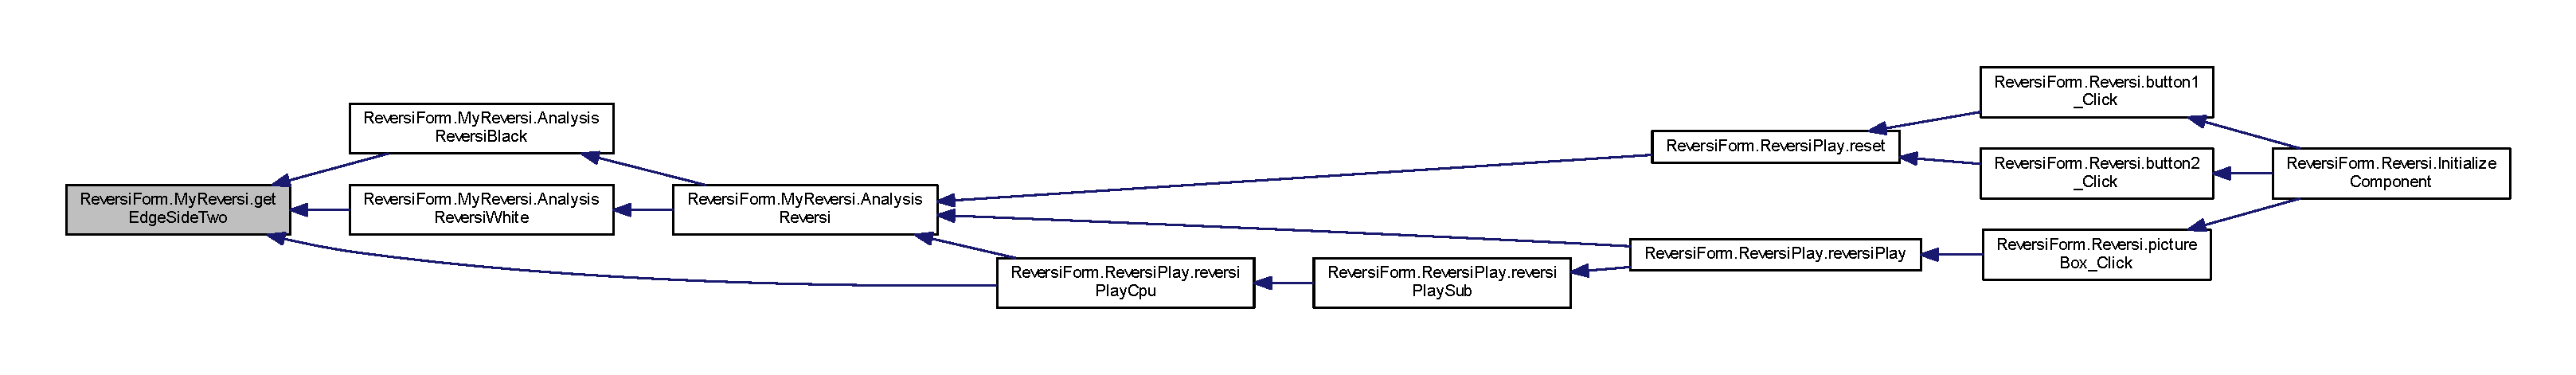
\includegraphics[width=350pt]{class_reversi_form_1_1_my_reversi_a4b5395df3beb684f55b10bab91661c78_icgraph}
\end{center}
\end{figure}
\mbox{\Hypertarget{class_reversi_form_1_1_my_reversi_a64216270f06c7c309d39bfcb681dd1b3}\label{class_reversi_form_1_1_my_reversi_a64216270f06c7c309d39bfcb681dd1b3}} 
\index{Reversi\+Form\+::\+My\+Reversi@{Reversi\+Form\+::\+My\+Reversi}!get\+Edge\+Side\+Zero@{get\+Edge\+Side\+Zero}}
\index{get\+Edge\+Side\+Zero@{get\+Edge\+Side\+Zero}!Reversi\+Form\+::\+My\+Reversi@{Reversi\+Form\+::\+My\+Reversi}}
\subsubsection{\texorpdfstring{get\+Edge\+Side\+Zero()}{getEdgeSideZero()}}
{\footnotesize\ttfamily int Reversi\+Form.\+My\+Reversi.\+get\+Edge\+Side\+Zero (\begin{DoxyParamCaption}\item[{int}]{y,  }\item[{int}]{x }\end{DoxyParamCaption})}



指定座標が角か取得 


\begin{DoxyParams}[1]{Parameters}
\mbox{\tt in}  & {\em int} & y Y座標 \\
\hline
\mbox{\tt in}  & {\em int} & x X座標 \\
\hline
\end{DoxyParams}
\begin{DoxyReturn}{Returns}
0 \+: 成功 それ以外 \+: 失敗 
\end{DoxyReturn}
\begin{DoxyAuthor}{Author}
Yuta Yoshinaga 
\end{DoxyAuthor}
\begin{DoxyDate}{Date}
2017.\+10.\+20 
\end{DoxyDate}


Definition at line 1430 of file My\+Reversi.\+cs.



Referenced by Reversi\+Form.\+My\+Reversi.\+Analysis\+Reversi\+Black(), Reversi\+Form.\+My\+Reversi.\+Analysis\+Reversi\+White(), and Reversi\+Form.\+Reversi\+Play.\+reversi\+Play\+Cpu().

Here is the caller graph for this function\+:
\nopagebreak
\begin{figure}[H]
\begin{center}
\leavevmode
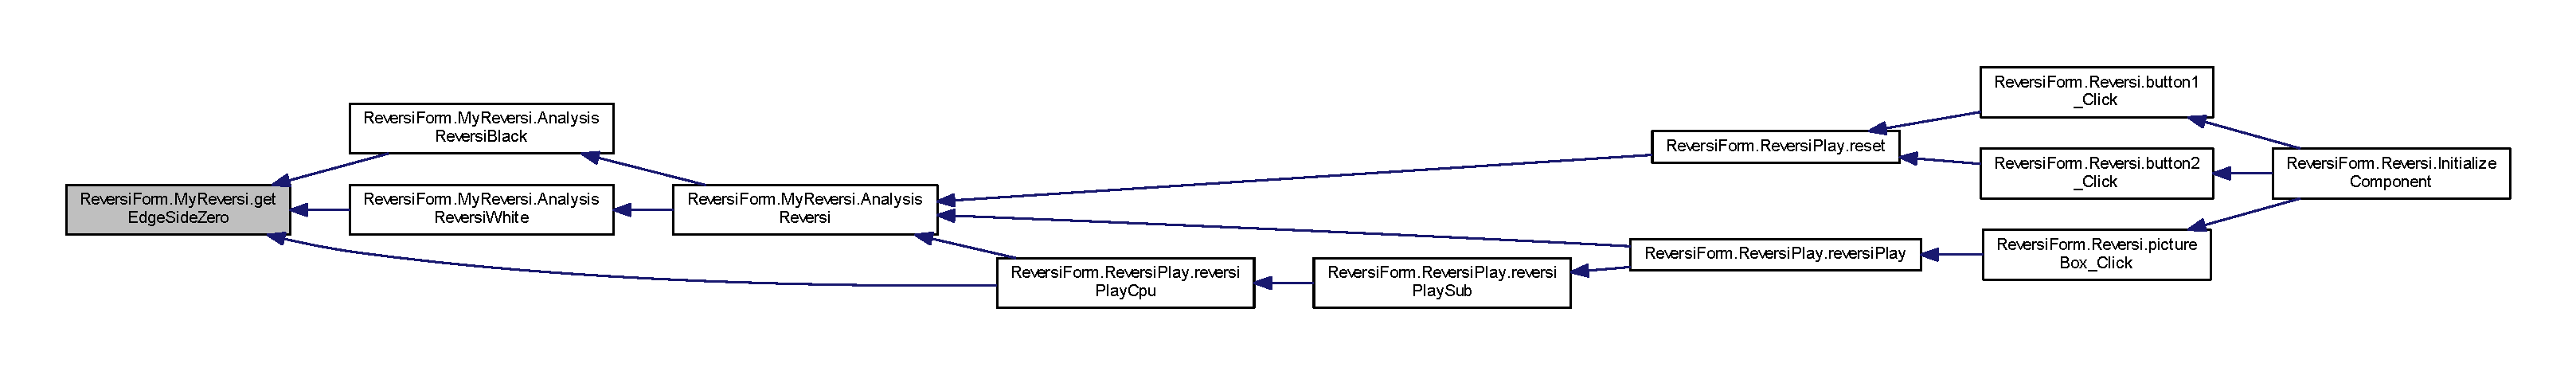
\includegraphics[width=350pt]{class_reversi_form_1_1_my_reversi_a64216270f06c7c309d39bfcb681dd1b3_icgraph}
\end{center}
\end{figure}
\mbox{\Hypertarget{class_reversi_form_1_1_my_reversi_aa39c8c111afeb4ea3bf2befbd9f1434b}\label{class_reversi_form_1_1_my_reversi_aa39c8c111afeb4ea3bf2befbd9f1434b}} 
\index{Reversi\+Form\+::\+My\+Reversi@{Reversi\+Form\+::\+My\+Reversi}!get\+Game\+End\+Sts@{get\+Game\+End\+Sts}}
\index{get\+Game\+End\+Sts@{get\+Game\+End\+Sts}!Reversi\+Form\+::\+My\+Reversi@{Reversi\+Form\+::\+My\+Reversi}}
\subsubsection{\texorpdfstring{get\+Game\+End\+Sts()}{getGameEndSts()}}
{\footnotesize\ttfamily int Reversi\+Form.\+My\+Reversi.\+get\+Game\+End\+Sts (\begin{DoxyParamCaption}{ }\end{DoxyParamCaption})}



ゲーム終了かチェック 

\begin{DoxyReturn}{Returns}
0 \+: 続行 それ以外 \+: ゲーム終了 
\end{DoxyReturn}
\begin{DoxyAuthor}{Author}
Yuta Yoshinaga 
\end{DoxyAuthor}
\begin{DoxyDate}{Date}
2017.\+10.\+20 
\end{DoxyDate}


Definition at line 1085 of file My\+Reversi.\+cs.



Referenced by Reversi\+Form.\+Reversi\+Play.\+reversi\+Play(), and Reversi\+Form.\+Reversi\+Play.\+reversi\+Play\+Sub().

Here is the call graph for this function\+:
\nopagebreak
\begin{figure}[H]
\begin{center}
\leavevmode
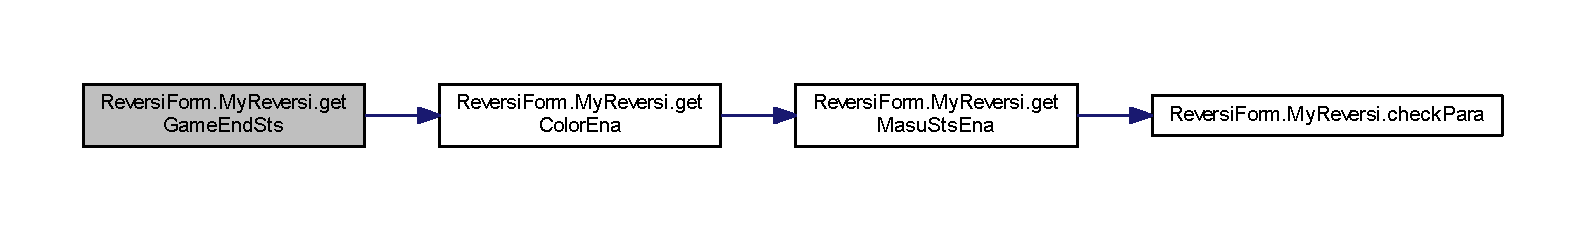
\includegraphics[width=350pt]{class_reversi_form_1_1_my_reversi_aa39c8c111afeb4ea3bf2befbd9f1434b_cgraph}
\end{center}
\end{figure}
Here is the caller graph for this function\+:
\nopagebreak
\begin{figure}[H]
\begin{center}
\leavevmode
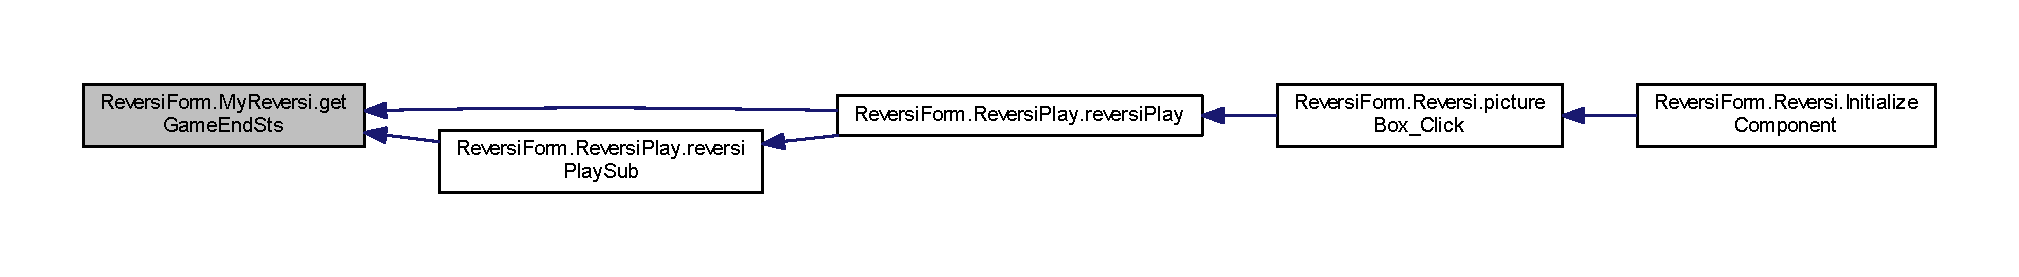
\includegraphics[width=350pt]{class_reversi_form_1_1_my_reversi_aa39c8c111afeb4ea3bf2befbd9f1434b_icgraph}
\end{center}
\end{figure}
\mbox{\Hypertarget{class_reversi_form_1_1_my_reversi_a249dba624bda1144c23cc53f68c35c67}\label{class_reversi_form_1_1_my_reversi_a249dba624bda1144c23cc53f68c35c67}} 
\index{Reversi\+Form\+::\+My\+Reversi@{Reversi\+Form\+::\+My\+Reversi}!get\+History@{get\+History}}
\index{get\+History@{get\+History}!Reversi\+Form\+::\+My\+Reversi@{Reversi\+Form\+::\+My\+Reversi}}
\subsubsection{\texorpdfstring{get\+History()}{getHistory()}}
{\footnotesize\ttfamily \hyperlink{class_reversi_form_1_1_reversi_history}{Reversi\+History} Reversi\+Form.\+My\+Reversi.\+get\+History (\begin{DoxyParamCaption}\item[{int}]{num }\end{DoxyParamCaption})}



履歴取得 


\begin{DoxyParams}[1]{Parameters}
\mbox{\tt in}  & {\em int} & num ポイント \\
\hline
\end{DoxyParams}
\begin{DoxyReturn}{Returns}
履歴 null \+: 失敗 
\end{DoxyReturn}
\begin{DoxyAuthor}{Author}
Yuta Yoshinaga 
\end{DoxyAuthor}
\begin{DoxyDate}{Date}
2017.\+10.\+20 
\end{DoxyDate}


Definition at line 1256 of file My\+Reversi.\+cs.

Here is the call graph for this function\+:
\nopagebreak
\begin{figure}[H]
\begin{center}
\leavevmode
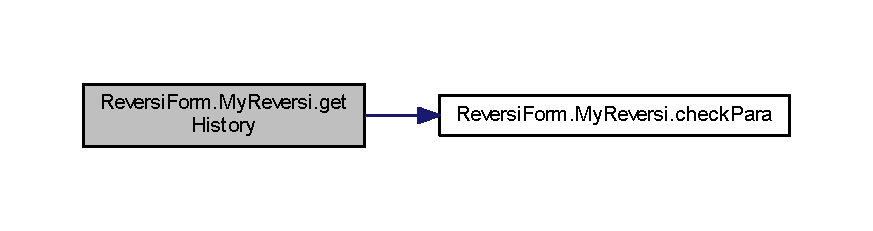
\includegraphics[width=350pt]{class_reversi_form_1_1_my_reversi_a249dba624bda1144c23cc53f68c35c67_cgraph}
\end{center}
\end{figure}
\mbox{\Hypertarget{class_reversi_form_1_1_my_reversi_a400dc82a921060bfdcf97a5fee721be1}\label{class_reversi_form_1_1_my_reversi_a400dc82a921060bfdcf97a5fee721be1}} 
\index{Reversi\+Form\+::\+My\+Reversi@{Reversi\+Form\+::\+My\+Reversi}!get\+History\+Cnt@{get\+History\+Cnt}}
\index{get\+History\+Cnt@{get\+History\+Cnt}!Reversi\+Form\+::\+My\+Reversi@{Reversi\+Form\+::\+My\+Reversi}}
\subsubsection{\texorpdfstring{get\+History\+Cnt()}{getHistoryCnt()}}
{\footnotesize\ttfamily int Reversi\+Form.\+My\+Reversi.\+get\+History\+Cnt (\begin{DoxyParamCaption}{ }\end{DoxyParamCaption})}



履歴数取得 

\begin{DoxyReturn}{Returns}
履歴数 
\end{DoxyReturn}
\begin{DoxyAuthor}{Author}
Yuta Yoshinaga 
\end{DoxyAuthor}
\begin{DoxyDate}{Date}
2017.\+10.\+20 
\end{DoxyDate}


Definition at line 1273 of file My\+Reversi.\+cs.

\mbox{\Hypertarget{class_reversi_form_1_1_my_reversi_ab6498c154199b58c418af1e0058736f6}\label{class_reversi_form_1_1_my_reversi_ab6498c154199b58c418af1e0058736f6}} 
\index{Reversi\+Form\+::\+My\+Reversi@{Reversi\+Form\+::\+My\+Reversi}!get\+Masu\+Sts@{get\+Masu\+Sts}}
\index{get\+Masu\+Sts@{get\+Masu\+Sts}!Reversi\+Form\+::\+My\+Reversi@{Reversi\+Form\+::\+My\+Reversi}}
\subsubsection{\texorpdfstring{get\+Masu\+Sts()}{getMasuSts()}}
{\footnotesize\ttfamily int Reversi\+Form.\+My\+Reversi.\+get\+Masu\+Sts (\begin{DoxyParamCaption}\item[{int}]{y,  }\item[{int}]{x }\end{DoxyParamCaption})}



マスステータスを取得 


\begin{DoxyParams}[1]{Parameters}
\mbox{\tt in}  & {\em int} & y 取得するマスの\+Y座標 \\
\hline
\mbox{\tt in}  & {\em int} & x 取得するマスの\+X座標 \\
\hline
\end{DoxyParams}
\begin{DoxyReturn}{Returns}
-\/1 \+: 失敗 それ以外 \+: マスステータス 
\end{DoxyReturn}
\begin{DoxyAuthor}{Author}
Yuta Yoshinaga 
\end{DoxyAuthor}
\begin{DoxyDate}{Date}
2017.\+10.\+20 
\end{DoxyDate}


Definition at line 988 of file My\+Reversi.\+cs.



Referenced by Reversi\+Form.\+My\+Reversi.\+check\+Edge(), Reversi\+Form.\+Reversi\+Play.\+draw\+Update(), and Reversi\+Form.\+Reversi\+Play.\+exec\+Message().

Here is the call graph for this function\+:
\nopagebreak
\begin{figure}[H]
\begin{center}
\leavevmode
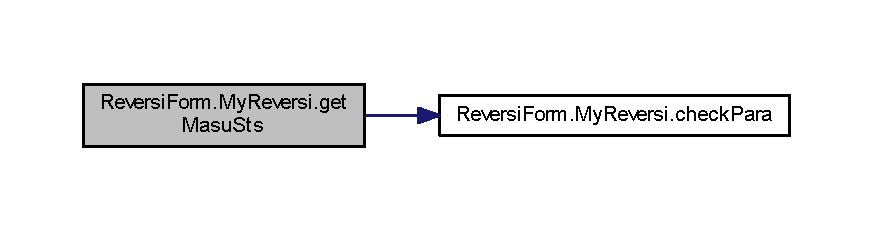
\includegraphics[width=350pt]{class_reversi_form_1_1_my_reversi_ab6498c154199b58c418af1e0058736f6_cgraph}
\end{center}
\end{figure}
Here is the caller graph for this function\+:
\nopagebreak
\begin{figure}[H]
\begin{center}
\leavevmode
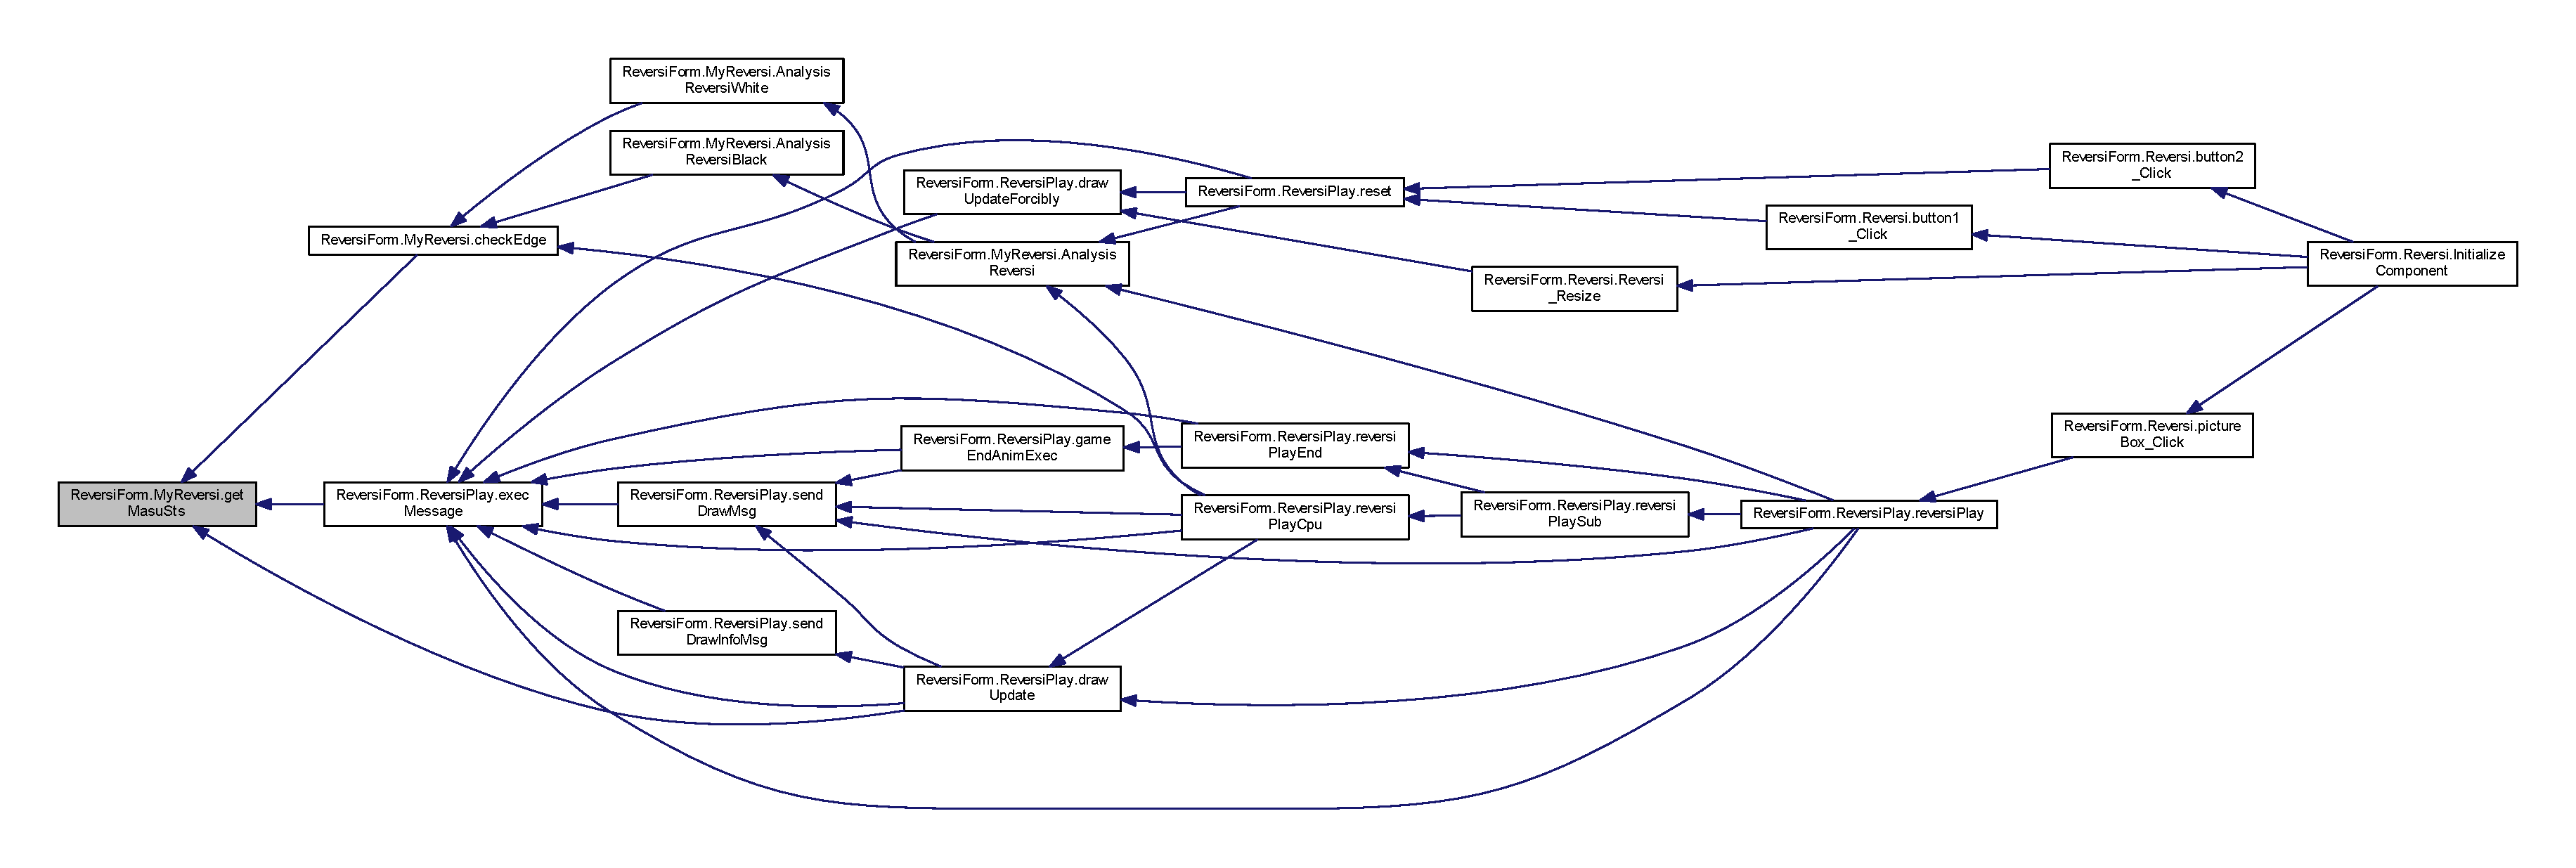
\includegraphics[width=350pt]{class_reversi_form_1_1_my_reversi_ab6498c154199b58c418af1e0058736f6_icgraph}
\end{center}
\end{figure}
\mbox{\Hypertarget{class_reversi_form_1_1_my_reversi_a26818336f7915237cf274e1fdff7ec4b}\label{class_reversi_form_1_1_my_reversi_a26818336f7915237cf274e1fdff7ec4b}} 
\index{Reversi\+Form\+::\+My\+Reversi@{Reversi\+Form\+::\+My\+Reversi}!get\+Masu\+Sts\+Cnt@{get\+Masu\+Sts\+Cnt}}
\index{get\+Masu\+Sts\+Cnt@{get\+Masu\+Sts\+Cnt}!Reversi\+Form\+::\+My\+Reversi@{Reversi\+Form\+::\+My\+Reversi}}
\subsubsection{\texorpdfstring{get\+Masu\+Sts\+Cnt()}{getMasuStsCnt()}}
{\footnotesize\ttfamily int Reversi\+Form.\+My\+Reversi.\+get\+Masu\+Sts\+Cnt (\begin{DoxyParamCaption}\item[{int}]{color,  }\item[{int}]{y,  }\item[{int}]{x }\end{DoxyParamCaption})}



指定座標の獲得コマ数取得 


\begin{DoxyParams}[1]{Parameters}
\mbox{\tt in}  & {\em int} & color コマ色 \\
\hline
\mbox{\tt in}  & {\em int} & y マスの\+Y座標 \\
\hline
\mbox{\tt in}  & {\em int} & x マスの\+X座標 \\
\hline
\end{DoxyParams}
\begin{DoxyReturn}{Returns}
-\/1 \+: 失敗 それ以外 \+: 獲得コマ数 
\end{DoxyReturn}
\begin{DoxyAuthor}{Author}
Yuta Yoshinaga 
\end{DoxyAuthor}
\begin{DoxyDate}{Date}
2017.\+10.\+20 
\end{DoxyDate}


Definition at line 1044 of file My\+Reversi.\+cs.



Referenced by Reversi\+Form.\+Reversi\+Play.\+exec\+Message(), and Reversi\+Form.\+Reversi\+Play.\+reversi\+Play\+Cpu().

Here is the call graph for this function\+:
\nopagebreak
\begin{figure}[H]
\begin{center}
\leavevmode
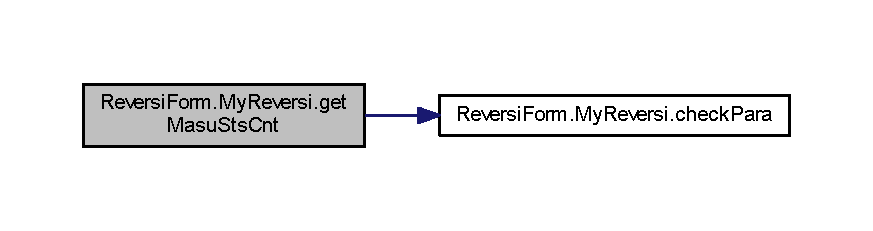
\includegraphics[width=350pt]{class_reversi_form_1_1_my_reversi_a26818336f7915237cf274e1fdff7ec4b_cgraph}
\end{center}
\end{figure}
Here is the caller graph for this function\+:
\nopagebreak
\begin{figure}[H]
\begin{center}
\leavevmode
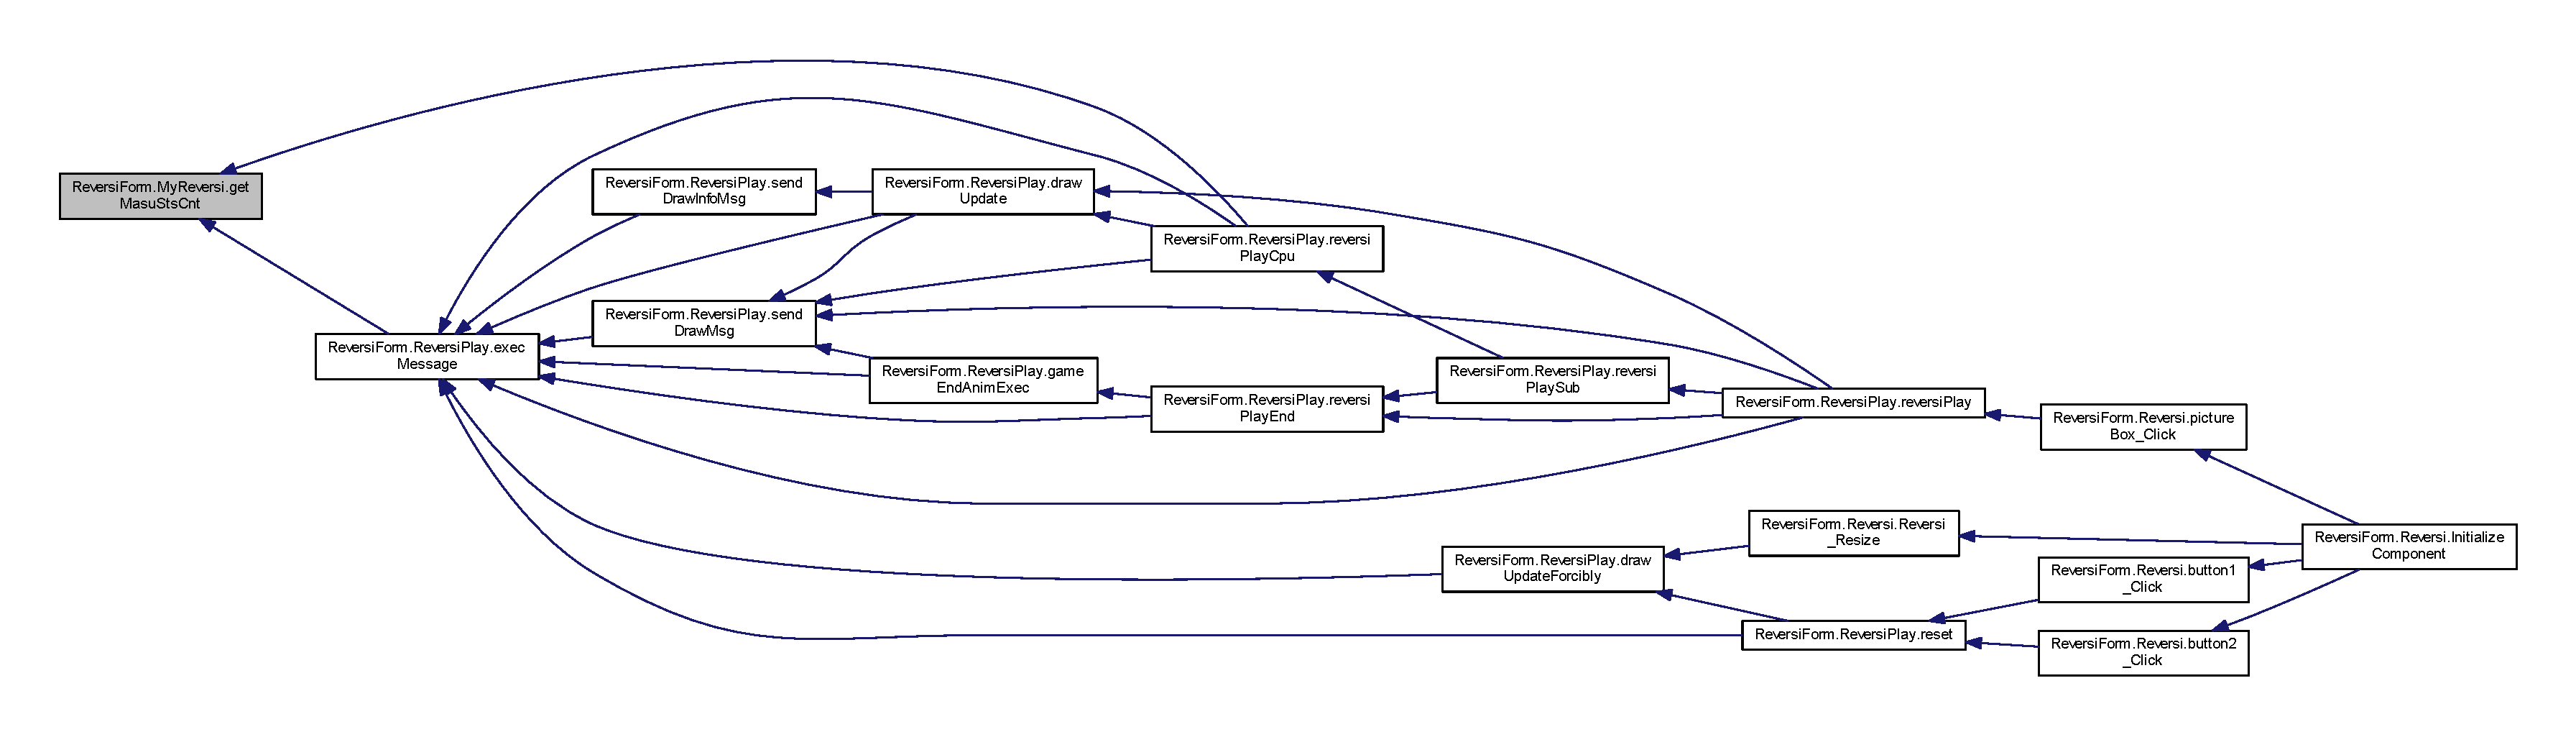
\includegraphics[width=350pt]{class_reversi_form_1_1_my_reversi_a26818336f7915237cf274e1fdff7ec4b_icgraph}
\end{center}
\end{figure}
\mbox{\Hypertarget{class_reversi_form_1_1_my_reversi_ae8404068c47751d53c4b430d635a1bb2}\label{class_reversi_form_1_1_my_reversi_ae8404068c47751d53c4b430d635a1bb2}} 
\index{Reversi\+Form\+::\+My\+Reversi@{Reversi\+Form\+::\+My\+Reversi}!get\+Masu\+Sts\+Ena@{get\+Masu\+Sts\+Ena}}
\index{get\+Masu\+Sts\+Ena@{get\+Masu\+Sts\+Ena}!Reversi\+Form\+::\+My\+Reversi@{Reversi\+Form\+::\+My\+Reversi}}
\subsubsection{\texorpdfstring{get\+Masu\+Sts\+Ena()}{getMasuStsEna()}}
{\footnotesize\ttfamily int Reversi\+Form.\+My\+Reversi.\+get\+Masu\+Sts\+Ena (\begin{DoxyParamCaption}\item[{int}]{color,  }\item[{int}]{y,  }\item[{int}]{x }\end{DoxyParamCaption})}



指定座標に指定色を置けるかチェック 


\begin{DoxyParams}[1]{Parameters}
\mbox{\tt in}  & {\em int} & color コマ色 \\
\hline
\mbox{\tt in}  & {\em int} & y マスの\+Y座標 \\
\hline
\mbox{\tt in}  & {\em int} & x マスの\+X座標 \\
\hline
\end{DoxyParams}
\begin{DoxyReturn}{Returns}
1 \+: 成功 それ以外 \+: 失敗 
\end{DoxyReturn}
\begin{DoxyAuthor}{Author}
Yuta Yoshinaga 
\end{DoxyAuthor}
\begin{DoxyDate}{Date}
2017.\+10.\+20 
\end{DoxyDate}


Definition at line 1023 of file My\+Reversi.\+cs.



Referenced by Reversi\+Form.\+My\+Reversi.\+Analysis\+Reversi\+Black(), Reversi\+Form.\+My\+Reversi.\+Analysis\+Reversi\+White(), Reversi\+Form.\+Reversi\+Play.\+exec\+Message(), Reversi\+Form.\+My\+Reversi.\+get\+Color\+Ena(), Reversi\+Form.\+Reversi\+Play.\+reversi\+Play\+Cpu(), and Reversi\+Form.\+My\+Reversi.\+set\+Masu\+Sts().

Here is the call graph for this function\+:
\nopagebreak
\begin{figure}[H]
\begin{center}
\leavevmode
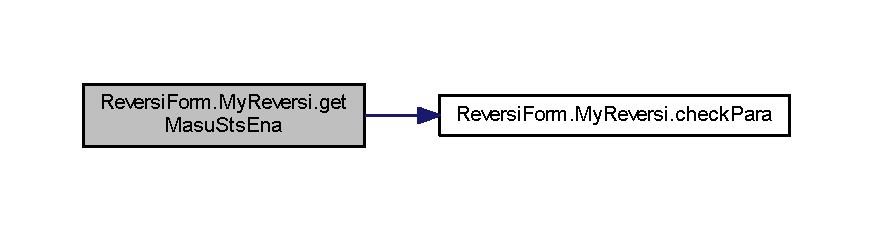
\includegraphics[width=350pt]{class_reversi_form_1_1_my_reversi_ae8404068c47751d53c4b430d635a1bb2_cgraph}
\end{center}
\end{figure}
Here is the caller graph for this function\+:
\nopagebreak
\begin{figure}[H]
\begin{center}
\leavevmode
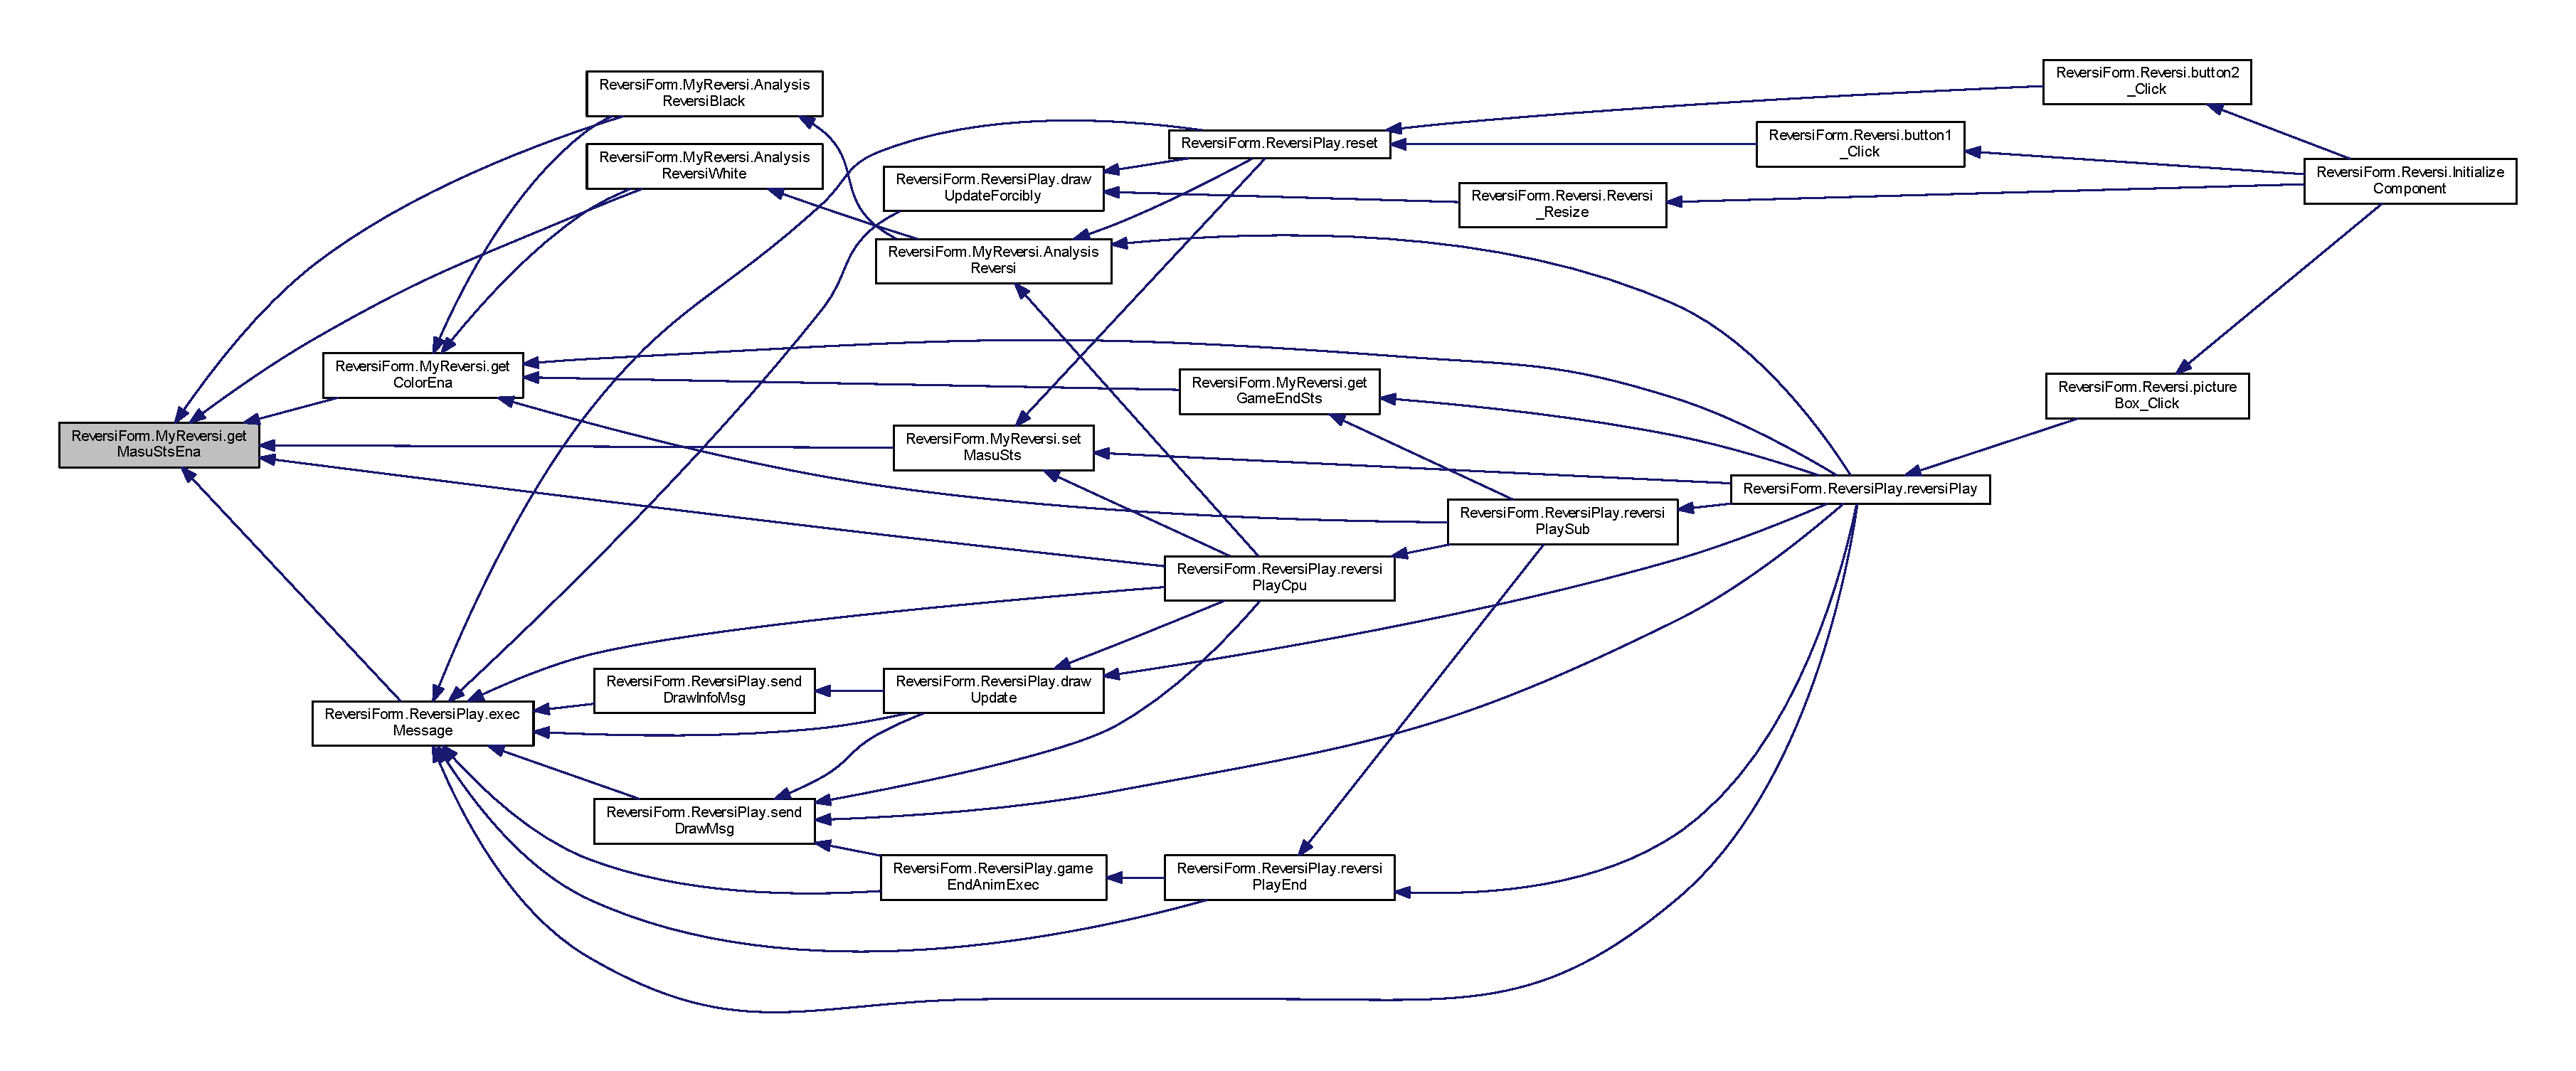
\includegraphics[width=350pt]{class_reversi_form_1_1_my_reversi_ae8404068c47751d53c4b430d635a1bb2_icgraph}
\end{center}
\end{figure}
\mbox{\Hypertarget{class_reversi_form_1_1_my_reversi_abd6f4b9d6355af3175ac885731338705}\label{class_reversi_form_1_1_my_reversi_abd6f4b9d6355af3175ac885731338705}} 
\index{Reversi\+Form\+::\+My\+Reversi@{Reversi\+Form\+::\+My\+Reversi}!get\+Masu\+Sts\+Old@{get\+Masu\+Sts\+Old}}
\index{get\+Masu\+Sts\+Old@{get\+Masu\+Sts\+Old}!Reversi\+Form\+::\+My\+Reversi@{Reversi\+Form\+::\+My\+Reversi}}
\subsubsection{\texorpdfstring{get\+Masu\+Sts\+Old()}{getMasuStsOld()}}
{\footnotesize\ttfamily int Reversi\+Form.\+My\+Reversi.\+get\+Masu\+Sts\+Old (\begin{DoxyParamCaption}\item[{int}]{y,  }\item[{int}]{x }\end{DoxyParamCaption})}



以前のマスステータスを取得 


\begin{DoxyParams}[1]{Parameters}
\mbox{\tt in}  & {\em int} & y 取得するマスの\+Y座標 \\
\hline
\mbox{\tt in}  & {\em int} & x 取得するマスの\+X座標 \\
\hline
\end{DoxyParams}
\begin{DoxyReturn}{Returns}
-\/1 \+: 失敗 それ以外 \+: マスステータス 
\end{DoxyReturn}
\begin{DoxyAuthor}{Author}
Yuta Yoshinaga 
\end{DoxyAuthor}
\begin{DoxyDate}{Date}
2017.\+10.\+20 
\end{DoxyDate}


Definition at line 1005 of file My\+Reversi.\+cs.



Referenced by Reversi\+Form.\+Reversi\+Play.\+draw\+Update().

Here is the call graph for this function\+:
\nopagebreak
\begin{figure}[H]
\begin{center}
\leavevmode
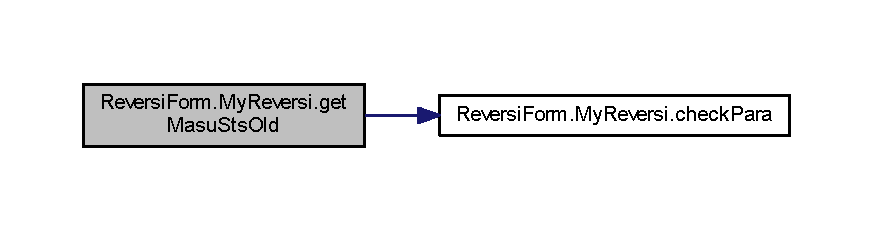
\includegraphics[width=350pt]{class_reversi_form_1_1_my_reversi_abd6f4b9d6355af3175ac885731338705_cgraph}
\end{center}
\end{figure}
Here is the caller graph for this function\+:
\nopagebreak
\begin{figure}[H]
\begin{center}
\leavevmode
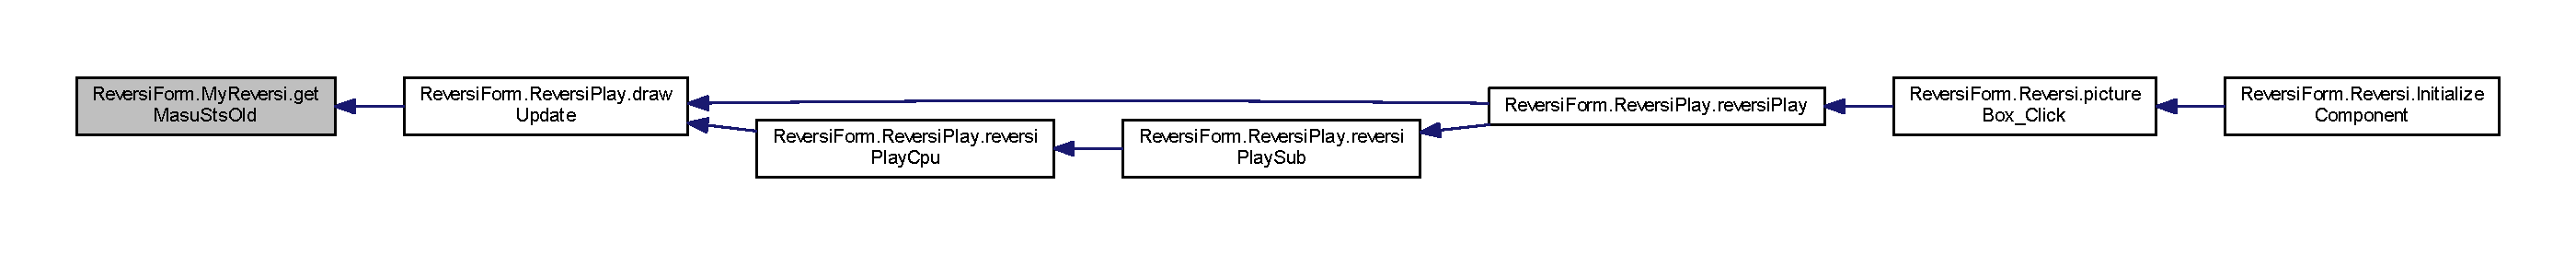
\includegraphics[width=350pt]{class_reversi_form_1_1_my_reversi_abd6f4b9d6355af3175ac885731338705_icgraph}
\end{center}
\end{figure}
\mbox{\Hypertarget{class_reversi_form_1_1_my_reversi_a13c780ba2b5a346bd6fd295a0cc962f8}\label{class_reversi_form_1_1_my_reversi_a13c780ba2b5a346bd6fd295a0cc962f8}} 
\index{Reversi\+Form\+::\+My\+Reversi@{Reversi\+Form\+::\+My\+Reversi}!get\+Pass\+Ena@{get\+Pass\+Ena}}
\index{get\+Pass\+Ena@{get\+Pass\+Ena}!Reversi\+Form\+::\+My\+Reversi@{Reversi\+Form\+::\+My\+Reversi}}
\subsubsection{\texorpdfstring{get\+Pass\+Ena()}{getPassEna()}}
{\footnotesize\ttfamily int Reversi\+Form.\+My\+Reversi.\+get\+Pass\+Ena (\begin{DoxyParamCaption}\item[{int}]{color,  }\item[{int}]{y,  }\item[{int}]{x }\end{DoxyParamCaption})}



パス判定 


\begin{DoxyParams}[1]{Parameters}
\mbox{\tt in}  & {\em int} & color コマ色 \\
\hline
\mbox{\tt in}  & {\em int} & y マスの\+Y座標 \\
\hline
\mbox{\tt in}  & {\em int} & x マスの\+X座標 \\
\hline
\end{DoxyParams}
\begin{DoxyReturn}{Returns}
パス判定
\begin{DoxyItemize}
\item 0 \+: N\+OT P\+A\+SS
\item 1 \+: P\+A\+SS
\end{DoxyItemize}
\end{DoxyReturn}
\begin{DoxyAuthor}{Author}
Yuta Yoshinaga 
\end{DoxyAuthor}
\begin{DoxyDate}{Date}
2017.\+10.\+20 
\end{DoxyDate}


Definition at line 1237 of file My\+Reversi.\+cs.



Referenced by Reversi\+Form.\+Reversi\+Play.\+reversi\+Play\+Cpu().

Here is the call graph for this function\+:
\nopagebreak
\begin{figure}[H]
\begin{center}
\leavevmode
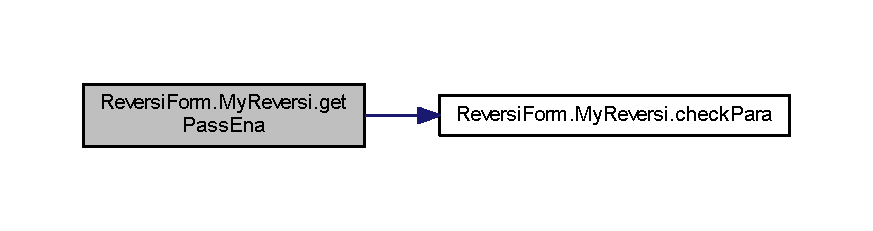
\includegraphics[width=350pt]{class_reversi_form_1_1_my_reversi_a13c780ba2b5a346bd6fd295a0cc962f8_cgraph}
\end{center}
\end{figure}
Here is the caller graph for this function\+:
\nopagebreak
\begin{figure}[H]
\begin{center}
\leavevmode
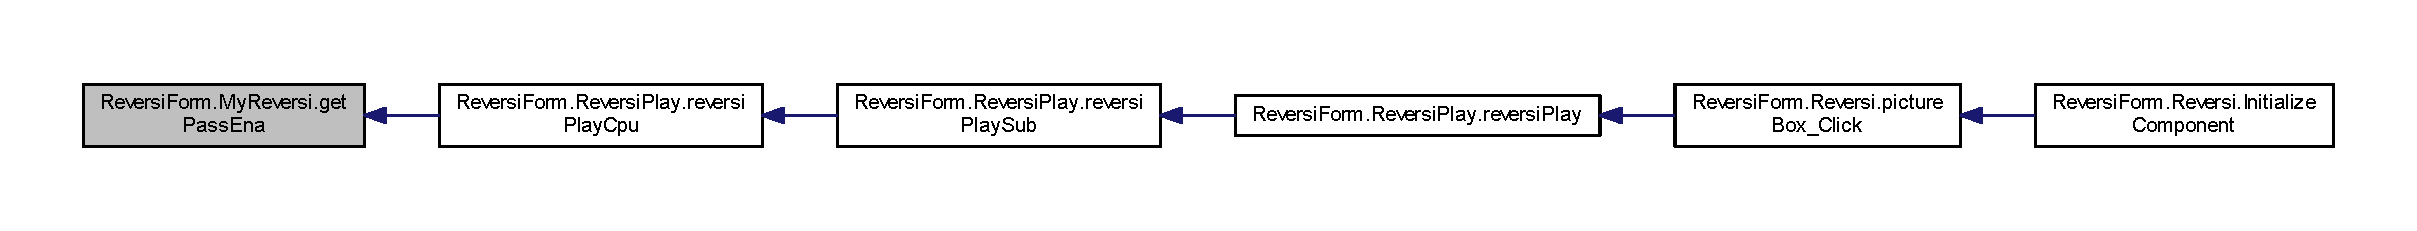
\includegraphics[width=350pt]{class_reversi_form_1_1_my_reversi_a13c780ba2b5a346bd6fd295a0cc962f8_icgraph}
\end{center}
\end{figure}
\mbox{\Hypertarget{class_reversi_form_1_1_my_reversi_a58150a220368d7d7ae8ad01ee0120e71}\label{class_reversi_form_1_1_my_reversi_a58150a220368d7d7ae8ad01ee0120e71}} 
\index{Reversi\+Form\+::\+My\+Reversi@{Reversi\+Form\+::\+My\+Reversi}!get\+Point@{get\+Point}}
\index{get\+Point@{get\+Point}!Reversi\+Form\+::\+My\+Reversi@{Reversi\+Form\+::\+My\+Reversi}}
\subsubsection{\texorpdfstring{get\+Point()}{getPoint()}}
{\footnotesize\ttfamily \hyperlink{class_reversi_form_1_1_reversi_point}{Reversi\+Point} Reversi\+Form.\+My\+Reversi.\+get\+Point (\begin{DoxyParamCaption}\item[{int}]{color,  }\item[{int}]{num }\end{DoxyParamCaption})}



ポイント座標取得 


\begin{DoxyParams}[1]{Parameters}
\mbox{\tt in}  & {\em int} & color コマ色 \\
\hline
\mbox{\tt in}  & {\em int} & num ポイント \\
\hline
\end{DoxyParams}
\begin{DoxyReturn}{Returns}
ポイント座標 null \+: 失敗 
\end{DoxyReturn}
\begin{DoxyAuthor}{Author}
Yuta Yoshinaga 
\end{DoxyAuthor}
\begin{DoxyDate}{Date}
2017.\+10.\+20 
\end{DoxyDate}


Definition at line 1179 of file My\+Reversi.\+cs.



Referenced by Reversi\+Form.\+Reversi\+Play.\+reset(), and Reversi\+Form.\+Reversi\+Play.\+reversi\+Play\+Cpu().

Here is the call graph for this function\+:
\nopagebreak
\begin{figure}[H]
\begin{center}
\leavevmode
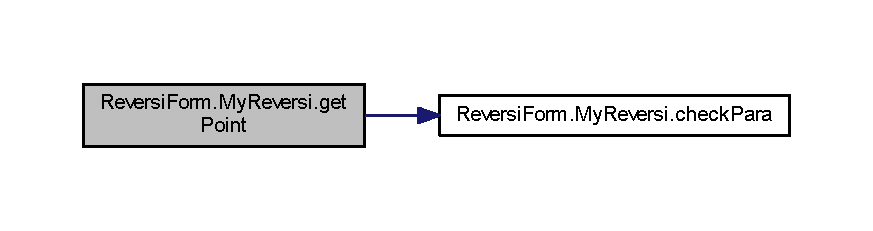
\includegraphics[width=350pt]{class_reversi_form_1_1_my_reversi_a58150a220368d7d7ae8ad01ee0120e71_cgraph}
\end{center}
\end{figure}
Here is the caller graph for this function\+:
\nopagebreak
\begin{figure}[H]
\begin{center}
\leavevmode
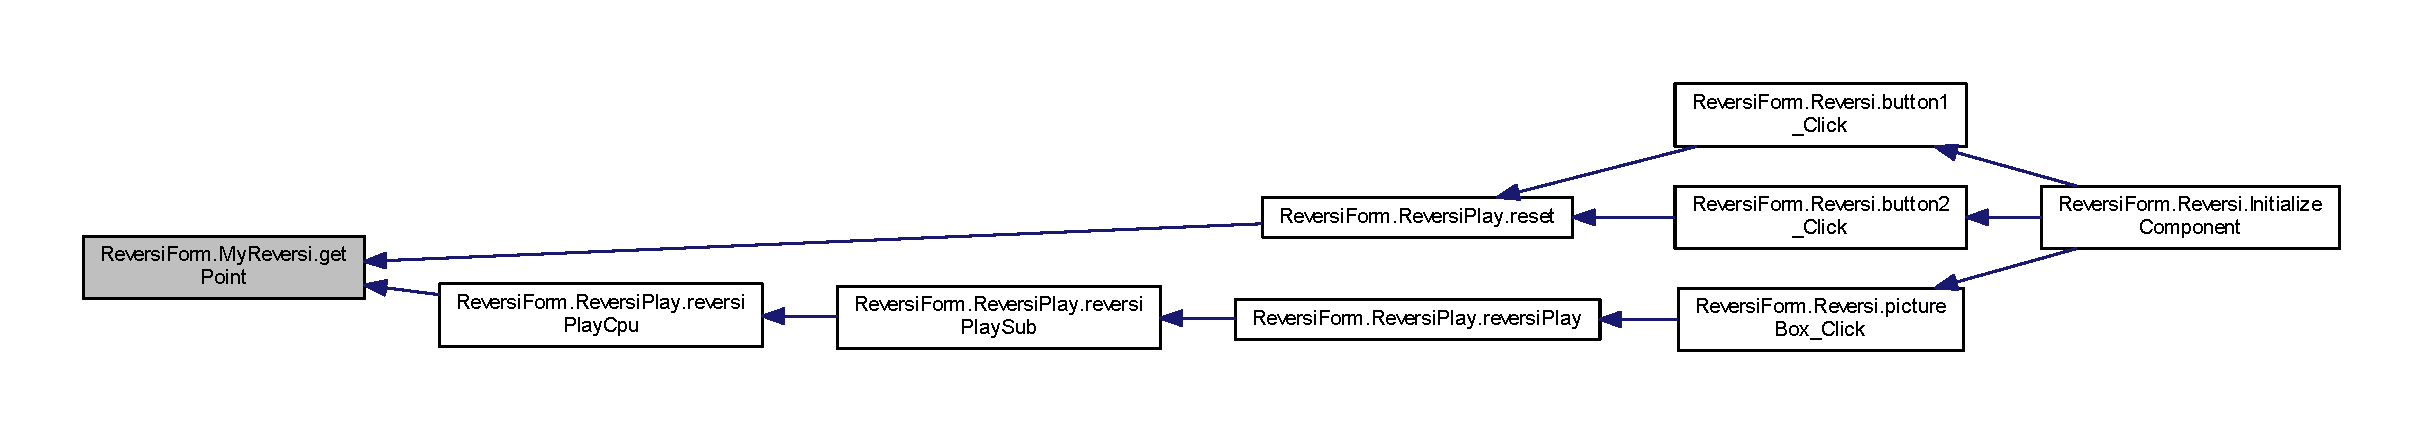
\includegraphics[width=350pt]{class_reversi_form_1_1_my_reversi_a58150a220368d7d7ae8ad01ee0120e71_icgraph}
\end{center}
\end{figure}
\mbox{\Hypertarget{class_reversi_form_1_1_my_reversi_af0170bf211a996c2285d0db926f2f0ae}\label{class_reversi_form_1_1_my_reversi_af0170bf211a996c2285d0db926f2f0ae}} 
\index{Reversi\+Form\+::\+My\+Reversi@{Reversi\+Form\+::\+My\+Reversi}!get\+Point\+Anz@{get\+Point\+Anz}}
\index{get\+Point\+Anz@{get\+Point\+Anz}!Reversi\+Form\+::\+My\+Reversi@{Reversi\+Form\+::\+My\+Reversi}}
\subsubsection{\texorpdfstring{get\+Point\+Anz()}{getPointAnz()}}
{\footnotesize\ttfamily \hyperlink{class_reversi_form_1_1_reversi_anz}{Reversi\+Anz} Reversi\+Form.\+My\+Reversi.\+get\+Point\+Anz (\begin{DoxyParamCaption}\item[{int}]{color,  }\item[{int}]{y,  }\item[{int}]{x }\end{DoxyParamCaption})}



ポイント座標解析取得 


\begin{DoxyParams}[1]{Parameters}
\mbox{\tt in}  & {\em int} & color コマ色 \\
\hline
\mbox{\tt in}  & {\em int} & y マスの\+Y座標 \\
\hline
\mbox{\tt in}  & {\em int} & x マスの\+X座標 \\
\hline
\end{DoxyParams}
\begin{DoxyReturn}{Returns}
ポイント座標解析 null \+: 失敗 
\end{DoxyReturn}
\begin{DoxyAuthor}{Author}
Yuta Yoshinaga 
\end{DoxyAuthor}
\begin{DoxyDate}{Date}
2017.\+10.\+20 
\end{DoxyDate}


Definition at line 1291 of file My\+Reversi.\+cs.



Referenced by Reversi\+Form.\+Reversi\+Play.\+reversi\+Play\+Cpu().

Here is the call graph for this function\+:
\nopagebreak
\begin{figure}[H]
\begin{center}
\leavevmode
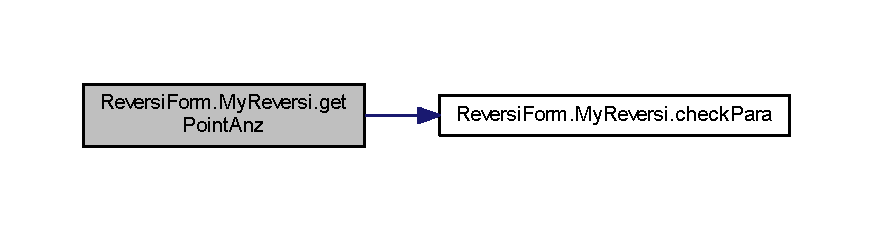
\includegraphics[width=350pt]{class_reversi_form_1_1_my_reversi_af0170bf211a996c2285d0db926f2f0ae_cgraph}
\end{center}
\end{figure}
Here is the caller graph for this function\+:
\nopagebreak
\begin{figure}[H]
\begin{center}
\leavevmode
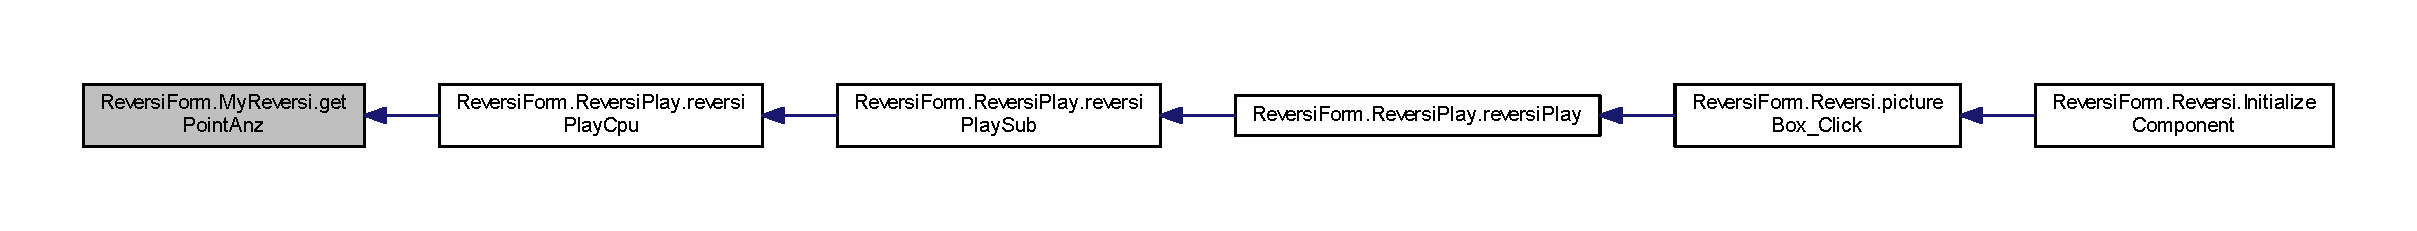
\includegraphics[width=350pt]{class_reversi_form_1_1_my_reversi_af0170bf211a996c2285d0db926f2f0ae_icgraph}
\end{center}
\end{figure}
\mbox{\Hypertarget{class_reversi_form_1_1_my_reversi_a7b5ebbdd9b7ff56d72185e6b89a50af8}\label{class_reversi_form_1_1_my_reversi_a7b5ebbdd9b7ff56d72185e6b89a50af8}} 
\index{Reversi\+Form\+::\+My\+Reversi@{Reversi\+Form\+::\+My\+Reversi}!get\+Point\+Cnt@{get\+Point\+Cnt}}
\index{get\+Point\+Cnt@{get\+Point\+Cnt}!Reversi\+Form\+::\+My\+Reversi@{Reversi\+Form\+::\+My\+Reversi}}
\subsubsection{\texorpdfstring{get\+Point\+Cnt()}{getPointCnt()}}
{\footnotesize\ttfamily int Reversi\+Form.\+My\+Reversi.\+get\+Point\+Cnt (\begin{DoxyParamCaption}\item[{int}]{color }\end{DoxyParamCaption})}



ポイント座標数取得 


\begin{DoxyParams}[1]{Parameters}
\mbox{\tt in}  & {\em int} & color コマ色 \\
\hline
\end{DoxyParams}
\begin{DoxyReturn}{Returns}
ポイント座標数取得 
\end{DoxyReturn}
\begin{DoxyAuthor}{Author}
Yuta Yoshinaga 
\end{DoxyAuthor}
\begin{DoxyDate}{Date}
2017.\+10.\+20 
\end{DoxyDate}


Definition at line 1198 of file My\+Reversi.\+cs.



Referenced by Reversi\+Form.\+My\+Reversi.\+Analysis\+Reversi\+Black(), Reversi\+Form.\+My\+Reversi.\+Analysis\+Reversi\+White(), Reversi\+Form.\+Reversi\+Play.\+reset(), and Reversi\+Form.\+Reversi\+Play.\+reversi\+Play\+Cpu().

Here is the caller graph for this function\+:
\nopagebreak
\begin{figure}[H]
\begin{center}
\leavevmode
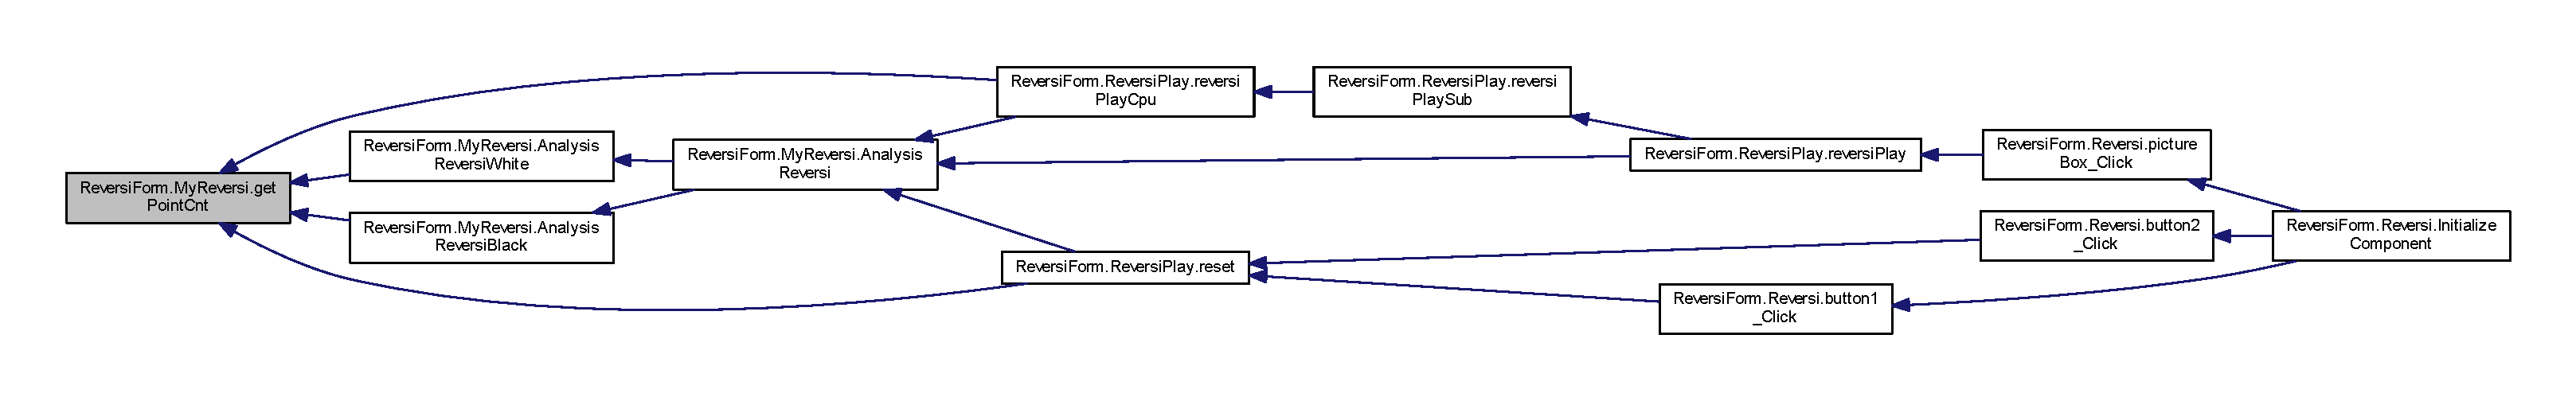
\includegraphics[width=350pt]{class_reversi_form_1_1_my_reversi_a7b5ebbdd9b7ff56d72185e6b89a50af8_icgraph}
\end{center}
\end{figure}
\mbox{\Hypertarget{class_reversi_form_1_1_my_reversi_a379ac04ab0e8e9fc819ef3ceeba63e58}\label{class_reversi_form_1_1_my_reversi_a379ac04ab0e8e9fc819ef3ceeba63e58}} 
\index{Reversi\+Form\+::\+My\+Reversi@{Reversi\+Form\+::\+My\+Reversi}!make\+Masu\+Sts@{make\+Masu\+Sts}}
\index{make\+Masu\+Sts@{make\+Masu\+Sts}!Reversi\+Form\+::\+My\+Reversi@{Reversi\+Form\+::\+My\+Reversi}}
\subsubsection{\texorpdfstring{make\+Masu\+Sts()}{makeMasuSts()}}
{\footnotesize\ttfamily int Reversi\+Form.\+My\+Reversi.\+make\+Masu\+Sts (\begin{DoxyParamCaption}\item[{int}]{color }\end{DoxyParamCaption})\hspace{0.3cm}{\ttfamily [private]}}



各コマの置ける場所等のステータス作成 


\begin{DoxyParams}[1]{Parameters}
\mbox{\tt in}  & {\em int} & color ステータスを作成するコマ \\
\hline
\end{DoxyParams}
\begin{DoxyReturn}{Returns}
ありません 
\end{DoxyReturn}
\begin{DoxyAuthor}{Author}
Yuta Yoshinaga 
\end{DoxyAuthor}
\begin{DoxyDate}{Date}
2017.\+10.\+20 
\end{DoxyDate}


Definition at line 273 of file My\+Reversi.\+cs.



Referenced by Reversi\+Form.\+My\+Reversi.\+Analysis\+Reversi(), Reversi\+Form.\+My\+Reversi.\+Analysis\+Reversi\+Black(), Reversi\+Form.\+My\+Reversi.\+Analysis\+Reversi\+White(), Reversi\+Form.\+My\+Reversi.\+reset(), and Reversi\+Form.\+My\+Reversi.\+set\+Masu\+Sts().

Here is the caller graph for this function\+:
\nopagebreak
\begin{figure}[H]
\begin{center}
\leavevmode
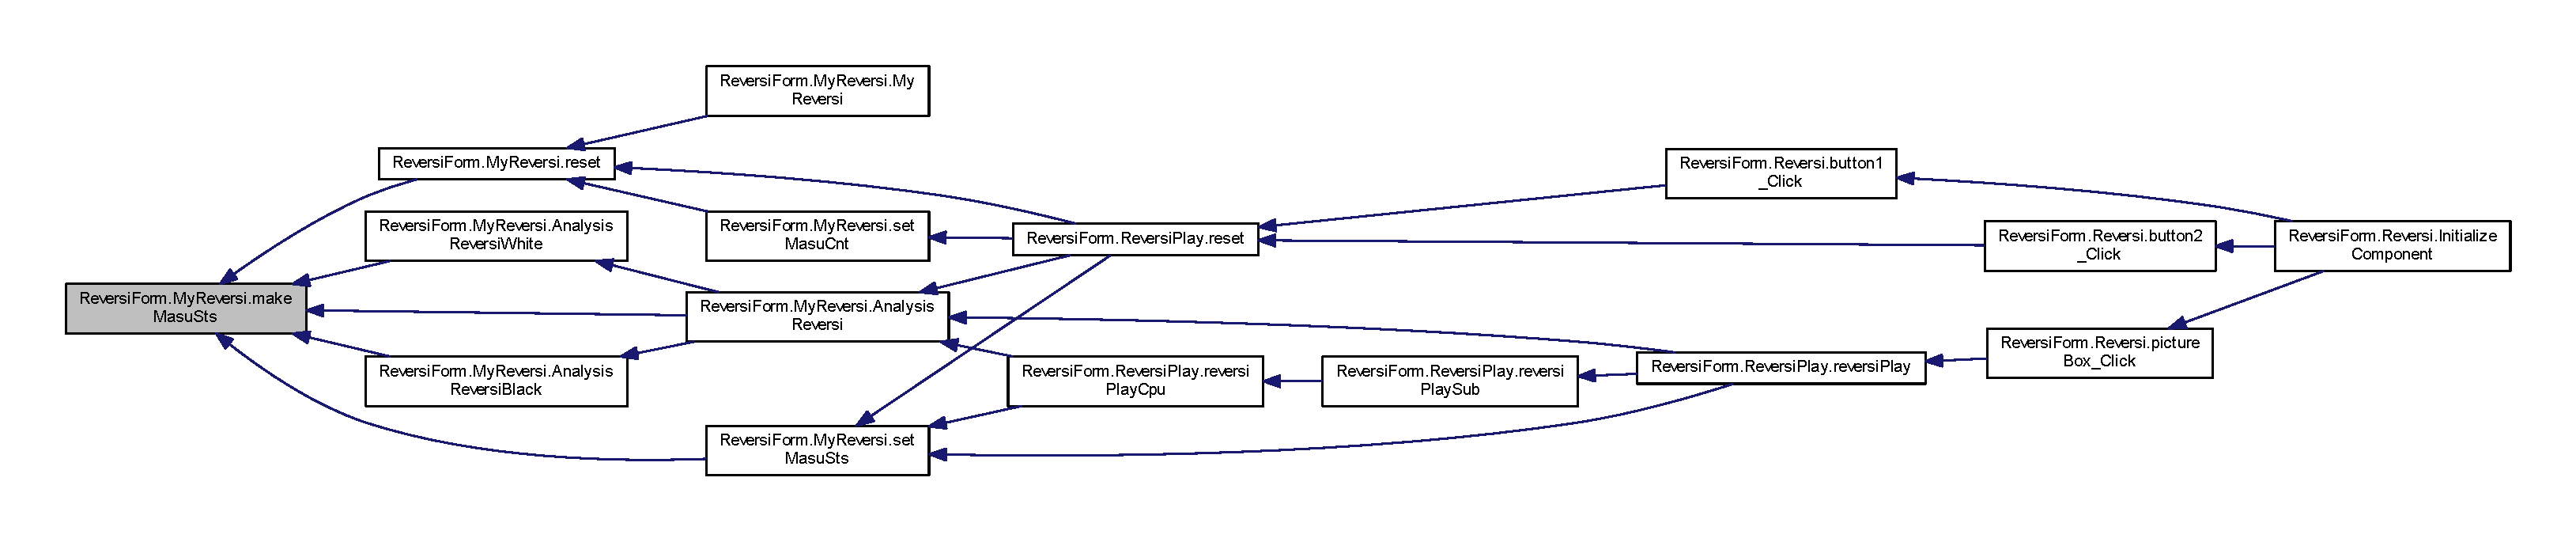
\includegraphics[width=350pt]{class_reversi_form_1_1_my_reversi_a379ac04ab0e8e9fc819ef3ceeba63e58_icgraph}
\end{center}
\end{figure}
\mbox{\Hypertarget{class_reversi_form_1_1_my_reversi_aa8d8e839466c63462954080353cd4a9e}\label{class_reversi_form_1_1_my_reversi_aa8d8e839466c63462954080353cd4a9e}} 
\index{Reversi\+Form\+::\+My\+Reversi@{Reversi\+Form\+::\+My\+Reversi}!reset@{reset}}
\index{reset@{reset}!Reversi\+Form\+::\+My\+Reversi@{Reversi\+Form\+::\+My\+Reversi}}
\subsubsection{\texorpdfstring{reset()}{reset()}}
{\footnotesize\ttfamily void Reversi\+Form.\+My\+Reversi.\+reset (\begin{DoxyParamCaption}{ }\end{DoxyParamCaption})}



リセット 

\begin{DoxyReturn}{Returns}
ありません 
\end{DoxyReturn}
\begin{DoxyAuthor}{Author}
Yuta Yoshinaga 
\end{DoxyAuthor}
\begin{DoxyDate}{Date}
2017.\+10.\+20 
\end{DoxyDate}


Definition at line 243 of file My\+Reversi.\+cs.



Referenced by Reversi\+Form.\+My\+Reversi.\+My\+Reversi(), Reversi\+Form.\+Reversi\+Play.\+reset(), and Reversi\+Form.\+My\+Reversi.\+set\+Masu\+Cnt().

Here is the call graph for this function\+:
\nopagebreak
\begin{figure}[H]
\begin{center}
\leavevmode
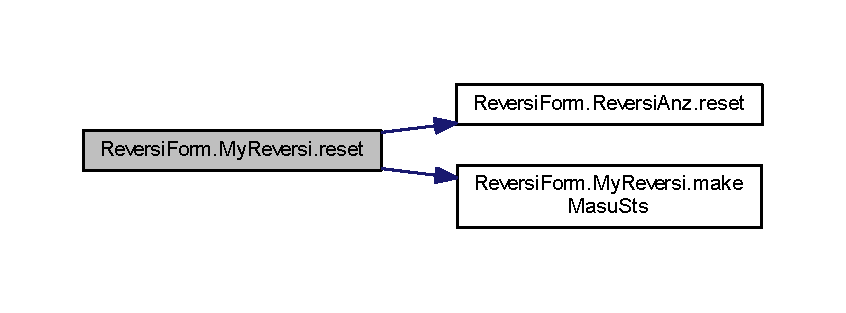
\includegraphics[width=350pt]{class_reversi_form_1_1_my_reversi_aa8d8e839466c63462954080353cd4a9e_cgraph}
\end{center}
\end{figure}
Here is the caller graph for this function\+:
\nopagebreak
\begin{figure}[H]
\begin{center}
\leavevmode
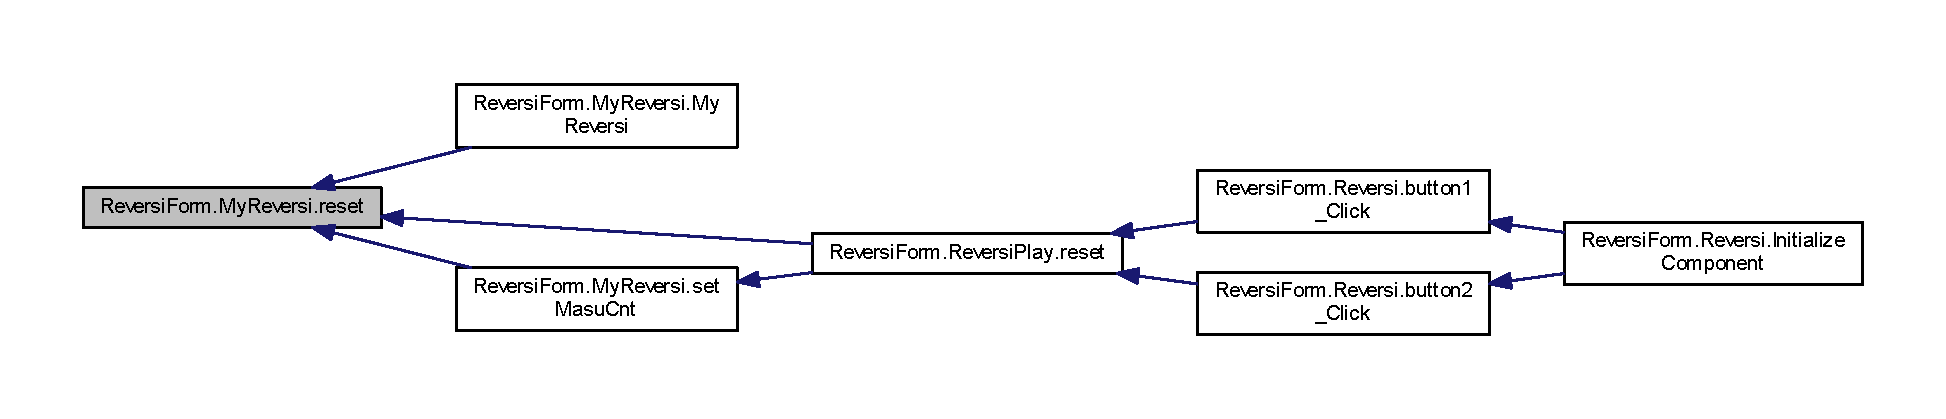
\includegraphics[width=350pt]{class_reversi_form_1_1_my_reversi_aa8d8e839466c63462954080353cd4a9e_icgraph}
\end{center}
\end{figure}
\mbox{\Hypertarget{class_reversi_form_1_1_my_reversi_a990acf71124e50643c0774c38f8f634b}\label{class_reversi_form_1_1_my_reversi_a990acf71124e50643c0774c38f8f634b}} 
\index{Reversi\+Form\+::\+My\+Reversi@{Reversi\+Form\+::\+My\+Reversi}!rev\+Masu\+Sts@{rev\+Masu\+Sts}}
\index{rev\+Masu\+Sts@{rev\+Masu\+Sts}!Reversi\+Form\+::\+My\+Reversi@{Reversi\+Form\+::\+My\+Reversi}}
\subsubsection{\texorpdfstring{rev\+Masu\+Sts()}{revMasuSts()}}
{\footnotesize\ttfamily void Reversi\+Form.\+My\+Reversi.\+rev\+Masu\+Sts (\begin{DoxyParamCaption}\item[{int}]{color,  }\item[{int}]{y,  }\item[{int}]{x }\end{DoxyParamCaption})\hspace{0.3cm}{\ttfamily [private]}}



コマをひっくり返す 


\begin{DoxyParams}[1]{Parameters}
\mbox{\tt in}  & {\em int} & color ひっくり返す元コマ \\
\hline
\mbox{\tt in}  & {\em int} & y ひっくり返す元コマの\+Y座標 \\
\hline
\mbox{\tt in}  & {\em int} & x ひっくり返す元コマの\+X座標 \\
\hline
\end{DoxyParams}
\begin{DoxyReturn}{Returns}
ありません 
\end{DoxyReturn}
\begin{DoxyAuthor}{Author}
Yuta Yoshinaga 
\end{DoxyAuthor}
\begin{DoxyDate}{Date}
2017.\+10.\+20 
\end{DoxyDate}


Definition at line 479 of file My\+Reversi.\+cs.



Referenced by Reversi\+Form.\+My\+Reversi.\+Analysis\+Reversi\+Black(), Reversi\+Form.\+My\+Reversi.\+Analysis\+Reversi\+White(), and Reversi\+Form.\+My\+Reversi.\+set\+Masu\+Sts().

Here is the caller graph for this function\+:
\nopagebreak
\begin{figure}[H]
\begin{center}
\leavevmode
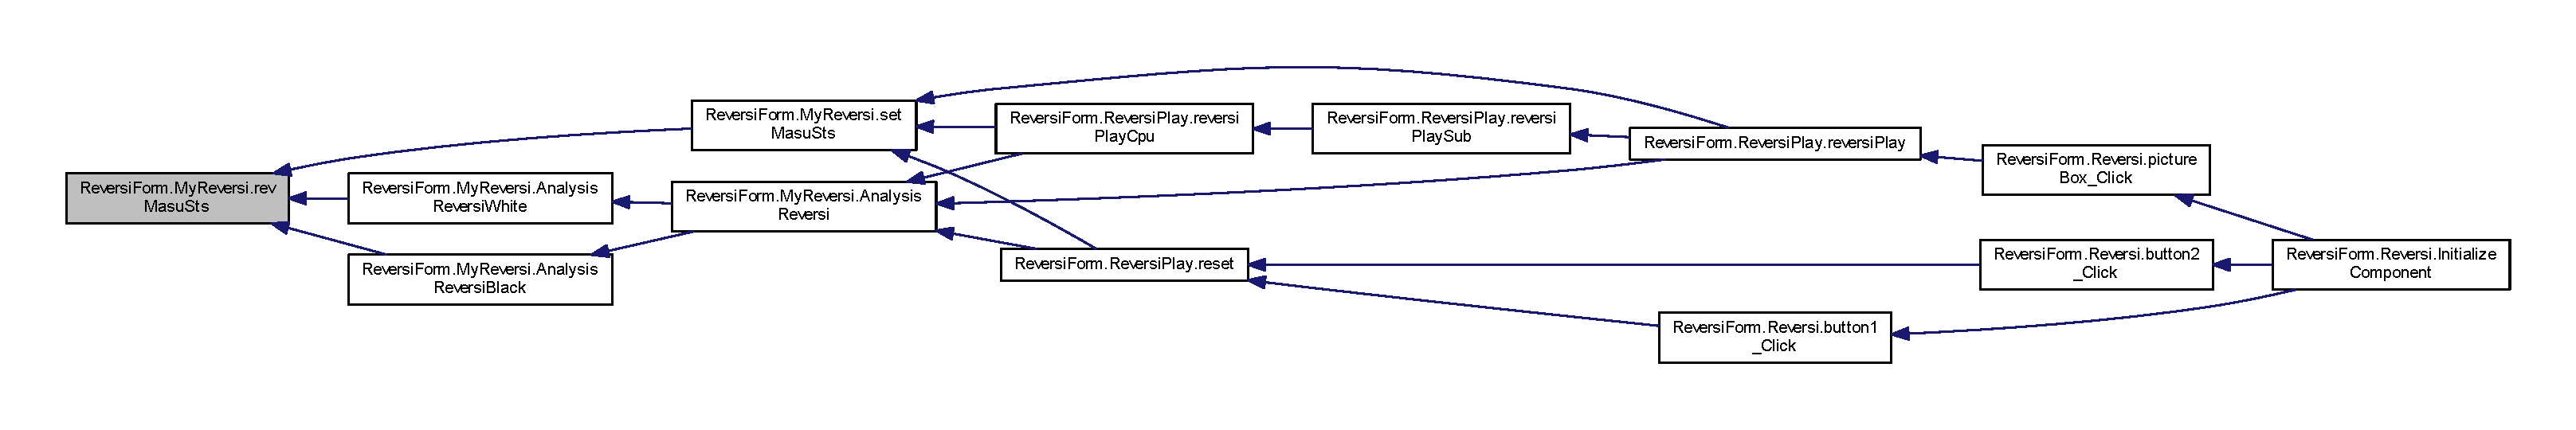
\includegraphics[width=350pt]{class_reversi_form_1_1_my_reversi_a990acf71124e50643c0774c38f8f634b_icgraph}
\end{center}
\end{figure}
\mbox{\Hypertarget{class_reversi_form_1_1_my_reversi_af9573f1da0d89180a4dbbd98d41a05fb}\label{class_reversi_form_1_1_my_reversi_af9573f1da0d89180a4dbbd98d41a05fb}} 
\index{Reversi\+Form\+::\+My\+Reversi@{Reversi\+Form\+::\+My\+Reversi}!set\+Masu\+Cnt@{set\+Masu\+Cnt}}
\index{set\+Masu\+Cnt@{set\+Masu\+Cnt}!Reversi\+Form\+::\+My\+Reversi@{Reversi\+Form\+::\+My\+Reversi}}
\subsubsection{\texorpdfstring{set\+Masu\+Cnt()}{setMasuCnt()}}
{\footnotesize\ttfamily int Reversi\+Form.\+My\+Reversi.\+set\+Masu\+Cnt (\begin{DoxyParamCaption}\item[{int}]{cnt }\end{DoxyParamCaption})}



マスの数変更 


\begin{DoxyParams}[1]{Parameters}
\mbox{\tt in}  & {\em int} & cnt マスの数 \\
\hline
\end{DoxyParams}
\begin{DoxyReturn}{Returns}
0 \+: 成功 それ以外 \+: 失敗 
\end{DoxyReturn}
\begin{DoxyAuthor}{Author}
Yuta Yoshinaga 
\end{DoxyAuthor}
\begin{DoxyDate}{Date}
2017.\+10.\+20 
\end{DoxyDate}


Definition at line 1154 of file My\+Reversi.\+cs.



Referenced by Reversi\+Form.\+Reversi\+Play.\+reset().

Here is the call graph for this function\+:
\nopagebreak
\begin{figure}[H]
\begin{center}
\leavevmode
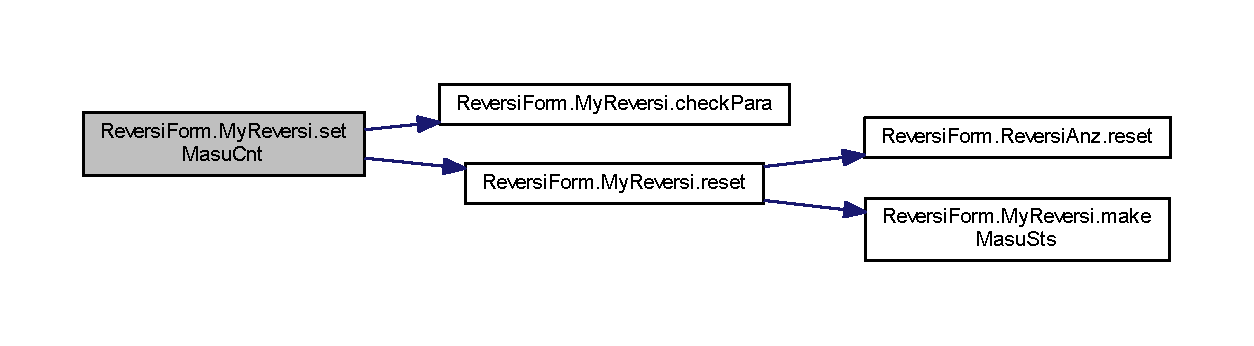
\includegraphics[width=350pt]{class_reversi_form_1_1_my_reversi_af9573f1da0d89180a4dbbd98d41a05fb_cgraph}
\end{center}
\end{figure}
Here is the caller graph for this function\+:
\nopagebreak
\begin{figure}[H]
\begin{center}
\leavevmode
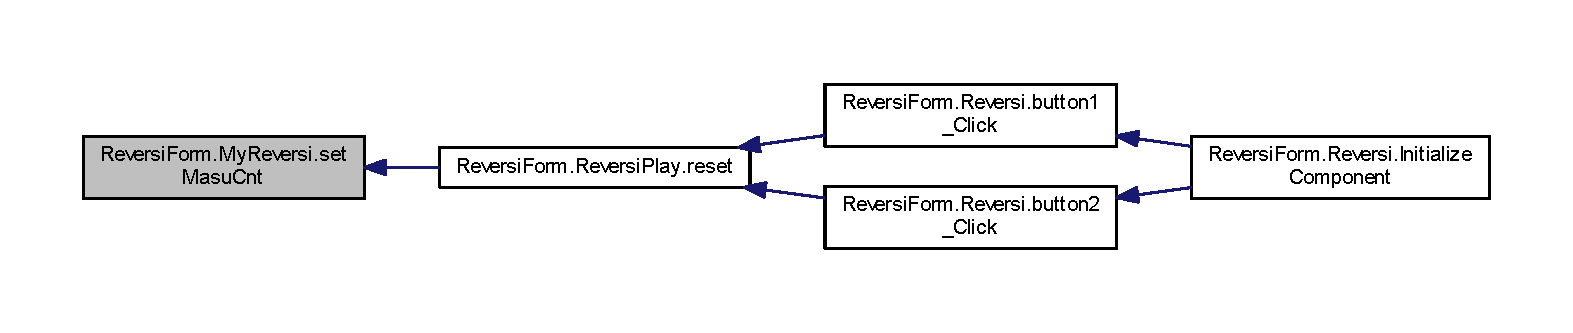
\includegraphics[width=350pt]{class_reversi_form_1_1_my_reversi_af9573f1da0d89180a4dbbd98d41a05fb_icgraph}
\end{center}
\end{figure}
\mbox{\Hypertarget{class_reversi_form_1_1_my_reversi_a1f7ba86f6e8d5dd2fa472a8994e4e3c5}\label{class_reversi_form_1_1_my_reversi_a1f7ba86f6e8d5dd2fa472a8994e4e3c5}} 
\index{Reversi\+Form\+::\+My\+Reversi@{Reversi\+Form\+::\+My\+Reversi}!set\+Masu\+Sts@{set\+Masu\+Sts}}
\index{set\+Masu\+Sts@{set\+Masu\+Sts}!Reversi\+Form\+::\+My\+Reversi@{Reversi\+Form\+::\+My\+Reversi}}
\subsubsection{\texorpdfstring{set\+Masu\+Sts()}{setMasuSts()}}
{\footnotesize\ttfamily int Reversi\+Form.\+My\+Reversi.\+set\+Masu\+Sts (\begin{DoxyParamCaption}\item[{int}]{color,  }\item[{int}]{y,  }\item[{int}]{x }\end{DoxyParamCaption})}



指定座標にコマを置く 


\begin{DoxyParams}[1]{Parameters}
\mbox{\tt in}  & {\em int} & color コマ色 \\
\hline
\mbox{\tt in}  & {\em int} & y マスの\+Y座標 \\
\hline
\mbox{\tt in}  & {\em int} & x マスの\+X座標 \\
\hline
\end{DoxyParams}
\begin{DoxyReturn}{Returns}
0 \+: 成功 それ以外 \+: 失敗 
\end{DoxyReturn}
\begin{DoxyAuthor}{Author}
Yuta Yoshinaga 
\end{DoxyAuthor}
\begin{DoxyDate}{Date}
2017.\+10.\+20 
\end{DoxyDate}


Definition at line 1104 of file My\+Reversi.\+cs.



Referenced by Reversi\+Form.\+Reversi\+Play.\+reset(), Reversi\+Form.\+Reversi\+Play.\+reversi\+Play(), and Reversi\+Form.\+Reversi\+Play.\+reversi\+Play\+Cpu().

Here is the call graph for this function\+:
\nopagebreak
\begin{figure}[H]
\begin{center}
\leavevmode
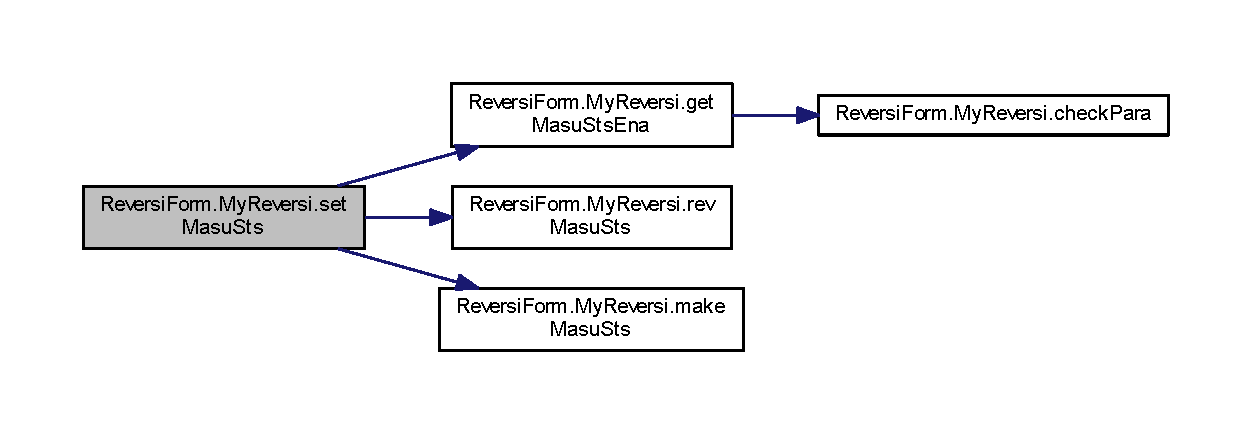
\includegraphics[width=350pt]{class_reversi_form_1_1_my_reversi_a1f7ba86f6e8d5dd2fa472a8994e4e3c5_cgraph}
\end{center}
\end{figure}
Here is the caller graph for this function\+:
\nopagebreak
\begin{figure}[H]
\begin{center}
\leavevmode
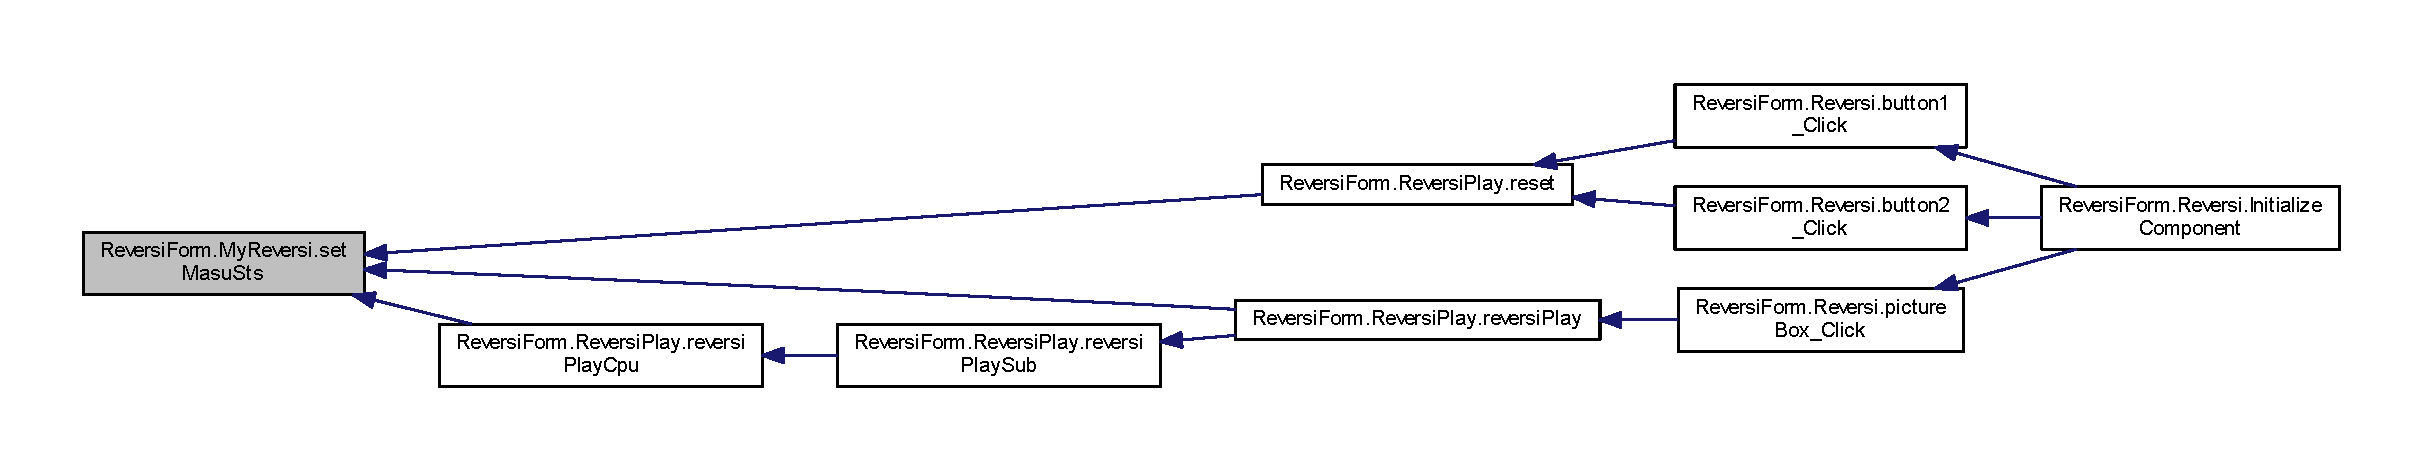
\includegraphics[width=350pt]{class_reversi_form_1_1_my_reversi_a1f7ba86f6e8d5dd2fa472a8994e4e3c5_icgraph}
\end{center}
\end{figure}
\mbox{\Hypertarget{class_reversi_form_1_1_my_reversi_a940c5ec6841ffa050a53276815afcc9d}\label{class_reversi_form_1_1_my_reversi_a940c5ec6841ffa050a53276815afcc9d}} 
\index{Reversi\+Form\+::\+My\+Reversi@{Reversi\+Form\+::\+My\+Reversi}!set\+Masu\+Sts\+Forcibly@{set\+Masu\+Sts\+Forcibly}}
\index{set\+Masu\+Sts\+Forcibly@{set\+Masu\+Sts\+Forcibly}!Reversi\+Form\+::\+My\+Reversi@{Reversi\+Form\+::\+My\+Reversi}}
\subsubsection{\texorpdfstring{set\+Masu\+Sts\+Forcibly()}{setMasuStsForcibly()}}
{\footnotesize\ttfamily int Reversi\+Form.\+My\+Reversi.\+set\+Masu\+Sts\+Forcibly (\begin{DoxyParamCaption}\item[{int}]{color,  }\item[{int}]{y,  }\item[{int}]{x }\end{DoxyParamCaption})}



指定座標にコマを強制的に置く 


\begin{DoxyParams}[1]{Parameters}
\mbox{\tt in}  & {\em int} & color コマ色 \\
\hline
\mbox{\tt in}  & {\em int} & y マスの\+Y座標 \\
\hline
\mbox{\tt in}  & {\em int} & x マスの\+X座標 \\
\hline
\end{DoxyParams}
\begin{DoxyReturn}{Returns}
0 \+: 成功 それ以外 \+: 失敗 
\end{DoxyReturn}
\begin{DoxyAuthor}{Author}
Yuta Yoshinaga 
\end{DoxyAuthor}
\begin{DoxyDate}{Date}
2017.\+10.\+20 
\end{DoxyDate}


Definition at line 1136 of file My\+Reversi.\+cs.



Referenced by Reversi\+Form.\+Reversi\+Play.\+game\+End\+Anim\+Exec().

Here is the caller graph for this function\+:
\nopagebreak
\begin{figure}[H]
\begin{center}
\leavevmode
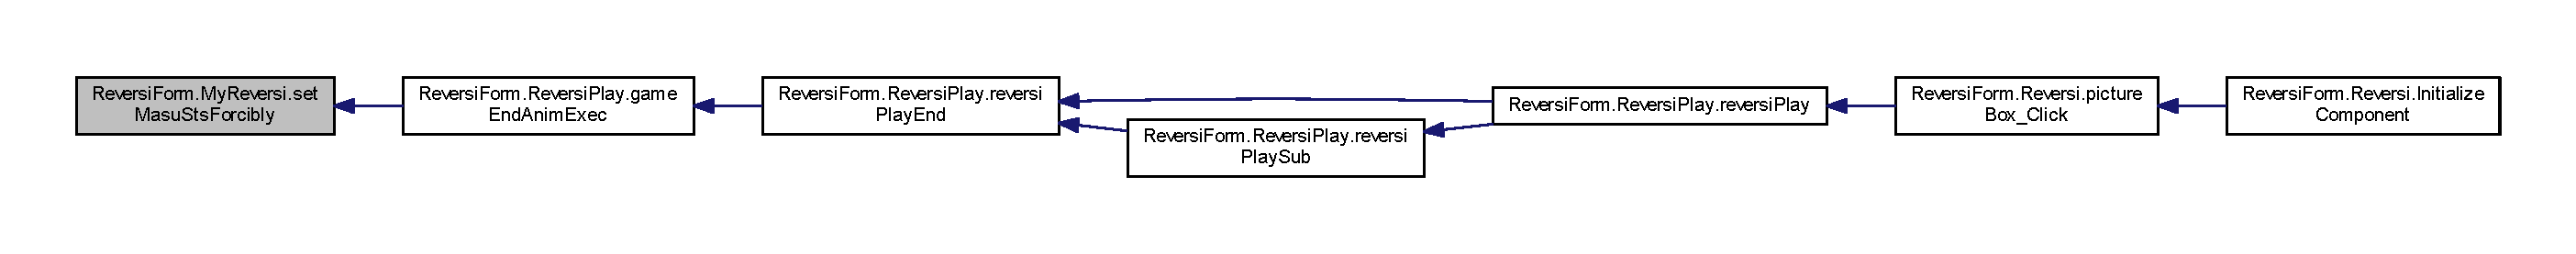
\includegraphics[width=350pt]{class_reversi_form_1_1_my_reversi_a940c5ec6841ffa050a53276815afcc9d_icgraph}
\end{center}
\end{figure}


The documentation for this class was generated from the following file\+:\begin{DoxyCompactItemize}
\item 
Model/\hyperlink{_my_reversi_8cs}{My\+Reversi.\+cs}\end{DoxyCompactItemize}

\hypertarget{class_reversi_form_1_1_program}{}\section{Reversi\+Form.\+Program Class Reference}
\label{class_reversi_form_1_1_program}\index{Reversi\+Form.\+Program@{Reversi\+Form.\+Program}}


Collaboration diagram for Reversi\+Form.\+Program\+:
\nopagebreak
\begin{figure}[H]
\begin{center}
\leavevmode
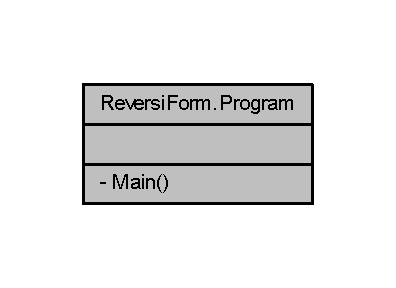
\includegraphics[width=190pt]{class_reversi_form_1_1_program__coll__graph}
\end{center}
\end{figure}
\subsection*{Static Private Member Functions}
\begin{DoxyCompactItemize}
\item 
static void \hyperlink{class_reversi_form_1_1_program_a0d307c8bc3af65198f8bc1cef61e050f}{Main} ()
\begin{DoxyCompactList}\small\item\em アプリケーションのメイン エントリ ポイントです。 \end{DoxyCompactList}\end{DoxyCompactItemize}


\subsection{Detailed Description}


Definition at line 9 of file Program.\+cs.



\subsection{Member Function Documentation}
\mbox{\Hypertarget{class_reversi_form_1_1_program_a0d307c8bc3af65198f8bc1cef61e050f}\label{class_reversi_form_1_1_program_a0d307c8bc3af65198f8bc1cef61e050f}} 
\index{Reversi\+Form\+::\+Program@{Reversi\+Form\+::\+Program}!Main@{Main}}
\index{Main@{Main}!Reversi\+Form\+::\+Program@{Reversi\+Form\+::\+Program}}
\subsubsection{\texorpdfstring{Main()}{Main()}}
{\footnotesize\ttfamily static void Reversi\+Form.\+Program.\+Main (\begin{DoxyParamCaption}{ }\end{DoxyParamCaption})\hspace{0.3cm}{\ttfamily [static]}, {\ttfamily [private]}}



アプリケーションのメイン エントリ ポイントです。 



Definition at line 15 of file Program.\+cs.



The documentation for this class was generated from the following file\+:\begin{DoxyCompactItemize}
\item 
Program.\+cs\end{DoxyCompactItemize}

\hypertarget{class_reversi_form_1_1_reversi}{}\section{Reversi\+Form.\+Reversi Class Reference}
\label{class_reversi_form_1_1_reversi}\index{Reversi\+Form.\+Reversi@{Reversi\+Form.\+Reversi}}


Inheritance diagram for Reversi\+Form.\+Reversi\+:
\nopagebreak
\begin{figure}[H]
\begin{center}
\leavevmode
\includegraphics[height=550pt]{class_reversi_form_1_1_reversi__inherit__graph}
\end{center}
\end{figure}


Collaboration diagram for Reversi\+Form.\+Reversi\+:
\nopagebreak
\begin{figure}[H]
\begin{center}
\leavevmode
\includegraphics[height=550pt]{class_reversi_form_1_1_reversi__coll__graph}
\end{center}
\end{figure}
\subsection*{Public Member Functions}
\begin{DoxyCompactItemize}
\item 
\hyperlink{class_reversi_form_1_1_reversi_setting}{Reversi\+Setting} \hyperlink{class_reversi_form_1_1_reversi_afbe64672e4a4c9e6f6404a3bbf2b5e1d}{Load\+Setting\+Xml} (string path)
\begin{DoxyCompactList}\small\item\em 設定\+X\+M\+Lファイルロード \end{DoxyCompactList}\item 
int \hyperlink{class_reversi_form_1_1_reversi_ac2c2df740914f062761a66f0bbde3f41}{Save\+Setting\+Xml} (string path, ref \hyperlink{class_reversi_form_1_1_reversi_setting}{Reversi\+Setting} app\+Set)
\begin{DoxyCompactList}\small\item\em 設定\+X\+M\+Lファイルセーブ \end{DoxyCompactList}\item 
void \hyperlink{class_reversi_form_1_1_reversi_aab2e35051cbff2f184ee7e76ae60846d}{app\+Init} ()
\begin{DoxyCompactList}\small\item\em アプリ初期化 \end{DoxyCompactList}\item 
void \hyperlink{class_reversi_form_1_1_reversi_af4efb5992bb28d48c4f585a7f6c7906f}{View\+Msg\+Dlg} (string title, string msg)
\begin{DoxyCompactList}\small\item\em メッセージダイアログ \end{DoxyCompactList}\item 
void \hyperlink{class_reversi_form_1_1_reversi_a5b1fd8f327358b4d0551af981b2a7f0c}{View\+Msg\+Dlg\+Local} (string title, string msg)
\begin{DoxyCompactList}\small\item\em メッセージダイアログ \end{DoxyCompactList}\item 
void \hyperlink{class_reversi_form_1_1_reversi_a21483fbe8309e9f6fa5d828fac98a96e}{Draw\+Single} (int y, int x, int sts, int bk, string text)
\begin{DoxyCompactList}\small\item\em 1マス描画 \end{DoxyCompactList}\item 
void \hyperlink{class_reversi_form_1_1_reversi_aaa7228857f9476b7950b0af1524abf44}{Draw\+Single\+Local} (int y, int x, int sts, int bk, string text)
\begin{DoxyCompactList}\small\item\em 1マス描画 \end{DoxyCompactList}\item 
void \hyperlink{class_reversi_form_1_1_reversi_ad09577aef8bf515ee495c82a981dfd7d}{Cur\+Col\+Msg} (string text)
\begin{DoxyCompactList}\small\item\em 現在の色メッセージ \end{DoxyCompactList}\item 
void \hyperlink{class_reversi_form_1_1_reversi_a0d919be21fe5961a177e26b5752320b9}{Cur\+Col\+Msg\+Local} (string text)
\begin{DoxyCompactList}\small\item\em 現在の色メッセージ \end{DoxyCompactList}\item 
void \hyperlink{class_reversi_form_1_1_reversi_af5009aa7b1b255b9dec7028d8a7c53f7}{Cur\+Sts\+Msg} (string text)
\begin{DoxyCompactList}\small\item\em 現在のステータスメッセージ \end{DoxyCompactList}\item 
void \hyperlink{class_reversi_form_1_1_reversi_a934897d68f7709c32b6fd126351c5f05}{Cur\+Sts\+Msg\+Local} (string text)
\begin{DoxyCompactList}\small\item\em 現在のステータスメッセージ \end{DoxyCompactList}\end{DoxyCompactItemize}
\subsection*{Public Attributes}
\begin{DoxyCompactItemize}
\item 
\mbox{\Hypertarget{class_reversi_form_1_1_reversi_ae249a833eae1b8b11e3951d3b27fcba0}\label{class_reversi_form_1_1_reversi_ae249a833eae1b8b11e3951d3b27fcba0}} 
\hyperlink{class_reversi_form_1_1_reversi_setting}{Reversi\+Setting} \hyperlink{class_reversi_form_1_1_reversi_ae249a833eae1b8b11e3951d3b27fcba0}{m\+\_\+\+App\+Settings}
\begin{DoxyCompactList}\small\item\em アプリ設定 \end{DoxyCompactList}\item 
\mbox{\Hypertarget{class_reversi_form_1_1_reversi_a95773c9b8c364a754ca27a4ce8a9bb16}\label{class_reversi_form_1_1_reversi_a95773c9b8c364a754ca27a4ce8a9bb16}} 
\hyperlink{class_reversi_form_1_1_reversi_play}{Reversi\+Play} \hyperlink{class_reversi_form_1_1_reversi_a95773c9b8c364a754ca27a4ce8a9bb16}{m\+\_\+\+Reversi\+Play}
\begin{DoxyCompactList}\small\item\em リバーシ本体 \end{DoxyCompactList}\end{DoxyCompactItemize}
\subsection*{Protected Member Functions}
\begin{DoxyCompactItemize}
\item 
override void \hyperlink{class_reversi_form_1_1_reversi_ac021c14c28e588c11445e460ec7e87d1}{Dispose} (bool disposing)
\begin{DoxyCompactList}\small\item\em 使用中のリソースをすべてクリーンアップします。 \end{DoxyCompactList}\end{DoxyCompactItemize}
\subsection*{Private Member Functions}
\begin{DoxyCompactItemize}
\item 
\mbox{\Hypertarget{class_reversi_form_1_1_reversi_adddf0cf721d71873165e82f67f5d09d8}\label{class_reversi_form_1_1_reversi_adddf0cf721d71873165e82f67f5d09d8}} 
delegate void {\bfseries View\+Msg\+Dlg\+Delegate} (string title, string msg)
\item 
\mbox{\Hypertarget{class_reversi_form_1_1_reversi_a065c6275be5c52e90bdad6fbe8d68362}\label{class_reversi_form_1_1_reversi_a065c6275be5c52e90bdad6fbe8d68362}} 
delegate void {\bfseries Draw\+Single\+Delegate} (int y, int x, int sts, int bk, string text)
\item 
\mbox{\Hypertarget{class_reversi_form_1_1_reversi_abc5c0d998390dc9e9052e514c3824ef6}\label{class_reversi_form_1_1_reversi_abc5c0d998390dc9e9052e514c3824ef6}} 
delegate void {\bfseries Cur\+Col\+Msg\+Delegate} (string text)
\item 
\mbox{\Hypertarget{class_reversi_form_1_1_reversi_a2ed28729afe13d992636e461964e5cd7}\label{class_reversi_form_1_1_reversi_a2ed28729afe13d992636e461964e5cd7}} 
delegate void {\bfseries Cur\+Sts\+Msg\+Delegate} (string text)
\item 
\mbox{\Hypertarget{class_reversi_form_1_1_reversi_a7a4458a4ad3aded3ae17bfe930a122c3}\label{class_reversi_form_1_1_reversi_a7a4458a4ad3aded3ae17bfe930a122c3}} 
delegate void {\bfseries Reversi\+\_\+\+Resize\+End\+Delegate} (object sender, Event\+Args e)
\item 
void \hyperlink{class_reversi_form_1_1_reversi_afaa2a98428f4d9eab723fb71f8cb3e29}{picture\+Box\+\_\+\+Click} (object sender, Event\+Args e)
\begin{DoxyCompactList}\small\item\em マスクリック \end{DoxyCompactList}\item 
void \hyperlink{class_reversi_form_1_1_reversi_a832e3ee4b606141b3feefb47742b3849}{button1\+\_\+\+Click} (object sender, Event\+Args e)
\begin{DoxyCompactList}\small\item\em リセットクリック \end{DoxyCompactList}\item 
void \hyperlink{class_reversi_form_1_1_reversi_aa908556d4f216f8b407c1458e392dfc5}{button2\+\_\+\+Click} (object sender, Event\+Args e)
\begin{DoxyCompactList}\small\item\em セッティングクリック \end{DoxyCompactList}\item 
void \hyperlink{class_reversi_form_1_1_reversi_ac4868f12e6f15387f8f39f5f1934e610}{Reversi\+\_\+\+Resize} (object sender, Event\+Args e)
\begin{DoxyCompactList}\small\item\em リサイズイベント \end{DoxyCompactList}\item 
\mbox{\Hypertarget{class_reversi_form_1_1_reversi_a5b88dc4de7186ee1b04a0619221284a9}\label{class_reversi_form_1_1_reversi_a5b88dc4de7186ee1b04a0619221284a9}} 
void {\bfseries Reversi\+\_\+\+Resize\+End} (object sender, Event\+Args e)
\item 
void \hyperlink{class_reversi_form_1_1_reversi_a7c9ef5ff17c4b888f5c891e3ed5dafc2}{On\+Timed\+Event} (object source, Elapsed\+Event\+Args e)
\begin{DoxyCompactList}\small\item\em タイマーイベント \end{DoxyCompactList}\item 
void \hyperlink{class_reversi_form_1_1_reversi_abec0816dd006d05b512d86b45a20af68}{Initialize\+Component} ()
\begin{DoxyCompactList}\small\item\em デザイナー サポートに必要なメソッドです。このメソッドの内容を コード エディターで変更しないでください。 \end{DoxyCompactList}\end{DoxyCompactItemize}
\subsection*{Private Attributes}
\begin{DoxyCompactItemize}
\item 
\mbox{\Hypertarget{class_reversi_form_1_1_reversi_a4cbca5b82cf5dd63835920c9bc9088b5}\label{class_reversi_form_1_1_reversi_a4cbca5b82cf5dd63835920c9bc9088b5}} 
Size \hyperlink{class_reversi_form_1_1_reversi_a4cbca5b82cf5dd63835920c9bc9088b5}{old\+Size}
\begin{DoxyCompactList}\small\item\em リサイズ前のサイズ \end{DoxyCompactList}\item 
System.\+Component\+Model.\+I\+Container \hyperlink{class_reversi_form_1_1_reversi_a2edc9ab9401997c20553b26aadef1ea0}{components} = null
\begin{DoxyCompactList}\small\item\em 必要なデザイナー変数です。 \end{DoxyCompactList}\item 
\mbox{\Hypertarget{class_reversi_form_1_1_reversi_a9c1a91f97ee65445615b038aca1e72ad}\label{class_reversi_form_1_1_reversi_a9c1a91f97ee65445615b038aca1e72ad}} 
System.\+Windows.\+Forms.\+Table\+Layout\+Panel {\bfseries table\+Layout\+Panel1}
\item 
\mbox{\Hypertarget{class_reversi_form_1_1_reversi_a245193a3e7d97b444dff75302e121d1f}\label{class_reversi_form_1_1_reversi_a245193a3e7d97b444dff75302e121d1f}} 
System.\+Windows.\+Forms.\+Picture\+Box {\bfseries picture\+Box381}
\item 
\mbox{\Hypertarget{class_reversi_form_1_1_reversi_a83ea383942c37ff1e4c8511778944bfb}\label{class_reversi_form_1_1_reversi_a83ea383942c37ff1e4c8511778944bfb}} 
System.\+Windows.\+Forms.\+Picture\+Box {\bfseries picture\+Box382}
\item 
\mbox{\Hypertarget{class_reversi_form_1_1_reversi_ae002f4e7698ce16ade2b501bfdd94186}\label{class_reversi_form_1_1_reversi_ae002f4e7698ce16ade2b501bfdd94186}} 
System.\+Windows.\+Forms.\+Picture\+Box {\bfseries picture\+Box383}
\item 
\mbox{\Hypertarget{class_reversi_form_1_1_reversi_a526f751740d210075b88b4e05e457c73}\label{class_reversi_form_1_1_reversi_a526f751740d210075b88b4e05e457c73}} 
System.\+Windows.\+Forms.\+Picture\+Box {\bfseries picture\+Box384}
\item 
\mbox{\Hypertarget{class_reversi_form_1_1_reversi_ab4812a4de582baba528104b8c5bcc7cf}\label{class_reversi_form_1_1_reversi_ab4812a4de582baba528104b8c5bcc7cf}} 
System.\+Windows.\+Forms.\+Picture\+Box {\bfseries picture\+Box385}
\item 
\mbox{\Hypertarget{class_reversi_form_1_1_reversi_a448c65f41bd162c3365a47a0e0d4a5a1}\label{class_reversi_form_1_1_reversi_a448c65f41bd162c3365a47a0e0d4a5a1}} 
System.\+Windows.\+Forms.\+Picture\+Box {\bfseries picture\+Box386}
\item 
\mbox{\Hypertarget{class_reversi_form_1_1_reversi_a11a439f1b4173f2d256ceb25a44db534}\label{class_reversi_form_1_1_reversi_a11a439f1b4173f2d256ceb25a44db534}} 
System.\+Windows.\+Forms.\+Picture\+Box {\bfseries picture\+Box387}
\item 
\mbox{\Hypertarget{class_reversi_form_1_1_reversi_a8f84dc060240762e9e5b6d346e0a7237}\label{class_reversi_form_1_1_reversi_a8f84dc060240762e9e5b6d346e0a7237}} 
System.\+Windows.\+Forms.\+Picture\+Box {\bfseries picture\+Box388}
\item 
\mbox{\Hypertarget{class_reversi_form_1_1_reversi_a5bdbbd938c48704b9e0aa8f3991a12ac}\label{class_reversi_form_1_1_reversi_a5bdbbd938c48704b9e0aa8f3991a12ac}} 
System.\+Windows.\+Forms.\+Picture\+Box {\bfseries picture\+Box389}
\item 
\mbox{\Hypertarget{class_reversi_form_1_1_reversi_a3f743f1b6070e0589d8315df3ef697ad}\label{class_reversi_form_1_1_reversi_a3f743f1b6070e0589d8315df3ef697ad}} 
System.\+Windows.\+Forms.\+Picture\+Box {\bfseries picture\+Box390}
\item 
\mbox{\Hypertarget{class_reversi_form_1_1_reversi_a4ff9a4c9183b3aa2aae688de04464e07}\label{class_reversi_form_1_1_reversi_a4ff9a4c9183b3aa2aae688de04464e07}} 
System.\+Windows.\+Forms.\+Picture\+Box {\bfseries picture\+Box391}
\item 
\mbox{\Hypertarget{class_reversi_form_1_1_reversi_a593a4e1b0ba2b2dfdf7d3ecb2a70f066}\label{class_reversi_form_1_1_reversi_a593a4e1b0ba2b2dfdf7d3ecb2a70f066}} 
System.\+Windows.\+Forms.\+Picture\+Box {\bfseries picture\+Box392}
\item 
\mbox{\Hypertarget{class_reversi_form_1_1_reversi_a1c6940075e0e83e54e38fe26f1fae9b0}\label{class_reversi_form_1_1_reversi_a1c6940075e0e83e54e38fe26f1fae9b0}} 
System.\+Windows.\+Forms.\+Picture\+Box {\bfseries picture\+Box393}
\item 
\mbox{\Hypertarget{class_reversi_form_1_1_reversi_a63fc4863756d674a6a61c175ff39c732}\label{class_reversi_form_1_1_reversi_a63fc4863756d674a6a61c175ff39c732}} 
System.\+Windows.\+Forms.\+Picture\+Box {\bfseries picture\+Box394}
\item 
\mbox{\Hypertarget{class_reversi_form_1_1_reversi_aa09b880a81de2db3cb4df67098c12271}\label{class_reversi_form_1_1_reversi_aa09b880a81de2db3cb4df67098c12271}} 
System.\+Windows.\+Forms.\+Picture\+Box {\bfseries picture\+Box395}
\item 
\mbox{\Hypertarget{class_reversi_form_1_1_reversi_a816952246abeecb60f720f844c86798f}\label{class_reversi_form_1_1_reversi_a816952246abeecb60f720f844c86798f}} 
System.\+Windows.\+Forms.\+Picture\+Box {\bfseries picture\+Box396}
\item 
\mbox{\Hypertarget{class_reversi_form_1_1_reversi_a1e5db69fde0f6b5bafefa928c4ca6930}\label{class_reversi_form_1_1_reversi_a1e5db69fde0f6b5bafefa928c4ca6930}} 
System.\+Windows.\+Forms.\+Picture\+Box {\bfseries picture\+Box397}
\item 
\mbox{\Hypertarget{class_reversi_form_1_1_reversi_ab5fb1c4484de51870b477b14f2fb5f9b}\label{class_reversi_form_1_1_reversi_ab5fb1c4484de51870b477b14f2fb5f9b}} 
System.\+Windows.\+Forms.\+Picture\+Box {\bfseries picture\+Box398}
\item 
\mbox{\Hypertarget{class_reversi_form_1_1_reversi_a31cd1dca7ce73e2794cd8bbf585a3170}\label{class_reversi_form_1_1_reversi_a31cd1dca7ce73e2794cd8bbf585a3170}} 
System.\+Windows.\+Forms.\+Picture\+Box {\bfseries picture\+Box399}
\item 
\mbox{\Hypertarget{class_reversi_form_1_1_reversi_a4ed0fb9c58c066810ee7bc28683e9b9a}\label{class_reversi_form_1_1_reversi_a4ed0fb9c58c066810ee7bc28683e9b9a}} 
System.\+Windows.\+Forms.\+Picture\+Box {\bfseries picture\+Box400}
\item 
\mbox{\Hypertarget{class_reversi_form_1_1_reversi_aa2e544281ce7ad438ed0ff47af873e6e}\label{class_reversi_form_1_1_reversi_aa2e544281ce7ad438ed0ff47af873e6e}} 
System.\+Windows.\+Forms.\+Picture\+Box {\bfseries picture\+Box361}
\item 
\mbox{\Hypertarget{class_reversi_form_1_1_reversi_a44a0312eaa4b00567750302ebae102f2}\label{class_reversi_form_1_1_reversi_a44a0312eaa4b00567750302ebae102f2}} 
System.\+Windows.\+Forms.\+Picture\+Box {\bfseries picture\+Box362}
\item 
\mbox{\Hypertarget{class_reversi_form_1_1_reversi_aa9a447ddfc05d93c99512935cd20ccf4}\label{class_reversi_form_1_1_reversi_aa9a447ddfc05d93c99512935cd20ccf4}} 
System.\+Windows.\+Forms.\+Picture\+Box {\bfseries picture\+Box363}
\item 
\mbox{\Hypertarget{class_reversi_form_1_1_reversi_ac89c4fb128cbddb938ac7d4d4d3b23e7}\label{class_reversi_form_1_1_reversi_ac89c4fb128cbddb938ac7d4d4d3b23e7}} 
System.\+Windows.\+Forms.\+Picture\+Box {\bfseries picture\+Box364}
\item 
\mbox{\Hypertarget{class_reversi_form_1_1_reversi_a6bf6234f4e2fe58d657c671272b49f7e}\label{class_reversi_form_1_1_reversi_a6bf6234f4e2fe58d657c671272b49f7e}} 
System.\+Windows.\+Forms.\+Picture\+Box {\bfseries picture\+Box365}
\item 
\mbox{\Hypertarget{class_reversi_form_1_1_reversi_a03732708485bb0bc05173165514b2525}\label{class_reversi_form_1_1_reversi_a03732708485bb0bc05173165514b2525}} 
System.\+Windows.\+Forms.\+Picture\+Box {\bfseries picture\+Box366}
\item 
\mbox{\Hypertarget{class_reversi_form_1_1_reversi_a564cb4bce6398b1e4da8019725b70ecc}\label{class_reversi_form_1_1_reversi_a564cb4bce6398b1e4da8019725b70ecc}} 
System.\+Windows.\+Forms.\+Picture\+Box {\bfseries picture\+Box367}
\item 
\mbox{\Hypertarget{class_reversi_form_1_1_reversi_ad07dab1d5586a7f8a212b9934efd07e1}\label{class_reversi_form_1_1_reversi_ad07dab1d5586a7f8a212b9934efd07e1}} 
System.\+Windows.\+Forms.\+Picture\+Box {\bfseries picture\+Box368}
\item 
\mbox{\Hypertarget{class_reversi_form_1_1_reversi_ad1c85204d3a172743e499a8949c1eec9}\label{class_reversi_form_1_1_reversi_ad1c85204d3a172743e499a8949c1eec9}} 
System.\+Windows.\+Forms.\+Picture\+Box {\bfseries picture\+Box369}
\item 
\mbox{\Hypertarget{class_reversi_form_1_1_reversi_a275e503b52c1781c161b63f296bf9fca}\label{class_reversi_form_1_1_reversi_a275e503b52c1781c161b63f296bf9fca}} 
System.\+Windows.\+Forms.\+Picture\+Box {\bfseries picture\+Box370}
\item 
\mbox{\Hypertarget{class_reversi_form_1_1_reversi_ad1e7de51898a4b830492861eccae1e31}\label{class_reversi_form_1_1_reversi_ad1e7de51898a4b830492861eccae1e31}} 
System.\+Windows.\+Forms.\+Picture\+Box {\bfseries picture\+Box371}
\item 
\mbox{\Hypertarget{class_reversi_form_1_1_reversi_ac40745edc0d3942486eb3b69d6474ab5}\label{class_reversi_form_1_1_reversi_ac40745edc0d3942486eb3b69d6474ab5}} 
System.\+Windows.\+Forms.\+Picture\+Box {\bfseries picture\+Box372}
\item 
\mbox{\Hypertarget{class_reversi_form_1_1_reversi_ad67df851a496b4992d3e7663f1716c2f}\label{class_reversi_form_1_1_reversi_ad67df851a496b4992d3e7663f1716c2f}} 
System.\+Windows.\+Forms.\+Picture\+Box {\bfseries picture\+Box373}
\item 
\mbox{\Hypertarget{class_reversi_form_1_1_reversi_a339b27382c564c405d1a70b6c926fca7}\label{class_reversi_form_1_1_reversi_a339b27382c564c405d1a70b6c926fca7}} 
System.\+Windows.\+Forms.\+Picture\+Box {\bfseries picture\+Box374}
\item 
\mbox{\Hypertarget{class_reversi_form_1_1_reversi_a196688ce6db5655628db4ede1cc2fe23}\label{class_reversi_form_1_1_reversi_a196688ce6db5655628db4ede1cc2fe23}} 
System.\+Windows.\+Forms.\+Picture\+Box {\bfseries picture\+Box375}
\item 
\mbox{\Hypertarget{class_reversi_form_1_1_reversi_a00dd5db9cb7f7619b1ff1d866a431b85}\label{class_reversi_form_1_1_reversi_a00dd5db9cb7f7619b1ff1d866a431b85}} 
System.\+Windows.\+Forms.\+Picture\+Box {\bfseries picture\+Box376}
\item 
\mbox{\Hypertarget{class_reversi_form_1_1_reversi_a3e7f5933ccf296bbc4a5081eed277ee5}\label{class_reversi_form_1_1_reversi_a3e7f5933ccf296bbc4a5081eed277ee5}} 
System.\+Windows.\+Forms.\+Picture\+Box {\bfseries picture\+Box377}
\item 
\mbox{\Hypertarget{class_reversi_form_1_1_reversi_aa3c3a913e0a789d9f15ade5ad3d25f9b}\label{class_reversi_form_1_1_reversi_aa3c3a913e0a789d9f15ade5ad3d25f9b}} 
System.\+Windows.\+Forms.\+Picture\+Box {\bfseries picture\+Box378}
\item 
\mbox{\Hypertarget{class_reversi_form_1_1_reversi_af552507643a66288b3c73f56517ad9b9}\label{class_reversi_form_1_1_reversi_af552507643a66288b3c73f56517ad9b9}} 
System.\+Windows.\+Forms.\+Picture\+Box {\bfseries picture\+Box379}
\item 
\mbox{\Hypertarget{class_reversi_form_1_1_reversi_a10de901b585398372895a9e6dad169ae}\label{class_reversi_form_1_1_reversi_a10de901b585398372895a9e6dad169ae}} 
System.\+Windows.\+Forms.\+Picture\+Box {\bfseries picture\+Box380}
\item 
\mbox{\Hypertarget{class_reversi_form_1_1_reversi_a578d70e7659b49189fb4fdf0153b948a}\label{class_reversi_form_1_1_reversi_a578d70e7659b49189fb4fdf0153b948a}} 
System.\+Windows.\+Forms.\+Picture\+Box {\bfseries picture\+Box341}
\item 
\mbox{\Hypertarget{class_reversi_form_1_1_reversi_aec9daa9abb370c7f891e166347aa0b24}\label{class_reversi_form_1_1_reversi_aec9daa9abb370c7f891e166347aa0b24}} 
System.\+Windows.\+Forms.\+Picture\+Box {\bfseries picture\+Box342}
\item 
\mbox{\Hypertarget{class_reversi_form_1_1_reversi_a923188d173a71f0359a22447520ae235}\label{class_reversi_form_1_1_reversi_a923188d173a71f0359a22447520ae235}} 
System.\+Windows.\+Forms.\+Picture\+Box {\bfseries picture\+Box343}
\item 
\mbox{\Hypertarget{class_reversi_form_1_1_reversi_a0ee8620198bcecdb2242557ad0d8167c}\label{class_reversi_form_1_1_reversi_a0ee8620198bcecdb2242557ad0d8167c}} 
System.\+Windows.\+Forms.\+Picture\+Box {\bfseries picture\+Box344}
\item 
\mbox{\Hypertarget{class_reversi_form_1_1_reversi_a99c02398b836e01b7bebe7a390b52fb2}\label{class_reversi_form_1_1_reversi_a99c02398b836e01b7bebe7a390b52fb2}} 
System.\+Windows.\+Forms.\+Picture\+Box {\bfseries picture\+Box345}
\item 
\mbox{\Hypertarget{class_reversi_form_1_1_reversi_ae63fccf78ce858c2617475fbef754072}\label{class_reversi_form_1_1_reversi_ae63fccf78ce858c2617475fbef754072}} 
System.\+Windows.\+Forms.\+Picture\+Box {\bfseries picture\+Box346}
\item 
\mbox{\Hypertarget{class_reversi_form_1_1_reversi_a957792ca1d0808f83ca9a7f417bdad00}\label{class_reversi_form_1_1_reversi_a957792ca1d0808f83ca9a7f417bdad00}} 
System.\+Windows.\+Forms.\+Picture\+Box {\bfseries picture\+Box347}
\item 
\mbox{\Hypertarget{class_reversi_form_1_1_reversi_a8e54e407f78b3c9a79e33b094492be2e}\label{class_reversi_form_1_1_reversi_a8e54e407f78b3c9a79e33b094492be2e}} 
System.\+Windows.\+Forms.\+Picture\+Box {\bfseries picture\+Box348}
\item 
\mbox{\Hypertarget{class_reversi_form_1_1_reversi_aecd5c3382d0c3b7ddf1abf3c34b0553c}\label{class_reversi_form_1_1_reversi_aecd5c3382d0c3b7ddf1abf3c34b0553c}} 
System.\+Windows.\+Forms.\+Picture\+Box {\bfseries picture\+Box349}
\item 
\mbox{\Hypertarget{class_reversi_form_1_1_reversi_a63f17bcc9584f62ee1a1ffca3365e808}\label{class_reversi_form_1_1_reversi_a63f17bcc9584f62ee1a1ffca3365e808}} 
System.\+Windows.\+Forms.\+Picture\+Box {\bfseries picture\+Box350}
\item 
\mbox{\Hypertarget{class_reversi_form_1_1_reversi_a65c6093716b888636e9a97f6c779b420}\label{class_reversi_form_1_1_reversi_a65c6093716b888636e9a97f6c779b420}} 
System.\+Windows.\+Forms.\+Picture\+Box {\bfseries picture\+Box351}
\item 
\mbox{\Hypertarget{class_reversi_form_1_1_reversi_a33e817c72db19c9355717ce5cfa10623}\label{class_reversi_form_1_1_reversi_a33e817c72db19c9355717ce5cfa10623}} 
System.\+Windows.\+Forms.\+Picture\+Box {\bfseries picture\+Box352}
\item 
\mbox{\Hypertarget{class_reversi_form_1_1_reversi_aaf509a925a44d92e5e93f9224f818157}\label{class_reversi_form_1_1_reversi_aaf509a925a44d92e5e93f9224f818157}} 
System.\+Windows.\+Forms.\+Picture\+Box {\bfseries picture\+Box353}
\item 
\mbox{\Hypertarget{class_reversi_form_1_1_reversi_ac2a95597ead8c77092658f0d98f3e0bc}\label{class_reversi_form_1_1_reversi_ac2a95597ead8c77092658f0d98f3e0bc}} 
System.\+Windows.\+Forms.\+Picture\+Box {\bfseries picture\+Box354}
\item 
\mbox{\Hypertarget{class_reversi_form_1_1_reversi_af9cb362053e97ac3201d452b9e6e3e24}\label{class_reversi_form_1_1_reversi_af9cb362053e97ac3201d452b9e6e3e24}} 
System.\+Windows.\+Forms.\+Picture\+Box {\bfseries picture\+Box355}
\item 
\mbox{\Hypertarget{class_reversi_form_1_1_reversi_af34d5cc89c9b861df0949ce370df20ab}\label{class_reversi_form_1_1_reversi_af34d5cc89c9b861df0949ce370df20ab}} 
System.\+Windows.\+Forms.\+Picture\+Box {\bfseries picture\+Box356}
\item 
\mbox{\Hypertarget{class_reversi_form_1_1_reversi_ac23cbc926c88e13a970519efbc7de75c}\label{class_reversi_form_1_1_reversi_ac23cbc926c88e13a970519efbc7de75c}} 
System.\+Windows.\+Forms.\+Picture\+Box {\bfseries picture\+Box357}
\item 
\mbox{\Hypertarget{class_reversi_form_1_1_reversi_a30addbb35760e76979aa0d251a782313}\label{class_reversi_form_1_1_reversi_a30addbb35760e76979aa0d251a782313}} 
System.\+Windows.\+Forms.\+Picture\+Box {\bfseries picture\+Box358}
\item 
\mbox{\Hypertarget{class_reversi_form_1_1_reversi_afb35bc7a27fe4f41da041ca39ed94c04}\label{class_reversi_form_1_1_reversi_afb35bc7a27fe4f41da041ca39ed94c04}} 
System.\+Windows.\+Forms.\+Picture\+Box {\bfseries picture\+Box359}
\item 
\mbox{\Hypertarget{class_reversi_form_1_1_reversi_ad7b4c8f3c4aa7aa67f2d81d804a5fc9a}\label{class_reversi_form_1_1_reversi_ad7b4c8f3c4aa7aa67f2d81d804a5fc9a}} 
System.\+Windows.\+Forms.\+Picture\+Box {\bfseries picture\+Box360}
\item 
\mbox{\Hypertarget{class_reversi_form_1_1_reversi_a67abeeffca08c0897399bc95d373732f}\label{class_reversi_form_1_1_reversi_a67abeeffca08c0897399bc95d373732f}} 
System.\+Windows.\+Forms.\+Picture\+Box {\bfseries picture\+Box321}
\item 
\mbox{\Hypertarget{class_reversi_form_1_1_reversi_a8a1a09809422bc4b0b1b8fc42b6d5b0a}\label{class_reversi_form_1_1_reversi_a8a1a09809422bc4b0b1b8fc42b6d5b0a}} 
System.\+Windows.\+Forms.\+Picture\+Box {\bfseries picture\+Box322}
\item 
\mbox{\Hypertarget{class_reversi_form_1_1_reversi_a2be16f32e873c08f603c0d7a17bb1e93}\label{class_reversi_form_1_1_reversi_a2be16f32e873c08f603c0d7a17bb1e93}} 
System.\+Windows.\+Forms.\+Picture\+Box {\bfseries picture\+Box323}
\item 
\mbox{\Hypertarget{class_reversi_form_1_1_reversi_a57e5cd2d833faf315f38d56ba6706ec0}\label{class_reversi_form_1_1_reversi_a57e5cd2d833faf315f38d56ba6706ec0}} 
System.\+Windows.\+Forms.\+Picture\+Box {\bfseries picture\+Box324}
\item 
\mbox{\Hypertarget{class_reversi_form_1_1_reversi_a59da237a9ff6e757855439f1ba20260b}\label{class_reversi_form_1_1_reversi_a59da237a9ff6e757855439f1ba20260b}} 
System.\+Windows.\+Forms.\+Picture\+Box {\bfseries picture\+Box325}
\item 
\mbox{\Hypertarget{class_reversi_form_1_1_reversi_aa488a676f3079b7b7b81e12ad75c8057}\label{class_reversi_form_1_1_reversi_aa488a676f3079b7b7b81e12ad75c8057}} 
System.\+Windows.\+Forms.\+Picture\+Box {\bfseries picture\+Box326}
\item 
\mbox{\Hypertarget{class_reversi_form_1_1_reversi_aaaa72d48cecc5132b2eae956b675de63}\label{class_reversi_form_1_1_reversi_aaaa72d48cecc5132b2eae956b675de63}} 
System.\+Windows.\+Forms.\+Picture\+Box {\bfseries picture\+Box327}
\item 
\mbox{\Hypertarget{class_reversi_form_1_1_reversi_ab4bc48e71ab518c31643046da106aa39}\label{class_reversi_form_1_1_reversi_ab4bc48e71ab518c31643046da106aa39}} 
System.\+Windows.\+Forms.\+Picture\+Box {\bfseries picture\+Box328}
\item 
\mbox{\Hypertarget{class_reversi_form_1_1_reversi_a841d83d77486c9ad086400d277e8d4ad}\label{class_reversi_form_1_1_reversi_a841d83d77486c9ad086400d277e8d4ad}} 
System.\+Windows.\+Forms.\+Picture\+Box {\bfseries picture\+Box329}
\item 
\mbox{\Hypertarget{class_reversi_form_1_1_reversi_a4fd063fb31960cde998b47be4d17d793}\label{class_reversi_form_1_1_reversi_a4fd063fb31960cde998b47be4d17d793}} 
System.\+Windows.\+Forms.\+Picture\+Box {\bfseries picture\+Box330}
\item 
\mbox{\Hypertarget{class_reversi_form_1_1_reversi_adc3296857dac7e9d46618df201107906}\label{class_reversi_form_1_1_reversi_adc3296857dac7e9d46618df201107906}} 
System.\+Windows.\+Forms.\+Picture\+Box {\bfseries picture\+Box331}
\item 
\mbox{\Hypertarget{class_reversi_form_1_1_reversi_a108893bc3c675b0437921cfdd4dac7c7}\label{class_reversi_form_1_1_reversi_a108893bc3c675b0437921cfdd4dac7c7}} 
System.\+Windows.\+Forms.\+Picture\+Box {\bfseries picture\+Box332}
\item 
\mbox{\Hypertarget{class_reversi_form_1_1_reversi_af30b7b18ec3f3048e210bfe981897d77}\label{class_reversi_form_1_1_reversi_af30b7b18ec3f3048e210bfe981897d77}} 
System.\+Windows.\+Forms.\+Picture\+Box {\bfseries picture\+Box333}
\item 
\mbox{\Hypertarget{class_reversi_form_1_1_reversi_a48f3ed9b7bc3c972761d914b3cf93c52}\label{class_reversi_form_1_1_reversi_a48f3ed9b7bc3c972761d914b3cf93c52}} 
System.\+Windows.\+Forms.\+Picture\+Box {\bfseries picture\+Box334}
\item 
\mbox{\Hypertarget{class_reversi_form_1_1_reversi_a6f89a77d0acbdc9a31a11feda5c607df}\label{class_reversi_form_1_1_reversi_a6f89a77d0acbdc9a31a11feda5c607df}} 
System.\+Windows.\+Forms.\+Picture\+Box {\bfseries picture\+Box335}
\item 
\mbox{\Hypertarget{class_reversi_form_1_1_reversi_a7859c6e89c448fbe0e89f222049608a0}\label{class_reversi_form_1_1_reversi_a7859c6e89c448fbe0e89f222049608a0}} 
System.\+Windows.\+Forms.\+Picture\+Box {\bfseries picture\+Box336}
\item 
\mbox{\Hypertarget{class_reversi_form_1_1_reversi_a2a096174503f5f1df105da9b0959fda2}\label{class_reversi_form_1_1_reversi_a2a096174503f5f1df105da9b0959fda2}} 
System.\+Windows.\+Forms.\+Picture\+Box {\bfseries picture\+Box337}
\item 
\mbox{\Hypertarget{class_reversi_form_1_1_reversi_ad6c05b746370ab3505409ef7f8072afd}\label{class_reversi_form_1_1_reversi_ad6c05b746370ab3505409ef7f8072afd}} 
System.\+Windows.\+Forms.\+Picture\+Box {\bfseries picture\+Box338}
\item 
\mbox{\Hypertarget{class_reversi_form_1_1_reversi_af60aa0a600492db838105c04e5949911}\label{class_reversi_form_1_1_reversi_af60aa0a600492db838105c04e5949911}} 
System.\+Windows.\+Forms.\+Picture\+Box {\bfseries picture\+Box339}
\item 
\mbox{\Hypertarget{class_reversi_form_1_1_reversi_a2e922a2d7fc5269a73103ae64834266c}\label{class_reversi_form_1_1_reversi_a2e922a2d7fc5269a73103ae64834266c}} 
System.\+Windows.\+Forms.\+Picture\+Box {\bfseries picture\+Box340}
\item 
\mbox{\Hypertarget{class_reversi_form_1_1_reversi_a30f563f5c04502beb3d93535fc17ae32}\label{class_reversi_form_1_1_reversi_a30f563f5c04502beb3d93535fc17ae32}} 
System.\+Windows.\+Forms.\+Picture\+Box {\bfseries picture\+Box301}
\item 
\mbox{\Hypertarget{class_reversi_form_1_1_reversi_ac95b75a3c2b0064b287edd93924d3cef}\label{class_reversi_form_1_1_reversi_ac95b75a3c2b0064b287edd93924d3cef}} 
System.\+Windows.\+Forms.\+Picture\+Box {\bfseries picture\+Box302}
\item 
\mbox{\Hypertarget{class_reversi_form_1_1_reversi_a75eb83d40fefbfc13a5012535fd1bffe}\label{class_reversi_form_1_1_reversi_a75eb83d40fefbfc13a5012535fd1bffe}} 
System.\+Windows.\+Forms.\+Picture\+Box {\bfseries picture\+Box303}
\item 
\mbox{\Hypertarget{class_reversi_form_1_1_reversi_ab329757fbe09ca5ac10b1e0c527ce6dc}\label{class_reversi_form_1_1_reversi_ab329757fbe09ca5ac10b1e0c527ce6dc}} 
System.\+Windows.\+Forms.\+Picture\+Box {\bfseries picture\+Box304}
\item 
\mbox{\Hypertarget{class_reversi_form_1_1_reversi_a7c68afbdc7ac0d4d1a2aa9dea4b81c66}\label{class_reversi_form_1_1_reversi_a7c68afbdc7ac0d4d1a2aa9dea4b81c66}} 
System.\+Windows.\+Forms.\+Picture\+Box {\bfseries picture\+Box305}
\item 
\mbox{\Hypertarget{class_reversi_form_1_1_reversi_ace31163ed6e4ee4baff20b2e3252c4a3}\label{class_reversi_form_1_1_reversi_ace31163ed6e4ee4baff20b2e3252c4a3}} 
System.\+Windows.\+Forms.\+Picture\+Box {\bfseries picture\+Box306}
\item 
\mbox{\Hypertarget{class_reversi_form_1_1_reversi_acff75778dc8e71856fc46e29d3c5c6f3}\label{class_reversi_form_1_1_reversi_acff75778dc8e71856fc46e29d3c5c6f3}} 
System.\+Windows.\+Forms.\+Picture\+Box {\bfseries picture\+Box307}
\item 
\mbox{\Hypertarget{class_reversi_form_1_1_reversi_add4aa1d43afab596720a5b163a909e7d}\label{class_reversi_form_1_1_reversi_add4aa1d43afab596720a5b163a909e7d}} 
System.\+Windows.\+Forms.\+Picture\+Box {\bfseries picture\+Box308}
\item 
\mbox{\Hypertarget{class_reversi_form_1_1_reversi_a57384c67de7f6c5402747b21216aacea}\label{class_reversi_form_1_1_reversi_a57384c67de7f6c5402747b21216aacea}} 
System.\+Windows.\+Forms.\+Picture\+Box {\bfseries picture\+Box309}
\item 
\mbox{\Hypertarget{class_reversi_form_1_1_reversi_aca109e4cfb03e75521ba7fb05aa490eb}\label{class_reversi_form_1_1_reversi_aca109e4cfb03e75521ba7fb05aa490eb}} 
System.\+Windows.\+Forms.\+Picture\+Box {\bfseries picture\+Box310}
\item 
\mbox{\Hypertarget{class_reversi_form_1_1_reversi_a82d1e8e581cd413a43b1b50bb1f8bfe0}\label{class_reversi_form_1_1_reversi_a82d1e8e581cd413a43b1b50bb1f8bfe0}} 
System.\+Windows.\+Forms.\+Picture\+Box {\bfseries picture\+Box311}
\item 
\mbox{\Hypertarget{class_reversi_form_1_1_reversi_af6d35eb27e98b5029a1a153f99961f09}\label{class_reversi_form_1_1_reversi_af6d35eb27e98b5029a1a153f99961f09}} 
System.\+Windows.\+Forms.\+Picture\+Box {\bfseries picture\+Box312}
\item 
\mbox{\Hypertarget{class_reversi_form_1_1_reversi_ace2e9da7a5ab52911524271c680c8dd4}\label{class_reversi_form_1_1_reversi_ace2e9da7a5ab52911524271c680c8dd4}} 
System.\+Windows.\+Forms.\+Picture\+Box {\bfseries picture\+Box313}
\item 
\mbox{\Hypertarget{class_reversi_form_1_1_reversi_a9fb3214a6c48868c43d9447b7804733d}\label{class_reversi_form_1_1_reversi_a9fb3214a6c48868c43d9447b7804733d}} 
System.\+Windows.\+Forms.\+Picture\+Box {\bfseries picture\+Box314}
\item 
\mbox{\Hypertarget{class_reversi_form_1_1_reversi_a1d072e81561aa5eb609f108af6f320c5}\label{class_reversi_form_1_1_reversi_a1d072e81561aa5eb609f108af6f320c5}} 
System.\+Windows.\+Forms.\+Picture\+Box {\bfseries picture\+Box315}
\item 
\mbox{\Hypertarget{class_reversi_form_1_1_reversi_a4480af038b6431446c2a3c6b6c4a68a1}\label{class_reversi_form_1_1_reversi_a4480af038b6431446c2a3c6b6c4a68a1}} 
System.\+Windows.\+Forms.\+Picture\+Box {\bfseries picture\+Box316}
\item 
\mbox{\Hypertarget{class_reversi_form_1_1_reversi_a23adc8e49e28dcef35be06bd3bc81d11}\label{class_reversi_form_1_1_reversi_a23adc8e49e28dcef35be06bd3bc81d11}} 
System.\+Windows.\+Forms.\+Picture\+Box {\bfseries picture\+Box317}
\item 
\mbox{\Hypertarget{class_reversi_form_1_1_reversi_ace37ca088cc0c266b7a80faba81eb9d4}\label{class_reversi_form_1_1_reversi_ace37ca088cc0c266b7a80faba81eb9d4}} 
System.\+Windows.\+Forms.\+Picture\+Box {\bfseries picture\+Box318}
\item 
\mbox{\Hypertarget{class_reversi_form_1_1_reversi_a3833d3c665906310078b1708727a3c63}\label{class_reversi_form_1_1_reversi_a3833d3c665906310078b1708727a3c63}} 
System.\+Windows.\+Forms.\+Picture\+Box {\bfseries picture\+Box319}
\item 
\mbox{\Hypertarget{class_reversi_form_1_1_reversi_a16dcebac8ac18640b4e7cb557032cc65}\label{class_reversi_form_1_1_reversi_a16dcebac8ac18640b4e7cb557032cc65}} 
System.\+Windows.\+Forms.\+Picture\+Box {\bfseries picture\+Box320}
\item 
\mbox{\Hypertarget{class_reversi_form_1_1_reversi_a8a83c9b9879c855f934dc473de383c8f}\label{class_reversi_form_1_1_reversi_a8a83c9b9879c855f934dc473de383c8f}} 
System.\+Windows.\+Forms.\+Picture\+Box {\bfseries picture\+Box281}
\item 
\mbox{\Hypertarget{class_reversi_form_1_1_reversi_a59cfa525157acd51b61bc7a1a1e77853}\label{class_reversi_form_1_1_reversi_a59cfa525157acd51b61bc7a1a1e77853}} 
System.\+Windows.\+Forms.\+Picture\+Box {\bfseries picture\+Box282}
\item 
\mbox{\Hypertarget{class_reversi_form_1_1_reversi_a3576a78dec2fce91578dc2b881ce0d34}\label{class_reversi_form_1_1_reversi_a3576a78dec2fce91578dc2b881ce0d34}} 
System.\+Windows.\+Forms.\+Picture\+Box {\bfseries picture\+Box283}
\item 
\mbox{\Hypertarget{class_reversi_form_1_1_reversi_a5402a2050897d23a62018ee0d7fef0ee}\label{class_reversi_form_1_1_reversi_a5402a2050897d23a62018ee0d7fef0ee}} 
System.\+Windows.\+Forms.\+Picture\+Box {\bfseries picture\+Box284}
\item 
\mbox{\Hypertarget{class_reversi_form_1_1_reversi_a6308c8bf2ffc8b1fb4c2bcfba5b042e3}\label{class_reversi_form_1_1_reversi_a6308c8bf2ffc8b1fb4c2bcfba5b042e3}} 
System.\+Windows.\+Forms.\+Picture\+Box {\bfseries picture\+Box285}
\item 
\mbox{\Hypertarget{class_reversi_form_1_1_reversi_a4e5c410e6af7bce0370e5aff8f11f4e1}\label{class_reversi_form_1_1_reversi_a4e5c410e6af7bce0370e5aff8f11f4e1}} 
System.\+Windows.\+Forms.\+Picture\+Box {\bfseries picture\+Box286}
\item 
\mbox{\Hypertarget{class_reversi_form_1_1_reversi_a391c9668ba85274262e9b457bdf3d13e}\label{class_reversi_form_1_1_reversi_a391c9668ba85274262e9b457bdf3d13e}} 
System.\+Windows.\+Forms.\+Picture\+Box {\bfseries picture\+Box287}
\item 
\mbox{\Hypertarget{class_reversi_form_1_1_reversi_a0c7235b4e3921531d0c8bb0d9b87a525}\label{class_reversi_form_1_1_reversi_a0c7235b4e3921531d0c8bb0d9b87a525}} 
System.\+Windows.\+Forms.\+Picture\+Box {\bfseries picture\+Box288}
\item 
\mbox{\Hypertarget{class_reversi_form_1_1_reversi_af068e9343b271d21e152a6b766070e38}\label{class_reversi_form_1_1_reversi_af068e9343b271d21e152a6b766070e38}} 
System.\+Windows.\+Forms.\+Picture\+Box {\bfseries picture\+Box289}
\item 
\mbox{\Hypertarget{class_reversi_form_1_1_reversi_a321c0df794bb7dc31ef04cc5bd8ff0da}\label{class_reversi_form_1_1_reversi_a321c0df794bb7dc31ef04cc5bd8ff0da}} 
System.\+Windows.\+Forms.\+Picture\+Box {\bfseries picture\+Box290}
\item 
\mbox{\Hypertarget{class_reversi_form_1_1_reversi_aea82e5d8c816e49bdd6797b58ec2bf11}\label{class_reversi_form_1_1_reversi_aea82e5d8c816e49bdd6797b58ec2bf11}} 
System.\+Windows.\+Forms.\+Picture\+Box {\bfseries picture\+Box291}
\item 
\mbox{\Hypertarget{class_reversi_form_1_1_reversi_abd429145542eb929e981637a63a4d9b4}\label{class_reversi_form_1_1_reversi_abd429145542eb929e981637a63a4d9b4}} 
System.\+Windows.\+Forms.\+Picture\+Box {\bfseries picture\+Box292}
\item 
\mbox{\Hypertarget{class_reversi_form_1_1_reversi_ae6acbfbf80ed7cfe3b166167313d487d}\label{class_reversi_form_1_1_reversi_ae6acbfbf80ed7cfe3b166167313d487d}} 
System.\+Windows.\+Forms.\+Picture\+Box {\bfseries picture\+Box293}
\item 
\mbox{\Hypertarget{class_reversi_form_1_1_reversi_a5039a5854e6d1cbaa1c61213e71db8b4}\label{class_reversi_form_1_1_reversi_a5039a5854e6d1cbaa1c61213e71db8b4}} 
System.\+Windows.\+Forms.\+Picture\+Box {\bfseries picture\+Box294}
\item 
\mbox{\Hypertarget{class_reversi_form_1_1_reversi_a70773c9368b5bac9952be75c570ce3d9}\label{class_reversi_form_1_1_reversi_a70773c9368b5bac9952be75c570ce3d9}} 
System.\+Windows.\+Forms.\+Picture\+Box {\bfseries picture\+Box295}
\item 
\mbox{\Hypertarget{class_reversi_form_1_1_reversi_a9182f211b6e2a59a62d25660efc2a72d}\label{class_reversi_form_1_1_reversi_a9182f211b6e2a59a62d25660efc2a72d}} 
System.\+Windows.\+Forms.\+Picture\+Box {\bfseries picture\+Box296}
\item 
\mbox{\Hypertarget{class_reversi_form_1_1_reversi_af938f24d4ef565e2abe00502363a149b}\label{class_reversi_form_1_1_reversi_af938f24d4ef565e2abe00502363a149b}} 
System.\+Windows.\+Forms.\+Picture\+Box {\bfseries picture\+Box297}
\item 
\mbox{\Hypertarget{class_reversi_form_1_1_reversi_af67d2f91fc32f5793ebc5a857949d990}\label{class_reversi_form_1_1_reversi_af67d2f91fc32f5793ebc5a857949d990}} 
System.\+Windows.\+Forms.\+Picture\+Box {\bfseries picture\+Box298}
\item 
\mbox{\Hypertarget{class_reversi_form_1_1_reversi_aa27c749a23a913ee2147f80aa674c853}\label{class_reversi_form_1_1_reversi_aa27c749a23a913ee2147f80aa674c853}} 
System.\+Windows.\+Forms.\+Picture\+Box {\bfseries picture\+Box299}
\item 
\mbox{\Hypertarget{class_reversi_form_1_1_reversi_afcbc8c3d887fd9918ee02faa8b742e23}\label{class_reversi_form_1_1_reversi_afcbc8c3d887fd9918ee02faa8b742e23}} 
System.\+Windows.\+Forms.\+Picture\+Box {\bfseries picture\+Box300}
\item 
\mbox{\Hypertarget{class_reversi_form_1_1_reversi_a56a1519fdaf8ae3b89c8a575cf2bc86f}\label{class_reversi_form_1_1_reversi_a56a1519fdaf8ae3b89c8a575cf2bc86f}} 
System.\+Windows.\+Forms.\+Picture\+Box {\bfseries picture\+Box261}
\item 
\mbox{\Hypertarget{class_reversi_form_1_1_reversi_a68f7e531e00903aff993775f579d2dc0}\label{class_reversi_form_1_1_reversi_a68f7e531e00903aff993775f579d2dc0}} 
System.\+Windows.\+Forms.\+Picture\+Box {\bfseries picture\+Box262}
\item 
\mbox{\Hypertarget{class_reversi_form_1_1_reversi_a7b32307a1d95fe7415d7162b688a2f2c}\label{class_reversi_form_1_1_reversi_a7b32307a1d95fe7415d7162b688a2f2c}} 
System.\+Windows.\+Forms.\+Picture\+Box {\bfseries picture\+Box263}
\item 
\mbox{\Hypertarget{class_reversi_form_1_1_reversi_a19163c241bad62f8888717cd7e6def94}\label{class_reversi_form_1_1_reversi_a19163c241bad62f8888717cd7e6def94}} 
System.\+Windows.\+Forms.\+Picture\+Box {\bfseries picture\+Box264}
\item 
\mbox{\Hypertarget{class_reversi_form_1_1_reversi_a7d9316a95394667be921de9b9dab488f}\label{class_reversi_form_1_1_reversi_a7d9316a95394667be921de9b9dab488f}} 
System.\+Windows.\+Forms.\+Picture\+Box {\bfseries picture\+Box265}
\item 
\mbox{\Hypertarget{class_reversi_form_1_1_reversi_a460b9119a6884844e8103eb81020a1b4}\label{class_reversi_form_1_1_reversi_a460b9119a6884844e8103eb81020a1b4}} 
System.\+Windows.\+Forms.\+Picture\+Box {\bfseries picture\+Box266}
\item 
\mbox{\Hypertarget{class_reversi_form_1_1_reversi_a4537c39c6d5f345198ebf9b45ec7a07e}\label{class_reversi_form_1_1_reversi_a4537c39c6d5f345198ebf9b45ec7a07e}} 
System.\+Windows.\+Forms.\+Picture\+Box {\bfseries picture\+Box267}
\item 
\mbox{\Hypertarget{class_reversi_form_1_1_reversi_a63abe94b9251fd607e2c6c24dccd8b5a}\label{class_reversi_form_1_1_reversi_a63abe94b9251fd607e2c6c24dccd8b5a}} 
System.\+Windows.\+Forms.\+Picture\+Box {\bfseries picture\+Box268}
\item 
\mbox{\Hypertarget{class_reversi_form_1_1_reversi_a0463f0292d5332589a4ba2afb6b86e7e}\label{class_reversi_form_1_1_reversi_a0463f0292d5332589a4ba2afb6b86e7e}} 
System.\+Windows.\+Forms.\+Picture\+Box {\bfseries picture\+Box269}
\item 
\mbox{\Hypertarget{class_reversi_form_1_1_reversi_aaad641bcdfbf3e4a5aec89a3063cafd9}\label{class_reversi_form_1_1_reversi_aaad641bcdfbf3e4a5aec89a3063cafd9}} 
System.\+Windows.\+Forms.\+Picture\+Box {\bfseries picture\+Box270}
\item 
\mbox{\Hypertarget{class_reversi_form_1_1_reversi_a7415fbe3b1d77f78c85a9f2f011ab135}\label{class_reversi_form_1_1_reversi_a7415fbe3b1d77f78c85a9f2f011ab135}} 
System.\+Windows.\+Forms.\+Picture\+Box {\bfseries picture\+Box271}
\item 
\mbox{\Hypertarget{class_reversi_form_1_1_reversi_a4cc5e78418af588f845ea66d308b62c7}\label{class_reversi_form_1_1_reversi_a4cc5e78418af588f845ea66d308b62c7}} 
System.\+Windows.\+Forms.\+Picture\+Box {\bfseries picture\+Box272}
\item 
\mbox{\Hypertarget{class_reversi_form_1_1_reversi_a2320555e3cbbe02353e3401046233896}\label{class_reversi_form_1_1_reversi_a2320555e3cbbe02353e3401046233896}} 
System.\+Windows.\+Forms.\+Picture\+Box {\bfseries picture\+Box273}
\item 
\mbox{\Hypertarget{class_reversi_form_1_1_reversi_a7c0a88ad3b5790db20940a0ad876b2b5}\label{class_reversi_form_1_1_reversi_a7c0a88ad3b5790db20940a0ad876b2b5}} 
System.\+Windows.\+Forms.\+Picture\+Box {\bfseries picture\+Box274}
\item 
\mbox{\Hypertarget{class_reversi_form_1_1_reversi_ac27cfe52a20dc14d4200f5c1a56cc977}\label{class_reversi_form_1_1_reversi_ac27cfe52a20dc14d4200f5c1a56cc977}} 
System.\+Windows.\+Forms.\+Picture\+Box {\bfseries picture\+Box275}
\item 
\mbox{\Hypertarget{class_reversi_form_1_1_reversi_a376c210284e9e1fd656a88ae99bd7b49}\label{class_reversi_form_1_1_reversi_a376c210284e9e1fd656a88ae99bd7b49}} 
System.\+Windows.\+Forms.\+Picture\+Box {\bfseries picture\+Box276}
\item 
\mbox{\Hypertarget{class_reversi_form_1_1_reversi_a93dc4329d7f5fb65154f5460ac018d37}\label{class_reversi_form_1_1_reversi_a93dc4329d7f5fb65154f5460ac018d37}} 
System.\+Windows.\+Forms.\+Picture\+Box {\bfseries picture\+Box277}
\item 
\mbox{\Hypertarget{class_reversi_form_1_1_reversi_abf0bc1296a9e987914befdea40f788f2}\label{class_reversi_form_1_1_reversi_abf0bc1296a9e987914befdea40f788f2}} 
System.\+Windows.\+Forms.\+Picture\+Box {\bfseries picture\+Box278}
\item 
\mbox{\Hypertarget{class_reversi_form_1_1_reversi_ab776c972d1afed2dd84fde600eb3ed6a}\label{class_reversi_form_1_1_reversi_ab776c972d1afed2dd84fde600eb3ed6a}} 
System.\+Windows.\+Forms.\+Picture\+Box {\bfseries picture\+Box279}
\item 
\mbox{\Hypertarget{class_reversi_form_1_1_reversi_ae16ca4cf745ad1f08a0387ae098cbf8b}\label{class_reversi_form_1_1_reversi_ae16ca4cf745ad1f08a0387ae098cbf8b}} 
System.\+Windows.\+Forms.\+Picture\+Box {\bfseries picture\+Box280}
\item 
\mbox{\Hypertarget{class_reversi_form_1_1_reversi_aba978641af5ae76f06ba81cf94c20fdb}\label{class_reversi_form_1_1_reversi_aba978641af5ae76f06ba81cf94c20fdb}} 
System.\+Windows.\+Forms.\+Picture\+Box {\bfseries picture\+Box241}
\item 
\mbox{\Hypertarget{class_reversi_form_1_1_reversi_a1492f050338ef3095a191e5697598a0a}\label{class_reversi_form_1_1_reversi_a1492f050338ef3095a191e5697598a0a}} 
System.\+Windows.\+Forms.\+Picture\+Box {\bfseries picture\+Box242}
\item 
\mbox{\Hypertarget{class_reversi_form_1_1_reversi_a4e4db9b3d9ec75ff4d617bfe4a11bc8a}\label{class_reversi_form_1_1_reversi_a4e4db9b3d9ec75ff4d617bfe4a11bc8a}} 
System.\+Windows.\+Forms.\+Picture\+Box {\bfseries picture\+Box243}
\item 
\mbox{\Hypertarget{class_reversi_form_1_1_reversi_a0e1e9ba6feedebbfa96584283c4ac464}\label{class_reversi_form_1_1_reversi_a0e1e9ba6feedebbfa96584283c4ac464}} 
System.\+Windows.\+Forms.\+Picture\+Box {\bfseries picture\+Box244}
\item 
\mbox{\Hypertarget{class_reversi_form_1_1_reversi_a444f4fc74946061da102d50b64bfeae9}\label{class_reversi_form_1_1_reversi_a444f4fc74946061da102d50b64bfeae9}} 
System.\+Windows.\+Forms.\+Picture\+Box {\bfseries picture\+Box245}
\item 
\mbox{\Hypertarget{class_reversi_form_1_1_reversi_aac01aa43df1ec12ac81a6580c1fe85a4}\label{class_reversi_form_1_1_reversi_aac01aa43df1ec12ac81a6580c1fe85a4}} 
System.\+Windows.\+Forms.\+Picture\+Box {\bfseries picture\+Box246}
\item 
\mbox{\Hypertarget{class_reversi_form_1_1_reversi_a2a026dfac6cdc563e8b33d46d317d46e}\label{class_reversi_form_1_1_reversi_a2a026dfac6cdc563e8b33d46d317d46e}} 
System.\+Windows.\+Forms.\+Picture\+Box {\bfseries picture\+Box247}
\item 
\mbox{\Hypertarget{class_reversi_form_1_1_reversi_a52a364ba63a081716d7adc70756fc639}\label{class_reversi_form_1_1_reversi_a52a364ba63a081716d7adc70756fc639}} 
System.\+Windows.\+Forms.\+Picture\+Box {\bfseries picture\+Box248}
\item 
\mbox{\Hypertarget{class_reversi_form_1_1_reversi_a8683d0818b0e12b8ad40e8f8def648f0}\label{class_reversi_form_1_1_reversi_a8683d0818b0e12b8ad40e8f8def648f0}} 
System.\+Windows.\+Forms.\+Picture\+Box {\bfseries picture\+Box249}
\item 
\mbox{\Hypertarget{class_reversi_form_1_1_reversi_a175963d2abd8d81446210d64a656906c}\label{class_reversi_form_1_1_reversi_a175963d2abd8d81446210d64a656906c}} 
System.\+Windows.\+Forms.\+Picture\+Box {\bfseries picture\+Box250}
\item 
\mbox{\Hypertarget{class_reversi_form_1_1_reversi_ac758b9efa944bdc9895d5256b33b650b}\label{class_reversi_form_1_1_reversi_ac758b9efa944bdc9895d5256b33b650b}} 
System.\+Windows.\+Forms.\+Picture\+Box {\bfseries picture\+Box251}
\item 
\mbox{\Hypertarget{class_reversi_form_1_1_reversi_a288fa9b58d90b5b729ffbc2ca01e50ea}\label{class_reversi_form_1_1_reversi_a288fa9b58d90b5b729ffbc2ca01e50ea}} 
System.\+Windows.\+Forms.\+Picture\+Box {\bfseries picture\+Box252}
\item 
\mbox{\Hypertarget{class_reversi_form_1_1_reversi_a11a00a9e1c1e21cb57796a79faa2469d}\label{class_reversi_form_1_1_reversi_a11a00a9e1c1e21cb57796a79faa2469d}} 
System.\+Windows.\+Forms.\+Picture\+Box {\bfseries picture\+Box253}
\item 
\mbox{\Hypertarget{class_reversi_form_1_1_reversi_aaa6ce6b098d520261178fafd1492e9df}\label{class_reversi_form_1_1_reversi_aaa6ce6b098d520261178fafd1492e9df}} 
System.\+Windows.\+Forms.\+Picture\+Box {\bfseries picture\+Box254}
\item 
\mbox{\Hypertarget{class_reversi_form_1_1_reversi_aa42fc4d069cfddc5c2477f8e77e923f0}\label{class_reversi_form_1_1_reversi_aa42fc4d069cfddc5c2477f8e77e923f0}} 
System.\+Windows.\+Forms.\+Picture\+Box {\bfseries picture\+Box255}
\item 
\mbox{\Hypertarget{class_reversi_form_1_1_reversi_ae63a6585694d767c70a99038f8fd81af}\label{class_reversi_form_1_1_reversi_ae63a6585694d767c70a99038f8fd81af}} 
System.\+Windows.\+Forms.\+Picture\+Box {\bfseries picture\+Box256}
\item 
\mbox{\Hypertarget{class_reversi_form_1_1_reversi_a04d1ca95289fac9b96c870c984a33383}\label{class_reversi_form_1_1_reversi_a04d1ca95289fac9b96c870c984a33383}} 
System.\+Windows.\+Forms.\+Picture\+Box {\bfseries picture\+Box257}
\item 
\mbox{\Hypertarget{class_reversi_form_1_1_reversi_abc09d2dd9f1658183c74e90cb3b81f85}\label{class_reversi_form_1_1_reversi_abc09d2dd9f1658183c74e90cb3b81f85}} 
System.\+Windows.\+Forms.\+Picture\+Box {\bfseries picture\+Box258}
\item 
\mbox{\Hypertarget{class_reversi_form_1_1_reversi_a3f0a8e0aba618e82fa3af37d18da764e}\label{class_reversi_form_1_1_reversi_a3f0a8e0aba618e82fa3af37d18da764e}} 
System.\+Windows.\+Forms.\+Picture\+Box {\bfseries picture\+Box259}
\item 
\mbox{\Hypertarget{class_reversi_form_1_1_reversi_a78b95f8d72e907a0b2cb15cb1b3f0a07}\label{class_reversi_form_1_1_reversi_a78b95f8d72e907a0b2cb15cb1b3f0a07}} 
System.\+Windows.\+Forms.\+Picture\+Box {\bfseries picture\+Box260}
\item 
\mbox{\Hypertarget{class_reversi_form_1_1_reversi_adb39ad4563552ef71ff11683776e077e}\label{class_reversi_form_1_1_reversi_adb39ad4563552ef71ff11683776e077e}} 
System.\+Windows.\+Forms.\+Picture\+Box {\bfseries picture\+Box221}
\item 
\mbox{\Hypertarget{class_reversi_form_1_1_reversi_acc751f35d9ef503c470c122926d2f67f}\label{class_reversi_form_1_1_reversi_acc751f35d9ef503c470c122926d2f67f}} 
System.\+Windows.\+Forms.\+Picture\+Box {\bfseries picture\+Box222}
\item 
\mbox{\Hypertarget{class_reversi_form_1_1_reversi_a4d69947a2c1e61d48dbf897ba7fc97e8}\label{class_reversi_form_1_1_reversi_a4d69947a2c1e61d48dbf897ba7fc97e8}} 
System.\+Windows.\+Forms.\+Picture\+Box {\bfseries picture\+Box223}
\item 
\mbox{\Hypertarget{class_reversi_form_1_1_reversi_a2f83dfe431d0132407de75fc6e87961f}\label{class_reversi_form_1_1_reversi_a2f83dfe431d0132407de75fc6e87961f}} 
System.\+Windows.\+Forms.\+Picture\+Box {\bfseries picture\+Box224}
\item 
\mbox{\Hypertarget{class_reversi_form_1_1_reversi_a2bcdf1172c5c7343742e3c3bd8829c38}\label{class_reversi_form_1_1_reversi_a2bcdf1172c5c7343742e3c3bd8829c38}} 
System.\+Windows.\+Forms.\+Picture\+Box {\bfseries picture\+Box225}
\item 
\mbox{\Hypertarget{class_reversi_form_1_1_reversi_ab32d87ded56c5b4806db0a3373bd0896}\label{class_reversi_form_1_1_reversi_ab32d87ded56c5b4806db0a3373bd0896}} 
System.\+Windows.\+Forms.\+Picture\+Box {\bfseries picture\+Box226}
\item 
\mbox{\Hypertarget{class_reversi_form_1_1_reversi_aa2229f76039868e5b4490b46b437697e}\label{class_reversi_form_1_1_reversi_aa2229f76039868e5b4490b46b437697e}} 
System.\+Windows.\+Forms.\+Picture\+Box {\bfseries picture\+Box227}
\item 
\mbox{\Hypertarget{class_reversi_form_1_1_reversi_a166a61f7e7c0567f4712b128fb5b21b4}\label{class_reversi_form_1_1_reversi_a166a61f7e7c0567f4712b128fb5b21b4}} 
System.\+Windows.\+Forms.\+Picture\+Box {\bfseries picture\+Box228}
\item 
\mbox{\Hypertarget{class_reversi_form_1_1_reversi_a48a055454f6dfb0ddb44fce8b8f8ba72}\label{class_reversi_form_1_1_reversi_a48a055454f6dfb0ddb44fce8b8f8ba72}} 
System.\+Windows.\+Forms.\+Picture\+Box {\bfseries picture\+Box229}
\item 
\mbox{\Hypertarget{class_reversi_form_1_1_reversi_a414db13c6f452d1d6fbcc6e2fb83b198}\label{class_reversi_form_1_1_reversi_a414db13c6f452d1d6fbcc6e2fb83b198}} 
System.\+Windows.\+Forms.\+Picture\+Box {\bfseries picture\+Box230}
\item 
\mbox{\Hypertarget{class_reversi_form_1_1_reversi_ad313702de106fa28292b6a226984f72e}\label{class_reversi_form_1_1_reversi_ad313702de106fa28292b6a226984f72e}} 
System.\+Windows.\+Forms.\+Picture\+Box {\bfseries picture\+Box231}
\item 
\mbox{\Hypertarget{class_reversi_form_1_1_reversi_ab35ed5764c2c8007cc26b4e266d915c4}\label{class_reversi_form_1_1_reversi_ab35ed5764c2c8007cc26b4e266d915c4}} 
System.\+Windows.\+Forms.\+Picture\+Box {\bfseries picture\+Box232}
\item 
\mbox{\Hypertarget{class_reversi_form_1_1_reversi_a714c8910dce0ab74469ab225a0d1adf1}\label{class_reversi_form_1_1_reversi_a714c8910dce0ab74469ab225a0d1adf1}} 
System.\+Windows.\+Forms.\+Picture\+Box {\bfseries picture\+Box233}
\item 
\mbox{\Hypertarget{class_reversi_form_1_1_reversi_a41d82da0c3bdc058aa7f9148f44beb59}\label{class_reversi_form_1_1_reversi_a41d82da0c3bdc058aa7f9148f44beb59}} 
System.\+Windows.\+Forms.\+Picture\+Box {\bfseries picture\+Box234}
\item 
\mbox{\Hypertarget{class_reversi_form_1_1_reversi_aa2e7ad2f613a39c42c2a50b93f7d91bf}\label{class_reversi_form_1_1_reversi_aa2e7ad2f613a39c42c2a50b93f7d91bf}} 
System.\+Windows.\+Forms.\+Picture\+Box {\bfseries picture\+Box235}
\item 
\mbox{\Hypertarget{class_reversi_form_1_1_reversi_ad2c328490b69a17e61380b0282c75b12}\label{class_reversi_form_1_1_reversi_ad2c328490b69a17e61380b0282c75b12}} 
System.\+Windows.\+Forms.\+Picture\+Box {\bfseries picture\+Box236}
\item 
\mbox{\Hypertarget{class_reversi_form_1_1_reversi_a730c15bae49752ac4e1040969da9a428}\label{class_reversi_form_1_1_reversi_a730c15bae49752ac4e1040969da9a428}} 
System.\+Windows.\+Forms.\+Picture\+Box {\bfseries picture\+Box237}
\item 
\mbox{\Hypertarget{class_reversi_form_1_1_reversi_a8670749663260939eb0da15412a3fe46}\label{class_reversi_form_1_1_reversi_a8670749663260939eb0da15412a3fe46}} 
System.\+Windows.\+Forms.\+Picture\+Box {\bfseries picture\+Box238}
\item 
\mbox{\Hypertarget{class_reversi_form_1_1_reversi_ab21c16550ce9bdc9fecc1e5b4f7f1b54}\label{class_reversi_form_1_1_reversi_ab21c16550ce9bdc9fecc1e5b4f7f1b54}} 
System.\+Windows.\+Forms.\+Picture\+Box {\bfseries picture\+Box239}
\item 
\mbox{\Hypertarget{class_reversi_form_1_1_reversi_a1780bd7cc9b99a753d010cf1a0eaccc4}\label{class_reversi_form_1_1_reversi_a1780bd7cc9b99a753d010cf1a0eaccc4}} 
System.\+Windows.\+Forms.\+Picture\+Box {\bfseries picture\+Box240}
\item 
\mbox{\Hypertarget{class_reversi_form_1_1_reversi_a1b713cba2912a821ea703a8fce634410}\label{class_reversi_form_1_1_reversi_a1b713cba2912a821ea703a8fce634410}} 
System.\+Windows.\+Forms.\+Picture\+Box {\bfseries picture\+Box201}
\item 
\mbox{\Hypertarget{class_reversi_form_1_1_reversi_aeb5ec7e15426063279be6a175458ad88}\label{class_reversi_form_1_1_reversi_aeb5ec7e15426063279be6a175458ad88}} 
System.\+Windows.\+Forms.\+Picture\+Box {\bfseries picture\+Box202}
\item 
\mbox{\Hypertarget{class_reversi_form_1_1_reversi_ae46cab41bf1691dc75e5834c70b400a7}\label{class_reversi_form_1_1_reversi_ae46cab41bf1691dc75e5834c70b400a7}} 
System.\+Windows.\+Forms.\+Picture\+Box {\bfseries picture\+Box203}
\item 
\mbox{\Hypertarget{class_reversi_form_1_1_reversi_af57c57f8cd53ccffa7588976b0a892ee}\label{class_reversi_form_1_1_reversi_af57c57f8cd53ccffa7588976b0a892ee}} 
System.\+Windows.\+Forms.\+Picture\+Box {\bfseries picture\+Box204}
\item 
\mbox{\Hypertarget{class_reversi_form_1_1_reversi_a28205388601a430a02a637234a5e88f0}\label{class_reversi_form_1_1_reversi_a28205388601a430a02a637234a5e88f0}} 
System.\+Windows.\+Forms.\+Picture\+Box {\bfseries picture\+Box205}
\item 
\mbox{\Hypertarget{class_reversi_form_1_1_reversi_a869cde47c7b9072f26e128e8363c6d7d}\label{class_reversi_form_1_1_reversi_a869cde47c7b9072f26e128e8363c6d7d}} 
System.\+Windows.\+Forms.\+Picture\+Box {\bfseries picture\+Box206}
\item 
\mbox{\Hypertarget{class_reversi_form_1_1_reversi_a00c02cc28dc315a1da72c9f6141391ab}\label{class_reversi_form_1_1_reversi_a00c02cc28dc315a1da72c9f6141391ab}} 
System.\+Windows.\+Forms.\+Picture\+Box {\bfseries picture\+Box207}
\item 
\mbox{\Hypertarget{class_reversi_form_1_1_reversi_a10ff86cbfdc710303fbf4f22b04e0e98}\label{class_reversi_form_1_1_reversi_a10ff86cbfdc710303fbf4f22b04e0e98}} 
System.\+Windows.\+Forms.\+Picture\+Box {\bfseries picture\+Box208}
\item 
\mbox{\Hypertarget{class_reversi_form_1_1_reversi_a42e5569dc01fbf49a3f36be0a0bef205}\label{class_reversi_form_1_1_reversi_a42e5569dc01fbf49a3f36be0a0bef205}} 
System.\+Windows.\+Forms.\+Picture\+Box {\bfseries picture\+Box209}
\item 
\mbox{\Hypertarget{class_reversi_form_1_1_reversi_aff653d396caf62ac9625878734300845}\label{class_reversi_form_1_1_reversi_aff653d396caf62ac9625878734300845}} 
System.\+Windows.\+Forms.\+Picture\+Box {\bfseries picture\+Box210}
\item 
\mbox{\Hypertarget{class_reversi_form_1_1_reversi_a12617d8e3f05accf4abb802a0700adfd}\label{class_reversi_form_1_1_reversi_a12617d8e3f05accf4abb802a0700adfd}} 
System.\+Windows.\+Forms.\+Picture\+Box {\bfseries picture\+Box211}
\item 
\mbox{\Hypertarget{class_reversi_form_1_1_reversi_a68d5f7ab13e48537775a81ea29584c27}\label{class_reversi_form_1_1_reversi_a68d5f7ab13e48537775a81ea29584c27}} 
System.\+Windows.\+Forms.\+Picture\+Box {\bfseries picture\+Box212}
\item 
\mbox{\Hypertarget{class_reversi_form_1_1_reversi_a960e2c52104337273cc14f2ea6f88fe3}\label{class_reversi_form_1_1_reversi_a960e2c52104337273cc14f2ea6f88fe3}} 
System.\+Windows.\+Forms.\+Picture\+Box {\bfseries picture\+Box213}
\item 
\mbox{\Hypertarget{class_reversi_form_1_1_reversi_a01ee44bf745ef1249b48b64f193756bb}\label{class_reversi_form_1_1_reversi_a01ee44bf745ef1249b48b64f193756bb}} 
System.\+Windows.\+Forms.\+Picture\+Box {\bfseries picture\+Box214}
\item 
\mbox{\Hypertarget{class_reversi_form_1_1_reversi_a7494268fe805d600822a7829a18b4453}\label{class_reversi_form_1_1_reversi_a7494268fe805d600822a7829a18b4453}} 
System.\+Windows.\+Forms.\+Picture\+Box {\bfseries picture\+Box215}
\item 
\mbox{\Hypertarget{class_reversi_form_1_1_reversi_a6d3cd5e2802ee431f41091e3fea23ee4}\label{class_reversi_form_1_1_reversi_a6d3cd5e2802ee431f41091e3fea23ee4}} 
System.\+Windows.\+Forms.\+Picture\+Box {\bfseries picture\+Box216}
\item 
\mbox{\Hypertarget{class_reversi_form_1_1_reversi_a852831487a190525feeae7c570f9a2fc}\label{class_reversi_form_1_1_reversi_a852831487a190525feeae7c570f9a2fc}} 
System.\+Windows.\+Forms.\+Picture\+Box {\bfseries picture\+Box217}
\item 
\mbox{\Hypertarget{class_reversi_form_1_1_reversi_a106bfb68f51701b7a70727b80a7729af}\label{class_reversi_form_1_1_reversi_a106bfb68f51701b7a70727b80a7729af}} 
System.\+Windows.\+Forms.\+Picture\+Box {\bfseries picture\+Box218}
\item 
\mbox{\Hypertarget{class_reversi_form_1_1_reversi_a12f05ef859f71e22622c2a94fbb7b8db}\label{class_reversi_form_1_1_reversi_a12f05ef859f71e22622c2a94fbb7b8db}} 
System.\+Windows.\+Forms.\+Picture\+Box {\bfseries picture\+Box219}
\item 
\mbox{\Hypertarget{class_reversi_form_1_1_reversi_ac3c8427f35e8c613675959a9ff07bbf1}\label{class_reversi_form_1_1_reversi_ac3c8427f35e8c613675959a9ff07bbf1}} 
System.\+Windows.\+Forms.\+Picture\+Box {\bfseries picture\+Box220}
\item 
\mbox{\Hypertarget{class_reversi_form_1_1_reversi_ad4231697311641af7c157b0023a8f012}\label{class_reversi_form_1_1_reversi_ad4231697311641af7c157b0023a8f012}} 
System.\+Windows.\+Forms.\+Picture\+Box {\bfseries picture\+Box181}
\item 
\mbox{\Hypertarget{class_reversi_form_1_1_reversi_ad2da396c921481a04266a7a962ada0c3}\label{class_reversi_form_1_1_reversi_ad2da396c921481a04266a7a962ada0c3}} 
System.\+Windows.\+Forms.\+Picture\+Box {\bfseries picture\+Box182}
\item 
\mbox{\Hypertarget{class_reversi_form_1_1_reversi_a560195387e6461f7c68bf08166fe61d3}\label{class_reversi_form_1_1_reversi_a560195387e6461f7c68bf08166fe61d3}} 
System.\+Windows.\+Forms.\+Picture\+Box {\bfseries picture\+Box183}
\item 
\mbox{\Hypertarget{class_reversi_form_1_1_reversi_a6e737568970705e1ec4554d067e2e42a}\label{class_reversi_form_1_1_reversi_a6e737568970705e1ec4554d067e2e42a}} 
System.\+Windows.\+Forms.\+Picture\+Box {\bfseries picture\+Box184}
\item 
\mbox{\Hypertarget{class_reversi_form_1_1_reversi_aa1336fe31daccd95aa69333e77d86e09}\label{class_reversi_form_1_1_reversi_aa1336fe31daccd95aa69333e77d86e09}} 
System.\+Windows.\+Forms.\+Picture\+Box {\bfseries picture\+Box185}
\item 
\mbox{\Hypertarget{class_reversi_form_1_1_reversi_a6c4dfe1a2508a2f04ebd690ad88f0899}\label{class_reversi_form_1_1_reversi_a6c4dfe1a2508a2f04ebd690ad88f0899}} 
System.\+Windows.\+Forms.\+Picture\+Box {\bfseries picture\+Box186}
\item 
\mbox{\Hypertarget{class_reversi_form_1_1_reversi_aa9636421188955dcfefd5cc3879ebcd0}\label{class_reversi_form_1_1_reversi_aa9636421188955dcfefd5cc3879ebcd0}} 
System.\+Windows.\+Forms.\+Picture\+Box {\bfseries picture\+Box187}
\item 
\mbox{\Hypertarget{class_reversi_form_1_1_reversi_a6a482e05b8bc5fae26a5f98923b38b31}\label{class_reversi_form_1_1_reversi_a6a482e05b8bc5fae26a5f98923b38b31}} 
System.\+Windows.\+Forms.\+Picture\+Box {\bfseries picture\+Box188}
\item 
\mbox{\Hypertarget{class_reversi_form_1_1_reversi_a55330aac6745ba1bd0dbac4bd3b58031}\label{class_reversi_form_1_1_reversi_a55330aac6745ba1bd0dbac4bd3b58031}} 
System.\+Windows.\+Forms.\+Picture\+Box {\bfseries picture\+Box189}
\item 
\mbox{\Hypertarget{class_reversi_form_1_1_reversi_a3cff9e9b48ddb674a14abc3c8ebecdec}\label{class_reversi_form_1_1_reversi_a3cff9e9b48ddb674a14abc3c8ebecdec}} 
System.\+Windows.\+Forms.\+Picture\+Box {\bfseries picture\+Box190}
\item 
\mbox{\Hypertarget{class_reversi_form_1_1_reversi_a6aeeb6c12942f5242257af8b82cef953}\label{class_reversi_form_1_1_reversi_a6aeeb6c12942f5242257af8b82cef953}} 
System.\+Windows.\+Forms.\+Picture\+Box {\bfseries picture\+Box191}
\item 
\mbox{\Hypertarget{class_reversi_form_1_1_reversi_a74540231928c44b730f12c6ca1b43964}\label{class_reversi_form_1_1_reversi_a74540231928c44b730f12c6ca1b43964}} 
System.\+Windows.\+Forms.\+Picture\+Box {\bfseries picture\+Box192}
\item 
\mbox{\Hypertarget{class_reversi_form_1_1_reversi_acb7a9d6eef6226beb57920385ec0e640}\label{class_reversi_form_1_1_reversi_acb7a9d6eef6226beb57920385ec0e640}} 
System.\+Windows.\+Forms.\+Picture\+Box {\bfseries picture\+Box193}
\item 
\mbox{\Hypertarget{class_reversi_form_1_1_reversi_a78b4c65b6b0e56b19d01339163c0c05b}\label{class_reversi_form_1_1_reversi_a78b4c65b6b0e56b19d01339163c0c05b}} 
System.\+Windows.\+Forms.\+Picture\+Box {\bfseries picture\+Box194}
\item 
\mbox{\Hypertarget{class_reversi_form_1_1_reversi_a49d61a15bc3411c20c6ab3f2978b0284}\label{class_reversi_form_1_1_reversi_a49d61a15bc3411c20c6ab3f2978b0284}} 
System.\+Windows.\+Forms.\+Picture\+Box {\bfseries picture\+Box195}
\item 
\mbox{\Hypertarget{class_reversi_form_1_1_reversi_a35ab7b0bdd9788251035e34f0dbfb5c8}\label{class_reversi_form_1_1_reversi_a35ab7b0bdd9788251035e34f0dbfb5c8}} 
System.\+Windows.\+Forms.\+Picture\+Box {\bfseries picture\+Box196}
\item 
\mbox{\Hypertarget{class_reversi_form_1_1_reversi_aaf7528fe008c15bd2e85105c10dbde83}\label{class_reversi_form_1_1_reversi_aaf7528fe008c15bd2e85105c10dbde83}} 
System.\+Windows.\+Forms.\+Picture\+Box {\bfseries picture\+Box197}
\item 
\mbox{\Hypertarget{class_reversi_form_1_1_reversi_ac0eee2bd264865fa24dc07ea245fadc3}\label{class_reversi_form_1_1_reversi_ac0eee2bd264865fa24dc07ea245fadc3}} 
System.\+Windows.\+Forms.\+Picture\+Box {\bfseries picture\+Box198}
\item 
\mbox{\Hypertarget{class_reversi_form_1_1_reversi_a3b4112dc862aac2dc1d1dc9aae968975}\label{class_reversi_form_1_1_reversi_a3b4112dc862aac2dc1d1dc9aae968975}} 
System.\+Windows.\+Forms.\+Picture\+Box {\bfseries picture\+Box199}
\item 
\mbox{\Hypertarget{class_reversi_form_1_1_reversi_a96931c9713b0abe0f2aae5e88c9d1835}\label{class_reversi_form_1_1_reversi_a96931c9713b0abe0f2aae5e88c9d1835}} 
System.\+Windows.\+Forms.\+Picture\+Box {\bfseries picture\+Box200}
\item 
\mbox{\Hypertarget{class_reversi_form_1_1_reversi_af9ca78c82d3e12daa9c08bd6d805ab9b}\label{class_reversi_form_1_1_reversi_af9ca78c82d3e12daa9c08bd6d805ab9b}} 
System.\+Windows.\+Forms.\+Picture\+Box {\bfseries picture\+Box161}
\item 
\mbox{\Hypertarget{class_reversi_form_1_1_reversi_a4cc247a05f4db80661222a6ab8947035}\label{class_reversi_form_1_1_reversi_a4cc247a05f4db80661222a6ab8947035}} 
System.\+Windows.\+Forms.\+Picture\+Box {\bfseries picture\+Box162}
\item 
\mbox{\Hypertarget{class_reversi_form_1_1_reversi_a0b173430c26c681cc7ee331e6ded8461}\label{class_reversi_form_1_1_reversi_a0b173430c26c681cc7ee331e6ded8461}} 
System.\+Windows.\+Forms.\+Picture\+Box {\bfseries picture\+Box163}
\item 
\mbox{\Hypertarget{class_reversi_form_1_1_reversi_a410daa1ce28aa15c78f928882b88961e}\label{class_reversi_form_1_1_reversi_a410daa1ce28aa15c78f928882b88961e}} 
System.\+Windows.\+Forms.\+Picture\+Box {\bfseries picture\+Box164}
\item 
\mbox{\Hypertarget{class_reversi_form_1_1_reversi_a7042203aa8b9524775b2575aed4e9e54}\label{class_reversi_form_1_1_reversi_a7042203aa8b9524775b2575aed4e9e54}} 
System.\+Windows.\+Forms.\+Picture\+Box {\bfseries picture\+Box165}
\item 
\mbox{\Hypertarget{class_reversi_form_1_1_reversi_a6b27b0e90aef221e29b46b909af3544b}\label{class_reversi_form_1_1_reversi_a6b27b0e90aef221e29b46b909af3544b}} 
System.\+Windows.\+Forms.\+Picture\+Box {\bfseries picture\+Box166}
\item 
\mbox{\Hypertarget{class_reversi_form_1_1_reversi_ad5e2a9b02133a0c62f82e7312138cc12}\label{class_reversi_form_1_1_reversi_ad5e2a9b02133a0c62f82e7312138cc12}} 
System.\+Windows.\+Forms.\+Picture\+Box {\bfseries picture\+Box167}
\item 
\mbox{\Hypertarget{class_reversi_form_1_1_reversi_ab0abab75ea14ede39f8bb9d48460b855}\label{class_reversi_form_1_1_reversi_ab0abab75ea14ede39f8bb9d48460b855}} 
System.\+Windows.\+Forms.\+Picture\+Box {\bfseries picture\+Box168}
\item 
\mbox{\Hypertarget{class_reversi_form_1_1_reversi_a3af33daf0e8ebae25240bc772c6a2600}\label{class_reversi_form_1_1_reversi_a3af33daf0e8ebae25240bc772c6a2600}} 
System.\+Windows.\+Forms.\+Picture\+Box {\bfseries picture\+Box169}
\item 
\mbox{\Hypertarget{class_reversi_form_1_1_reversi_a80308564e988ef666ebe7ada40ab0533}\label{class_reversi_form_1_1_reversi_a80308564e988ef666ebe7ada40ab0533}} 
System.\+Windows.\+Forms.\+Picture\+Box {\bfseries picture\+Box170}
\item 
\mbox{\Hypertarget{class_reversi_form_1_1_reversi_a5b4b6040ac2c3dc405c7f0c56c5c9efb}\label{class_reversi_form_1_1_reversi_a5b4b6040ac2c3dc405c7f0c56c5c9efb}} 
System.\+Windows.\+Forms.\+Picture\+Box {\bfseries picture\+Box171}
\item 
\mbox{\Hypertarget{class_reversi_form_1_1_reversi_ad796e85995809a09ae677e4d4ad70b7e}\label{class_reversi_form_1_1_reversi_ad796e85995809a09ae677e4d4ad70b7e}} 
System.\+Windows.\+Forms.\+Picture\+Box {\bfseries picture\+Box172}
\item 
\mbox{\Hypertarget{class_reversi_form_1_1_reversi_a45b8ed59228d3c6e739abd1d1a0d3ea2}\label{class_reversi_form_1_1_reversi_a45b8ed59228d3c6e739abd1d1a0d3ea2}} 
System.\+Windows.\+Forms.\+Picture\+Box {\bfseries picture\+Box173}
\item 
\mbox{\Hypertarget{class_reversi_form_1_1_reversi_a173f9818caf8bb28ec858d58ddce54e6}\label{class_reversi_form_1_1_reversi_a173f9818caf8bb28ec858d58ddce54e6}} 
System.\+Windows.\+Forms.\+Picture\+Box {\bfseries picture\+Box174}
\item 
\mbox{\Hypertarget{class_reversi_form_1_1_reversi_af32e1027a03fba5462de2da4ebed4bab}\label{class_reversi_form_1_1_reversi_af32e1027a03fba5462de2da4ebed4bab}} 
System.\+Windows.\+Forms.\+Picture\+Box {\bfseries picture\+Box175}
\item 
\mbox{\Hypertarget{class_reversi_form_1_1_reversi_a8f2379694db8e6089b1fb1212e75cc0d}\label{class_reversi_form_1_1_reversi_a8f2379694db8e6089b1fb1212e75cc0d}} 
System.\+Windows.\+Forms.\+Picture\+Box {\bfseries picture\+Box176}
\item 
\mbox{\Hypertarget{class_reversi_form_1_1_reversi_a5e2117344bab53260075ecea202e24dd}\label{class_reversi_form_1_1_reversi_a5e2117344bab53260075ecea202e24dd}} 
System.\+Windows.\+Forms.\+Picture\+Box {\bfseries picture\+Box177}
\item 
\mbox{\Hypertarget{class_reversi_form_1_1_reversi_a58de403904c0fa888485e73890c53799}\label{class_reversi_form_1_1_reversi_a58de403904c0fa888485e73890c53799}} 
System.\+Windows.\+Forms.\+Picture\+Box {\bfseries picture\+Box178}
\item 
\mbox{\Hypertarget{class_reversi_form_1_1_reversi_a2b9998bf3e5ac74b49255c169c41a42a}\label{class_reversi_form_1_1_reversi_a2b9998bf3e5ac74b49255c169c41a42a}} 
System.\+Windows.\+Forms.\+Picture\+Box {\bfseries picture\+Box179}
\item 
\mbox{\Hypertarget{class_reversi_form_1_1_reversi_a71c9b821da9efb2cc4e266cdf2694325}\label{class_reversi_form_1_1_reversi_a71c9b821da9efb2cc4e266cdf2694325}} 
System.\+Windows.\+Forms.\+Picture\+Box {\bfseries picture\+Box180}
\item 
\mbox{\Hypertarget{class_reversi_form_1_1_reversi_af8e3e3de6969e18b8b969b8e8414d8ae}\label{class_reversi_form_1_1_reversi_af8e3e3de6969e18b8b969b8e8414d8ae}} 
System.\+Windows.\+Forms.\+Picture\+Box {\bfseries picture\+Box141}
\item 
\mbox{\Hypertarget{class_reversi_form_1_1_reversi_ad840874b47bdd6631d450911dae905da}\label{class_reversi_form_1_1_reversi_ad840874b47bdd6631d450911dae905da}} 
System.\+Windows.\+Forms.\+Picture\+Box {\bfseries picture\+Box142}
\item 
\mbox{\Hypertarget{class_reversi_form_1_1_reversi_a19c3731a7846c46e3ffb108ab93b4300}\label{class_reversi_form_1_1_reversi_a19c3731a7846c46e3ffb108ab93b4300}} 
System.\+Windows.\+Forms.\+Picture\+Box {\bfseries picture\+Box143}
\item 
\mbox{\Hypertarget{class_reversi_form_1_1_reversi_a804b508c5588cdd6be2166502f5be388}\label{class_reversi_form_1_1_reversi_a804b508c5588cdd6be2166502f5be388}} 
System.\+Windows.\+Forms.\+Picture\+Box {\bfseries picture\+Box144}
\item 
\mbox{\Hypertarget{class_reversi_form_1_1_reversi_aa0005637dfd5ebae70df3a61a40763b4}\label{class_reversi_form_1_1_reversi_aa0005637dfd5ebae70df3a61a40763b4}} 
System.\+Windows.\+Forms.\+Picture\+Box {\bfseries picture\+Box145}
\item 
\mbox{\Hypertarget{class_reversi_form_1_1_reversi_ab5b750e852d6c2740e8b088de91eba4c}\label{class_reversi_form_1_1_reversi_ab5b750e852d6c2740e8b088de91eba4c}} 
System.\+Windows.\+Forms.\+Picture\+Box {\bfseries picture\+Box146}
\item 
\mbox{\Hypertarget{class_reversi_form_1_1_reversi_a61eb843350c937fc857ea6dbb18ec007}\label{class_reversi_form_1_1_reversi_a61eb843350c937fc857ea6dbb18ec007}} 
System.\+Windows.\+Forms.\+Picture\+Box {\bfseries picture\+Box147}
\item 
\mbox{\Hypertarget{class_reversi_form_1_1_reversi_a3db36e5f14d89c58d3578b20c83cc04e}\label{class_reversi_form_1_1_reversi_a3db36e5f14d89c58d3578b20c83cc04e}} 
System.\+Windows.\+Forms.\+Picture\+Box {\bfseries picture\+Box148}
\item 
\mbox{\Hypertarget{class_reversi_form_1_1_reversi_ad5d100ec9f62806ee76f9f357a9de3f3}\label{class_reversi_form_1_1_reversi_ad5d100ec9f62806ee76f9f357a9de3f3}} 
System.\+Windows.\+Forms.\+Picture\+Box {\bfseries picture\+Box149}
\item 
\mbox{\Hypertarget{class_reversi_form_1_1_reversi_a21d523330c4ddbdf63fbc61c9a61435b}\label{class_reversi_form_1_1_reversi_a21d523330c4ddbdf63fbc61c9a61435b}} 
System.\+Windows.\+Forms.\+Picture\+Box {\bfseries picture\+Box150}
\item 
\mbox{\Hypertarget{class_reversi_form_1_1_reversi_a9ba6260278083cf5596f8bcc921bc9c8}\label{class_reversi_form_1_1_reversi_a9ba6260278083cf5596f8bcc921bc9c8}} 
System.\+Windows.\+Forms.\+Picture\+Box {\bfseries picture\+Box151}
\item 
\mbox{\Hypertarget{class_reversi_form_1_1_reversi_a5d5e3d1c00496c4eeba4de75a14405b6}\label{class_reversi_form_1_1_reversi_a5d5e3d1c00496c4eeba4de75a14405b6}} 
System.\+Windows.\+Forms.\+Picture\+Box {\bfseries picture\+Box152}
\item 
\mbox{\Hypertarget{class_reversi_form_1_1_reversi_ac33e3a497a6868c59b2abed0572bacaa}\label{class_reversi_form_1_1_reversi_ac33e3a497a6868c59b2abed0572bacaa}} 
System.\+Windows.\+Forms.\+Picture\+Box {\bfseries picture\+Box153}
\item 
\mbox{\Hypertarget{class_reversi_form_1_1_reversi_ad1972727896f937a3dd73f60440c24a1}\label{class_reversi_form_1_1_reversi_ad1972727896f937a3dd73f60440c24a1}} 
System.\+Windows.\+Forms.\+Picture\+Box {\bfseries picture\+Box154}
\item 
\mbox{\Hypertarget{class_reversi_form_1_1_reversi_a7be5b75b0743972265f5458e306fd925}\label{class_reversi_form_1_1_reversi_a7be5b75b0743972265f5458e306fd925}} 
System.\+Windows.\+Forms.\+Picture\+Box {\bfseries picture\+Box155}
\item 
\mbox{\Hypertarget{class_reversi_form_1_1_reversi_a6a1e788ab76e8365c2966a5556ad06b5}\label{class_reversi_form_1_1_reversi_a6a1e788ab76e8365c2966a5556ad06b5}} 
System.\+Windows.\+Forms.\+Picture\+Box {\bfseries picture\+Box156}
\item 
\mbox{\Hypertarget{class_reversi_form_1_1_reversi_adc865e48bc10ef61b03a53afe33430e0}\label{class_reversi_form_1_1_reversi_adc865e48bc10ef61b03a53afe33430e0}} 
System.\+Windows.\+Forms.\+Picture\+Box {\bfseries picture\+Box157}
\item 
\mbox{\Hypertarget{class_reversi_form_1_1_reversi_a14c964ca6c4b04dc1d26cdf91fbd8131}\label{class_reversi_form_1_1_reversi_a14c964ca6c4b04dc1d26cdf91fbd8131}} 
System.\+Windows.\+Forms.\+Picture\+Box {\bfseries picture\+Box158}
\item 
\mbox{\Hypertarget{class_reversi_form_1_1_reversi_ab292605108732f2ca33857677e6360a1}\label{class_reversi_form_1_1_reversi_ab292605108732f2ca33857677e6360a1}} 
System.\+Windows.\+Forms.\+Picture\+Box {\bfseries picture\+Box159}
\item 
\mbox{\Hypertarget{class_reversi_form_1_1_reversi_aa4ed858c3fe64de30c201bf389f54cfe}\label{class_reversi_form_1_1_reversi_aa4ed858c3fe64de30c201bf389f54cfe}} 
System.\+Windows.\+Forms.\+Picture\+Box {\bfseries picture\+Box160}
\item 
\mbox{\Hypertarget{class_reversi_form_1_1_reversi_ad4fe168ce96e348eec1109f4067d7935}\label{class_reversi_form_1_1_reversi_ad4fe168ce96e348eec1109f4067d7935}} 
System.\+Windows.\+Forms.\+Picture\+Box {\bfseries picture\+Box121}
\item 
\mbox{\Hypertarget{class_reversi_form_1_1_reversi_a6add9270533dd9578074f528bb0b7898}\label{class_reversi_form_1_1_reversi_a6add9270533dd9578074f528bb0b7898}} 
System.\+Windows.\+Forms.\+Picture\+Box {\bfseries picture\+Box122}
\item 
\mbox{\Hypertarget{class_reversi_form_1_1_reversi_a9430ed9f917e5f69dda3214e4be4a6d8}\label{class_reversi_form_1_1_reversi_a9430ed9f917e5f69dda3214e4be4a6d8}} 
System.\+Windows.\+Forms.\+Picture\+Box {\bfseries picture\+Box123}
\item 
\mbox{\Hypertarget{class_reversi_form_1_1_reversi_ad521709f78e6e26cbec5e430bae997ba}\label{class_reversi_form_1_1_reversi_ad521709f78e6e26cbec5e430bae997ba}} 
System.\+Windows.\+Forms.\+Picture\+Box {\bfseries picture\+Box124}
\item 
\mbox{\Hypertarget{class_reversi_form_1_1_reversi_a87b764d6e884cea8888c06d2400ddfe8}\label{class_reversi_form_1_1_reversi_a87b764d6e884cea8888c06d2400ddfe8}} 
System.\+Windows.\+Forms.\+Picture\+Box {\bfseries picture\+Box125}
\item 
\mbox{\Hypertarget{class_reversi_form_1_1_reversi_a28f6f926a5af59d6a03770a503ffa238}\label{class_reversi_form_1_1_reversi_a28f6f926a5af59d6a03770a503ffa238}} 
System.\+Windows.\+Forms.\+Picture\+Box {\bfseries picture\+Box126}
\item 
\mbox{\Hypertarget{class_reversi_form_1_1_reversi_ad591df87b00f86c37e11aaedd908b35d}\label{class_reversi_form_1_1_reversi_ad591df87b00f86c37e11aaedd908b35d}} 
System.\+Windows.\+Forms.\+Picture\+Box {\bfseries picture\+Box127}
\item 
\mbox{\Hypertarget{class_reversi_form_1_1_reversi_af70d4d86372e3e9b78e93f2c34f8fbe8}\label{class_reversi_form_1_1_reversi_af70d4d86372e3e9b78e93f2c34f8fbe8}} 
System.\+Windows.\+Forms.\+Picture\+Box {\bfseries picture\+Box128}
\item 
\mbox{\Hypertarget{class_reversi_form_1_1_reversi_ae56497bce6b3cd2cd943a4d4b119c9a4}\label{class_reversi_form_1_1_reversi_ae56497bce6b3cd2cd943a4d4b119c9a4}} 
System.\+Windows.\+Forms.\+Picture\+Box {\bfseries picture\+Box129}
\item 
\mbox{\Hypertarget{class_reversi_form_1_1_reversi_a9b33d45cb52582743de227473cb85fca}\label{class_reversi_form_1_1_reversi_a9b33d45cb52582743de227473cb85fca}} 
System.\+Windows.\+Forms.\+Picture\+Box {\bfseries picture\+Box130}
\item 
\mbox{\Hypertarget{class_reversi_form_1_1_reversi_a1d1d011f5edaf7515518b0d1d4221a91}\label{class_reversi_form_1_1_reversi_a1d1d011f5edaf7515518b0d1d4221a91}} 
System.\+Windows.\+Forms.\+Picture\+Box {\bfseries picture\+Box131}
\item 
\mbox{\Hypertarget{class_reversi_form_1_1_reversi_a0065f96144d9c5208f6817141e1a7948}\label{class_reversi_form_1_1_reversi_a0065f96144d9c5208f6817141e1a7948}} 
System.\+Windows.\+Forms.\+Picture\+Box {\bfseries picture\+Box132}
\item 
\mbox{\Hypertarget{class_reversi_form_1_1_reversi_aaa41ccac56c62ba889d976c7c6e4aad6}\label{class_reversi_form_1_1_reversi_aaa41ccac56c62ba889d976c7c6e4aad6}} 
System.\+Windows.\+Forms.\+Picture\+Box {\bfseries picture\+Box133}
\item 
\mbox{\Hypertarget{class_reversi_form_1_1_reversi_a39fbd8d720c91e1d81b179419db10f13}\label{class_reversi_form_1_1_reversi_a39fbd8d720c91e1d81b179419db10f13}} 
System.\+Windows.\+Forms.\+Picture\+Box {\bfseries picture\+Box134}
\item 
\mbox{\Hypertarget{class_reversi_form_1_1_reversi_a5f51911372fa670ecf613426c4e6b299}\label{class_reversi_form_1_1_reversi_a5f51911372fa670ecf613426c4e6b299}} 
System.\+Windows.\+Forms.\+Picture\+Box {\bfseries picture\+Box135}
\item 
\mbox{\Hypertarget{class_reversi_form_1_1_reversi_a0b70d92ace21f4d53050f0df85420299}\label{class_reversi_form_1_1_reversi_a0b70d92ace21f4d53050f0df85420299}} 
System.\+Windows.\+Forms.\+Picture\+Box {\bfseries picture\+Box136}
\item 
\mbox{\Hypertarget{class_reversi_form_1_1_reversi_a59e89ff2b8f44e933d547b6b319819a7}\label{class_reversi_form_1_1_reversi_a59e89ff2b8f44e933d547b6b319819a7}} 
System.\+Windows.\+Forms.\+Picture\+Box {\bfseries picture\+Box137}
\item 
\mbox{\Hypertarget{class_reversi_form_1_1_reversi_ae535f7dd86b6f616f6757023616f5dd6}\label{class_reversi_form_1_1_reversi_ae535f7dd86b6f616f6757023616f5dd6}} 
System.\+Windows.\+Forms.\+Picture\+Box {\bfseries picture\+Box138}
\item 
\mbox{\Hypertarget{class_reversi_form_1_1_reversi_a137675fe19302033b7850dbfa67ade5c}\label{class_reversi_form_1_1_reversi_a137675fe19302033b7850dbfa67ade5c}} 
System.\+Windows.\+Forms.\+Picture\+Box {\bfseries picture\+Box139}
\item 
\mbox{\Hypertarget{class_reversi_form_1_1_reversi_ac2601661f60dd3756e40e4412f945d49}\label{class_reversi_form_1_1_reversi_ac2601661f60dd3756e40e4412f945d49}} 
System.\+Windows.\+Forms.\+Picture\+Box {\bfseries picture\+Box140}
\item 
\mbox{\Hypertarget{class_reversi_form_1_1_reversi_a4b4953cd5fe8411d9a7172474dff5725}\label{class_reversi_form_1_1_reversi_a4b4953cd5fe8411d9a7172474dff5725}} 
System.\+Windows.\+Forms.\+Picture\+Box {\bfseries picture\+Box101}
\item 
\mbox{\Hypertarget{class_reversi_form_1_1_reversi_a01b82f6e981508d93b8348b6beb90f1a}\label{class_reversi_form_1_1_reversi_a01b82f6e981508d93b8348b6beb90f1a}} 
System.\+Windows.\+Forms.\+Picture\+Box {\bfseries picture\+Box102}
\item 
\mbox{\Hypertarget{class_reversi_form_1_1_reversi_a05da723fcadeafd3578b8a0732c352b4}\label{class_reversi_form_1_1_reversi_a05da723fcadeafd3578b8a0732c352b4}} 
System.\+Windows.\+Forms.\+Picture\+Box {\bfseries picture\+Box103}
\item 
\mbox{\Hypertarget{class_reversi_form_1_1_reversi_ab50c6c8290a02c5a37494132f38fe678}\label{class_reversi_form_1_1_reversi_ab50c6c8290a02c5a37494132f38fe678}} 
System.\+Windows.\+Forms.\+Picture\+Box {\bfseries picture\+Box104}
\item 
\mbox{\Hypertarget{class_reversi_form_1_1_reversi_aaa65fce64f5e88d8542b89effdbbc972}\label{class_reversi_form_1_1_reversi_aaa65fce64f5e88d8542b89effdbbc972}} 
System.\+Windows.\+Forms.\+Picture\+Box {\bfseries picture\+Box105}
\item 
\mbox{\Hypertarget{class_reversi_form_1_1_reversi_aff26a2c101bb18994d831db0345073f6}\label{class_reversi_form_1_1_reversi_aff26a2c101bb18994d831db0345073f6}} 
System.\+Windows.\+Forms.\+Picture\+Box {\bfseries picture\+Box106}
\item 
\mbox{\Hypertarget{class_reversi_form_1_1_reversi_acb3defa79adf9cfdee92f13068e9ace4}\label{class_reversi_form_1_1_reversi_acb3defa79adf9cfdee92f13068e9ace4}} 
System.\+Windows.\+Forms.\+Picture\+Box {\bfseries picture\+Box107}
\item 
\mbox{\Hypertarget{class_reversi_form_1_1_reversi_a29f31c81d19c95b9b552d4146cb2449d}\label{class_reversi_form_1_1_reversi_a29f31c81d19c95b9b552d4146cb2449d}} 
System.\+Windows.\+Forms.\+Picture\+Box {\bfseries picture\+Box108}
\item 
\mbox{\Hypertarget{class_reversi_form_1_1_reversi_ad1acac02b20d72acbdd17663f455c1a6}\label{class_reversi_form_1_1_reversi_ad1acac02b20d72acbdd17663f455c1a6}} 
System.\+Windows.\+Forms.\+Picture\+Box {\bfseries picture\+Box109}
\item 
\mbox{\Hypertarget{class_reversi_form_1_1_reversi_ad7727edf5112a3db3511a026ff4a9440}\label{class_reversi_form_1_1_reversi_ad7727edf5112a3db3511a026ff4a9440}} 
System.\+Windows.\+Forms.\+Picture\+Box {\bfseries picture\+Box110}
\item 
\mbox{\Hypertarget{class_reversi_form_1_1_reversi_a9cd5101df919cfcede3393f52cdbd0ee}\label{class_reversi_form_1_1_reversi_a9cd5101df919cfcede3393f52cdbd0ee}} 
System.\+Windows.\+Forms.\+Picture\+Box {\bfseries picture\+Box111}
\item 
\mbox{\Hypertarget{class_reversi_form_1_1_reversi_afef03571f38608e2a3d95289749f8d8e}\label{class_reversi_form_1_1_reversi_afef03571f38608e2a3d95289749f8d8e}} 
System.\+Windows.\+Forms.\+Picture\+Box {\bfseries picture\+Box112}
\item 
\mbox{\Hypertarget{class_reversi_form_1_1_reversi_a1499aa20647a6aed9347fa7729e41c81}\label{class_reversi_form_1_1_reversi_a1499aa20647a6aed9347fa7729e41c81}} 
System.\+Windows.\+Forms.\+Picture\+Box {\bfseries picture\+Box113}
\item 
\mbox{\Hypertarget{class_reversi_form_1_1_reversi_aabe1240ac39c3b18da56f4b6cda6e28f}\label{class_reversi_form_1_1_reversi_aabe1240ac39c3b18da56f4b6cda6e28f}} 
System.\+Windows.\+Forms.\+Picture\+Box {\bfseries picture\+Box114}
\item 
\mbox{\Hypertarget{class_reversi_form_1_1_reversi_a1b2b770b89b9c44eeecf05505382863a}\label{class_reversi_form_1_1_reversi_a1b2b770b89b9c44eeecf05505382863a}} 
System.\+Windows.\+Forms.\+Picture\+Box {\bfseries picture\+Box115}
\item 
\mbox{\Hypertarget{class_reversi_form_1_1_reversi_a4b79bb7ea92ab2c5fbd1734fc700d949}\label{class_reversi_form_1_1_reversi_a4b79bb7ea92ab2c5fbd1734fc700d949}} 
System.\+Windows.\+Forms.\+Picture\+Box {\bfseries picture\+Box116}
\item 
\mbox{\Hypertarget{class_reversi_form_1_1_reversi_a4d021f3548271af04548338e9e862482}\label{class_reversi_form_1_1_reversi_a4d021f3548271af04548338e9e862482}} 
System.\+Windows.\+Forms.\+Picture\+Box {\bfseries picture\+Box117}
\item 
\mbox{\Hypertarget{class_reversi_form_1_1_reversi_addb5902967a87dfd99392d9189e0a570}\label{class_reversi_form_1_1_reversi_addb5902967a87dfd99392d9189e0a570}} 
System.\+Windows.\+Forms.\+Picture\+Box {\bfseries picture\+Box118}
\item 
\mbox{\Hypertarget{class_reversi_form_1_1_reversi_a53c504974139d0b875c06bee50dc9b2b}\label{class_reversi_form_1_1_reversi_a53c504974139d0b875c06bee50dc9b2b}} 
System.\+Windows.\+Forms.\+Picture\+Box {\bfseries picture\+Box119}
\item 
\mbox{\Hypertarget{class_reversi_form_1_1_reversi_a0aaf6c0da02c26419de4e0fcd034ecbf}\label{class_reversi_form_1_1_reversi_a0aaf6c0da02c26419de4e0fcd034ecbf}} 
System.\+Windows.\+Forms.\+Picture\+Box {\bfseries picture\+Box120}
\item 
\mbox{\Hypertarget{class_reversi_form_1_1_reversi_ae5f90cb38fcd072c66922994da7febb0}\label{class_reversi_form_1_1_reversi_ae5f90cb38fcd072c66922994da7febb0}} 
System.\+Windows.\+Forms.\+Picture\+Box {\bfseries picture\+Box81}
\item 
\mbox{\Hypertarget{class_reversi_form_1_1_reversi_aade7697b241c982ae0946a66bb1114fc}\label{class_reversi_form_1_1_reversi_aade7697b241c982ae0946a66bb1114fc}} 
System.\+Windows.\+Forms.\+Picture\+Box {\bfseries picture\+Box82}
\item 
\mbox{\Hypertarget{class_reversi_form_1_1_reversi_aea84198e44f13b5a9e024936bab68505}\label{class_reversi_form_1_1_reversi_aea84198e44f13b5a9e024936bab68505}} 
System.\+Windows.\+Forms.\+Picture\+Box {\bfseries picture\+Box83}
\item 
\mbox{\Hypertarget{class_reversi_form_1_1_reversi_ac6196a02dad771810bb2fc7b0436b4d3}\label{class_reversi_form_1_1_reversi_ac6196a02dad771810bb2fc7b0436b4d3}} 
System.\+Windows.\+Forms.\+Picture\+Box {\bfseries picture\+Box84}
\item 
\mbox{\Hypertarget{class_reversi_form_1_1_reversi_a205e0b8c8acea855c0edd11f20eb2d2b}\label{class_reversi_form_1_1_reversi_a205e0b8c8acea855c0edd11f20eb2d2b}} 
System.\+Windows.\+Forms.\+Picture\+Box {\bfseries picture\+Box85}
\item 
\mbox{\Hypertarget{class_reversi_form_1_1_reversi_adb70d32b3109e92cf019fab80855383e}\label{class_reversi_form_1_1_reversi_adb70d32b3109e92cf019fab80855383e}} 
System.\+Windows.\+Forms.\+Picture\+Box {\bfseries picture\+Box86}
\item 
\mbox{\Hypertarget{class_reversi_form_1_1_reversi_a263f10dc74c08da29dc92a4407edcfbd}\label{class_reversi_form_1_1_reversi_a263f10dc74c08da29dc92a4407edcfbd}} 
System.\+Windows.\+Forms.\+Picture\+Box {\bfseries picture\+Box87}
\item 
\mbox{\Hypertarget{class_reversi_form_1_1_reversi_ab290176c8ce951f447737b1047f04e88}\label{class_reversi_form_1_1_reversi_ab290176c8ce951f447737b1047f04e88}} 
System.\+Windows.\+Forms.\+Picture\+Box {\bfseries picture\+Box88}
\item 
\mbox{\Hypertarget{class_reversi_form_1_1_reversi_a9bfda6d1ef87869e517551153f1aebd0}\label{class_reversi_form_1_1_reversi_a9bfda6d1ef87869e517551153f1aebd0}} 
System.\+Windows.\+Forms.\+Picture\+Box {\bfseries picture\+Box89}
\item 
\mbox{\Hypertarget{class_reversi_form_1_1_reversi_af86b7e86a78b58dadab0c881e4a25cb9}\label{class_reversi_form_1_1_reversi_af86b7e86a78b58dadab0c881e4a25cb9}} 
System.\+Windows.\+Forms.\+Picture\+Box {\bfseries picture\+Box90}
\item 
\mbox{\Hypertarget{class_reversi_form_1_1_reversi_af6cbb8b829ff0061f9e2bcf56e022047}\label{class_reversi_form_1_1_reversi_af6cbb8b829ff0061f9e2bcf56e022047}} 
System.\+Windows.\+Forms.\+Picture\+Box {\bfseries picture\+Box91}
\item 
\mbox{\Hypertarget{class_reversi_form_1_1_reversi_a454fb52983712121050a5bdc16479fb2}\label{class_reversi_form_1_1_reversi_a454fb52983712121050a5bdc16479fb2}} 
System.\+Windows.\+Forms.\+Picture\+Box {\bfseries picture\+Box92}
\item 
\mbox{\Hypertarget{class_reversi_form_1_1_reversi_a7d8b59d6b2bfb35f94630986e051064e}\label{class_reversi_form_1_1_reversi_a7d8b59d6b2bfb35f94630986e051064e}} 
System.\+Windows.\+Forms.\+Picture\+Box {\bfseries picture\+Box93}
\item 
\mbox{\Hypertarget{class_reversi_form_1_1_reversi_a193e4418e9ed765741bc71e02deb7217}\label{class_reversi_form_1_1_reversi_a193e4418e9ed765741bc71e02deb7217}} 
System.\+Windows.\+Forms.\+Picture\+Box {\bfseries picture\+Box94}
\item 
\mbox{\Hypertarget{class_reversi_form_1_1_reversi_a382569f240754e34dda492d21c8bc3ab}\label{class_reversi_form_1_1_reversi_a382569f240754e34dda492d21c8bc3ab}} 
System.\+Windows.\+Forms.\+Picture\+Box {\bfseries picture\+Box95}
\item 
\mbox{\Hypertarget{class_reversi_form_1_1_reversi_af317aaf2247e582af66c5cf9bf46f9f7}\label{class_reversi_form_1_1_reversi_af317aaf2247e582af66c5cf9bf46f9f7}} 
System.\+Windows.\+Forms.\+Picture\+Box {\bfseries picture\+Box96}
\item 
\mbox{\Hypertarget{class_reversi_form_1_1_reversi_ae46f592fb1b9be7e637ff18969584c87}\label{class_reversi_form_1_1_reversi_ae46f592fb1b9be7e637ff18969584c87}} 
System.\+Windows.\+Forms.\+Picture\+Box {\bfseries picture\+Box97}
\item 
\mbox{\Hypertarget{class_reversi_form_1_1_reversi_a8880914418496c600492b05b27f07645}\label{class_reversi_form_1_1_reversi_a8880914418496c600492b05b27f07645}} 
System.\+Windows.\+Forms.\+Picture\+Box {\bfseries picture\+Box98}
\item 
\mbox{\Hypertarget{class_reversi_form_1_1_reversi_a10e3ffe6cb4209b1db16b3250656419d}\label{class_reversi_form_1_1_reversi_a10e3ffe6cb4209b1db16b3250656419d}} 
System.\+Windows.\+Forms.\+Picture\+Box {\bfseries picture\+Box99}
\item 
\mbox{\Hypertarget{class_reversi_form_1_1_reversi_a1725478488944b0dfe47447d003c1350}\label{class_reversi_form_1_1_reversi_a1725478488944b0dfe47447d003c1350}} 
System.\+Windows.\+Forms.\+Picture\+Box {\bfseries picture\+Box100}
\item 
\mbox{\Hypertarget{class_reversi_form_1_1_reversi_ab519f25cb5c72473962fbef7700393d8}\label{class_reversi_form_1_1_reversi_ab519f25cb5c72473962fbef7700393d8}} 
System.\+Windows.\+Forms.\+Picture\+Box {\bfseries picture\+Box61}
\item 
\mbox{\Hypertarget{class_reversi_form_1_1_reversi_ac8d6c6087fe8171f958a2d05a990fd58}\label{class_reversi_form_1_1_reversi_ac8d6c6087fe8171f958a2d05a990fd58}} 
System.\+Windows.\+Forms.\+Picture\+Box {\bfseries picture\+Box62}
\item 
\mbox{\Hypertarget{class_reversi_form_1_1_reversi_a300f34f693aa27ec90a898447048c1f3}\label{class_reversi_form_1_1_reversi_a300f34f693aa27ec90a898447048c1f3}} 
System.\+Windows.\+Forms.\+Picture\+Box {\bfseries picture\+Box63}
\item 
\mbox{\Hypertarget{class_reversi_form_1_1_reversi_a9b9cd41c75662433d814e0dd04cedb38}\label{class_reversi_form_1_1_reversi_a9b9cd41c75662433d814e0dd04cedb38}} 
System.\+Windows.\+Forms.\+Picture\+Box {\bfseries picture\+Box64}
\item 
\mbox{\Hypertarget{class_reversi_form_1_1_reversi_a142be7bccb650e7be91e0d5d89377714}\label{class_reversi_form_1_1_reversi_a142be7bccb650e7be91e0d5d89377714}} 
System.\+Windows.\+Forms.\+Picture\+Box {\bfseries picture\+Box65}
\item 
\mbox{\Hypertarget{class_reversi_form_1_1_reversi_af833dac7dfc3f3e87f7e0af0ba5a88df}\label{class_reversi_form_1_1_reversi_af833dac7dfc3f3e87f7e0af0ba5a88df}} 
System.\+Windows.\+Forms.\+Picture\+Box {\bfseries picture\+Box66}
\item 
\mbox{\Hypertarget{class_reversi_form_1_1_reversi_a9896efada2d1060dfbfce4d92a39e5a1}\label{class_reversi_form_1_1_reversi_a9896efada2d1060dfbfce4d92a39e5a1}} 
System.\+Windows.\+Forms.\+Picture\+Box {\bfseries picture\+Box67}
\item 
\mbox{\Hypertarget{class_reversi_form_1_1_reversi_af3519ca9dfdd537cc1f5e987663e3c40}\label{class_reversi_form_1_1_reversi_af3519ca9dfdd537cc1f5e987663e3c40}} 
System.\+Windows.\+Forms.\+Picture\+Box {\bfseries picture\+Box68}
\item 
\mbox{\Hypertarget{class_reversi_form_1_1_reversi_aeaec4166db375013418036d5e9635508}\label{class_reversi_form_1_1_reversi_aeaec4166db375013418036d5e9635508}} 
System.\+Windows.\+Forms.\+Picture\+Box {\bfseries picture\+Box69}
\item 
\mbox{\Hypertarget{class_reversi_form_1_1_reversi_a1b6e77c829d32555a4de1d9086398fe3}\label{class_reversi_form_1_1_reversi_a1b6e77c829d32555a4de1d9086398fe3}} 
System.\+Windows.\+Forms.\+Picture\+Box {\bfseries picture\+Box70}
\item 
\mbox{\Hypertarget{class_reversi_form_1_1_reversi_a70bbc0f9dab56e9b8a322fb26c44bcb0}\label{class_reversi_form_1_1_reversi_a70bbc0f9dab56e9b8a322fb26c44bcb0}} 
System.\+Windows.\+Forms.\+Picture\+Box {\bfseries picture\+Box71}
\item 
\mbox{\Hypertarget{class_reversi_form_1_1_reversi_a31716eb9d2b9cb79ccfbe932fac3d062}\label{class_reversi_form_1_1_reversi_a31716eb9d2b9cb79ccfbe932fac3d062}} 
System.\+Windows.\+Forms.\+Picture\+Box {\bfseries picture\+Box72}
\item 
\mbox{\Hypertarget{class_reversi_form_1_1_reversi_ab19aea3b1f3508a867ec82fe4f935c59}\label{class_reversi_form_1_1_reversi_ab19aea3b1f3508a867ec82fe4f935c59}} 
System.\+Windows.\+Forms.\+Picture\+Box {\bfseries picture\+Box73}
\item 
\mbox{\Hypertarget{class_reversi_form_1_1_reversi_a1409ceebc85e294b136e59e50b596f4d}\label{class_reversi_form_1_1_reversi_a1409ceebc85e294b136e59e50b596f4d}} 
System.\+Windows.\+Forms.\+Picture\+Box {\bfseries picture\+Box74}
\item 
\mbox{\Hypertarget{class_reversi_form_1_1_reversi_a40bdbe28f47734e8f2ae8ccb0d7da533}\label{class_reversi_form_1_1_reversi_a40bdbe28f47734e8f2ae8ccb0d7da533}} 
System.\+Windows.\+Forms.\+Picture\+Box {\bfseries picture\+Box75}
\item 
\mbox{\Hypertarget{class_reversi_form_1_1_reversi_a7cb571b2a7467669030bf1838f41f9d4}\label{class_reversi_form_1_1_reversi_a7cb571b2a7467669030bf1838f41f9d4}} 
System.\+Windows.\+Forms.\+Picture\+Box {\bfseries picture\+Box76}
\item 
\mbox{\Hypertarget{class_reversi_form_1_1_reversi_a742c645e50484ec5111f6a7950dbd2b1}\label{class_reversi_form_1_1_reversi_a742c645e50484ec5111f6a7950dbd2b1}} 
System.\+Windows.\+Forms.\+Picture\+Box {\bfseries picture\+Box77}
\item 
\mbox{\Hypertarget{class_reversi_form_1_1_reversi_a589c3a2749036f7c8f44779e15f06a7e}\label{class_reversi_form_1_1_reversi_a589c3a2749036f7c8f44779e15f06a7e}} 
System.\+Windows.\+Forms.\+Picture\+Box {\bfseries picture\+Box78}
\item 
\mbox{\Hypertarget{class_reversi_form_1_1_reversi_a5e9294c1a929aca3245e99b453a4d100}\label{class_reversi_form_1_1_reversi_a5e9294c1a929aca3245e99b453a4d100}} 
System.\+Windows.\+Forms.\+Picture\+Box {\bfseries picture\+Box79}
\item 
\mbox{\Hypertarget{class_reversi_form_1_1_reversi_aea66ab159b9738f9ae4f5c92464880c6}\label{class_reversi_form_1_1_reversi_aea66ab159b9738f9ae4f5c92464880c6}} 
System.\+Windows.\+Forms.\+Picture\+Box {\bfseries picture\+Box80}
\item 
\mbox{\Hypertarget{class_reversi_form_1_1_reversi_a4c3ac5a96c41e28f3ee1b423964ff83f}\label{class_reversi_form_1_1_reversi_a4c3ac5a96c41e28f3ee1b423964ff83f}} 
System.\+Windows.\+Forms.\+Picture\+Box {\bfseries picture\+Box41}
\item 
\mbox{\Hypertarget{class_reversi_form_1_1_reversi_a3debf1706d493a9d2f6731c491f44ce4}\label{class_reversi_form_1_1_reversi_a3debf1706d493a9d2f6731c491f44ce4}} 
System.\+Windows.\+Forms.\+Picture\+Box {\bfseries picture\+Box42}
\item 
\mbox{\Hypertarget{class_reversi_form_1_1_reversi_a303fad7f0eaf24343443765f52ec03aa}\label{class_reversi_form_1_1_reversi_a303fad7f0eaf24343443765f52ec03aa}} 
System.\+Windows.\+Forms.\+Picture\+Box {\bfseries picture\+Box43}
\item 
\mbox{\Hypertarget{class_reversi_form_1_1_reversi_a11892930ebbb24a2047e207ab87fcbce}\label{class_reversi_form_1_1_reversi_a11892930ebbb24a2047e207ab87fcbce}} 
System.\+Windows.\+Forms.\+Picture\+Box {\bfseries picture\+Box44}
\item 
\mbox{\Hypertarget{class_reversi_form_1_1_reversi_aa6d04dd75f6e2617dcca93ff8360bbaf}\label{class_reversi_form_1_1_reversi_aa6d04dd75f6e2617dcca93ff8360bbaf}} 
System.\+Windows.\+Forms.\+Picture\+Box {\bfseries picture\+Box45}
\item 
\mbox{\Hypertarget{class_reversi_form_1_1_reversi_a0b6b46f3f2d9f793c4778c055fc92c30}\label{class_reversi_form_1_1_reversi_a0b6b46f3f2d9f793c4778c055fc92c30}} 
System.\+Windows.\+Forms.\+Picture\+Box {\bfseries picture\+Box46}
\item 
\mbox{\Hypertarget{class_reversi_form_1_1_reversi_ae7a775939e95b19340e6361b8715a24a}\label{class_reversi_form_1_1_reversi_ae7a775939e95b19340e6361b8715a24a}} 
System.\+Windows.\+Forms.\+Picture\+Box {\bfseries picture\+Box47}
\item 
\mbox{\Hypertarget{class_reversi_form_1_1_reversi_a679ec05170c0e846a8b7584e377f9f0e}\label{class_reversi_form_1_1_reversi_a679ec05170c0e846a8b7584e377f9f0e}} 
System.\+Windows.\+Forms.\+Picture\+Box {\bfseries picture\+Box48}
\item 
\mbox{\Hypertarget{class_reversi_form_1_1_reversi_a79f67cc1c0247cc46e23abcb7d4cf9ef}\label{class_reversi_form_1_1_reversi_a79f67cc1c0247cc46e23abcb7d4cf9ef}} 
System.\+Windows.\+Forms.\+Picture\+Box {\bfseries picture\+Box49}
\item 
\mbox{\Hypertarget{class_reversi_form_1_1_reversi_af078240bc60671a0472d5e332f39b4aa}\label{class_reversi_form_1_1_reversi_af078240bc60671a0472d5e332f39b4aa}} 
System.\+Windows.\+Forms.\+Picture\+Box {\bfseries picture\+Box50}
\item 
\mbox{\Hypertarget{class_reversi_form_1_1_reversi_a421b4c339be53199da0ecfec25afeafe}\label{class_reversi_form_1_1_reversi_a421b4c339be53199da0ecfec25afeafe}} 
System.\+Windows.\+Forms.\+Picture\+Box {\bfseries picture\+Box51}
\item 
\mbox{\Hypertarget{class_reversi_form_1_1_reversi_a141ac5ca3bdce685034c7a2128a40836}\label{class_reversi_form_1_1_reversi_a141ac5ca3bdce685034c7a2128a40836}} 
System.\+Windows.\+Forms.\+Picture\+Box {\bfseries picture\+Box52}
\item 
\mbox{\Hypertarget{class_reversi_form_1_1_reversi_a70538327823c4ca1adc36b98bc192297}\label{class_reversi_form_1_1_reversi_a70538327823c4ca1adc36b98bc192297}} 
System.\+Windows.\+Forms.\+Picture\+Box {\bfseries picture\+Box53}
\item 
\mbox{\Hypertarget{class_reversi_form_1_1_reversi_a7371464b9ae82b082c772a2149325adb}\label{class_reversi_form_1_1_reversi_a7371464b9ae82b082c772a2149325adb}} 
System.\+Windows.\+Forms.\+Picture\+Box {\bfseries picture\+Box54}
\item 
\mbox{\Hypertarget{class_reversi_form_1_1_reversi_a2941d288105d25734da07946547518a1}\label{class_reversi_form_1_1_reversi_a2941d288105d25734da07946547518a1}} 
System.\+Windows.\+Forms.\+Picture\+Box {\bfseries picture\+Box55}
\item 
\mbox{\Hypertarget{class_reversi_form_1_1_reversi_a9de57889aa77fe9d619f2de1e6271a63}\label{class_reversi_form_1_1_reversi_a9de57889aa77fe9d619f2de1e6271a63}} 
System.\+Windows.\+Forms.\+Picture\+Box {\bfseries picture\+Box56}
\item 
\mbox{\Hypertarget{class_reversi_form_1_1_reversi_a29e90512815b349771e2bd961806a52e}\label{class_reversi_form_1_1_reversi_a29e90512815b349771e2bd961806a52e}} 
System.\+Windows.\+Forms.\+Picture\+Box {\bfseries picture\+Box57}
\item 
\mbox{\Hypertarget{class_reversi_form_1_1_reversi_a07cc6a8a600dbaddc7402bdbdbf86aeb}\label{class_reversi_form_1_1_reversi_a07cc6a8a600dbaddc7402bdbdbf86aeb}} 
System.\+Windows.\+Forms.\+Picture\+Box {\bfseries picture\+Box58}
\item 
\mbox{\Hypertarget{class_reversi_form_1_1_reversi_abeab58a8b837d6a4b02d9a3ee5d7a364}\label{class_reversi_form_1_1_reversi_abeab58a8b837d6a4b02d9a3ee5d7a364}} 
System.\+Windows.\+Forms.\+Picture\+Box {\bfseries picture\+Box59}
\item 
\mbox{\Hypertarget{class_reversi_form_1_1_reversi_a552e4eb0fa31df0ab6d671f49eb30d7e}\label{class_reversi_form_1_1_reversi_a552e4eb0fa31df0ab6d671f49eb30d7e}} 
System.\+Windows.\+Forms.\+Picture\+Box {\bfseries picture\+Box60}
\item 
\mbox{\Hypertarget{class_reversi_form_1_1_reversi_a0394cb17388df641a64de04937c81020}\label{class_reversi_form_1_1_reversi_a0394cb17388df641a64de04937c81020}} 
System.\+Windows.\+Forms.\+Picture\+Box {\bfseries picture\+Box21}
\item 
\mbox{\Hypertarget{class_reversi_form_1_1_reversi_a478ece8326cfb6b6abbe0459cad4cb5a}\label{class_reversi_form_1_1_reversi_a478ece8326cfb6b6abbe0459cad4cb5a}} 
System.\+Windows.\+Forms.\+Picture\+Box {\bfseries picture\+Box22}
\item 
\mbox{\Hypertarget{class_reversi_form_1_1_reversi_ae8a7f07502a1c0f930acb5ccdab1e5c9}\label{class_reversi_form_1_1_reversi_ae8a7f07502a1c0f930acb5ccdab1e5c9}} 
System.\+Windows.\+Forms.\+Picture\+Box {\bfseries picture\+Box23}
\item 
\mbox{\Hypertarget{class_reversi_form_1_1_reversi_a75cbe85ed079a8b87f185362d8bc094f}\label{class_reversi_form_1_1_reversi_a75cbe85ed079a8b87f185362d8bc094f}} 
System.\+Windows.\+Forms.\+Picture\+Box {\bfseries picture\+Box24}
\item 
\mbox{\Hypertarget{class_reversi_form_1_1_reversi_afd7ea1b51e7596b7a2e0eb720a010c71}\label{class_reversi_form_1_1_reversi_afd7ea1b51e7596b7a2e0eb720a010c71}} 
System.\+Windows.\+Forms.\+Picture\+Box {\bfseries picture\+Box25}
\item 
\mbox{\Hypertarget{class_reversi_form_1_1_reversi_a4101c8ad5672f6d6c571eea7278880f7}\label{class_reversi_form_1_1_reversi_a4101c8ad5672f6d6c571eea7278880f7}} 
System.\+Windows.\+Forms.\+Picture\+Box {\bfseries picture\+Box26}
\item 
\mbox{\Hypertarget{class_reversi_form_1_1_reversi_a6804a37d957681c5cd10aa62a680c281}\label{class_reversi_form_1_1_reversi_a6804a37d957681c5cd10aa62a680c281}} 
System.\+Windows.\+Forms.\+Picture\+Box {\bfseries picture\+Box27}
\item 
\mbox{\Hypertarget{class_reversi_form_1_1_reversi_a1e790ea06f7fda6ba2e988ac755baa37}\label{class_reversi_form_1_1_reversi_a1e790ea06f7fda6ba2e988ac755baa37}} 
System.\+Windows.\+Forms.\+Picture\+Box {\bfseries picture\+Box28}
\item 
\mbox{\Hypertarget{class_reversi_form_1_1_reversi_ac7414d1df0e0fb60d1f6358d815abaa0}\label{class_reversi_form_1_1_reversi_ac7414d1df0e0fb60d1f6358d815abaa0}} 
System.\+Windows.\+Forms.\+Picture\+Box {\bfseries picture\+Box29}
\item 
\mbox{\Hypertarget{class_reversi_form_1_1_reversi_a2b3241e60898481ffd23abf0d1016768}\label{class_reversi_form_1_1_reversi_a2b3241e60898481ffd23abf0d1016768}} 
System.\+Windows.\+Forms.\+Picture\+Box {\bfseries picture\+Box30}
\item 
\mbox{\Hypertarget{class_reversi_form_1_1_reversi_a0830f719e167a675f3bb6b1d913f3919}\label{class_reversi_form_1_1_reversi_a0830f719e167a675f3bb6b1d913f3919}} 
System.\+Windows.\+Forms.\+Picture\+Box {\bfseries picture\+Box31}
\item 
\mbox{\Hypertarget{class_reversi_form_1_1_reversi_a62629996306925486be7dde86aad1901}\label{class_reversi_form_1_1_reversi_a62629996306925486be7dde86aad1901}} 
System.\+Windows.\+Forms.\+Picture\+Box {\bfseries picture\+Box32}
\item 
\mbox{\Hypertarget{class_reversi_form_1_1_reversi_a7f9e2d9e3446a612d52b1740e7665bc4}\label{class_reversi_form_1_1_reversi_a7f9e2d9e3446a612d52b1740e7665bc4}} 
System.\+Windows.\+Forms.\+Picture\+Box {\bfseries picture\+Box33}
\item 
\mbox{\Hypertarget{class_reversi_form_1_1_reversi_aea6d9fbe9c20a9174a13eb5c37216036}\label{class_reversi_form_1_1_reversi_aea6d9fbe9c20a9174a13eb5c37216036}} 
System.\+Windows.\+Forms.\+Picture\+Box {\bfseries picture\+Box34}
\item 
\mbox{\Hypertarget{class_reversi_form_1_1_reversi_ab95220665374a35eaf27408c42f362a1}\label{class_reversi_form_1_1_reversi_ab95220665374a35eaf27408c42f362a1}} 
System.\+Windows.\+Forms.\+Picture\+Box {\bfseries picture\+Box35}
\item 
\mbox{\Hypertarget{class_reversi_form_1_1_reversi_a56b289c58a7dadadd31d5d6a7fa0c18b}\label{class_reversi_form_1_1_reversi_a56b289c58a7dadadd31d5d6a7fa0c18b}} 
System.\+Windows.\+Forms.\+Picture\+Box {\bfseries picture\+Box36}
\item 
\mbox{\Hypertarget{class_reversi_form_1_1_reversi_ae5f464d44a1e78d3617549624a44c516}\label{class_reversi_form_1_1_reversi_ae5f464d44a1e78d3617549624a44c516}} 
System.\+Windows.\+Forms.\+Picture\+Box {\bfseries picture\+Box37}
\item 
\mbox{\Hypertarget{class_reversi_form_1_1_reversi_a2318dc62c07451e2a27e0c185479a404}\label{class_reversi_form_1_1_reversi_a2318dc62c07451e2a27e0c185479a404}} 
System.\+Windows.\+Forms.\+Picture\+Box {\bfseries picture\+Box38}
\item 
\mbox{\Hypertarget{class_reversi_form_1_1_reversi_ad8fa7ce560e93727ae32970cdc5dcad2}\label{class_reversi_form_1_1_reversi_ad8fa7ce560e93727ae32970cdc5dcad2}} 
System.\+Windows.\+Forms.\+Picture\+Box {\bfseries picture\+Box39}
\item 
\mbox{\Hypertarget{class_reversi_form_1_1_reversi_a7fa4a6776735e7df17c5439ff3c2a7c8}\label{class_reversi_form_1_1_reversi_a7fa4a6776735e7df17c5439ff3c2a7c8}} 
System.\+Windows.\+Forms.\+Picture\+Box {\bfseries picture\+Box40}
\item 
\mbox{\Hypertarget{class_reversi_form_1_1_reversi_ab3c763c5cf68cc99dc4a0b440b6e8b55}\label{class_reversi_form_1_1_reversi_ab3c763c5cf68cc99dc4a0b440b6e8b55}} 
System.\+Windows.\+Forms.\+Picture\+Box {\bfseries picture\+Box20}
\item 
\mbox{\Hypertarget{class_reversi_form_1_1_reversi_ae08e50802c78d4506082a1824d4a6358}\label{class_reversi_form_1_1_reversi_ae08e50802c78d4506082a1824d4a6358}} 
System.\+Windows.\+Forms.\+Picture\+Box {\bfseries picture\+Box19}
\item 
\mbox{\Hypertarget{class_reversi_form_1_1_reversi_acead4d6e95988d2c7e004d84b709afb6}\label{class_reversi_form_1_1_reversi_acead4d6e95988d2c7e004d84b709afb6}} 
System.\+Windows.\+Forms.\+Picture\+Box {\bfseries picture\+Box18}
\item 
\mbox{\Hypertarget{class_reversi_form_1_1_reversi_a4ddf973ef722ff42dc072daef751fb9e}\label{class_reversi_form_1_1_reversi_a4ddf973ef722ff42dc072daef751fb9e}} 
System.\+Windows.\+Forms.\+Picture\+Box {\bfseries picture\+Box17}
\item 
\mbox{\Hypertarget{class_reversi_form_1_1_reversi_a9ac4f2f153d03ce8764865dbd9859032}\label{class_reversi_form_1_1_reversi_a9ac4f2f153d03ce8764865dbd9859032}} 
System.\+Windows.\+Forms.\+Picture\+Box {\bfseries picture\+Box16}
\item 
\mbox{\Hypertarget{class_reversi_form_1_1_reversi_a682ef22c3d263cb36b78c8860008af95}\label{class_reversi_form_1_1_reversi_a682ef22c3d263cb36b78c8860008af95}} 
System.\+Windows.\+Forms.\+Picture\+Box {\bfseries picture\+Box15}
\item 
\mbox{\Hypertarget{class_reversi_form_1_1_reversi_a669d36a6730d91f82dabc88e50a6c564}\label{class_reversi_form_1_1_reversi_a669d36a6730d91f82dabc88e50a6c564}} 
System.\+Windows.\+Forms.\+Picture\+Box {\bfseries picture\+Box14}
\item 
\mbox{\Hypertarget{class_reversi_form_1_1_reversi_ad88fb83df03285644776dc8bd5ad2da1}\label{class_reversi_form_1_1_reversi_ad88fb83df03285644776dc8bd5ad2da1}} 
System.\+Windows.\+Forms.\+Picture\+Box {\bfseries picture\+Box13}
\item 
\mbox{\Hypertarget{class_reversi_form_1_1_reversi_ab0e524223fe8e362ec156015c88c2ccb}\label{class_reversi_form_1_1_reversi_ab0e524223fe8e362ec156015c88c2ccb}} 
System.\+Windows.\+Forms.\+Picture\+Box {\bfseries picture\+Box12}
\item 
\mbox{\Hypertarget{class_reversi_form_1_1_reversi_a86ecea911137340fff92d5ea819df302}\label{class_reversi_form_1_1_reversi_a86ecea911137340fff92d5ea819df302}} 
System.\+Windows.\+Forms.\+Picture\+Box {\bfseries picture\+Box11}
\item 
\mbox{\Hypertarget{class_reversi_form_1_1_reversi_ae4422d645acd91782f24c3d3459e8505}\label{class_reversi_form_1_1_reversi_ae4422d645acd91782f24c3d3459e8505}} 
System.\+Windows.\+Forms.\+Picture\+Box {\bfseries picture\+Box10}
\item 
\mbox{\Hypertarget{class_reversi_form_1_1_reversi_a29e3629d25a0026aba6a576b8cd051cb}\label{class_reversi_form_1_1_reversi_a29e3629d25a0026aba6a576b8cd051cb}} 
System.\+Windows.\+Forms.\+Picture\+Box {\bfseries picture\+Box9}
\item 
\mbox{\Hypertarget{class_reversi_form_1_1_reversi_a0b13947d7be636302bca9d126b3cd503}\label{class_reversi_form_1_1_reversi_a0b13947d7be636302bca9d126b3cd503}} 
System.\+Windows.\+Forms.\+Picture\+Box {\bfseries picture\+Box8}
\item 
\mbox{\Hypertarget{class_reversi_form_1_1_reversi_ac6bfe42ee1ec4fac280a78d348fee0a0}\label{class_reversi_form_1_1_reversi_ac6bfe42ee1ec4fac280a78d348fee0a0}} 
System.\+Windows.\+Forms.\+Picture\+Box {\bfseries picture\+Box7}
\item 
\mbox{\Hypertarget{class_reversi_form_1_1_reversi_ab9d9256e9824f22eb1fd1c9da2e79e54}\label{class_reversi_form_1_1_reversi_ab9d9256e9824f22eb1fd1c9da2e79e54}} 
System.\+Windows.\+Forms.\+Picture\+Box {\bfseries picture\+Box6}
\item 
\mbox{\Hypertarget{class_reversi_form_1_1_reversi_a49fe5a07a4ec278ffd1afa4907fee256}\label{class_reversi_form_1_1_reversi_a49fe5a07a4ec278ffd1afa4907fee256}} 
System.\+Windows.\+Forms.\+Picture\+Box {\bfseries picture\+Box5}
\item 
\mbox{\Hypertarget{class_reversi_form_1_1_reversi_a548dc51670b1e16907c9a97484778c28}\label{class_reversi_form_1_1_reversi_a548dc51670b1e16907c9a97484778c28}} 
System.\+Windows.\+Forms.\+Picture\+Box {\bfseries picture\+Box4}
\item 
\mbox{\Hypertarget{class_reversi_form_1_1_reversi_ac2558d1189c9afe64b967b1595fa79ad}\label{class_reversi_form_1_1_reversi_ac2558d1189c9afe64b967b1595fa79ad}} 
System.\+Windows.\+Forms.\+Picture\+Box {\bfseries picture\+Box3}
\item 
\mbox{\Hypertarget{class_reversi_form_1_1_reversi_ae4b3742d14a3e079e9fa25d038965810}\label{class_reversi_form_1_1_reversi_ae4b3742d14a3e079e9fa25d038965810}} 
System.\+Windows.\+Forms.\+Picture\+Box {\bfseries picture\+Box2}
\item 
\mbox{\Hypertarget{class_reversi_form_1_1_reversi_a8effd3cbb4f024401db4ce7ada1210bd}\label{class_reversi_form_1_1_reversi_a8effd3cbb4f024401db4ce7ada1210bd}} 
System.\+Windows.\+Forms.\+Picture\+Box {\bfseries picture\+Box1}
\item 
\mbox{\Hypertarget{class_reversi_form_1_1_reversi_a4b57eccbd52039bb8edb0a99c60aa411}\label{class_reversi_form_1_1_reversi_a4b57eccbd52039bb8edb0a99c60aa411}} 
System.\+Windows.\+Forms.\+Label {\bfseries label1}
\item 
\mbox{\Hypertarget{class_reversi_form_1_1_reversi_ae080c103020a6c5b630712faa963e10a}\label{class_reversi_form_1_1_reversi_ae080c103020a6c5b630712faa963e10a}} 
System.\+Windows.\+Forms.\+Table\+Layout\+Panel {\bfseries table\+Layout\+Panel2}
\item 
\mbox{\Hypertarget{class_reversi_form_1_1_reversi_ac6e6cfc960caa4b9333b2915bd809a64}\label{class_reversi_form_1_1_reversi_ac6e6cfc960caa4b9333b2915bd809a64}} 
System.\+Windows.\+Forms.\+Button {\bfseries button2}
\item 
\mbox{\Hypertarget{class_reversi_form_1_1_reversi_a40b173fb63f3b07a39f94612e1d80382}\label{class_reversi_form_1_1_reversi_a40b173fb63f3b07a39f94612e1d80382}} 
System.\+Windows.\+Forms.\+Button {\bfseries button1}
\item 
\mbox{\Hypertarget{class_reversi_form_1_1_reversi_af13abe1d3f2b346aeb1343db16391a6b}\label{class_reversi_form_1_1_reversi_af13abe1d3f2b346aeb1343db16391a6b}} 
System.\+Windows.\+Forms.\+Label {\bfseries label2}
\end{DoxyCompactItemize}
\subsection*{Static Private Attributes}
\begin{DoxyCompactItemize}
\item 
\mbox{\Hypertarget{class_reversi_form_1_1_reversi_ad0c066a95e298cbe146aed56e2ca8545}\label{class_reversi_form_1_1_reversi_ad0c066a95e298cbe146aed56e2ca8545}} 
static System.\+Timers.\+Timer \hyperlink{class_reversi_form_1_1_reversi_ad0c066a95e298cbe146aed56e2ca8545}{a\+Timer}
\begin{DoxyCompactList}\small\item\em タイマー \end{DoxyCompactList}\end{DoxyCompactItemize}


\subsection{Detailed Description}


Definition at line 40 of file Form\+Main.\+cs.



\subsection{Member Function Documentation}
\mbox{\Hypertarget{class_reversi_form_1_1_reversi_aab2e35051cbff2f184ee7e76ae60846d}\label{class_reversi_form_1_1_reversi_aab2e35051cbff2f184ee7e76ae60846d}} 
\index{Reversi\+Form\+::\+Reversi@{Reversi\+Form\+::\+Reversi}!app\+Init@{app\+Init}}
\index{app\+Init@{app\+Init}!Reversi\+Form\+::\+Reversi@{Reversi\+Form\+::\+Reversi}}
\subsubsection{\texorpdfstring{app\+Init()}{appInit()}}
{\footnotesize\ttfamily void Reversi\+Form.\+Reversi.\+app\+Init (\begin{DoxyParamCaption}{ }\end{DoxyParamCaption})}



アプリ初期化 

\begin{DoxyReturn}{Returns}
ありません 
\end{DoxyReturn}
\begin{DoxyAuthor}{Author}
Yuta Yoshinaga 
\end{DoxyAuthor}
\begin{DoxyDate}{Date}
2017.\+10.\+20 
\end{DoxyDate}


Definition at line 169 of file Form\+Main.\+cs.



Referenced by Reversi\+Form.\+Reversi.\+button1\+\_\+\+Click(), Reversi\+Form.\+Reversi.\+button2\+\_\+\+Click(), and Reversi\+Form.\+Reversi.\+Reversi\+\_\+\+Resize().

Here is the caller graph for this function\+:
\nopagebreak
\begin{figure}[H]
\begin{center}
\leavevmode
\includegraphics[width=350pt]{class_reversi_form_1_1_reversi_aab2e35051cbff2f184ee7e76ae60846d_icgraph}
\end{center}
\end{figure}
\mbox{\Hypertarget{class_reversi_form_1_1_reversi_a832e3ee4b606141b3feefb47742b3849}\label{class_reversi_form_1_1_reversi_a832e3ee4b606141b3feefb47742b3849}} 
\index{Reversi\+Form\+::\+Reversi@{Reversi\+Form\+::\+Reversi}!button1\+\_\+\+Click@{button1\+\_\+\+Click}}
\index{button1\+\_\+\+Click@{button1\+\_\+\+Click}!Reversi\+Form\+::\+Reversi@{Reversi\+Form\+::\+Reversi}}
\subsubsection{\texorpdfstring{button1\+\_\+\+Click()}{button1\_Click()}}
{\footnotesize\ttfamily void Reversi\+Form.\+Reversi.\+button1\+\_\+\+Click (\begin{DoxyParamCaption}\item[{object}]{sender,  }\item[{Event\+Args}]{e }\end{DoxyParamCaption})\hspace{0.3cm}{\ttfamily [private]}}



リセットクリック 


\begin{DoxyParams}[1]{Parameters}
\mbox{\tt in}  & {\em object} & sender \\
\hline
\mbox{\tt in}  & {\em Event\+Args} & e \\
\hline
\end{DoxyParams}
\begin{DoxyReturn}{Returns}
ありません 
\end{DoxyReturn}
\begin{DoxyAuthor}{Author}
Yuta Yoshinaga 
\end{DoxyAuthor}
\begin{DoxyDate}{Date}
2017.\+10.\+20 
\end{DoxyDate}


Definition at line 484 of file Form\+Main.\+cs.



Referenced by Reversi\+Form.\+Reversi.\+Initialize\+Component().

Here is the call graph for this function\+:
\nopagebreak
\begin{figure}[H]
\begin{center}
\leavevmode
\includegraphics[width=350pt]{class_reversi_form_1_1_reversi_a832e3ee4b606141b3feefb47742b3849_cgraph}
\end{center}
\end{figure}
Here is the caller graph for this function\+:
\nopagebreak
\begin{figure}[H]
\begin{center}
\leavevmode
\includegraphics[width=350pt]{class_reversi_form_1_1_reversi_a832e3ee4b606141b3feefb47742b3849_icgraph}
\end{center}
\end{figure}
\mbox{\Hypertarget{class_reversi_form_1_1_reversi_aa908556d4f216f8b407c1458e392dfc5}\label{class_reversi_form_1_1_reversi_aa908556d4f216f8b407c1458e392dfc5}} 
\index{Reversi\+Form\+::\+Reversi@{Reversi\+Form\+::\+Reversi}!button2\+\_\+\+Click@{button2\+\_\+\+Click}}
\index{button2\+\_\+\+Click@{button2\+\_\+\+Click}!Reversi\+Form\+::\+Reversi@{Reversi\+Form\+::\+Reversi}}
\subsubsection{\texorpdfstring{button2\+\_\+\+Click()}{button2\_Click()}}
{\footnotesize\ttfamily void Reversi\+Form.\+Reversi.\+button2\+\_\+\+Click (\begin{DoxyParamCaption}\item[{object}]{sender,  }\item[{Event\+Args}]{e }\end{DoxyParamCaption})\hspace{0.3cm}{\ttfamily [private]}}



セッティングクリック 


\begin{DoxyParams}[1]{Parameters}
\mbox{\tt in}  & {\em object} & sender \\
\hline
\mbox{\tt in}  & {\em Event\+Args} & e \\
\hline
\end{DoxyParams}
\begin{DoxyReturn}{Returns}
ありません 
\end{DoxyReturn}
\begin{DoxyAuthor}{Author}
Yuta Yoshinaga 
\end{DoxyAuthor}
\begin{DoxyDate}{Date}
2017.\+10.\+20 
\end{DoxyDate}


Definition at line 501 of file Form\+Main.\+cs.



Referenced by Reversi\+Form.\+Reversi.\+Initialize\+Component().

Here is the call graph for this function\+:
\nopagebreak
\begin{figure}[H]
\begin{center}
\leavevmode
\includegraphics[width=350pt]{class_reversi_form_1_1_reversi_aa908556d4f216f8b407c1458e392dfc5_cgraph}
\end{center}
\end{figure}
Here is the caller graph for this function\+:
\nopagebreak
\begin{figure}[H]
\begin{center}
\leavevmode
\includegraphics[width=350pt]{class_reversi_form_1_1_reversi_aa908556d4f216f8b407c1458e392dfc5_icgraph}
\end{center}
\end{figure}
\mbox{\Hypertarget{class_reversi_form_1_1_reversi_ad09577aef8bf515ee495c82a981dfd7d}\label{class_reversi_form_1_1_reversi_ad09577aef8bf515ee495c82a981dfd7d}} 
\index{Reversi\+Form\+::\+Reversi@{Reversi\+Form\+::\+Reversi}!Cur\+Col\+Msg@{Cur\+Col\+Msg}}
\index{Cur\+Col\+Msg@{Cur\+Col\+Msg}!Reversi\+Form\+::\+Reversi@{Reversi\+Form\+::\+Reversi}}
\subsubsection{\texorpdfstring{Cur\+Col\+Msg()}{CurColMsg()}}
{\footnotesize\ttfamily void Reversi\+Form.\+Reversi.\+Cur\+Col\+Msg (\begin{DoxyParamCaption}\item[{string}]{text }\end{DoxyParamCaption})}



現在の色メッセージ 


\begin{DoxyParams}[1]{Parameters}
\mbox{\tt in}  & {\em string} & text テキスト \\
\hline
\end{DoxyParams}
\begin{DoxyReturn}{Returns}
ありません 
\end{DoxyReturn}
\begin{DoxyAuthor}{Author}
Yuta Yoshinaga 
\end{DoxyAuthor}
\begin{DoxyDate}{Date}
2017.\+10.\+20 
\end{DoxyDate}


Definition at line 407 of file Form\+Main.\+cs.

Here is the call graph for this function\+:
\nopagebreak
\begin{figure}[H]
\begin{center}
\leavevmode
\includegraphics[width=350pt]{class_reversi_form_1_1_reversi_ad09577aef8bf515ee495c82a981dfd7d_cgraph}
\end{center}
\end{figure}
\mbox{\Hypertarget{class_reversi_form_1_1_reversi_a0d919be21fe5961a177e26b5752320b9}\label{class_reversi_form_1_1_reversi_a0d919be21fe5961a177e26b5752320b9}} 
\index{Reversi\+Form\+::\+Reversi@{Reversi\+Form\+::\+Reversi}!Cur\+Col\+Msg\+Local@{Cur\+Col\+Msg\+Local}}
\index{Cur\+Col\+Msg\+Local@{Cur\+Col\+Msg\+Local}!Reversi\+Form\+::\+Reversi@{Reversi\+Form\+::\+Reversi}}
\subsubsection{\texorpdfstring{Cur\+Col\+Msg\+Local()}{CurColMsgLocal()}}
{\footnotesize\ttfamily void Reversi\+Form.\+Reversi.\+Cur\+Col\+Msg\+Local (\begin{DoxyParamCaption}\item[{string}]{text }\end{DoxyParamCaption})}



現在の色メッセージ 


\begin{DoxyParams}[1]{Parameters}
\mbox{\tt in}  & {\em string} & text テキスト \\
\hline
\end{DoxyParams}
\begin{DoxyReturn}{Returns}
ありません 
\end{DoxyReturn}
\begin{DoxyAuthor}{Author}
Yuta Yoshinaga 
\end{DoxyAuthor}
\begin{DoxyDate}{Date}
2017.\+10.\+20 
\end{DoxyDate}


Definition at line 421 of file Form\+Main.\+cs.



Referenced by Reversi\+Form.\+Reversi.\+Cur\+Col\+Msg().

Here is the caller graph for this function\+:
\nopagebreak
\begin{figure}[H]
\begin{center}
\leavevmode
\includegraphics[width=350pt]{class_reversi_form_1_1_reversi_a0d919be21fe5961a177e26b5752320b9_icgraph}
\end{center}
\end{figure}
\mbox{\Hypertarget{class_reversi_form_1_1_reversi_af5009aa7b1b255b9dec7028d8a7c53f7}\label{class_reversi_form_1_1_reversi_af5009aa7b1b255b9dec7028d8a7c53f7}} 
\index{Reversi\+Form\+::\+Reversi@{Reversi\+Form\+::\+Reversi}!Cur\+Sts\+Msg@{Cur\+Sts\+Msg}}
\index{Cur\+Sts\+Msg@{Cur\+Sts\+Msg}!Reversi\+Form\+::\+Reversi@{Reversi\+Form\+::\+Reversi}}
\subsubsection{\texorpdfstring{Cur\+Sts\+Msg()}{CurStsMsg()}}
{\footnotesize\ttfamily void Reversi\+Form.\+Reversi.\+Cur\+Sts\+Msg (\begin{DoxyParamCaption}\item[{string}]{text }\end{DoxyParamCaption})}



現在のステータスメッセージ 


\begin{DoxyParams}[1]{Parameters}
\mbox{\tt in}  & {\em string} & text テキスト \\
\hline
\end{DoxyParams}
\begin{DoxyReturn}{Returns}
ありません 
\end{DoxyReturn}
\begin{DoxyAuthor}{Author}
Yuta Yoshinaga 
\end{DoxyAuthor}
\begin{DoxyDate}{Date}
2017.\+10.\+20 
\end{DoxyDate}


Definition at line 435 of file Form\+Main.\+cs.

Here is the call graph for this function\+:
\nopagebreak
\begin{figure}[H]
\begin{center}
\leavevmode
\includegraphics[width=350pt]{class_reversi_form_1_1_reversi_af5009aa7b1b255b9dec7028d8a7c53f7_cgraph}
\end{center}
\end{figure}
\mbox{\Hypertarget{class_reversi_form_1_1_reversi_a934897d68f7709c32b6fd126351c5f05}\label{class_reversi_form_1_1_reversi_a934897d68f7709c32b6fd126351c5f05}} 
\index{Reversi\+Form\+::\+Reversi@{Reversi\+Form\+::\+Reversi}!Cur\+Sts\+Msg\+Local@{Cur\+Sts\+Msg\+Local}}
\index{Cur\+Sts\+Msg\+Local@{Cur\+Sts\+Msg\+Local}!Reversi\+Form\+::\+Reversi@{Reversi\+Form\+::\+Reversi}}
\subsubsection{\texorpdfstring{Cur\+Sts\+Msg\+Local()}{CurStsMsgLocal()}}
{\footnotesize\ttfamily void Reversi\+Form.\+Reversi.\+Cur\+Sts\+Msg\+Local (\begin{DoxyParamCaption}\item[{string}]{text }\end{DoxyParamCaption})}



現在のステータスメッセージ 


\begin{DoxyParams}[1]{Parameters}
\mbox{\tt in}  & {\em string} & text テキスト \\
\hline
\end{DoxyParams}
\begin{DoxyReturn}{Returns}
ありません 
\end{DoxyReturn}
\begin{DoxyAuthor}{Author}
Yuta Yoshinaga 
\end{DoxyAuthor}
\begin{DoxyDate}{Date}
2017.\+10.\+20 
\end{DoxyDate}


Definition at line 449 of file Form\+Main.\+cs.



Referenced by Reversi\+Form.\+Reversi.\+Cur\+Sts\+Msg().

Here is the caller graph for this function\+:
\nopagebreak
\begin{figure}[H]
\begin{center}
\leavevmode
\includegraphics[width=350pt]{class_reversi_form_1_1_reversi_a934897d68f7709c32b6fd126351c5f05_icgraph}
\end{center}
\end{figure}
\mbox{\Hypertarget{class_reversi_form_1_1_reversi_ac021c14c28e588c11445e460ec7e87d1}\label{class_reversi_form_1_1_reversi_ac021c14c28e588c11445e460ec7e87d1}} 
\index{Reversi\+Form\+::\+Reversi@{Reversi\+Form\+::\+Reversi}!Dispose@{Dispose}}
\index{Dispose@{Dispose}!Reversi\+Form\+::\+Reversi@{Reversi\+Form\+::\+Reversi}}
\subsubsection{\texorpdfstring{Dispose()}{Dispose()}}
{\footnotesize\ttfamily override void Reversi\+Form.\+Reversi.\+Dispose (\begin{DoxyParamCaption}\item[{bool}]{disposing }\end{DoxyParamCaption})\hspace{0.3cm}{\ttfamily [protected]}}



使用中のリソースをすべてクリーンアップします。 


\begin{DoxyParams}{Parameters}
{\em disposing} & マネージ リソースを破棄する場合は true を指定し、その他の場合は false を指定します。\\
\hline
\end{DoxyParams}


Definition at line 14 of file Form\+Main.\+Designer.\+cs.

\mbox{\Hypertarget{class_reversi_form_1_1_reversi_a21483fbe8309e9f6fa5d828fac98a96e}\label{class_reversi_form_1_1_reversi_a21483fbe8309e9f6fa5d828fac98a96e}} 
\index{Reversi\+Form\+::\+Reversi@{Reversi\+Form\+::\+Reversi}!Draw\+Single@{Draw\+Single}}
\index{Draw\+Single@{Draw\+Single}!Reversi\+Form\+::\+Reversi@{Reversi\+Form\+::\+Reversi}}
\subsubsection{\texorpdfstring{Draw\+Single()}{DrawSingle()}}
{\footnotesize\ttfamily void Reversi\+Form.\+Reversi.\+Draw\+Single (\begin{DoxyParamCaption}\item[{int}]{y,  }\item[{int}]{x,  }\item[{int}]{sts,  }\item[{int}]{bk,  }\item[{string}]{text }\end{DoxyParamCaption})}



1マス描画 


\begin{DoxyParams}[1]{Parameters}
\mbox{\tt in}  & {\em int} & y Y座標 \\
\hline
\mbox{\tt in}  & {\em int} & x X座標 \\
\hline
\mbox{\tt in}  & {\em int} & sts ステータス \\
\hline
\mbox{\tt in}  & {\em int} & bk 背景 \\
\hline
\mbox{\tt in}  & {\em string} & text テキスト \\
\hline
\end{DoxyParams}
\begin{DoxyReturn}{Returns}
ありません 
\end{DoxyReturn}
\begin{DoxyAuthor}{Author}
Yuta Yoshinaga 
\end{DoxyAuthor}
\begin{DoxyDate}{Date}
2017.\+10.\+20 
\end{DoxyDate}


Definition at line 280 of file Form\+Main.\+cs.

Here is the call graph for this function\+:
\nopagebreak
\begin{figure}[H]
\begin{center}
\leavevmode
\includegraphics[width=350pt]{class_reversi_form_1_1_reversi_a21483fbe8309e9f6fa5d828fac98a96e_cgraph}
\end{center}
\end{figure}
\mbox{\Hypertarget{class_reversi_form_1_1_reversi_aaa7228857f9476b7950b0af1524abf44}\label{class_reversi_form_1_1_reversi_aaa7228857f9476b7950b0af1524abf44}} 
\index{Reversi\+Form\+::\+Reversi@{Reversi\+Form\+::\+Reversi}!Draw\+Single\+Local@{Draw\+Single\+Local}}
\index{Draw\+Single\+Local@{Draw\+Single\+Local}!Reversi\+Form\+::\+Reversi@{Reversi\+Form\+::\+Reversi}}
\subsubsection{\texorpdfstring{Draw\+Single\+Local()}{DrawSingleLocal()}}
{\footnotesize\ttfamily void Reversi\+Form.\+Reversi.\+Draw\+Single\+Local (\begin{DoxyParamCaption}\item[{int}]{y,  }\item[{int}]{x,  }\item[{int}]{sts,  }\item[{int}]{bk,  }\item[{string}]{text }\end{DoxyParamCaption})}



1マス描画 


\begin{DoxyParams}[1]{Parameters}
\mbox{\tt in}  & {\em int} & y Y座標 \\
\hline
\mbox{\tt in}  & {\em int} & x X座標 \\
\hline
\mbox{\tt in}  & {\em int} & sts ステータス \\
\hline
\mbox{\tt in}  & {\em int} & bk 背景 \\
\hline
\mbox{\tt in}  & {\em string} & text テキスト \\
\hline
\end{DoxyParams}
\begin{DoxyReturn}{Returns}
ありません 
\end{DoxyReturn}
\begin{DoxyAuthor}{Author}
Yuta Yoshinaga 
\end{DoxyAuthor}
\begin{DoxyDate}{Date}
2017.\+10.\+20 
\end{DoxyDate}


Definition at line 298 of file Form\+Main.\+cs.



Referenced by Reversi\+Form.\+Reversi.\+Draw\+Single().

Here is the call graph for this function\+:
\nopagebreak
\begin{figure}[H]
\begin{center}
\leavevmode
\includegraphics[width=350pt]{class_reversi_form_1_1_reversi_aaa7228857f9476b7950b0af1524abf44_cgraph}
\end{center}
\end{figure}
Here is the caller graph for this function\+:
\nopagebreak
\begin{figure}[H]
\begin{center}
\leavevmode
\includegraphics[width=350pt]{class_reversi_form_1_1_reversi_aaa7228857f9476b7950b0af1524abf44_icgraph}
\end{center}
\end{figure}
\mbox{\Hypertarget{class_reversi_form_1_1_reversi_abec0816dd006d05b512d86b45a20af68}\label{class_reversi_form_1_1_reversi_abec0816dd006d05b512d86b45a20af68}} 
\index{Reversi\+Form\+::\+Reversi@{Reversi\+Form\+::\+Reversi}!Initialize\+Component@{Initialize\+Component}}
\index{Initialize\+Component@{Initialize\+Component}!Reversi\+Form\+::\+Reversi@{Reversi\+Form\+::\+Reversi}}
\subsubsection{\texorpdfstring{Initialize\+Component()}{InitializeComponent()}}
{\footnotesize\ttfamily void Reversi\+Form.\+Reversi.\+Initialize\+Component (\begin{DoxyParamCaption}{ }\end{DoxyParamCaption})\hspace{0.3cm}{\ttfamily [private]}}



デザイナー サポートに必要なメソッドです。このメソッドの内容を コード エディターで変更しないでください。 



Definition at line 29 of file Form\+Main.\+Designer.\+cs.

Here is the call graph for this function\+:
\nopagebreak
\begin{figure}[H]
\begin{center}
\leavevmode
\includegraphics[width=350pt]{class_reversi_form_1_1_reversi_abec0816dd006d05b512d86b45a20af68_cgraph}
\end{center}
\end{figure}
\mbox{\Hypertarget{class_reversi_form_1_1_reversi_afbe64672e4a4c9e6f6404a3bbf2b5e1d}\label{class_reversi_form_1_1_reversi_afbe64672e4a4c9e6f6404a3bbf2b5e1d}} 
\index{Reversi\+Form\+::\+Reversi@{Reversi\+Form\+::\+Reversi}!Load\+Setting\+Xml@{Load\+Setting\+Xml}}
\index{Load\+Setting\+Xml@{Load\+Setting\+Xml}!Reversi\+Form\+::\+Reversi@{Reversi\+Form\+::\+Reversi}}
\subsubsection{\texorpdfstring{Load\+Setting\+Xml()}{LoadSettingXml()}}
{\footnotesize\ttfamily \hyperlink{class_reversi_form_1_1_reversi_setting}{Reversi\+Setting} Reversi\+Form.\+Reversi.\+Load\+Setting\+Xml (\begin{DoxyParamCaption}\item[{string}]{path }\end{DoxyParamCaption})}



設定\+X\+M\+Lファイルロード 


\begin{DoxyParams}[1]{Parameters}
\mbox{\tt in}  & {\em string} & path 設定\+X\+M\+Lファイルパス \\
\hline
\end{DoxyParams}
\begin{DoxyReturn}{Returns}
Reversi\+Settingオブジェクトインスタンス 
\end{DoxyReturn}
\begin{DoxyAuthor}{Author}
Yuta Yoshinaga 
\end{DoxyAuthor}
\begin{DoxyDate}{Date}
2017.\+10.\+20 
\end{DoxyDate}


Definition at line 103 of file Form\+Main.\+cs.

\mbox{\Hypertarget{class_reversi_form_1_1_reversi_a7c9ef5ff17c4b888f5c891e3ed5dafc2}\label{class_reversi_form_1_1_reversi_a7c9ef5ff17c4b888f5c891e3ed5dafc2}} 
\index{Reversi\+Form\+::\+Reversi@{Reversi\+Form\+::\+Reversi}!On\+Timed\+Event@{On\+Timed\+Event}}
\index{On\+Timed\+Event@{On\+Timed\+Event}!Reversi\+Form\+::\+Reversi@{Reversi\+Form\+::\+Reversi}}
\subsubsection{\texorpdfstring{On\+Timed\+Event()}{OnTimedEvent()}}
{\footnotesize\ttfamily void Reversi\+Form.\+Reversi.\+On\+Timed\+Event (\begin{DoxyParamCaption}\item[{object}]{source,  }\item[{Elapsed\+Event\+Args}]{e }\end{DoxyParamCaption})\hspace{0.3cm}{\ttfamily [private]}}



タイマーイベント 


\begin{DoxyParams}[1]{Parameters}
\mbox{\tt in}  & {\em object} & source \\
\hline
\mbox{\tt in}  & {\em Elapsed\+Event\+Args} & e \\
\hline
\end{DoxyParams}
\begin{DoxyReturn}{Returns}
ありません 
\end{DoxyReturn}
\begin{DoxyAuthor}{Author}
Yuta Yoshinaga 
\end{DoxyAuthor}
\begin{DoxyDate}{Date}
2017.\+10.\+20 
\end{DoxyDate}


Definition at line 589 of file Form\+Main.\+cs.



Referenced by Reversi\+Form.\+Reversi.\+Reversi\+\_\+\+Resize().

Here is the caller graph for this function\+:
\nopagebreak
\begin{figure}[H]
\begin{center}
\leavevmode
\includegraphics[width=350pt]{class_reversi_form_1_1_reversi_a7c9ef5ff17c4b888f5c891e3ed5dafc2_icgraph}
\end{center}
\end{figure}
\mbox{\Hypertarget{class_reversi_form_1_1_reversi_afaa2a98428f4d9eab723fb71f8cb3e29}\label{class_reversi_form_1_1_reversi_afaa2a98428f4d9eab723fb71f8cb3e29}} 
\index{Reversi\+Form\+::\+Reversi@{Reversi\+Form\+::\+Reversi}!picture\+Box\+\_\+\+Click@{picture\+Box\+\_\+\+Click}}
\index{picture\+Box\+\_\+\+Click@{picture\+Box\+\_\+\+Click}!Reversi\+Form\+::\+Reversi@{Reversi\+Form\+::\+Reversi}}
\subsubsection{\texorpdfstring{picture\+Box\+\_\+\+Click()}{pictureBox\_Click()}}
{\footnotesize\ttfamily void Reversi\+Form.\+Reversi.\+picture\+Box\+\_\+\+Click (\begin{DoxyParamCaption}\item[{object}]{sender,  }\item[{Event\+Args}]{e }\end{DoxyParamCaption})\hspace{0.3cm}{\ttfamily [private]}}



マスクリック 


\begin{DoxyParams}[1]{Parameters}
\mbox{\tt in}  & {\em object} & sender \\
\hline
\mbox{\tt in}  & {\em Event\+Args} & e \\
\hline
\end{DoxyParams}
\begin{DoxyReturn}{Returns}
ありません 
\end{DoxyReturn}
\begin{DoxyAuthor}{Author}
Yuta Yoshinaga 
\end{DoxyAuthor}
\begin{DoxyDate}{Date}
2017.\+10.\+20 
\end{DoxyDate}


Definition at line 464 of file Form\+Main.\+cs.



Referenced by Reversi\+Form.\+Reversi.\+Initialize\+Component().

Here is the call graph for this function\+:
\nopagebreak
\begin{figure}[H]
\begin{center}
\leavevmode
\includegraphics[width=350pt]{class_reversi_form_1_1_reversi_afaa2a98428f4d9eab723fb71f8cb3e29_cgraph}
\end{center}
\end{figure}
Here is the caller graph for this function\+:
\nopagebreak
\begin{figure}[H]
\begin{center}
\leavevmode
\includegraphics[width=350pt]{class_reversi_form_1_1_reversi_afaa2a98428f4d9eab723fb71f8cb3e29_icgraph}
\end{center}
\end{figure}
\mbox{\Hypertarget{class_reversi_form_1_1_reversi_ac4868f12e6f15387f8f39f5f1934e610}\label{class_reversi_form_1_1_reversi_ac4868f12e6f15387f8f39f5f1934e610}} 
\index{Reversi\+Form\+::\+Reversi@{Reversi\+Form\+::\+Reversi}!Reversi\+\_\+\+Resize@{Reversi\+\_\+\+Resize}}
\index{Reversi\+\_\+\+Resize@{Reversi\+\_\+\+Resize}!Reversi\+Form\+::\+Reversi@{Reversi\+Form\+::\+Reversi}}
\subsubsection{\texorpdfstring{Reversi\+\_\+\+Resize()}{Reversi\_Resize()}}
{\footnotesize\ttfamily void Reversi\+Form.\+Reversi.\+Reversi\+\_\+\+Resize (\begin{DoxyParamCaption}\item[{object}]{sender,  }\item[{Event\+Args}]{e }\end{DoxyParamCaption})\hspace{0.3cm}{\ttfamily [private]}}



リサイズイベント 

リサイズ終了イベント


\begin{DoxyParams}[1]{Parameters}
\mbox{\tt in}  & {\em object} & sender \\
\hline
\mbox{\tt in}  & {\em Event\+Args} & e \\
\hline
\end{DoxyParams}
\begin{DoxyReturn}{Returns}
ありません 
\end{DoxyReturn}
\begin{DoxyAuthor}{Author}
Yuta Yoshinaga 
\end{DoxyAuthor}
\begin{DoxyDate}{Date}
2017.\+10.\+20 
\end{DoxyDate}


Definition at line 531 of file Form\+Main.\+cs.



Referenced by Reversi\+Form.\+Reversi.\+Initialize\+Component().

Here is the call graph for this function\+:
\nopagebreak
\begin{figure}[H]
\begin{center}
\leavevmode
\includegraphics[width=350pt]{class_reversi_form_1_1_reversi_ac4868f12e6f15387f8f39f5f1934e610_cgraph}
\end{center}
\end{figure}
Here is the caller graph for this function\+:
\nopagebreak
\begin{figure}[H]
\begin{center}
\leavevmode
\includegraphics[width=350pt]{class_reversi_form_1_1_reversi_ac4868f12e6f15387f8f39f5f1934e610_icgraph}
\end{center}
\end{figure}
\mbox{\Hypertarget{class_reversi_form_1_1_reversi_ac2c2df740914f062761a66f0bbde3f41}\label{class_reversi_form_1_1_reversi_ac2c2df740914f062761a66f0bbde3f41}} 
\index{Reversi\+Form\+::\+Reversi@{Reversi\+Form\+::\+Reversi}!Save\+Setting\+Xml@{Save\+Setting\+Xml}}
\index{Save\+Setting\+Xml@{Save\+Setting\+Xml}!Reversi\+Form\+::\+Reversi@{Reversi\+Form\+::\+Reversi}}
\subsubsection{\texorpdfstring{Save\+Setting\+Xml()}{SaveSettingXml()}}
{\footnotesize\ttfamily int Reversi\+Form.\+Reversi.\+Save\+Setting\+Xml (\begin{DoxyParamCaption}\item[{string}]{path,  }\item[{ref \hyperlink{class_reversi_form_1_1_reversi_setting}{Reversi\+Setting}}]{app\+Set }\end{DoxyParamCaption})}



設定\+X\+M\+Lファイルセーブ 


\begin{DoxyParams}[1]{Parameters}
\mbox{\tt in}  & {\em string} & path 設定\+X\+M\+Lファイルパス \\
\hline
\mbox{\tt out}  & {\em \hyperlink{class_reversi_form_1_1_reversi_setting}{Reversi\+Setting}} & app\+Set 設定\+X\+M\+Lファイルオブジェクト \\
\hline
\end{DoxyParams}
\begin{DoxyReturn}{Returns}
0 \+: 成功 それ以外 \+: 失敗 
\end{DoxyReturn}
\begin{DoxyAuthor}{Author}
Yuta Yoshinaga 
\end{DoxyAuthor}
\begin{DoxyDate}{Date}
2017.\+10.\+20 
\end{DoxyDate}


Definition at line 137 of file Form\+Main.\+cs.



Referenced by Reversi\+Form.\+Reversi.\+button2\+\_\+\+Click().

Here is the caller graph for this function\+:
\nopagebreak
\begin{figure}[H]
\begin{center}
\leavevmode
\includegraphics[width=350pt]{class_reversi_form_1_1_reversi_ac2c2df740914f062761a66f0bbde3f41_icgraph}
\end{center}
\end{figure}
\mbox{\Hypertarget{class_reversi_form_1_1_reversi_af4efb5992bb28d48c4f585a7f6c7906f}\label{class_reversi_form_1_1_reversi_af4efb5992bb28d48c4f585a7f6c7906f}} 
\index{Reversi\+Form\+::\+Reversi@{Reversi\+Form\+::\+Reversi}!View\+Msg\+Dlg@{View\+Msg\+Dlg}}
\index{View\+Msg\+Dlg@{View\+Msg\+Dlg}!Reversi\+Form\+::\+Reversi@{Reversi\+Form\+::\+Reversi}}
\subsubsection{\texorpdfstring{View\+Msg\+Dlg()}{ViewMsgDlg()}}
{\footnotesize\ttfamily void Reversi\+Form.\+Reversi.\+View\+Msg\+Dlg (\begin{DoxyParamCaption}\item[{string}]{title,  }\item[{string}]{msg }\end{DoxyParamCaption})}



メッセージダイアログ 


\begin{DoxyParams}[1]{Parameters}
\mbox{\tt in}  & {\em string} & title タイトル \\
\hline
\mbox{\tt in}  & {\em string} & msg メッセージ \\
\hline
\end{DoxyParams}
\begin{DoxyReturn}{Returns}
ありません 
\end{DoxyReturn}
\begin{DoxyAuthor}{Author}
Yuta Yoshinaga 
\end{DoxyAuthor}
\begin{DoxyDate}{Date}
2017.\+10.\+20 
\end{DoxyDate}


Definition at line 247 of file Form\+Main.\+cs.

Here is the call graph for this function\+:
\nopagebreak
\begin{figure}[H]
\begin{center}
\leavevmode
\includegraphics[width=350pt]{class_reversi_form_1_1_reversi_af4efb5992bb28d48c4f585a7f6c7906f_cgraph}
\end{center}
\end{figure}
\mbox{\Hypertarget{class_reversi_form_1_1_reversi_a5b1fd8f327358b4d0551af981b2a7f0c}\label{class_reversi_form_1_1_reversi_a5b1fd8f327358b4d0551af981b2a7f0c}} 
\index{Reversi\+Form\+::\+Reversi@{Reversi\+Form\+::\+Reversi}!View\+Msg\+Dlg\+Local@{View\+Msg\+Dlg\+Local}}
\index{View\+Msg\+Dlg\+Local@{View\+Msg\+Dlg\+Local}!Reversi\+Form\+::\+Reversi@{Reversi\+Form\+::\+Reversi}}
\subsubsection{\texorpdfstring{View\+Msg\+Dlg\+Local()}{ViewMsgDlgLocal()}}
{\footnotesize\ttfamily void Reversi\+Form.\+Reversi.\+View\+Msg\+Dlg\+Local (\begin{DoxyParamCaption}\item[{string}]{title,  }\item[{string}]{msg }\end{DoxyParamCaption})}



メッセージダイアログ 


\begin{DoxyParams}[1]{Parameters}
\mbox{\tt in}  & {\em string} & title タイトル \\
\hline
\mbox{\tt in}  & {\em string} & msg メッセージ \\
\hline
\end{DoxyParams}
\begin{DoxyReturn}{Returns}
ありません 
\end{DoxyReturn}
\begin{DoxyAuthor}{Author}
Yuta Yoshinaga 
\end{DoxyAuthor}
\begin{DoxyDate}{Date}
2017.\+10.\+20 
\end{DoxyDate}


Definition at line 262 of file Form\+Main.\+cs.



Referenced by Reversi\+Form.\+Reversi.\+View\+Msg\+Dlg().

Here is the caller graph for this function\+:
\nopagebreak
\begin{figure}[H]
\begin{center}
\leavevmode
\includegraphics[width=350pt]{class_reversi_form_1_1_reversi_a5b1fd8f327358b4d0551af981b2a7f0c_icgraph}
\end{center}
\end{figure}


\subsection{Member Data Documentation}
\mbox{\Hypertarget{class_reversi_form_1_1_reversi_a2edc9ab9401997c20553b26aadef1ea0}\label{class_reversi_form_1_1_reversi_a2edc9ab9401997c20553b26aadef1ea0}} 
\index{Reversi\+Form\+::\+Reversi@{Reversi\+Form\+::\+Reversi}!components@{components}}
\index{components@{components}!Reversi\+Form\+::\+Reversi@{Reversi\+Form\+::\+Reversi}}
\subsubsection{\texorpdfstring{components}{components}}
{\footnotesize\ttfamily System.\+Component\+Model.\+I\+Container Reversi\+Form.\+Reversi.\+components = null\hspace{0.3cm}{\ttfamily [private]}}



必要なデザイナー変数です。 



Definition at line 8 of file Form\+Main.\+Designer.\+cs.



Referenced by Reversi\+Form.\+Reversi.\+Dispose().



The documentation for this class was generated from the following files\+:\begin{DoxyCompactItemize}
\item 
\hyperlink{_form_main_8cs}{Form\+Main.\+cs}\item 
Form\+Main.\+Designer.\+cs\end{DoxyCompactItemize}

\hypertarget{class_reversi_form_1_1_reversi_anz}{}\section{Reversi\+Form.\+Reversi\+Anz Class Reference}
\label{class_reversi_form_1_1_reversi_anz}\index{Reversi\+Form.\+Reversi\+Anz@{Reversi\+Form.\+Reversi\+Anz}}


リバーシ解析クラス  




Collaboration diagram for Reversi\+Form.\+Reversi\+Anz\+:
\nopagebreak
\begin{figure}[H]
\begin{center}
\leavevmode
\includegraphics[width=202pt]{class_reversi_form_1_1_reversi_anz__coll__graph}
\end{center}
\end{figure}
\subsection*{Public Member Functions}
\begin{DoxyCompactItemize}
\item 
\hyperlink{class_reversi_form_1_1_reversi_anz_ac5867f7647c016b8d674e450a23b8c4a}{Reversi\+Anz} ()
\begin{DoxyCompactList}\small\item\em コンストラクタ \end{DoxyCompactList}\item 
\hyperlink{class_reversi_form_1_1_reversi_anz}{Reversi\+Anz} \hyperlink{class_reversi_form_1_1_reversi_anz_a2d167a05fd48451f019ca95e603e0bcc}{Clone} ()
\begin{DoxyCompactList}\small\item\em コピー \end{DoxyCompactList}\item 
void \hyperlink{class_reversi_form_1_1_reversi_anz_a2428d6f4fd60b95d28876b1f0f8ce151}{reset} ()
\begin{DoxyCompactList}\small\item\em リセット \end{DoxyCompactList}\end{DoxyCompactItemize}
\subsection*{Properties}
\begin{DoxyCompactItemize}
\item 
\mbox{\Hypertarget{class_reversi_form_1_1_reversi_anz_a31ce38a6b0abd8ffe44059b394548801}\label{class_reversi_form_1_1_reversi_anz_a31ce38a6b0abd8ffe44059b394548801}} 
int {\bfseries min}\hspace{0.3cm}{\ttfamily  \mbox{[}get, set\mbox{]}}
\item 
\mbox{\Hypertarget{class_reversi_form_1_1_reversi_anz_a9c5376bebfea50476fc5d1f9b00f0355}\label{class_reversi_form_1_1_reversi_anz_a9c5376bebfea50476fc5d1f9b00f0355}} 
int {\bfseries max}\hspace{0.3cm}{\ttfamily  \mbox{[}get, set\mbox{]}}
\item 
\mbox{\Hypertarget{class_reversi_form_1_1_reversi_anz_a48f969f9ced47bebdbfc47faa41be4d9}\label{class_reversi_form_1_1_reversi_anz_a48f969f9ced47bebdbfc47faa41be4d9}} 
double {\bfseries avg}\hspace{0.3cm}{\ttfamily  \mbox{[}get, set\mbox{]}}
\item 
\mbox{\Hypertarget{class_reversi_form_1_1_reversi_anz_ae90adfb7a06424dc8b5a0ffba771c51c}\label{class_reversi_form_1_1_reversi_anz_ae90adfb7a06424dc8b5a0ffba771c51c}} 
int {\bfseries point\+Cnt}\hspace{0.3cm}{\ttfamily  \mbox{[}get, set\mbox{]}}
\item 
\mbox{\Hypertarget{class_reversi_form_1_1_reversi_anz_a6f1bf4dfce177f01ee07f9420ca41382}\label{class_reversi_form_1_1_reversi_anz_a6f1bf4dfce177f01ee07f9420ca41382}} 
int {\bfseries edge\+Cnt}\hspace{0.3cm}{\ttfamily  \mbox{[}get, set\mbox{]}}
\item 
\mbox{\Hypertarget{class_reversi_form_1_1_reversi_anz_a6146297966612c799e933dcdffacc50b}\label{class_reversi_form_1_1_reversi_anz_a6146297966612c799e933dcdffacc50b}} 
int {\bfseries edge\+Side\+One\+Cnt}\hspace{0.3cm}{\ttfamily  \mbox{[}get, set\mbox{]}}
\item 
\mbox{\Hypertarget{class_reversi_form_1_1_reversi_anz_aae705f9bcbc2d1f3794219e7b8fec1cc}\label{class_reversi_form_1_1_reversi_anz_aae705f9bcbc2d1f3794219e7b8fec1cc}} 
int {\bfseries edge\+Side\+Two\+Cnt}\hspace{0.3cm}{\ttfamily  \mbox{[}get, set\mbox{]}}
\item 
\mbox{\Hypertarget{class_reversi_form_1_1_reversi_anz_a9487c1642c308cde3332516771a09e4a}\label{class_reversi_form_1_1_reversi_anz_a9487c1642c308cde3332516771a09e4a}} 
int {\bfseries edge\+Side\+Three\+Cnt}\hspace{0.3cm}{\ttfamily  \mbox{[}get, set\mbox{]}}
\item 
\mbox{\Hypertarget{class_reversi_form_1_1_reversi_anz_a489ed7f1bf658aef6d5254427c442b8d}\label{class_reversi_form_1_1_reversi_anz_a489ed7f1bf658aef6d5254427c442b8d}} 
int {\bfseries edge\+Side\+Other\+Cnt}\hspace{0.3cm}{\ttfamily  \mbox{[}get, set\mbox{]}}
\item 
\mbox{\Hypertarget{class_reversi_form_1_1_reversi_anz_a8d1a4677a18e7740fad88dd884abe9b2}\label{class_reversi_form_1_1_reversi_anz_a8d1a4677a18e7740fad88dd884abe9b2}} 
int {\bfseries own\+Min}\hspace{0.3cm}{\ttfamily  \mbox{[}get, set\mbox{]}}
\item 
\mbox{\Hypertarget{class_reversi_form_1_1_reversi_anz_a9bdaf44c00498f0c85c77a928c91ad9f}\label{class_reversi_form_1_1_reversi_anz_a9bdaf44c00498f0c85c77a928c91ad9f}} 
int {\bfseries own\+Max}\hspace{0.3cm}{\ttfamily  \mbox{[}get, set\mbox{]}}
\item 
\mbox{\Hypertarget{class_reversi_form_1_1_reversi_anz_ae42c0292225fd5ccf933e1f5b6c329e8}\label{class_reversi_form_1_1_reversi_anz_ae42c0292225fd5ccf933e1f5b6c329e8}} 
double {\bfseries own\+Avg}\hspace{0.3cm}{\ttfamily  \mbox{[}get, set\mbox{]}}
\item 
\mbox{\Hypertarget{class_reversi_form_1_1_reversi_anz_a6accdb0fd010f0b78b9ddd6124045183}\label{class_reversi_form_1_1_reversi_anz_a6accdb0fd010f0b78b9ddd6124045183}} 
int {\bfseries own\+Point\+Cnt}\hspace{0.3cm}{\ttfamily  \mbox{[}get, set\mbox{]}}
\item 
\mbox{\Hypertarget{class_reversi_form_1_1_reversi_anz_a4e268df61b2d82946e67f5dc5ee89381}\label{class_reversi_form_1_1_reversi_anz_a4e268df61b2d82946e67f5dc5ee89381}} 
int {\bfseries own\+Edge\+Cnt}\hspace{0.3cm}{\ttfamily  \mbox{[}get, set\mbox{]}}
\item 
\mbox{\Hypertarget{class_reversi_form_1_1_reversi_anz_a97cf300bd0ea35c15e9fc6af5c1084c5}\label{class_reversi_form_1_1_reversi_anz_a97cf300bd0ea35c15e9fc6af5c1084c5}} 
int {\bfseries own\+Edge\+Side\+One\+Cnt}\hspace{0.3cm}{\ttfamily  \mbox{[}get, set\mbox{]}}
\item 
\mbox{\Hypertarget{class_reversi_form_1_1_reversi_anz_abe20211129705e05c2329cddbc052a6b}\label{class_reversi_form_1_1_reversi_anz_abe20211129705e05c2329cddbc052a6b}} 
int {\bfseries own\+Edge\+Side\+Two\+Cnt}\hspace{0.3cm}{\ttfamily  \mbox{[}get, set\mbox{]}}
\item 
\mbox{\Hypertarget{class_reversi_form_1_1_reversi_anz_afeb3ca502a62a2883b4aefc6a9ad5e03}\label{class_reversi_form_1_1_reversi_anz_afeb3ca502a62a2883b4aefc6a9ad5e03}} 
int {\bfseries own\+Edge\+Side\+Three\+Cnt}\hspace{0.3cm}{\ttfamily  \mbox{[}get, set\mbox{]}}
\item 
\mbox{\Hypertarget{class_reversi_form_1_1_reversi_anz_a1213fa8a4133362ac6f996e6e321a69e}\label{class_reversi_form_1_1_reversi_anz_a1213fa8a4133362ac6f996e6e321a69e}} 
int {\bfseries own\+Edge\+Side\+Other\+Cnt}\hspace{0.3cm}{\ttfamily  \mbox{[}get, set\mbox{]}}
\item 
\mbox{\Hypertarget{class_reversi_form_1_1_reversi_anz_a7c81febdf3be853422894e4ba270c9bc}\label{class_reversi_form_1_1_reversi_anz_a7c81febdf3be853422894e4ba270c9bc}} 
int {\bfseries bad\+Point}\hspace{0.3cm}{\ttfamily  \mbox{[}get, set\mbox{]}}
\item 
\mbox{\Hypertarget{class_reversi_form_1_1_reversi_anz_a70d1d25b17976dd2006d39514edf0c64}\label{class_reversi_form_1_1_reversi_anz_a70d1d25b17976dd2006d39514edf0c64}} 
int {\bfseries good\+Point}\hspace{0.3cm}{\ttfamily  \mbox{[}get, set\mbox{]}}
\end{DoxyCompactItemize}
\subsection*{Private Attributes}
\begin{DoxyCompactItemize}
\item 
\mbox{\Hypertarget{class_reversi_form_1_1_reversi_anz_a651a75928352d078a16aefc77bf7dff1}\label{class_reversi_form_1_1_reversi_anz_a651a75928352d078a16aefc77bf7dff1}} 
int \hyperlink{class_reversi_form_1_1_reversi_anz_a651a75928352d078a16aefc77bf7dff1}{\+\_\+min}
\begin{DoxyCompactList}\small\item\em 最小値 \end{DoxyCompactList}\item 
\mbox{\Hypertarget{class_reversi_form_1_1_reversi_anz_a75610af886de4dacaaedabc6796005fc}\label{class_reversi_form_1_1_reversi_anz_a75610af886de4dacaaedabc6796005fc}} 
int \hyperlink{class_reversi_form_1_1_reversi_anz_a75610af886de4dacaaedabc6796005fc}{\+\_\+max}
\begin{DoxyCompactList}\small\item\em 最大値 \end{DoxyCompactList}\item 
\mbox{\Hypertarget{class_reversi_form_1_1_reversi_anz_afc2791d60047b350cbde42c3e7b88bb9}\label{class_reversi_form_1_1_reversi_anz_afc2791d60047b350cbde42c3e7b88bb9}} 
double \hyperlink{class_reversi_form_1_1_reversi_anz_afc2791d60047b350cbde42c3e7b88bb9}{\+\_\+avg}
\begin{DoxyCompactList}\small\item\em 平均 \end{DoxyCompactList}\item 
\mbox{\Hypertarget{class_reversi_form_1_1_reversi_anz_acd0426fd1d82bac64b734f73835ead14}\label{class_reversi_form_1_1_reversi_anz_acd0426fd1d82bac64b734f73835ead14}} 
int \hyperlink{class_reversi_form_1_1_reversi_anz_acd0426fd1d82bac64b734f73835ead14}{\+\_\+point\+Cnt}
\begin{DoxyCompactList}\small\item\em 置けるポイント数 \end{DoxyCompactList}\item 
\mbox{\Hypertarget{class_reversi_form_1_1_reversi_anz_a0263924867ef6b31d94144fc35072ccb}\label{class_reversi_form_1_1_reversi_anz_a0263924867ef6b31d94144fc35072ccb}} 
int \hyperlink{class_reversi_form_1_1_reversi_anz_a0263924867ef6b31d94144fc35072ccb}{\+\_\+edge\+Cnt}
\begin{DoxyCompactList}\small\item\em 角を取れるポイント数 \end{DoxyCompactList}\item 
\mbox{\Hypertarget{class_reversi_form_1_1_reversi_anz_a79226ef65fae57ecc1f922b029fe5248}\label{class_reversi_form_1_1_reversi_anz_a79226ef65fae57ecc1f922b029fe5248}} 
int \hyperlink{class_reversi_form_1_1_reversi_anz_a79226ef65fae57ecc1f922b029fe5248}{\+\_\+edge\+Side\+One\+Cnt}
\begin{DoxyCompactList}\small\item\em 角一つ前を取れるポイント数 \end{DoxyCompactList}\item 
\mbox{\Hypertarget{class_reversi_form_1_1_reversi_anz_ad1096f25d4bfb6276b1e49385b3e4bd5}\label{class_reversi_form_1_1_reversi_anz_ad1096f25d4bfb6276b1e49385b3e4bd5}} 
int \hyperlink{class_reversi_form_1_1_reversi_anz_ad1096f25d4bfb6276b1e49385b3e4bd5}{\+\_\+edge\+Side\+Two\+Cnt}
\begin{DoxyCompactList}\small\item\em 角二つ前を取れるポイント数 \end{DoxyCompactList}\item 
\mbox{\Hypertarget{class_reversi_form_1_1_reversi_anz_a0de2a8ec7f29ad45406b79193c4b78dc}\label{class_reversi_form_1_1_reversi_anz_a0de2a8ec7f29ad45406b79193c4b78dc}} 
int \hyperlink{class_reversi_form_1_1_reversi_anz_a0de2a8ec7f29ad45406b79193c4b78dc}{\+\_\+edge\+Side\+Three\+Cnt}
\begin{DoxyCompactList}\small\item\em 角三つ前を取れるポイント数 \end{DoxyCompactList}\item 
\mbox{\Hypertarget{class_reversi_form_1_1_reversi_anz_a286ff27baf27e1d619a94a8023721e70}\label{class_reversi_form_1_1_reversi_anz_a286ff27baf27e1d619a94a8023721e70}} 
int \hyperlink{class_reversi_form_1_1_reversi_anz_a286ff27baf27e1d619a94a8023721e70}{\+\_\+edge\+Side\+Other\+Cnt}
\begin{DoxyCompactList}\small\item\em それ以外を取れるポイント数 \end{DoxyCompactList}\item 
\mbox{\Hypertarget{class_reversi_form_1_1_reversi_anz_af736acc19e4793a95a6a76a286596b46}\label{class_reversi_form_1_1_reversi_anz_af736acc19e4793a95a6a76a286596b46}} 
int \hyperlink{class_reversi_form_1_1_reversi_anz_af736acc19e4793a95a6a76a286596b46}{\+\_\+own\+Min}
\begin{DoxyCompactList}\small\item\em 最小値 \end{DoxyCompactList}\item 
\mbox{\Hypertarget{class_reversi_form_1_1_reversi_anz_a287ceaec0b67766376e4b7d3c11cdbfb}\label{class_reversi_form_1_1_reversi_anz_a287ceaec0b67766376e4b7d3c11cdbfb}} 
int \hyperlink{class_reversi_form_1_1_reversi_anz_a287ceaec0b67766376e4b7d3c11cdbfb}{\+\_\+own\+Max}
\begin{DoxyCompactList}\small\item\em 最大値 \end{DoxyCompactList}\item 
\mbox{\Hypertarget{class_reversi_form_1_1_reversi_anz_ab8d51e2749cd7155429c3d305a41e534}\label{class_reversi_form_1_1_reversi_anz_ab8d51e2749cd7155429c3d305a41e534}} 
double \hyperlink{class_reversi_form_1_1_reversi_anz_ab8d51e2749cd7155429c3d305a41e534}{\+\_\+own\+Avg}
\begin{DoxyCompactList}\small\item\em 平均 \end{DoxyCompactList}\item 
\mbox{\Hypertarget{class_reversi_form_1_1_reversi_anz_a18360b859287c66115eb5a7131e5cfd4}\label{class_reversi_form_1_1_reversi_anz_a18360b859287c66115eb5a7131e5cfd4}} 
int \hyperlink{class_reversi_form_1_1_reversi_anz_a18360b859287c66115eb5a7131e5cfd4}{\+\_\+own\+Point\+Cnt}
\begin{DoxyCompactList}\small\item\em 置けるポイント数 \end{DoxyCompactList}\item 
\mbox{\Hypertarget{class_reversi_form_1_1_reversi_anz_a72ca9d3fe9d1f4e844df11381bd35507}\label{class_reversi_form_1_1_reversi_anz_a72ca9d3fe9d1f4e844df11381bd35507}} 
int \hyperlink{class_reversi_form_1_1_reversi_anz_a72ca9d3fe9d1f4e844df11381bd35507}{\+\_\+own\+Edge\+Cnt}
\begin{DoxyCompactList}\small\item\em 角を取れるポイント数 \end{DoxyCompactList}\item 
\mbox{\Hypertarget{class_reversi_form_1_1_reversi_anz_aef84d7fd52d6f31a96c4ef4f3aa7c835}\label{class_reversi_form_1_1_reversi_anz_aef84d7fd52d6f31a96c4ef4f3aa7c835}} 
int \hyperlink{class_reversi_form_1_1_reversi_anz_aef84d7fd52d6f31a96c4ef4f3aa7c835}{\+\_\+own\+Edge\+Side\+One\+Cnt}
\begin{DoxyCompactList}\small\item\em 角一つ前を取れるポイント数 \end{DoxyCompactList}\item 
\mbox{\Hypertarget{class_reversi_form_1_1_reversi_anz_aa9fdf3aa53dc4f5998e8dd6c1c7c2ca7}\label{class_reversi_form_1_1_reversi_anz_aa9fdf3aa53dc4f5998e8dd6c1c7c2ca7}} 
int \hyperlink{class_reversi_form_1_1_reversi_anz_aa9fdf3aa53dc4f5998e8dd6c1c7c2ca7}{\+\_\+own\+Edge\+Side\+Two\+Cnt}
\begin{DoxyCompactList}\small\item\em 角二つ前を取れるポイント数 \end{DoxyCompactList}\item 
\mbox{\Hypertarget{class_reversi_form_1_1_reversi_anz_a6237ac0276f33ff25b647b3bd8bd385b}\label{class_reversi_form_1_1_reversi_anz_a6237ac0276f33ff25b647b3bd8bd385b}} 
int \hyperlink{class_reversi_form_1_1_reversi_anz_a6237ac0276f33ff25b647b3bd8bd385b}{\+\_\+own\+Edge\+Side\+Three\+Cnt}
\begin{DoxyCompactList}\small\item\em 角三つ前を取れるポイント数 \end{DoxyCompactList}\item 
\mbox{\Hypertarget{class_reversi_form_1_1_reversi_anz_ab3c5f29b8b9c8dbb251a141142255e2d}\label{class_reversi_form_1_1_reversi_anz_ab3c5f29b8b9c8dbb251a141142255e2d}} 
int \hyperlink{class_reversi_form_1_1_reversi_anz_ab3c5f29b8b9c8dbb251a141142255e2d}{\+\_\+own\+Edge\+Side\+Other\+Cnt}
\begin{DoxyCompactList}\small\item\em それ以外を取れるポイント数 \end{DoxyCompactList}\item 
\mbox{\Hypertarget{class_reversi_form_1_1_reversi_anz_a48b83fdbc6456f48a6e9d7a16b0c0773}\label{class_reversi_form_1_1_reversi_anz_a48b83fdbc6456f48a6e9d7a16b0c0773}} 
int \hyperlink{class_reversi_form_1_1_reversi_anz_a48b83fdbc6456f48a6e9d7a16b0c0773}{\+\_\+bad\+Point}
\begin{DoxyCompactList}\small\item\em 悪手ポイント \end{DoxyCompactList}\item 
\mbox{\Hypertarget{class_reversi_form_1_1_reversi_anz_a00ddcaaa1174529c632cea5a083f2769}\label{class_reversi_form_1_1_reversi_anz_a00ddcaaa1174529c632cea5a083f2769}} 
int \hyperlink{class_reversi_form_1_1_reversi_anz_a00ddcaaa1174529c632cea5a083f2769}{\+\_\+good\+Point}
\begin{DoxyCompactList}\small\item\em 良手ポイント \end{DoxyCompactList}\end{DoxyCompactItemize}


\subsection{Detailed Description}
リバーシ解析クラス 

Definition at line 30 of file Reversi\+Anz.\+cs.



\subsection{Constructor \& Destructor Documentation}
\mbox{\Hypertarget{class_reversi_form_1_1_reversi_anz_ac5867f7647c016b8d674e450a23b8c4a}\label{class_reversi_form_1_1_reversi_anz_ac5867f7647c016b8d674e450a23b8c4a}} 
\index{Reversi\+Form\+::\+Reversi\+Anz@{Reversi\+Form\+::\+Reversi\+Anz}!Reversi\+Anz@{Reversi\+Anz}}
\index{Reversi\+Anz@{Reversi\+Anz}!Reversi\+Form\+::\+Reversi\+Anz@{Reversi\+Form\+::\+Reversi\+Anz}}
\subsubsection{\texorpdfstring{Reversi\+Anz()}{ReversiAnz()}}
{\footnotesize\ttfamily Reversi\+Form.\+Reversi\+Anz.\+Reversi\+Anz (\begin{DoxyParamCaption}{ }\end{DoxyParamCaption})}



コンストラクタ 

\begin{DoxyReturn}{Returns}
ありません 
\end{DoxyReturn}
\begin{DoxyAuthor}{Author}
Yuta Yoshinaga 
\end{DoxyAuthor}
\begin{DoxyDate}{Date}
2017.\+10.\+20 
\end{DoxyDate}


Definition at line 166 of file Reversi\+Anz.\+cs.



\subsection{Member Function Documentation}
\mbox{\Hypertarget{class_reversi_form_1_1_reversi_anz_a2d167a05fd48451f019ca95e603e0bcc}\label{class_reversi_form_1_1_reversi_anz_a2d167a05fd48451f019ca95e603e0bcc}} 
\index{Reversi\+Form\+::\+Reversi\+Anz@{Reversi\+Form\+::\+Reversi\+Anz}!Clone@{Clone}}
\index{Clone@{Clone}!Reversi\+Form\+::\+Reversi\+Anz@{Reversi\+Form\+::\+Reversi\+Anz}}
\subsubsection{\texorpdfstring{Clone()}{Clone()}}
{\footnotesize\ttfamily \hyperlink{class_reversi_form_1_1_reversi_anz}{Reversi\+Anz} Reversi\+Form.\+Reversi\+Anz.\+Clone (\begin{DoxyParamCaption}{ }\end{DoxyParamCaption})}



コピー 

\begin{DoxyReturn}{Returns}
オブジェクトコピー 
\end{DoxyReturn}
\begin{DoxyAuthor}{Author}
Yuta Yoshinaga 
\end{DoxyAuthor}
\begin{DoxyDate}{Date}
2017.\+10.\+20 
\end{DoxyDate}


Definition at line 178 of file Reversi\+Anz.\+cs.

\mbox{\Hypertarget{class_reversi_form_1_1_reversi_anz_a2428d6f4fd60b95d28876b1f0f8ce151}\label{class_reversi_form_1_1_reversi_anz_a2428d6f4fd60b95d28876b1f0f8ce151}} 
\index{Reversi\+Form\+::\+Reversi\+Anz@{Reversi\+Form\+::\+Reversi\+Anz}!reset@{reset}}
\index{reset@{reset}!Reversi\+Form\+::\+Reversi\+Anz@{Reversi\+Form\+::\+Reversi\+Anz}}
\subsubsection{\texorpdfstring{reset()}{reset()}}
{\footnotesize\ttfamily public void Reversi\+Form.\+Reversi\+Anz.\+reset (\begin{DoxyParamCaption}{ }\end{DoxyParamCaption})}



リセット 

\begin{DoxyReturn}{Returns}
ありません 
\end{DoxyReturn}
\begin{DoxyAuthor}{Author}
Yuta Yoshinaga 
\end{DoxyAuthor}
\begin{DoxyDate}{Date}
2017.\+10.\+20 
\end{DoxyDate}


Definition at line 191 of file Reversi\+Anz.\+cs.



Referenced by Reversi\+Form.\+My\+Reversi.\+Analysis\+Reversi(), and Reversi\+Form.\+My\+Reversi.\+reset().

Here is the caller graph for this function\+:
\nopagebreak
\begin{figure}[H]
\begin{center}
\leavevmode
\includegraphics[width=350pt]{class_reversi_form_1_1_reversi_anz_a2428d6f4fd60b95d28876b1f0f8ce151_icgraph}
\end{center}
\end{figure}


The documentation for this class was generated from the following file\+:\begin{DoxyCompactItemize}
\item 
Model/\hyperlink{_reversi_anz_8cs}{Reversi\+Anz.\+cs}\end{DoxyCompactItemize}

\hypertarget{class_reversi_form_1_1_reversi_const}{}\section{Reversi\+Form.\+Reversi\+Const Class Reference}
\label{class_reversi_form_1_1_reversi_const}\index{Reversi\+Form.\+Reversi\+Const@{Reversi\+Form.\+Reversi\+Const}}


アプリ設定クラス  




Collaboration diagram for Reversi\+Form.\+Reversi\+Const\+:
\nopagebreak
\begin{figure}[H]
\begin{center}
\leavevmode
\includegraphics[width=215pt]{class_reversi_form_1_1_reversi_const__coll__graph}
\end{center}
\end{figure}
\subsection*{Public Attributes}
\begin{DoxyCompactItemize}
\item 
\mbox{\Hypertarget{class_reversi_form_1_1_reversi_const_a1435eab18ee3e90aaaf9ec5f1efb2d90}\label{class_reversi_form_1_1_reversi_const_a1435eab18ee3e90aaaf9ec5f1efb2d90}} 
const int \hyperlink{class_reversi_form_1_1_reversi_const_a1435eab18ee3e90aaaf9ec5f1efb2d90}{D\+E\+F\+\_\+\+M\+O\+D\+E\+\_\+\+O\+NE} = 0
\begin{DoxyCompactList}\small\item\em 一人対戦 \end{DoxyCompactList}\item 
\mbox{\Hypertarget{class_reversi_form_1_1_reversi_const_a725e1c79b2e960d538a03147aaf1c45c}\label{class_reversi_form_1_1_reversi_const_a725e1c79b2e960d538a03147aaf1c45c}} 
const int \hyperlink{class_reversi_form_1_1_reversi_const_a725e1c79b2e960d538a03147aaf1c45c}{D\+E\+F\+\_\+\+M\+O\+D\+E\+\_\+\+T\+WO} = 1
\begin{DoxyCompactList}\small\item\em 二人対戦 \end{DoxyCompactList}\item 
\mbox{\Hypertarget{class_reversi_form_1_1_reversi_const_a27988c43cc84a52cc6202298c6010444}\label{class_reversi_form_1_1_reversi_const_a27988c43cc84a52cc6202298c6010444}} 
const int \hyperlink{class_reversi_form_1_1_reversi_const_a27988c43cc84a52cc6202298c6010444}{D\+E\+F\+\_\+\+T\+Y\+P\+E\+\_\+\+E\+A\+SY} = 0
\begin{DoxyCompactList}\small\item\em C\+PU 弱い \end{DoxyCompactList}\item 
\mbox{\Hypertarget{class_reversi_form_1_1_reversi_const_a9115e742761925fc9d472a7561337af8}\label{class_reversi_form_1_1_reversi_const_a9115e742761925fc9d472a7561337af8}} 
const int \hyperlink{class_reversi_form_1_1_reversi_const_a9115e742761925fc9d472a7561337af8}{D\+E\+F\+\_\+\+T\+Y\+P\+E\+\_\+\+N\+OR} = 1
\begin{DoxyCompactList}\small\item\em C\+PU 普通 \end{DoxyCompactList}\item 
\mbox{\Hypertarget{class_reversi_form_1_1_reversi_const_a1fc6c096ed7bf9c9401899dc60bb5fb3}\label{class_reversi_form_1_1_reversi_const_a1fc6c096ed7bf9c9401899dc60bb5fb3}} 
const int \hyperlink{class_reversi_form_1_1_reversi_const_a1fc6c096ed7bf9c9401899dc60bb5fb3}{D\+E\+F\+\_\+\+T\+Y\+P\+E\+\_\+\+H\+A\+RD} = 2
\begin{DoxyCompactList}\small\item\em C\+PU 強い \end{DoxyCompactList}\item 
\mbox{\Hypertarget{class_reversi_form_1_1_reversi_const_a5daa8295d3e1ba955cdcf451c56262ae}\label{class_reversi_form_1_1_reversi_const_a5daa8295d3e1ba955cdcf451c56262ae}} 
const int \hyperlink{class_reversi_form_1_1_reversi_const_a5daa8295d3e1ba955cdcf451c56262ae}{D\+E\+F\+\_\+\+C\+O\+L\+O\+R\+\_\+\+B\+L\+A\+CK} = 0
\begin{DoxyCompactList}\small\item\em コマ色 黒 \end{DoxyCompactList}\item 
\mbox{\Hypertarget{class_reversi_form_1_1_reversi_const_a96eecbbfcf2bcc9808dc1dbf37e1dc39}\label{class_reversi_form_1_1_reversi_const_a96eecbbfcf2bcc9808dc1dbf37e1dc39}} 
const int \hyperlink{class_reversi_form_1_1_reversi_const_a96eecbbfcf2bcc9808dc1dbf37e1dc39}{D\+E\+F\+\_\+\+C\+O\+L\+O\+R\+\_\+\+W\+H\+I\+TE} = 1
\begin{DoxyCompactList}\small\item\em コマ色 白 \end{DoxyCompactList}\item 
\mbox{\Hypertarget{class_reversi_form_1_1_reversi_const_a1ab33e79eabdaf488f498478c9f07e5f}\label{class_reversi_form_1_1_reversi_const_a1ab33e79eabdaf488f498478c9f07e5f}} 
const int \hyperlink{class_reversi_form_1_1_reversi_const_a1ab33e79eabdaf488f498478c9f07e5f}{D\+E\+F\+\_\+\+A\+S\+S\+I\+S\+T\+\_\+\+O\+FF} = 0
\begin{DoxyCompactList}\small\item\em アシスト O\+FF \end{DoxyCompactList}\item 
\mbox{\Hypertarget{class_reversi_form_1_1_reversi_const_a1eb1013bd4ea0a96dd634dd602003e33}\label{class_reversi_form_1_1_reversi_const_a1eb1013bd4ea0a96dd634dd602003e33}} 
const int \hyperlink{class_reversi_form_1_1_reversi_const_a1eb1013bd4ea0a96dd634dd602003e33}{D\+E\+F\+\_\+\+A\+S\+S\+I\+S\+T\+\_\+\+ON} = 1
\begin{DoxyCompactList}\small\item\em アシスト ON \end{DoxyCompactList}\item 
\mbox{\Hypertarget{class_reversi_form_1_1_reversi_const_a9a31385192f066c204e6f2184053f0fb}\label{class_reversi_form_1_1_reversi_const_a9a31385192f066c204e6f2184053f0fb}} 
const int \hyperlink{class_reversi_form_1_1_reversi_const_a9a31385192f066c204e6f2184053f0fb}{D\+E\+F\+\_\+\+G\+A\+M\+E\+\_\+\+S\+P\+D\+\_\+\+F\+A\+ST} = 0
\begin{DoxyCompactList}\small\item\em ゲームスピード 早い \end{DoxyCompactList}\item 
\mbox{\Hypertarget{class_reversi_form_1_1_reversi_const_a9091a98d585b1038089dfee667ab3428}\label{class_reversi_form_1_1_reversi_const_a9091a98d585b1038089dfee667ab3428}} 
const int \hyperlink{class_reversi_form_1_1_reversi_const_a9091a98d585b1038089dfee667ab3428}{D\+E\+F\+\_\+\+G\+A\+M\+E\+\_\+\+S\+P\+D\+\_\+\+M\+ID} = 1
\begin{DoxyCompactList}\small\item\em ゲームスピード 普通 \end{DoxyCompactList}\item 
\mbox{\Hypertarget{class_reversi_form_1_1_reversi_const_a7cc25b7176a534d0f16214933849389d}\label{class_reversi_form_1_1_reversi_const_a7cc25b7176a534d0f16214933849389d}} 
const int \hyperlink{class_reversi_form_1_1_reversi_const_a7cc25b7176a534d0f16214933849389d}{D\+E\+F\+\_\+\+G\+A\+M\+E\+\_\+\+S\+P\+D\+\_\+\+S\+L\+OW} = 2
\begin{DoxyCompactList}\small\item\em ゲームスピード 遅い \end{DoxyCompactList}\item 
\mbox{\Hypertarget{class_reversi_form_1_1_reversi_const_a4196039f1e23b030738203d29b7d1e1c}\label{class_reversi_form_1_1_reversi_const_a4196039f1e23b030738203d29b7d1e1c}} 
const int \hyperlink{class_reversi_form_1_1_reversi_const_a4196039f1e23b030738203d29b7d1e1c}{D\+E\+F\+\_\+\+G\+A\+M\+E\+\_\+\+S\+P\+D\+\_\+\+F\+A\+S\+T\+\_\+\+V\+AL} = 0
\begin{DoxyCompactList}\small\item\em ゲームスピード 早い \end{DoxyCompactList}\item 
\mbox{\Hypertarget{class_reversi_form_1_1_reversi_const_aed26d5ee8a8ac88690436ab4be759748}\label{class_reversi_form_1_1_reversi_const_aed26d5ee8a8ac88690436ab4be759748}} 
const int \hyperlink{class_reversi_form_1_1_reversi_const_aed26d5ee8a8ac88690436ab4be759748}{D\+E\+F\+\_\+\+G\+A\+M\+E\+\_\+\+S\+P\+D\+\_\+\+M\+I\+D\+\_\+\+V\+AL} = 50
\begin{DoxyCompactList}\small\item\em ゲームスピード 普通 \end{DoxyCompactList}\item 
\mbox{\Hypertarget{class_reversi_form_1_1_reversi_const_a36ca86d301a4c9ba4163cc3748055fa2}\label{class_reversi_form_1_1_reversi_const_a36ca86d301a4c9ba4163cc3748055fa2}} 
const int \hyperlink{class_reversi_form_1_1_reversi_const_a36ca86d301a4c9ba4163cc3748055fa2}{D\+E\+F\+\_\+\+G\+A\+M\+E\+\_\+\+S\+P\+D\+\_\+\+S\+L\+O\+W\+\_\+\+V\+AL} = 100
\begin{DoxyCompactList}\small\item\em ゲームスピード 遅い \end{DoxyCompactList}\item 
\mbox{\Hypertarget{class_reversi_form_1_1_reversi_const_ab6a854706b7df749a64927c96604e93b}\label{class_reversi_form_1_1_reversi_const_ab6a854706b7df749a64927c96604e93b}} 
const int \hyperlink{class_reversi_form_1_1_reversi_const_ab6a854706b7df749a64927c96604e93b}{D\+E\+F\+\_\+\+G\+A\+M\+E\+\_\+\+S\+P\+D\+\_\+\+F\+A\+S\+T\+\_\+\+V\+A\+L2} = 0
\begin{DoxyCompactList}\small\item\em ゲームスピード 早い \end{DoxyCompactList}\item 
\mbox{\Hypertarget{class_reversi_form_1_1_reversi_const_aa592855c2bfebcee79817d24707b5312}\label{class_reversi_form_1_1_reversi_const_aa592855c2bfebcee79817d24707b5312}} 
const int \hyperlink{class_reversi_form_1_1_reversi_const_aa592855c2bfebcee79817d24707b5312}{D\+E\+F\+\_\+\+G\+A\+M\+E\+\_\+\+S\+P\+D\+\_\+\+M\+I\+D\+\_\+\+V\+A\+L2} = 500
\begin{DoxyCompactList}\small\item\em ゲームスピード 普通 \end{DoxyCompactList}\item 
\mbox{\Hypertarget{class_reversi_form_1_1_reversi_const_aee73581f1c40ddddf4458e340fd8b25e}\label{class_reversi_form_1_1_reversi_const_aee73581f1c40ddddf4458e340fd8b25e}} 
const int \hyperlink{class_reversi_form_1_1_reversi_const_aee73581f1c40ddddf4458e340fd8b25e}{D\+E\+F\+\_\+\+G\+A\+M\+E\+\_\+\+S\+P\+D\+\_\+\+S\+L\+O\+W\+\_\+\+V\+A\+L2} = 1000
\begin{DoxyCompactList}\small\item\em ゲームスピード 遅い \end{DoxyCompactList}\item 
\mbox{\Hypertarget{class_reversi_form_1_1_reversi_const_aef995c3f17fb18c5617e02617e688d27}\label{class_reversi_form_1_1_reversi_const_aef995c3f17fb18c5617e02617e688d27}} 
const int \hyperlink{class_reversi_form_1_1_reversi_const_aef995c3f17fb18c5617e02617e688d27}{D\+E\+F\+\_\+\+E\+N\+D\+\_\+\+A\+N\+I\+M\+\_\+\+O\+FF} = 0
\begin{DoxyCompactList}\small\item\em 終了アニメーション O\+FF \end{DoxyCompactList}\item 
\mbox{\Hypertarget{class_reversi_form_1_1_reversi_const_af0f33f359259375c061c6f12b97bfbb0}\label{class_reversi_form_1_1_reversi_const_af0f33f359259375c061c6f12b97bfbb0}} 
const int \hyperlink{class_reversi_form_1_1_reversi_const_af0f33f359259375c061c6f12b97bfbb0}{D\+E\+F\+\_\+\+E\+N\+D\+\_\+\+A\+N\+I\+M\+\_\+\+ON} = 1
\begin{DoxyCompactList}\small\item\em 終了アニメーション ON \end{DoxyCompactList}\item 
\mbox{\Hypertarget{class_reversi_form_1_1_reversi_const_a53613b2abdb3d079cccb8a6311c18e1b}\label{class_reversi_form_1_1_reversi_const_a53613b2abdb3d079cccb8a6311c18e1b}} 
const int \hyperlink{class_reversi_form_1_1_reversi_const_a53613b2abdb3d079cccb8a6311c18e1b}{D\+E\+F\+\_\+\+M\+A\+S\+U\+\_\+\+C\+N\+T\+\_\+6} = 0
\begin{DoxyCompactList}\small\item\em マス縦横6 \end{DoxyCompactList}\item 
\mbox{\Hypertarget{class_reversi_form_1_1_reversi_const_aaa8981eb7f92080167144219038e5006}\label{class_reversi_form_1_1_reversi_const_aaa8981eb7f92080167144219038e5006}} 
const int \hyperlink{class_reversi_form_1_1_reversi_const_aaa8981eb7f92080167144219038e5006}{D\+E\+F\+\_\+\+M\+A\+S\+U\+\_\+\+C\+N\+T\+\_\+8} = 1
\begin{DoxyCompactList}\small\item\em マス縦横8 \end{DoxyCompactList}\item 
\mbox{\Hypertarget{class_reversi_form_1_1_reversi_const_a98d4c0b107c5a06288d64830a5a870a6}\label{class_reversi_form_1_1_reversi_const_a98d4c0b107c5a06288d64830a5a870a6}} 
const int \hyperlink{class_reversi_form_1_1_reversi_const_a98d4c0b107c5a06288d64830a5a870a6}{D\+E\+F\+\_\+\+M\+A\+S\+U\+\_\+\+C\+N\+T\+\_\+10} = 2
\begin{DoxyCompactList}\small\item\em マス縦横10 \end{DoxyCompactList}\item 
\mbox{\Hypertarget{class_reversi_form_1_1_reversi_const_aeb3bc389d85d1018293b65d93b585c87}\label{class_reversi_form_1_1_reversi_const_aeb3bc389d85d1018293b65d93b585c87}} 
const int \hyperlink{class_reversi_form_1_1_reversi_const_aeb3bc389d85d1018293b65d93b585c87}{D\+E\+F\+\_\+\+M\+A\+S\+U\+\_\+\+C\+N\+T\+\_\+12} = 3
\begin{DoxyCompactList}\small\item\em マス縦横12 \end{DoxyCompactList}\item 
\mbox{\Hypertarget{class_reversi_form_1_1_reversi_const_abcbffb3e5165e8aab750b6b27ba08f86}\label{class_reversi_form_1_1_reversi_const_abcbffb3e5165e8aab750b6b27ba08f86}} 
const int \hyperlink{class_reversi_form_1_1_reversi_const_abcbffb3e5165e8aab750b6b27ba08f86}{D\+E\+F\+\_\+\+M\+A\+S\+U\+\_\+\+C\+N\+T\+\_\+14} = 4
\begin{DoxyCompactList}\small\item\em マス縦横14 \end{DoxyCompactList}\item 
\mbox{\Hypertarget{class_reversi_form_1_1_reversi_const_a6e546a464ee9e35eb3ead02c41e9bd1f}\label{class_reversi_form_1_1_reversi_const_a6e546a464ee9e35eb3ead02c41e9bd1f}} 
const int \hyperlink{class_reversi_form_1_1_reversi_const_a6e546a464ee9e35eb3ead02c41e9bd1f}{D\+E\+F\+\_\+\+M\+A\+S\+U\+\_\+\+C\+N\+T\+\_\+16} = 5
\begin{DoxyCompactList}\small\item\em マス縦横16 \end{DoxyCompactList}\item 
\mbox{\Hypertarget{class_reversi_form_1_1_reversi_const_aee084301ebc57d05108da05503021f87}\label{class_reversi_form_1_1_reversi_const_aee084301ebc57d05108da05503021f87}} 
const int \hyperlink{class_reversi_form_1_1_reversi_const_aee084301ebc57d05108da05503021f87}{D\+E\+F\+\_\+\+M\+A\+S\+U\+\_\+\+C\+N\+T\+\_\+18} = 6
\begin{DoxyCompactList}\small\item\em マス縦横18 \end{DoxyCompactList}\item 
\mbox{\Hypertarget{class_reversi_form_1_1_reversi_const_a6f6eb495286502f7c13651c80e7816cc}\label{class_reversi_form_1_1_reversi_const_a6f6eb495286502f7c13651c80e7816cc}} 
const int \hyperlink{class_reversi_form_1_1_reversi_const_a6f6eb495286502f7c13651c80e7816cc}{D\+E\+F\+\_\+\+M\+A\+S\+U\+\_\+\+C\+N\+T\+\_\+20} = 7
\begin{DoxyCompactList}\small\item\em マス縦横20 \end{DoxyCompactList}\item 
\mbox{\Hypertarget{class_reversi_form_1_1_reversi_const_a277a6661b72c88141678b1d2ac12948c}\label{class_reversi_form_1_1_reversi_const_a277a6661b72c88141678b1d2ac12948c}} 
const int \hyperlink{class_reversi_form_1_1_reversi_const_a277a6661b72c88141678b1d2ac12948c}{D\+E\+F\+\_\+\+M\+A\+S\+U\+\_\+\+C\+N\+T\+\_\+6\+\_\+\+V\+AL} = 6
\begin{DoxyCompactList}\small\item\em マス縦横6 \end{DoxyCompactList}\item 
\mbox{\Hypertarget{class_reversi_form_1_1_reversi_const_a9c1eff92f5330aeca5790ead2b3c36eb}\label{class_reversi_form_1_1_reversi_const_a9c1eff92f5330aeca5790ead2b3c36eb}} 
const int \hyperlink{class_reversi_form_1_1_reversi_const_a9c1eff92f5330aeca5790ead2b3c36eb}{D\+E\+F\+\_\+\+M\+A\+S\+U\+\_\+\+C\+N\+T\+\_\+8\+\_\+\+V\+AL} = 8
\begin{DoxyCompactList}\small\item\em マス縦横8 \end{DoxyCompactList}\item 
\mbox{\Hypertarget{class_reversi_form_1_1_reversi_const_a655dba0de2f0cd9885fe663c02dfe0d3}\label{class_reversi_form_1_1_reversi_const_a655dba0de2f0cd9885fe663c02dfe0d3}} 
const int \hyperlink{class_reversi_form_1_1_reversi_const_a655dba0de2f0cd9885fe663c02dfe0d3}{D\+E\+F\+\_\+\+M\+A\+S\+U\+\_\+\+C\+N\+T\+\_\+10\+\_\+\+V\+AL} = 10
\begin{DoxyCompactList}\small\item\em マス縦横10 \end{DoxyCompactList}\item 
\mbox{\Hypertarget{class_reversi_form_1_1_reversi_const_a28bb2dccdffe2d0a31b20271520f96af}\label{class_reversi_form_1_1_reversi_const_a28bb2dccdffe2d0a31b20271520f96af}} 
const int \hyperlink{class_reversi_form_1_1_reversi_const_a28bb2dccdffe2d0a31b20271520f96af}{D\+E\+F\+\_\+\+M\+A\+S\+U\+\_\+\+C\+N\+T\+\_\+12\+\_\+\+V\+AL} = 12
\begin{DoxyCompactList}\small\item\em マス縦横12 \end{DoxyCompactList}\item 
\mbox{\Hypertarget{class_reversi_form_1_1_reversi_const_a1210cb5b0328716b3417fcf6cf7af080}\label{class_reversi_form_1_1_reversi_const_a1210cb5b0328716b3417fcf6cf7af080}} 
const int \hyperlink{class_reversi_form_1_1_reversi_const_a1210cb5b0328716b3417fcf6cf7af080}{D\+E\+F\+\_\+\+M\+A\+S\+U\+\_\+\+C\+N\+T\+\_\+14\+\_\+\+V\+AL} = 14
\begin{DoxyCompactList}\small\item\em マス縦横14 \end{DoxyCompactList}\item 
\mbox{\Hypertarget{class_reversi_form_1_1_reversi_const_ab06ffa7f1dedb1f6dd87302dae0e265d}\label{class_reversi_form_1_1_reversi_const_ab06ffa7f1dedb1f6dd87302dae0e265d}} 
const int \hyperlink{class_reversi_form_1_1_reversi_const_ab06ffa7f1dedb1f6dd87302dae0e265d}{D\+E\+F\+\_\+\+M\+A\+S\+U\+\_\+\+C\+N\+T\+\_\+16\+\_\+\+V\+AL} = 16
\begin{DoxyCompactList}\small\item\em マス縦横16 \end{DoxyCompactList}\item 
\mbox{\Hypertarget{class_reversi_form_1_1_reversi_const_aa0c6e7f3eea4e8be6e23ce92adeae69b}\label{class_reversi_form_1_1_reversi_const_aa0c6e7f3eea4e8be6e23ce92adeae69b}} 
const int \hyperlink{class_reversi_form_1_1_reversi_const_aa0c6e7f3eea4e8be6e23ce92adeae69b}{D\+E\+F\+\_\+\+M\+A\+S\+U\+\_\+\+C\+N\+T\+\_\+18\+\_\+\+V\+AL} = 18
\begin{DoxyCompactList}\small\item\em マス縦横18 \end{DoxyCompactList}\item 
\mbox{\Hypertarget{class_reversi_form_1_1_reversi_const_a3c73cd589a734b43c9948d6a18140cc9}\label{class_reversi_form_1_1_reversi_const_a3c73cd589a734b43c9948d6a18140cc9}} 
const int \hyperlink{class_reversi_form_1_1_reversi_const_a3c73cd589a734b43c9948d6a18140cc9}{D\+E\+F\+\_\+\+M\+A\+S\+U\+\_\+\+C\+N\+T\+\_\+20\+\_\+\+V\+AL} = 20
\begin{DoxyCompactList}\small\item\em マス縦横20 \end{DoxyCompactList}\item 
\mbox{\Hypertarget{class_reversi_form_1_1_reversi_const_a29703c47577bfa8f0235f1695d6fd3c3}\label{class_reversi_form_1_1_reversi_const_a29703c47577bfa8f0235f1695d6fd3c3}} 
const int \hyperlink{class_reversi_form_1_1_reversi_const_a29703c47577bfa8f0235f1695d6fd3c3}{D\+E\+F\+\_\+\+M\+A\+S\+U\+\_\+\+C\+N\+T\+\_\+\+M\+A\+X\+\_\+\+V\+AL} = \hyperlink{class_reversi_form_1_1_reversi_const_a3c73cd589a734b43c9948d6a18140cc9}{D\+E\+F\+\_\+\+M\+A\+S\+U\+\_\+\+C\+N\+T\+\_\+20\+\_\+\+V\+AL}
\begin{DoxyCompactList}\small\item\em マス縦横最大 \end{DoxyCompactList}\item 
\mbox{\Hypertarget{class_reversi_form_1_1_reversi_const_ae8ab7796859c42365399bd68c3a4638d}\label{class_reversi_form_1_1_reversi_const_ae8ab7796859c42365399bd68c3a4638d}} 
const int \hyperlink{class_reversi_form_1_1_reversi_const_ae8ab7796859c42365399bd68c3a4638d}{R\+E\+V\+E\+R\+S\+I\+\_\+\+S\+T\+S\+\_\+\+N\+O\+NE} = 0
\begin{DoxyCompactList}\small\item\em コマ無し \end{DoxyCompactList}\item 
\mbox{\Hypertarget{class_reversi_form_1_1_reversi_const_a19368037d4ce0d7c6928945a20458866}\label{class_reversi_form_1_1_reversi_const_a19368037d4ce0d7c6928945a20458866}} 
const int \hyperlink{class_reversi_form_1_1_reversi_const_a19368037d4ce0d7c6928945a20458866}{R\+E\+V\+E\+R\+S\+I\+\_\+\+S\+T\+S\+\_\+\+B\+L\+A\+CK} = 1
\begin{DoxyCompactList}\small\item\em 黒 \end{DoxyCompactList}\item 
\mbox{\Hypertarget{class_reversi_form_1_1_reversi_const_aed6eccd9f79cc1f78b1c50e8a67d2690}\label{class_reversi_form_1_1_reversi_const_aed6eccd9f79cc1f78b1c50e8a67d2690}} 
const int \hyperlink{class_reversi_form_1_1_reversi_const_aed6eccd9f79cc1f78b1c50e8a67d2690}{R\+E\+V\+E\+R\+S\+I\+\_\+\+S\+T\+S\+\_\+\+W\+H\+I\+TE} = 2
\begin{DoxyCompactList}\small\item\em 白 \end{DoxyCompactList}\item 
\mbox{\Hypertarget{class_reversi_form_1_1_reversi_const_a7bfa5bf0723392ebe564d6a03023f0e5}\label{class_reversi_form_1_1_reversi_const_a7bfa5bf0723392ebe564d6a03023f0e5}} 
const int \hyperlink{class_reversi_form_1_1_reversi_const_a7bfa5bf0723392ebe564d6a03023f0e5}{R\+E\+V\+E\+R\+S\+I\+\_\+\+S\+T\+S\+\_\+\+M\+IN} = 0
\begin{DoxyCompactList}\small\item\em ステータス最小値 \end{DoxyCompactList}\item 
\mbox{\Hypertarget{class_reversi_form_1_1_reversi_const_a72591bb895de59abb6f725e27f001552}\label{class_reversi_form_1_1_reversi_const_a72591bb895de59abb6f725e27f001552}} 
const int \hyperlink{class_reversi_form_1_1_reversi_const_a72591bb895de59abb6f725e27f001552}{R\+E\+V\+E\+R\+S\+I\+\_\+\+S\+T\+S\+\_\+\+M\+AX} = 2
\begin{DoxyCompactList}\small\item\em ステータス最大値 \end{DoxyCompactList}\item 
\mbox{\Hypertarget{class_reversi_form_1_1_reversi_const_aea29701bd730410b699c607dff279dda}\label{class_reversi_form_1_1_reversi_const_aea29701bd730410b699c607dff279dda}} 
const int \hyperlink{class_reversi_form_1_1_reversi_const_aea29701bd730410b699c607dff279dda}{R\+E\+V\+E\+R\+S\+I\+\_\+\+M\+A\+S\+U\+\_\+\+C\+NT} = 8
\begin{DoxyCompactList}\small\item\em 縦横マス数 \end{DoxyCompactList}\item 
\mbox{\Hypertarget{class_reversi_form_1_1_reversi_const_a14552a3daaa1d5c77e5647eeb63261d5}\label{class_reversi_form_1_1_reversi_const_a14552a3daaa1d5c77e5647eeb63261d5}} 
const int \hyperlink{class_reversi_form_1_1_reversi_const_a14552a3daaa1d5c77e5647eeb63261d5}{L\+C\+\_\+\+M\+S\+G\+\_\+\+D\+R\+AW} = 0
\begin{DoxyCompactList}\small\item\em マス描画 \end{DoxyCompactList}\item 
\mbox{\Hypertarget{class_reversi_form_1_1_reversi_const_af1aefd411e219160f9cbbab8328e4cb1}\label{class_reversi_form_1_1_reversi_const_af1aefd411e219160f9cbbab8328e4cb1}} 
const int \hyperlink{class_reversi_form_1_1_reversi_const_af1aefd411e219160f9cbbab8328e4cb1}{L\+C\+\_\+\+M\+S\+G\+\_\+\+E\+R\+A\+SE} = 1
\begin{DoxyCompactList}\small\item\em マス消去 \end{DoxyCompactList}\item 
\mbox{\Hypertarget{class_reversi_form_1_1_reversi_const_ab5401481be077a89f4500ed34cd9c912}\label{class_reversi_form_1_1_reversi_const_ab5401481be077a89f4500ed34cd9c912}} 
const int \hyperlink{class_reversi_form_1_1_reversi_const_ab5401481be077a89f4500ed34cd9c912}{L\+C\+\_\+\+M\+S\+G\+\_\+\+D\+R\+A\+W\+\_\+\+I\+N\+FO} = 2
\begin{DoxyCompactList}\small\item\em マス情報描画 \end{DoxyCompactList}\item 
\mbox{\Hypertarget{class_reversi_form_1_1_reversi_const_a6dbc853256b5e2704474c01c329b3a52}\label{class_reversi_form_1_1_reversi_const_a6dbc853256b5e2704474c01c329b3a52}} 
const int \hyperlink{class_reversi_form_1_1_reversi_const_a6dbc853256b5e2704474c01c329b3a52}{L\+C\+\_\+\+M\+S\+G\+\_\+\+E\+R\+A\+S\+E\+\_\+\+I\+N\+FO} = 3
\begin{DoxyCompactList}\small\item\em マス情報消去 \end{DoxyCompactList}\item 
\mbox{\Hypertarget{class_reversi_form_1_1_reversi_const_a111c89c737238b905857c2ab62018b26}\label{class_reversi_form_1_1_reversi_const_a111c89c737238b905857c2ab62018b26}} 
const int \hyperlink{class_reversi_form_1_1_reversi_const_a111c89c737238b905857c2ab62018b26}{L\+C\+\_\+\+M\+S\+G\+\_\+\+D\+R\+A\+W\+\_\+\+A\+LL} = 4
\begin{DoxyCompactList}\small\item\em 全マス描画 \end{DoxyCompactList}\item 
\mbox{\Hypertarget{class_reversi_form_1_1_reversi_const_a3d4e378704f145b79de91103a1ee681e}\label{class_reversi_form_1_1_reversi_const_a3d4e378704f145b79de91103a1ee681e}} 
const int \hyperlink{class_reversi_form_1_1_reversi_const_a3d4e378704f145b79de91103a1ee681e}{L\+C\+\_\+\+M\+S\+G\+\_\+\+E\+R\+A\+S\+E\+\_\+\+A\+LL} = 5
\begin{DoxyCompactList}\small\item\em 全マス消去 \end{DoxyCompactList}\item 
\mbox{\Hypertarget{class_reversi_form_1_1_reversi_const_a19ae5ea5e70166149b126d68362ed349}\label{class_reversi_form_1_1_reversi_const_a19ae5ea5e70166149b126d68362ed349}} 
const int \hyperlink{class_reversi_form_1_1_reversi_const_a19ae5ea5e70166149b126d68362ed349}{L\+C\+\_\+\+M\+S\+G\+\_\+\+D\+R\+A\+W\+\_\+\+I\+N\+F\+O\+\_\+\+A\+LL} = 6
\begin{DoxyCompactList}\small\item\em 全マス情報描画 \end{DoxyCompactList}\item 
\mbox{\Hypertarget{class_reversi_form_1_1_reversi_const_a7d86ec48faf79a41508c9c0f6417aa54}\label{class_reversi_form_1_1_reversi_const_a7d86ec48faf79a41508c9c0f6417aa54}} 
const int \hyperlink{class_reversi_form_1_1_reversi_const_a7d86ec48faf79a41508c9c0f6417aa54}{L\+C\+\_\+\+M\+S\+G\+\_\+\+E\+R\+A\+S\+E\+\_\+\+I\+N\+F\+O\+\_\+\+A\+LL} = 7
\begin{DoxyCompactList}\small\item\em 全マス情報消去 \end{DoxyCompactList}\item 
\mbox{\Hypertarget{class_reversi_form_1_1_reversi_const_ac62152472c76340dc99539bf761a4665}\label{class_reversi_form_1_1_reversi_const_ac62152472c76340dc99539bf761a4665}} 
const int \hyperlink{class_reversi_form_1_1_reversi_const_ac62152472c76340dc99539bf761a4665}{L\+C\+\_\+\+M\+S\+G\+\_\+\+D\+R\+A\+W\+\_\+\+E\+ND} = 8
\begin{DoxyCompactList}\small\item\em 描画終わり \end{DoxyCompactList}\item 
\mbox{\Hypertarget{class_reversi_form_1_1_reversi_const_af3a7af4be07aba241f10512e0705e1a7}\label{class_reversi_form_1_1_reversi_const_af3a7af4be07aba241f10512e0705e1a7}} 
const int \hyperlink{class_reversi_form_1_1_reversi_const_af3a7af4be07aba241f10512e0705e1a7}{L\+C\+\_\+\+M\+S\+G\+\_\+\+C\+U\+R\+\_\+\+C\+OL} = 9
\begin{DoxyCompactList}\small\item\em 現在の色 \end{DoxyCompactList}\item 
\mbox{\Hypertarget{class_reversi_form_1_1_reversi_const_a5c979b0a3463fca6376a6be6430883ef}\label{class_reversi_form_1_1_reversi_const_a5c979b0a3463fca6376a6be6430883ef}} 
const int \hyperlink{class_reversi_form_1_1_reversi_const_a5c979b0a3463fca6376a6be6430883ef}{L\+C\+\_\+\+M\+S\+G\+\_\+\+C\+U\+R\+\_\+\+C\+O\+L\+\_\+\+E\+R\+A\+SE} = 10
\begin{DoxyCompactList}\small\item\em 現在の色消去 \end{DoxyCompactList}\item 
\mbox{\Hypertarget{class_reversi_form_1_1_reversi_const_a2d5f4f080a281d616e1bf3bceb880133}\label{class_reversi_form_1_1_reversi_const_a2d5f4f080a281d616e1bf3bceb880133}} 
const int \hyperlink{class_reversi_form_1_1_reversi_const_a2d5f4f080a281d616e1bf3bceb880133}{L\+C\+\_\+\+M\+S\+G\+\_\+\+C\+U\+R\+\_\+\+S\+TS} = 11
\begin{DoxyCompactList}\small\item\em 現在のステータス \end{DoxyCompactList}\item 
\mbox{\Hypertarget{class_reversi_form_1_1_reversi_const_a30629f33f72a17186349f7712b74b540}\label{class_reversi_form_1_1_reversi_const_a30629f33f72a17186349f7712b74b540}} 
const int \hyperlink{class_reversi_form_1_1_reversi_const_a30629f33f72a17186349f7712b74b540}{L\+C\+\_\+\+M\+S\+G\+\_\+\+C\+U\+R\+\_\+\+S\+T\+S\+\_\+\+E\+R\+A\+SE} = 12
\begin{DoxyCompactList}\small\item\em 現在のステータス消去 \end{DoxyCompactList}\item 
\mbox{\Hypertarget{class_reversi_form_1_1_reversi_const_afcb21d67ed2e163d38d51d4235190a0c}\label{class_reversi_form_1_1_reversi_const_afcb21d67ed2e163d38d51d4235190a0c}} 
const int \hyperlink{class_reversi_form_1_1_reversi_const_afcb21d67ed2e163d38d51d4235190a0c}{L\+C\+\_\+\+M\+S\+G\+\_\+\+M\+S\+G\+\_\+\+D\+LG} = 13
\begin{DoxyCompactList}\small\item\em メッセージダイアログ \end{DoxyCompactList}\item 
\mbox{\Hypertarget{class_reversi_form_1_1_reversi_const_a7d19252a69550114ccefe0f69fc3850f}\label{class_reversi_form_1_1_reversi_const_a7d19252a69550114ccefe0f69fc3850f}} 
const int \hyperlink{class_reversi_form_1_1_reversi_const_a7d19252a69550114ccefe0f69fc3850f}{L\+C\+\_\+\+M\+S\+G\+\_\+\+D\+R\+A\+W\+\_\+\+A\+L\+L\+\_\+\+R\+E\+S\+ET} = 14
\begin{DoxyCompactList}\small\item\em 全マスビットマップインスタンスクリア \end{DoxyCompactList}\end{DoxyCompactItemize}


\subsection{Detailed Description}
アプリ設定クラス 

Definition at line 30 of file Reversi\+Const.\+cs.



The documentation for this class was generated from the following file\+:\begin{DoxyCompactItemize}
\item 
Model/\hyperlink{_reversi_const_8cs}{Reversi\+Const.\+cs}\end{DoxyCompactItemize}

\hypertarget{class_reversi_form_1_1_reversi_history}{}\section{Reversi\+Form.\+Reversi\+History Class Reference}
\label{class_reversi_form_1_1_reversi_history}\index{Reversi\+Form.\+Reversi\+History@{Reversi\+Form.\+Reversi\+History}}


リバーシ履歴クラス  




Collaboration diagram for Reversi\+Form.\+Reversi\+History\+:
\nopagebreak
\begin{figure}[H]
\begin{center}
\leavevmode
\includegraphics[width=216pt]{class_reversi_form_1_1_reversi_history__coll__graph}
\end{center}
\end{figure}
\subsection*{Public Member Functions}
\begin{DoxyCompactItemize}
\item 
\hyperlink{class_reversi_form_1_1_reversi_history_aef9c390a68d81077b70bc6181587106b}{Reversi\+History} ()
\begin{DoxyCompactList}\small\item\em コンストラクタ \end{DoxyCompactList}\item 
void \hyperlink{class_reversi_form_1_1_reversi_history_aa86ef20775db0009ddfbed5f813fe2d8}{reset} ()
\begin{DoxyCompactList}\small\item\em リセット \end{DoxyCompactList}\item 
\hyperlink{class_reversi_form_1_1_reversi_history}{Reversi\+History} \hyperlink{class_reversi_form_1_1_reversi_history_abfbbd1ca8654256ba743c3f07b573484}{Clone} ()
\begin{DoxyCompactList}\small\item\em コピー \end{DoxyCompactList}\end{DoxyCompactItemize}
\subsection*{Properties}
\begin{DoxyCompactItemize}
\item 
\mbox{\Hypertarget{class_reversi_form_1_1_reversi_history_a93a56c75570ead744781098fbf0034e1}\label{class_reversi_form_1_1_reversi_history_a93a56c75570ead744781098fbf0034e1}} 
\hyperlink{class_reversi_form_1_1_reversi_point}{Reversi\+Point} {\bfseries point}\hspace{0.3cm}{\ttfamily  \mbox{[}get, set\mbox{]}}
\item 
\mbox{\Hypertarget{class_reversi_form_1_1_reversi_history_a8cd4d59abb1e9947df382e6ca4efd11a}\label{class_reversi_form_1_1_reversi_history_a8cd4d59abb1e9947df382e6ca4efd11a}} 
int {\bfseries color}\hspace{0.3cm}{\ttfamily  \mbox{[}get, set\mbox{]}}
\end{DoxyCompactItemize}
\subsection*{Private Attributes}
\begin{DoxyCompactItemize}
\item 
\mbox{\Hypertarget{class_reversi_form_1_1_reversi_history_ab71f2570479c6c36edda763111b4312b}\label{class_reversi_form_1_1_reversi_history_ab71f2570479c6c36edda763111b4312b}} 
\hyperlink{class_reversi_form_1_1_reversi_point}{Reversi\+Point} \hyperlink{class_reversi_form_1_1_reversi_history_ab71f2570479c6c36edda763111b4312b}{\+\_\+point}
\begin{DoxyCompactList}\small\item\em ポイント \end{DoxyCompactList}\item 
\mbox{\Hypertarget{class_reversi_form_1_1_reversi_history_a95653f11a686a190edd8759a98884185}\label{class_reversi_form_1_1_reversi_history_a95653f11a686a190edd8759a98884185}} 
int \hyperlink{class_reversi_form_1_1_reversi_history_a95653f11a686a190edd8759a98884185}{\+\_\+color}
\begin{DoxyCompactList}\small\item\em 色 \end{DoxyCompactList}\end{DoxyCompactItemize}


\subsection{Detailed Description}
リバーシ履歴クラス 

Definition at line 30 of file Reversi\+History.\+cs.



\subsection{Constructor \& Destructor Documentation}
\mbox{\Hypertarget{class_reversi_form_1_1_reversi_history_aef9c390a68d81077b70bc6181587106b}\label{class_reversi_form_1_1_reversi_history_aef9c390a68d81077b70bc6181587106b}} 
\index{Reversi\+Form\+::\+Reversi\+History@{Reversi\+Form\+::\+Reversi\+History}!Reversi\+History@{Reversi\+History}}
\index{Reversi\+History@{Reversi\+History}!Reversi\+Form\+::\+Reversi\+History@{Reversi\+Form\+::\+Reversi\+History}}
\subsubsection{\texorpdfstring{Reversi\+History()}{ReversiHistory()}}
{\footnotesize\ttfamily Reversi\+Form.\+Reversi\+History.\+Reversi\+History (\begin{DoxyParamCaption}{ }\end{DoxyParamCaption})}



コンストラクタ 

\begin{DoxyReturn}{Returns}
ありません 
\end{DoxyReturn}
\begin{DoxyAuthor}{Author}
Yuta Yoshinaga 
\end{DoxyAuthor}
\begin{DoxyDate}{Date}
2017.\+10.\+20 
\end{DoxyDate}


Definition at line 58 of file Reversi\+History.\+cs.

Here is the call graph for this function\+:
\nopagebreak
\begin{figure}[H]
\begin{center}
\leavevmode
\includegraphics[width=350pt]{class_reversi_form_1_1_reversi_history_aef9c390a68d81077b70bc6181587106b_cgraph}
\end{center}
\end{figure}


\subsection{Member Function Documentation}
\mbox{\Hypertarget{class_reversi_form_1_1_reversi_history_abfbbd1ca8654256ba743c3f07b573484}\label{class_reversi_form_1_1_reversi_history_abfbbd1ca8654256ba743c3f07b573484}} 
\index{Reversi\+Form\+::\+Reversi\+History@{Reversi\+Form\+::\+Reversi\+History}!Clone@{Clone}}
\index{Clone@{Clone}!Reversi\+Form\+::\+Reversi\+History@{Reversi\+Form\+::\+Reversi\+History}}
\subsubsection{\texorpdfstring{Clone()}{Clone()}}
{\footnotesize\ttfamily \hyperlink{class_reversi_form_1_1_reversi_history}{Reversi\+History} Reversi\+Form.\+Reversi\+History.\+Clone (\begin{DoxyParamCaption}{ }\end{DoxyParamCaption})}



コピー 

\begin{DoxyReturn}{Returns}
オブジェクトコピー 
\end{DoxyReturn}
\begin{DoxyAuthor}{Author}
Yuta Yoshinaga 
\end{DoxyAuthor}
\begin{DoxyDate}{Date}
2017.\+10.\+20 
\end{DoxyDate}


Definition at line 87 of file Reversi\+History.\+cs.

\mbox{\Hypertarget{class_reversi_form_1_1_reversi_history_aa86ef20775db0009ddfbed5f813fe2d8}\label{class_reversi_form_1_1_reversi_history_aa86ef20775db0009ddfbed5f813fe2d8}} 
\index{Reversi\+Form\+::\+Reversi\+History@{Reversi\+Form\+::\+Reversi\+History}!reset@{reset}}
\index{reset@{reset}!Reversi\+Form\+::\+Reversi\+History@{Reversi\+Form\+::\+Reversi\+History}}
\subsubsection{\texorpdfstring{reset()}{reset()}}
{\footnotesize\ttfamily void Reversi\+Form.\+Reversi\+History.\+reset (\begin{DoxyParamCaption}{ }\end{DoxyParamCaption})}



リセット 

\begin{DoxyReturn}{Returns}
ありません 
\end{DoxyReturn}
\begin{DoxyAuthor}{Author}
Yuta Yoshinaga 
\end{DoxyAuthor}
\begin{DoxyDate}{Date}
2017.\+10.\+20 
\end{DoxyDate}


Definition at line 72 of file Reversi\+History.\+cs.



Referenced by Reversi\+Form.\+Reversi\+History.\+Reversi\+History().

Here is the caller graph for this function\+:
\nopagebreak
\begin{figure}[H]
\begin{center}
\leavevmode
\includegraphics[width=350pt]{class_reversi_form_1_1_reversi_history_aa86ef20775db0009ddfbed5f813fe2d8_icgraph}
\end{center}
\end{figure}


The documentation for this class was generated from the following file\+:\begin{DoxyCompactItemize}
\item 
Model/\hyperlink{_reversi_history_8cs}{Reversi\+History.\+cs}\end{DoxyCompactItemize}

\hypertarget{class_reversi_form_1_1_reversi_play}{}\section{Reversi\+Form.\+Reversi\+Play Class Reference}
\label{class_reversi_form_1_1_reversi_play}\index{Reversi\+Form.\+Reversi\+Play@{Reversi\+Form.\+Reversi\+Play}}


リバーシプレイクラス  




Collaboration diagram for Reversi\+Form.\+Reversi\+Play\+:
\nopagebreak
\begin{figure}[H]
\begin{center}
\leavevmode
\includegraphics[height=550pt]{class_reversi_form_1_1_reversi_play__coll__graph}
\end{center}
\end{figure}
\subsection*{Public Member Functions}
\begin{DoxyCompactItemize}
\item 
\mbox{\Hypertarget{class_reversi_form_1_1_reversi_play_ae7c780c06a5a164852c2c5763d43f395}\label{class_reversi_form_1_1_reversi_play_ae7c780c06a5a164852c2c5763d43f395}} 
delegate void {\bfseries View\+Msg\+Dlg} (string title, string msg)
\item 
\mbox{\Hypertarget{class_reversi_form_1_1_reversi_play_aa60b9c4be40276b8ec7b63c93944e1f1}\label{class_reversi_form_1_1_reversi_play_aa60b9c4be40276b8ec7b63c93944e1f1}} 
delegate void {\bfseries Draw\+Single} (int y, int x, int sts, int bk, string text)
\item 
\mbox{\Hypertarget{class_reversi_form_1_1_reversi_play_a33f3693648ac0fd92df434c2a527f493}\label{class_reversi_form_1_1_reversi_play_a33f3693648ac0fd92df434c2a527f493}} 
delegate void {\bfseries Cur\+Col\+Msg} (string text)
\item 
\mbox{\Hypertarget{class_reversi_form_1_1_reversi_play_a524595bd9da1eda93b5707c511be5ff3}\label{class_reversi_form_1_1_reversi_play_a524595bd9da1eda93b5707c511be5ff3}} 
delegate void {\bfseries Cur\+Sts\+Msg} (string text)
\item 
\hyperlink{class_reversi_form_1_1_reversi_play_aeb78112f8fb7fd2c75b8e0f088939867}{Reversi\+Play} ()
\begin{DoxyCompactList}\small\item\em コンストラクタ \end{DoxyCompactList}\item 
\hyperlink{class_reversi_form_1_1_reversi_play}{Reversi\+Play} \hyperlink{class_reversi_form_1_1_reversi_play_aae235e59005e054773bcf1bc0177d34a}{Clone} ()
\begin{DoxyCompactList}\small\item\em コピー \end{DoxyCompactList}\item 
void \hyperlink{class_reversi_form_1_1_reversi_play_a7f3822227e59fac0f998927a6566006e}{reversi\+Play} (int y, int x)
\begin{DoxyCompactList}\small\item\em リバーシプレイ \end{DoxyCompactList}\item 
void \hyperlink{class_reversi_form_1_1_reversi_play_a4fe42268a8d957c555db025f8b35d34e}{reversi\+Play\+Sub} (int cpu\+Ena, int tmp\+Col)
\begin{DoxyCompactList}\small\item\em リバーシプレイサブ \end{DoxyCompactList}\item 
void \hyperlink{class_reversi_form_1_1_reversi_play_abb6d68c910c7d14ff4eaa8db745f0449}{reversi\+Play\+End} ()
\begin{DoxyCompactList}\small\item\em リバーシプレイ終了 \end{DoxyCompactList}\item 
void \hyperlink{class_reversi_form_1_1_reversi_play_adcbe040514044b7cc8498c0764638356}{reversi\+Play\+Pass} (int color)
\begin{DoxyCompactList}\small\item\em リバーシプレイパス \end{DoxyCompactList}\item 
int \hyperlink{class_reversi_form_1_1_reversi_play_abec0ea86adfc0d2f960af71235eea016}{reversi\+Play\+Cpu} (int color, int cpu\+Ena)
\begin{DoxyCompactList}\small\item\em リバーシプレイコンピューター \end{DoxyCompactList}\item 
void \hyperlink{class_reversi_form_1_1_reversi_play_af1415f15759ba8475b4b5afca3a35017}{draw\+Update} (int assist)
\begin{DoxyCompactList}\small\item\em マス描画更新 \end{DoxyCompactList}\item 
void \hyperlink{class_reversi_form_1_1_reversi_play_accc1d553ba6a6c2a5f0c58316b40a183}{draw\+Update\+Forcibly} (int assist)
\begin{DoxyCompactList}\small\item\em マス描画強制更新 \end{DoxyCompactList}\item 
void \hyperlink{class_reversi_form_1_1_reversi_play_a03997d634aa21a84e660e7f98aa27064}{reset} ()
\begin{DoxyCompactList}\small\item\em リセット処理 \end{DoxyCompactList}\item 
int \hyperlink{class_reversi_form_1_1_reversi_play_aec95b109a53b3cdab6466a4fca52f967}{game\+End\+Anim\+Exec} ()
\begin{DoxyCompactList}\small\item\em ゲーム終了アニメーション \end{DoxyCompactList}\item 
void \hyperlink{class_reversi_form_1_1_reversi_play_aaad592cdd92fb4efd6132c7cf1871e1f}{send\+Draw\+Msg} (int y, int x)
\begin{DoxyCompactList}\small\item\em 描画メッセージ送信 \end{DoxyCompactList}\item 
void \hyperlink{class_reversi_form_1_1_reversi_play_a08062d3bd42d1780a6931b44a925503d}{send\+Draw\+Info\+Msg} (int y, int x)
\begin{DoxyCompactList}\small\item\em 情報描画メッセージ送信 \end{DoxyCompactList}\end{DoxyCompactItemize}
\subsection*{Properties}
\begin{DoxyCompactItemize}
\item 
\mbox{\Hypertarget{class_reversi_form_1_1_reversi_play_aecc4ca1850ae7eed77cc49625f7096fc}\label{class_reversi_form_1_1_reversi_play_aecc4ca1850ae7eed77cc49625f7096fc}} 
\hyperlink{class_reversi_form_1_1_my_reversi}{My\+Reversi} {\bfseries m\+Reversi}\hspace{0.3cm}{\ttfamily  \mbox{[}get, set\mbox{]}}
\item 
\mbox{\Hypertarget{class_reversi_form_1_1_reversi_play_a67be9b4ab228e47d2c27c0ee8c5ed56d}\label{class_reversi_form_1_1_reversi_play_a67be9b4ab228e47d2c27c0ee8c5ed56d}} 
\hyperlink{class_reversi_form_1_1_reversi_setting}{Reversi\+Setting} {\bfseries m\+Setting}\hspace{0.3cm}{\ttfamily  \mbox{[}get, set\mbox{]}}
\item 
\mbox{\Hypertarget{class_reversi_form_1_1_reversi_play_ac077542c109ff41f0bdcb1256d8a4b5c}\label{class_reversi_form_1_1_reversi_play_ac077542c109ff41f0bdcb1256d8a4b5c}} 
int {\bfseries m\+Cur\+Color}\hspace{0.3cm}{\ttfamily  \mbox{[}get, set\mbox{]}}
\item 
\mbox{\Hypertarget{class_reversi_form_1_1_reversi_play_adfaddd2fbcee1ba5496f00fe475c982c}\label{class_reversi_form_1_1_reversi_play_adfaddd2fbcee1ba5496f00fe475c982c}} 
\hyperlink{class_reversi_form_1_1_reversi_point}{Reversi\+Point} \mbox{[}$\,$\mbox{]} {\bfseries m\+Cpu}\hspace{0.3cm}{\ttfamily  \mbox{[}get, set\mbox{]}}
\item 
\mbox{\Hypertarget{class_reversi_form_1_1_reversi_play_a5d06458a857318442d2da7ffeabacf32}\label{class_reversi_form_1_1_reversi_play_a5d06458a857318442d2da7ffeabacf32}} 
\hyperlink{class_reversi_form_1_1_reversi_point}{Reversi\+Point} \mbox{[}$\,$\mbox{]} {\bfseries m\+Edge}\hspace{0.3cm}{\ttfamily  \mbox{[}get, set\mbox{]}}
\item 
\mbox{\Hypertarget{class_reversi_form_1_1_reversi_play_a41b1f6fd34c1804e0302518bdf86a650}\label{class_reversi_form_1_1_reversi_play_a41b1f6fd34c1804e0302518bdf86a650}} 
int {\bfseries m\+Pass\+EnaB}\hspace{0.3cm}{\ttfamily  \mbox{[}get, set\mbox{]}}
\item 
\mbox{\Hypertarget{class_reversi_form_1_1_reversi_play_a1623168549fe0f42e0c9cb23b625e936}\label{class_reversi_form_1_1_reversi_play_a1623168549fe0f42e0c9cb23b625e936}} 
int {\bfseries m\+Pass\+EnaW}\hspace{0.3cm}{\ttfamily  \mbox{[}get, set\mbox{]}}
\item 
\mbox{\Hypertarget{class_reversi_form_1_1_reversi_play_a3410173bce66f3916b40c48396140993}\label{class_reversi_form_1_1_reversi_play_a3410173bce66f3916b40c48396140993}} 
int {\bfseries m\+Game\+End\+Sts}\hspace{0.3cm}{\ttfamily  \mbox{[}get, set\mbox{]}}
\item 
\mbox{\Hypertarget{class_reversi_form_1_1_reversi_play_add7e0a08404e943de26b5ac89fd29e20}\label{class_reversi_form_1_1_reversi_play_add7e0a08404e943de26b5ac89fd29e20}} 
int {\bfseries m\+Play\+Lock}\hspace{0.3cm}{\ttfamily  \mbox{[}get, set\mbox{]}}
\item 
\mbox{\Hypertarget{class_reversi_form_1_1_reversi_play_aa152286fa1fb56750474abb77d4838b5}\label{class_reversi_form_1_1_reversi_play_aa152286fa1fb56750474abb77d4838b5}} 
View\+Msg\+Dlg {\bfseries view\+Msg\+Dlg}\hspace{0.3cm}{\ttfamily  \mbox{[}get, set\mbox{]}}
\item 
\mbox{\Hypertarget{class_reversi_form_1_1_reversi_play_a7834c3b0182c46525b3c0b8fd6acd44f}\label{class_reversi_form_1_1_reversi_play_a7834c3b0182c46525b3c0b8fd6acd44f}} 
Draw\+Single {\bfseries draw\+Single}\hspace{0.3cm}{\ttfamily  \mbox{[}get, set\mbox{]}}
\item 
\mbox{\Hypertarget{class_reversi_form_1_1_reversi_play_a1bd07f75d970a73e504569ee1f1563d5}\label{class_reversi_form_1_1_reversi_play_a1bd07f75d970a73e504569ee1f1563d5}} 
Cur\+Col\+Msg {\bfseries cur\+Col\+Msg}\hspace{0.3cm}{\ttfamily  \mbox{[}get, set\mbox{]}}
\item 
\mbox{\Hypertarget{class_reversi_form_1_1_reversi_play_a42d6a55b31252e831d9eb859af5737c2}\label{class_reversi_form_1_1_reversi_play_a42d6a55b31252e831d9eb859af5737c2}} 
Cur\+Sts\+Msg {\bfseries cur\+Sts\+Msg}\hspace{0.3cm}{\ttfamily  \mbox{[}get, set\mbox{]}}
\end{DoxyCompactItemize}
\subsection*{Private Member Functions}
\begin{DoxyCompactItemize}
\item 
void \hyperlink{class_reversi_form_1_1_reversi_play_aa7cf1089065bff85997d057210312ae8}{exec\+Message} (int what, Object obj)
\begin{DoxyCompactList}\small\item\em メッセージ \end{DoxyCompactList}\item 
void \hyperlink{class_reversi_form_1_1_reversi_play_aa6aa80b4019c5ce97f77a048056375a4}{View\+Msg\+Dlg\+Local} (string title, string msg)
\begin{DoxyCompactList}\small\item\em メッセージダイアログ \end{DoxyCompactList}\item 
void \hyperlink{class_reversi_form_1_1_reversi_play_aa5bd95af33165d887efeed260b23ccb2}{Draw\+Single\+Local} (int y, int x, int sts, int bk, string text)
\begin{DoxyCompactList}\small\item\em 1マス描画 \end{DoxyCompactList}\item 
void \hyperlink{class_reversi_form_1_1_reversi_play_a9b4d5bd01207c648cc80f018fbba9519}{Cur\+Col\+Msg\+Local} (string text)
\begin{DoxyCompactList}\small\item\em 現在の色メッセージ \end{DoxyCompactList}\item 
void \hyperlink{class_reversi_form_1_1_reversi_play_af2e634847166a90c717aa19ae8aee6b7}{Cur\+Sts\+Msg\+Local} (string text)
\begin{DoxyCompactList}\small\item\em 現在のステータスメッセージ \end{DoxyCompactList}\end{DoxyCompactItemize}
\subsection*{Private Attributes}
\begin{DoxyCompactItemize}
\item 
\mbox{\Hypertarget{class_reversi_form_1_1_reversi_play_a79fc0ac610dcc1e72314afa0885a7329}\label{class_reversi_form_1_1_reversi_play_a79fc0ac610dcc1e72314afa0885a7329}} 
\hyperlink{class_reversi_form_1_1_my_reversi}{My\+Reversi} \hyperlink{class_reversi_form_1_1_reversi_play_a79fc0ac610dcc1e72314afa0885a7329}{\+\_\+m\+Reversi}
\begin{DoxyCompactList}\small\item\em リバーシクラス \end{DoxyCompactList}\item 
\mbox{\Hypertarget{class_reversi_form_1_1_reversi_play_af953857b30155f52a5e4da1aa5d68a1c}\label{class_reversi_form_1_1_reversi_play_af953857b30155f52a5e4da1aa5d68a1c}} 
\hyperlink{class_reversi_form_1_1_reversi_setting}{Reversi\+Setting} \hyperlink{class_reversi_form_1_1_reversi_play_af953857b30155f52a5e4da1aa5d68a1c}{\+\_\+m\+Setting}
\begin{DoxyCompactList}\small\item\em リバーシ設定クラス \end{DoxyCompactList}\item 
\mbox{\Hypertarget{class_reversi_form_1_1_reversi_play_a0e769bb75c828b1389440e5f2c227617}\label{class_reversi_form_1_1_reversi_play_a0e769bb75c828b1389440e5f2c227617}} 
int \hyperlink{class_reversi_form_1_1_reversi_play_a0e769bb75c828b1389440e5f2c227617}{\+\_\+m\+Cur\+Color} = 0
\begin{DoxyCompactList}\small\item\em 現在の色 \end{DoxyCompactList}\item 
\mbox{\Hypertarget{class_reversi_form_1_1_reversi_play_ad525d9072820dfdb02240157eebeeb38}\label{class_reversi_form_1_1_reversi_play_ad525d9072820dfdb02240157eebeeb38}} 
\hyperlink{class_reversi_form_1_1_reversi_point}{Reversi\+Point} \mbox{[}$\,$\mbox{]} \hyperlink{class_reversi_form_1_1_reversi_play_ad525d9072820dfdb02240157eebeeb38}{\+\_\+m\+Cpu}
\begin{DoxyCompactList}\small\item\em C\+P\+U用ワーク \end{DoxyCompactList}\item 
\mbox{\Hypertarget{class_reversi_form_1_1_reversi_play_afb0107974f2c2e41e9a1f33de434fc3a}\label{class_reversi_form_1_1_reversi_play_afb0107974f2c2e41e9a1f33de434fc3a}} 
\hyperlink{class_reversi_form_1_1_reversi_point}{Reversi\+Point} \mbox{[}$\,$\mbox{]} \hyperlink{class_reversi_form_1_1_reversi_play_afb0107974f2c2e41e9a1f33de434fc3a}{\+\_\+m\+Edge}
\begin{DoxyCompactList}\small\item\em C\+P\+U用角マスワーク \end{DoxyCompactList}\item 
\mbox{\Hypertarget{class_reversi_form_1_1_reversi_play_a73d5dee70abec1d5c28eeccbc7804591}\label{class_reversi_form_1_1_reversi_play_a73d5dee70abec1d5c28eeccbc7804591}} 
int \hyperlink{class_reversi_form_1_1_reversi_play_a73d5dee70abec1d5c28eeccbc7804591}{\+\_\+m\+Pass\+EnaB} = 0
\begin{DoxyCompactList}\small\item\em 黒のパス有効フラグ \end{DoxyCompactList}\item 
\mbox{\Hypertarget{class_reversi_form_1_1_reversi_play_a1d84294fff94d0117df2c5c7e809f7f5}\label{class_reversi_form_1_1_reversi_play_a1d84294fff94d0117df2c5c7e809f7f5}} 
int \hyperlink{class_reversi_form_1_1_reversi_play_a1d84294fff94d0117df2c5c7e809f7f5}{\+\_\+m\+Pass\+EnaW} = 0
\begin{DoxyCompactList}\small\item\em 白のパス有効フラグ \end{DoxyCompactList}\item 
\mbox{\Hypertarget{class_reversi_form_1_1_reversi_play_a78b7aa47a2feb6ae19749dc6d8b906a3}\label{class_reversi_form_1_1_reversi_play_a78b7aa47a2feb6ae19749dc6d8b906a3}} 
int \hyperlink{class_reversi_form_1_1_reversi_play_a78b7aa47a2feb6ae19749dc6d8b906a3}{\+\_\+m\+Game\+End\+Sts} = 0
\begin{DoxyCompactList}\small\item\em ゲーム終了ステータス \end{DoxyCompactList}\item 
\mbox{\Hypertarget{class_reversi_form_1_1_reversi_play_a50edf0909b6f265b0aa56918c2a2b72c}\label{class_reversi_form_1_1_reversi_play_a50edf0909b6f265b0aa56918c2a2b72c}} 
int \hyperlink{class_reversi_form_1_1_reversi_play_a50edf0909b6f265b0aa56918c2a2b72c}{\+\_\+m\+Play\+Lock} = 0
\begin{DoxyCompactList}\small\item\em プレイロック \end{DoxyCompactList}\item 
\mbox{\Hypertarget{class_reversi_form_1_1_reversi_play_a25e4a5bb65bacf2af7d4f0ae3bfabf3d}\label{class_reversi_form_1_1_reversi_play_a25e4a5bb65bacf2af7d4f0ae3bfabf3d}} 
View\+Msg\+Dlg \hyperlink{class_reversi_form_1_1_reversi_play_a25e4a5bb65bacf2af7d4f0ae3bfabf3d}{\+\_\+view\+Msg\+Dlg} = null
\begin{DoxyCompactList}\small\item\em メッセージコールバック \end{DoxyCompactList}\item 
\mbox{\Hypertarget{class_reversi_form_1_1_reversi_play_a8f59694189617e4219f51a755f522d20}\label{class_reversi_form_1_1_reversi_play_a8f59694189617e4219f51a755f522d20}} 
Draw\+Single \hyperlink{class_reversi_form_1_1_reversi_play_a8f59694189617e4219f51a755f522d20}{\+\_\+draw\+Single} = null
\begin{DoxyCompactList}\small\item\em 描画コールバック \end{DoxyCompactList}\item 
\mbox{\Hypertarget{class_reversi_form_1_1_reversi_play_aa980069de30bee78de7394279e573a7d}\label{class_reversi_form_1_1_reversi_play_aa980069de30bee78de7394279e573a7d}} 
Cur\+Col\+Msg \hyperlink{class_reversi_form_1_1_reversi_play_aa980069de30bee78de7394279e573a7d}{\+\_\+cur\+Col\+Msg} = null
\begin{DoxyCompactList}\small\item\em 現在の色メッセージコールバック \end{DoxyCompactList}\item 
\mbox{\Hypertarget{class_reversi_form_1_1_reversi_play_a4fc70df19334fd36e75a4f492d7914d9}\label{class_reversi_form_1_1_reversi_play_a4fc70df19334fd36e75a4f492d7914d9}} 
Cur\+Sts\+Msg \hyperlink{class_reversi_form_1_1_reversi_play_a4fc70df19334fd36e75a4f492d7914d9}{\+\_\+cur\+Sts\+Msg} = null
\begin{DoxyCompactList}\small\item\em 現在のステータスメッセージコールバック \end{DoxyCompactList}\item 
\mbox{\Hypertarget{class_reversi_form_1_1_reversi_play_ace9bbe255131eb620f372b7c5afb2b8b}\label{class_reversi_form_1_1_reversi_play_ace9bbe255131eb620f372b7c5afb2b8b}} 
System.\+Random \hyperlink{class_reversi_form_1_1_reversi_play_ace9bbe255131eb620f372b7c5afb2b8b}{r} = new System.\+Random()
\begin{DoxyCompactList}\small\item\em 乱数 \end{DoxyCompactList}\end{DoxyCompactItemize}


\subsection{Detailed Description}
リバーシプレイクラス 

Definition at line 30 of file Reversi\+Play.\+cs.



\subsection{Constructor \& Destructor Documentation}
\mbox{\Hypertarget{class_reversi_form_1_1_reversi_play_aeb78112f8fb7fd2c75b8e0f088939867}\label{class_reversi_form_1_1_reversi_play_aeb78112f8fb7fd2c75b8e0f088939867}} 
\index{Reversi\+Form\+::\+Reversi\+Play@{Reversi\+Form\+::\+Reversi\+Play}!Reversi\+Play@{Reversi\+Play}}
\index{Reversi\+Play@{Reversi\+Play}!Reversi\+Form\+::\+Reversi\+Play@{Reversi\+Form\+::\+Reversi\+Play}}
\subsubsection{\texorpdfstring{Reversi\+Play()}{ReversiPlay()}}
{\footnotesize\ttfamily Reversi\+Form.\+Reversi\+Play.\+Reversi\+Play (\begin{DoxyParamCaption}{ }\end{DoxyParamCaption})}



コンストラクタ 

\begin{DoxyReturn}{Returns}
ありません 
\end{DoxyReturn}
\begin{DoxyAuthor}{Author}
Yuta Yoshinaga 
\end{DoxyAuthor}
\begin{DoxyDate}{Date}
2017.\+10.\+20 
\end{DoxyDate}


Definition at line 132 of file Reversi\+Play.\+cs.



\subsection{Member Function Documentation}
\mbox{\Hypertarget{class_reversi_form_1_1_reversi_play_aae235e59005e054773bcf1bc0177d34a}\label{class_reversi_form_1_1_reversi_play_aae235e59005e054773bcf1bc0177d34a}} 
\index{Reversi\+Form\+::\+Reversi\+Play@{Reversi\+Form\+::\+Reversi\+Play}!Clone@{Clone}}
\index{Clone@{Clone}!Reversi\+Form\+::\+Reversi\+Play@{Reversi\+Form\+::\+Reversi\+Play}}
\subsubsection{\texorpdfstring{Clone()}{Clone()}}
{\footnotesize\ttfamily \hyperlink{class_reversi_form_1_1_reversi_play}{Reversi\+Play} Reversi\+Form.\+Reversi\+Play.\+Clone (\begin{DoxyParamCaption}{ }\end{DoxyParamCaption})}



コピー 

\begin{DoxyReturn}{Returns}
オブジェクトコピー 
\end{DoxyReturn}
\begin{DoxyAuthor}{Author}
Yuta Yoshinaga 
\end{DoxyAuthor}
\begin{DoxyDate}{Date}
2017.\+10.\+20 
\end{DoxyDate}


Definition at line 152 of file Reversi\+Play.\+cs.

\mbox{\Hypertarget{class_reversi_form_1_1_reversi_play_a9b4d5bd01207c648cc80f018fbba9519}\label{class_reversi_form_1_1_reversi_play_a9b4d5bd01207c648cc80f018fbba9519}} 
\index{Reversi\+Form\+::\+Reversi\+Play@{Reversi\+Form\+::\+Reversi\+Play}!Cur\+Col\+Msg\+Local@{Cur\+Col\+Msg\+Local}}
\index{Cur\+Col\+Msg\+Local@{Cur\+Col\+Msg\+Local}!Reversi\+Form\+::\+Reversi\+Play@{Reversi\+Form\+::\+Reversi\+Play}}
\subsubsection{\texorpdfstring{Cur\+Col\+Msg\+Local()}{CurColMsgLocal()}}
{\footnotesize\ttfamily void Reversi\+Form.\+Reversi\+Play.\+Cur\+Col\+Msg\+Local (\begin{DoxyParamCaption}\item[{string}]{text }\end{DoxyParamCaption})\hspace{0.3cm}{\ttfamily [private]}}



現在の色メッセージ 


\begin{DoxyParams}[1]{Parameters}
\mbox{\tt in}  & {\em string} & text テキスト \\
\hline
\end{DoxyParams}
\begin{DoxyReturn}{Returns}
ありません 
\end{DoxyReturn}
\begin{DoxyAuthor}{Author}
Yuta Yoshinaga 
\end{DoxyAuthor}
\begin{DoxyDate}{Date}
2017.\+10.\+20 
\end{DoxyDate}


Definition at line 962 of file Reversi\+Play.\+cs.



Referenced by Reversi\+Form.\+Reversi\+Play.\+exec\+Message().

Here is the caller graph for this function\+:
\nopagebreak
\begin{figure}[H]
\begin{center}
\leavevmode
\includegraphics[width=350pt]{class_reversi_form_1_1_reversi_play_a9b4d5bd01207c648cc80f018fbba9519_icgraph}
\end{center}
\end{figure}
\mbox{\Hypertarget{class_reversi_form_1_1_reversi_play_af2e634847166a90c717aa19ae8aee6b7}\label{class_reversi_form_1_1_reversi_play_af2e634847166a90c717aa19ae8aee6b7}} 
\index{Reversi\+Form\+::\+Reversi\+Play@{Reversi\+Form\+::\+Reversi\+Play}!Cur\+Sts\+Msg\+Local@{Cur\+Sts\+Msg\+Local}}
\index{Cur\+Sts\+Msg\+Local@{Cur\+Sts\+Msg\+Local}!Reversi\+Form\+::\+Reversi\+Play@{Reversi\+Form\+::\+Reversi\+Play}}
\subsubsection{\texorpdfstring{Cur\+Sts\+Msg\+Local()}{CurStsMsgLocal()}}
{\footnotesize\ttfamily void Reversi\+Form.\+Reversi\+Play.\+Cur\+Sts\+Msg\+Local (\begin{DoxyParamCaption}\item[{string}]{text }\end{DoxyParamCaption})\hspace{0.3cm}{\ttfamily [private]}}



現在のステータスメッセージ 


\begin{DoxyParams}[1]{Parameters}
\mbox{\tt in}  & {\em string} & text テキスト \\
\hline
\end{DoxyParams}
\begin{DoxyReturn}{Returns}
ありません 
\end{DoxyReturn}
\begin{DoxyAuthor}{Author}
Yuta Yoshinaga 
\end{DoxyAuthor}
\begin{DoxyDate}{Date}
2017.\+10.\+20 
\end{DoxyDate}


Definition at line 976 of file Reversi\+Play.\+cs.



Referenced by Reversi\+Form.\+Reversi\+Play.\+exec\+Message().

Here is the caller graph for this function\+:
\nopagebreak
\begin{figure}[H]
\begin{center}
\leavevmode
\includegraphics[width=350pt]{class_reversi_form_1_1_reversi_play_af2e634847166a90c717aa19ae8aee6b7_icgraph}
\end{center}
\end{figure}
\mbox{\Hypertarget{class_reversi_form_1_1_reversi_play_aa5bd95af33165d887efeed260b23ccb2}\label{class_reversi_form_1_1_reversi_play_aa5bd95af33165d887efeed260b23ccb2}} 
\index{Reversi\+Form\+::\+Reversi\+Play@{Reversi\+Form\+::\+Reversi\+Play}!Draw\+Single\+Local@{Draw\+Single\+Local}}
\index{Draw\+Single\+Local@{Draw\+Single\+Local}!Reversi\+Form\+::\+Reversi\+Play@{Reversi\+Form\+::\+Reversi\+Play}}
\subsubsection{\texorpdfstring{Draw\+Single\+Local()}{DrawSingleLocal()}}
{\footnotesize\ttfamily void Reversi\+Form.\+Reversi\+Play.\+Draw\+Single\+Local (\begin{DoxyParamCaption}\item[{int}]{y,  }\item[{int}]{x,  }\item[{int}]{sts,  }\item[{int}]{bk,  }\item[{string}]{text }\end{DoxyParamCaption})\hspace{0.3cm}{\ttfamily [private]}}



1マス描画 


\begin{DoxyParams}[1]{Parameters}
\mbox{\tt in}  & {\em int} & y Y座標 \\
\hline
\mbox{\tt in}  & {\em int} & x X座標 \\
\hline
\mbox{\tt in}  & {\em int} & sts ステータス \\
\hline
\mbox{\tt in}  & {\em int} & bk 背景 \\
\hline
\mbox{\tt in}  & {\em string} & text テキスト \\
\hline
\end{DoxyParams}
\begin{DoxyReturn}{Returns}
ありません 
\end{DoxyReturn}
\begin{DoxyAuthor}{Author}
Yuta Yoshinaga 
\end{DoxyAuthor}
\begin{DoxyDate}{Date}
2017.\+10.\+20 
\end{DoxyDate}


Definition at line 948 of file Reversi\+Play.\+cs.



Referenced by Reversi\+Form.\+Reversi\+Play.\+exec\+Message().

Here is the caller graph for this function\+:
\nopagebreak
\begin{figure}[H]
\begin{center}
\leavevmode
\includegraphics[width=350pt]{class_reversi_form_1_1_reversi_play_aa5bd95af33165d887efeed260b23ccb2_icgraph}
\end{center}
\end{figure}
\mbox{\Hypertarget{class_reversi_form_1_1_reversi_play_af1415f15759ba8475b4b5afca3a35017}\label{class_reversi_form_1_1_reversi_play_af1415f15759ba8475b4b5afca3a35017}} 
\index{Reversi\+Form\+::\+Reversi\+Play@{Reversi\+Form\+::\+Reversi\+Play}!draw\+Update@{draw\+Update}}
\index{draw\+Update@{draw\+Update}!Reversi\+Form\+::\+Reversi\+Play@{Reversi\+Form\+::\+Reversi\+Play}}
\subsubsection{\texorpdfstring{draw\+Update()}{drawUpdate()}}
{\footnotesize\ttfamily void Reversi\+Form.\+Reversi\+Play.\+draw\+Update (\begin{DoxyParamCaption}\item[{int}]{assist }\end{DoxyParamCaption})}



マス描画更新 


\begin{DoxyParams}[1]{Parameters}
\mbox{\tt in}  & {\em int} & assist アシスト設定 \\
\hline
\end{DoxyParams}
\begin{DoxyReturn}{Returns}
ありません 
\end{DoxyReturn}
\begin{DoxyAuthor}{Author}
Yuta Yoshinaga 
\end{DoxyAuthor}
\begin{DoxyDate}{Date}
2017.\+10.\+20 
\end{DoxyDate}


Definition at line 620 of file Reversi\+Play.\+cs.



Referenced by Reversi\+Form.\+Reversi\+Play.\+reversi\+Play(), and Reversi\+Form.\+Reversi\+Play.\+reversi\+Play\+Cpu().

Here is the call graph for this function\+:
\nopagebreak
\begin{figure}[H]
\begin{center}
\leavevmode
\includegraphics[width=350pt]{class_reversi_form_1_1_reversi_play_af1415f15759ba8475b4b5afca3a35017_cgraph}
\end{center}
\end{figure}
Here is the caller graph for this function\+:
\nopagebreak
\begin{figure}[H]
\begin{center}
\leavevmode
\includegraphics[width=350pt]{class_reversi_form_1_1_reversi_play_af1415f15759ba8475b4b5afca3a35017_icgraph}
\end{center}
\end{figure}
\mbox{\Hypertarget{class_reversi_form_1_1_reversi_play_accc1d553ba6a6c2a5f0c58316b40a183}\label{class_reversi_form_1_1_reversi_play_accc1d553ba6a6c2a5f0c58316b40a183}} 
\index{Reversi\+Form\+::\+Reversi\+Play@{Reversi\+Form\+::\+Reversi\+Play}!draw\+Update\+Forcibly@{draw\+Update\+Forcibly}}
\index{draw\+Update\+Forcibly@{draw\+Update\+Forcibly}!Reversi\+Form\+::\+Reversi\+Play@{Reversi\+Form\+::\+Reversi\+Play}}
\subsubsection{\texorpdfstring{draw\+Update\+Forcibly()}{drawUpdateForcibly()}}
{\footnotesize\ttfamily void Reversi\+Form.\+Reversi\+Play.\+draw\+Update\+Forcibly (\begin{DoxyParamCaption}\item[{int}]{assist }\end{DoxyParamCaption})}



マス描画強制更新 


\begin{DoxyParams}[1]{Parameters}
\mbox{\tt in}  & {\em int} & assist アシスト設定 \\
\hline
\end{DoxyParams}
\begin{DoxyReturn}{Returns}
ありません 
\end{DoxyReturn}
\begin{DoxyAuthor}{Author}
Yuta Yoshinaga 
\end{DoxyAuthor}
\begin{DoxyDate}{Date}
2017.\+10.\+20 
\end{DoxyDate}


Definition at line 653 of file Reversi\+Play.\+cs.



Referenced by Reversi\+Form.\+Reversi\+Play.\+reset(), and Reversi\+Form.\+Reversi.\+Reversi\+\_\+\+Resize().

Here is the call graph for this function\+:
\nopagebreak
\begin{figure}[H]
\begin{center}
\leavevmode
\includegraphics[width=350pt]{class_reversi_form_1_1_reversi_play_accc1d553ba6a6c2a5f0c58316b40a183_cgraph}
\end{center}
\end{figure}
Here is the caller graph for this function\+:
\nopagebreak
\begin{figure}[H]
\begin{center}
\leavevmode
\includegraphics[width=350pt]{class_reversi_form_1_1_reversi_play_accc1d553ba6a6c2a5f0c58316b40a183_icgraph}
\end{center}
\end{figure}
\mbox{\Hypertarget{class_reversi_form_1_1_reversi_play_aa7cf1089065bff85997d057210312ae8}\label{class_reversi_form_1_1_reversi_play_aa7cf1089065bff85997d057210312ae8}} 
\index{Reversi\+Form\+::\+Reversi\+Play@{Reversi\+Form\+::\+Reversi\+Play}!exec\+Message@{exec\+Message}}
\index{exec\+Message@{exec\+Message}!Reversi\+Form\+::\+Reversi\+Play@{Reversi\+Form\+::\+Reversi\+Play}}
\subsubsection{\texorpdfstring{exec\+Message()}{execMessage()}}
{\footnotesize\ttfamily void Reversi\+Form.\+Reversi\+Play.\+exec\+Message (\begin{DoxyParamCaption}\item[{int}]{what,  }\item[{Object}]{obj }\end{DoxyParamCaption})\hspace{0.3cm}{\ttfamily [private]}}



メッセージ 


\begin{DoxyParams}[1]{Parameters}
\mbox{\tt in}  & {\em int} & what \\
\hline
\mbox{\tt in}  & {\em var} & obj \\
\hline
\end{DoxyParams}
\begin{DoxyReturn}{Returns}
ありません 
\end{DoxyReturn}
\begin{DoxyAuthor}{Author}
Yuta Yoshinaga 
\end{DoxyAuthor}
\begin{DoxyDate}{Date}
2017.\+10.\+20 
\end{DoxyDate}


Definition at line 835 of file Reversi\+Play.\+cs.



Referenced by Reversi\+Form.\+Reversi\+Play.\+draw\+Update(), Reversi\+Form.\+Reversi\+Play.\+draw\+Update\+Forcibly(), Reversi\+Form.\+Reversi\+Play.\+game\+End\+Anim\+Exec(), Reversi\+Form.\+Reversi\+Play.\+reset(), Reversi\+Form.\+Reversi\+Play.\+reversi\+Play(), Reversi\+Form.\+Reversi\+Play.\+reversi\+Play\+Cpu(), Reversi\+Form.\+Reversi\+Play.\+reversi\+Play\+End(), Reversi\+Form.\+Reversi\+Play.\+send\+Draw\+Info\+Msg(), and Reversi\+Form.\+Reversi\+Play.\+send\+Draw\+Msg().

Here is the call graph for this function\+:
\nopagebreak
\begin{figure}[H]
\begin{center}
\leavevmode
\includegraphics[width=350pt]{class_reversi_form_1_1_reversi_play_aa7cf1089065bff85997d057210312ae8_cgraph}
\end{center}
\end{figure}
Here is the caller graph for this function\+:
\nopagebreak
\begin{figure}[H]
\begin{center}
\leavevmode
\includegraphics[width=350pt]{class_reversi_form_1_1_reversi_play_aa7cf1089065bff85997d057210312ae8_icgraph}
\end{center}
\end{figure}
\mbox{\Hypertarget{class_reversi_form_1_1_reversi_play_aec95b109a53b3cdab6466a4fca52f967}\label{class_reversi_form_1_1_reversi_play_aec95b109a53b3cdab6466a4fca52f967}} 
\index{Reversi\+Form\+::\+Reversi\+Play@{Reversi\+Form\+::\+Reversi\+Play}!game\+End\+Anim\+Exec@{game\+End\+Anim\+Exec}}
\index{game\+End\+Anim\+Exec@{game\+End\+Anim\+Exec}!Reversi\+Form\+::\+Reversi\+Play@{Reversi\+Form\+::\+Reversi\+Play}}
\subsubsection{\texorpdfstring{game\+End\+Anim\+Exec()}{gameEndAnimExec()}}
{\footnotesize\ttfamily int Reversi\+Form.\+Reversi\+Play.\+game\+End\+Anim\+Exec (\begin{DoxyParamCaption}{ }\end{DoxyParamCaption})}



ゲーム終了アニメーション 

\begin{DoxyReturn}{Returns}
ウェイト時間 
\end{DoxyReturn}
\begin{DoxyAuthor}{Author}
Yuta Yoshinaga 
\end{DoxyAuthor}
\begin{DoxyDate}{Date}
2017.\+10.\+20 
\end{DoxyDate}


Definition at line 728 of file Reversi\+Play.\+cs.



Referenced by Reversi\+Form.\+Reversi\+Play.\+reversi\+Play\+End().

Here is the call graph for this function\+:
\nopagebreak
\begin{figure}[H]
\begin{center}
\leavevmode
\includegraphics[width=350pt]{class_reversi_form_1_1_reversi_play_aec95b109a53b3cdab6466a4fca52f967_cgraph}
\end{center}
\end{figure}
Here is the caller graph for this function\+:
\nopagebreak
\begin{figure}[H]
\begin{center}
\leavevmode
\includegraphics[width=350pt]{class_reversi_form_1_1_reversi_play_aec95b109a53b3cdab6466a4fca52f967_icgraph}
\end{center}
\end{figure}
\mbox{\Hypertarget{class_reversi_form_1_1_reversi_play_a03997d634aa21a84e660e7f98aa27064}\label{class_reversi_form_1_1_reversi_play_a03997d634aa21a84e660e7f98aa27064}} 
\index{Reversi\+Form\+::\+Reversi\+Play@{Reversi\+Form\+::\+Reversi\+Play}!reset@{reset}}
\index{reset@{reset}!Reversi\+Form\+::\+Reversi\+Play@{Reversi\+Form\+::\+Reversi\+Play}}
\subsubsection{\texorpdfstring{reset()}{reset()}}
{\footnotesize\ttfamily void Reversi\+Form.\+Reversi\+Play.\+reset (\begin{DoxyParamCaption}{ }\end{DoxyParamCaption})}



リセット処理 

\begin{DoxyReturn}{Returns}
ありません 
\end{DoxyReturn}
\begin{DoxyAuthor}{Author}
Yuta Yoshinaga 
\end{DoxyAuthor}
\begin{DoxyDate}{Date}
2017.\+10.\+20 
\end{DoxyDate}


Definition at line 678 of file Reversi\+Play.\+cs.



Referenced by Reversi\+Form.\+Reversi.\+button1\+\_\+\+Click(), and Reversi\+Form.\+Reversi.\+button2\+\_\+\+Click().

Here is the call graph for this function\+:
\nopagebreak
\begin{figure}[H]
\begin{center}
\leavevmode
\includegraphics[width=350pt]{class_reversi_form_1_1_reversi_play_a03997d634aa21a84e660e7f98aa27064_cgraph}
\end{center}
\end{figure}
Here is the caller graph for this function\+:
\nopagebreak
\begin{figure}[H]
\begin{center}
\leavevmode
\includegraphics[width=350pt]{class_reversi_form_1_1_reversi_play_a03997d634aa21a84e660e7f98aa27064_icgraph}
\end{center}
\end{figure}
\mbox{\Hypertarget{class_reversi_form_1_1_reversi_play_a7f3822227e59fac0f998927a6566006e}\label{class_reversi_form_1_1_reversi_play_a7f3822227e59fac0f998927a6566006e}} 
\index{Reversi\+Form\+::\+Reversi\+Play@{Reversi\+Form\+::\+Reversi\+Play}!reversi\+Play@{reversi\+Play}}
\index{reversi\+Play@{reversi\+Play}!Reversi\+Form\+::\+Reversi\+Play@{Reversi\+Form\+::\+Reversi\+Play}}
\subsubsection{\texorpdfstring{reversi\+Play()}{reversiPlay()}}
{\footnotesize\ttfamily void Reversi\+Form.\+Reversi\+Play.\+reversi\+Play (\begin{DoxyParamCaption}\item[{int}]{y,  }\item[{int}]{x }\end{DoxyParamCaption})}



リバーシプレイ 


\begin{DoxyParams}[1]{Parameters}
\mbox{\tt in}  & {\em int} & y Y座標 \\
\hline
\mbox{\tt in}  & {\em int} & x X座標 \\
\hline
\end{DoxyParams}
\begin{DoxyReturn}{Returns}
ありません 
\end{DoxyReturn}
\begin{DoxyAuthor}{Author}
Yuta Yoshinaga 
\end{DoxyAuthor}
\begin{DoxyDate}{Date}
2017.\+10.\+20 
\end{DoxyDate}


Definition at line 167 of file Reversi\+Play.\+cs.



Referenced by Reversi\+Form.\+Reversi.\+picture\+Box\+\_\+\+Click().

Here is the call graph for this function\+:
\nopagebreak
\begin{figure}[H]
\begin{center}
\leavevmode
\includegraphics[width=350pt]{class_reversi_form_1_1_reversi_play_a7f3822227e59fac0f998927a6566006e_cgraph}
\end{center}
\end{figure}
Here is the caller graph for this function\+:
\nopagebreak
\begin{figure}[H]
\begin{center}
\leavevmode
\includegraphics[width=350pt]{class_reversi_form_1_1_reversi_play_a7f3822227e59fac0f998927a6566006e_icgraph}
\end{center}
\end{figure}
\mbox{\Hypertarget{class_reversi_form_1_1_reversi_play_abec0ea86adfc0d2f960af71235eea016}\label{class_reversi_form_1_1_reversi_play_abec0ea86adfc0d2f960af71235eea016}} 
\index{Reversi\+Form\+::\+Reversi\+Play@{Reversi\+Form\+::\+Reversi\+Play}!reversi\+Play\+Cpu@{reversi\+Play\+Cpu}}
\index{reversi\+Play\+Cpu@{reversi\+Play\+Cpu}!Reversi\+Form\+::\+Reversi\+Play@{Reversi\+Form\+::\+Reversi\+Play}}
\subsubsection{\texorpdfstring{reversi\+Play\+Cpu()}{reversiPlayCpu()}}
{\footnotesize\ttfamily int Reversi\+Form.\+Reversi\+Play.\+reversi\+Play\+Cpu (\begin{DoxyParamCaption}\item[{int}]{color,  }\item[{int}]{cpu\+Ena }\end{DoxyParamCaption})}



リバーシプレイコンピューター 


\begin{DoxyParams}[1]{Parameters}
\mbox{\tt in}  & {\em int} & color C\+P\+U色 \\
\hline
\mbox{\tt in}  & {\em int} & cpu\+Ena C\+P\+U有効フラグ \\
\hline
\end{DoxyParams}
\begin{DoxyReturn}{Returns}
ありません 
\end{DoxyReturn}
\begin{DoxyAuthor}{Author}
Yuta Yoshinaga 
\end{DoxyAuthor}
\begin{DoxyDate}{Date}
2017.\+10.\+20 
\end{DoxyDate}


Definition at line 361 of file Reversi\+Play.\+cs.



Referenced by Reversi\+Form.\+Reversi\+Play.\+reversi\+Play\+Sub().

Here is the call graph for this function\+:
\nopagebreak
\begin{figure}[H]
\begin{center}
\leavevmode
\includegraphics[width=350pt]{class_reversi_form_1_1_reversi_play_abec0ea86adfc0d2f960af71235eea016_cgraph}
\end{center}
\end{figure}
Here is the caller graph for this function\+:
\nopagebreak
\begin{figure}[H]
\begin{center}
\leavevmode
\includegraphics[width=350pt]{class_reversi_form_1_1_reversi_play_abec0ea86adfc0d2f960af71235eea016_icgraph}
\end{center}
\end{figure}
\mbox{\Hypertarget{class_reversi_form_1_1_reversi_play_abb6d68c910c7d14ff4eaa8db745f0449}\label{class_reversi_form_1_1_reversi_play_abb6d68c910c7d14ff4eaa8db745f0449}} 
\index{Reversi\+Form\+::\+Reversi\+Play@{Reversi\+Form\+::\+Reversi\+Play}!reversi\+Play\+End@{reversi\+Play\+End}}
\index{reversi\+Play\+End@{reversi\+Play\+End}!Reversi\+Form\+::\+Reversi\+Play@{Reversi\+Form\+::\+Reversi\+Play}}
\subsubsection{\texorpdfstring{reversi\+Play\+End()}{reversiPlayEnd()}}
{\footnotesize\ttfamily void Reversi\+Form.\+Reversi\+Play.\+reversi\+Play\+End (\begin{DoxyParamCaption}{ }\end{DoxyParamCaption})}



リバーシプレイ終了 

\begin{DoxyReturn}{Returns}
ありません 
\end{DoxyReturn}
\begin{DoxyAuthor}{Author}
Yuta Yoshinaga 
\end{DoxyAuthor}
\begin{DoxyDate}{Date}
2017.\+10.\+20 
\end{DoxyDate}


Definition at line 291 of file Reversi\+Play.\+cs.



Referenced by Reversi\+Form.\+Reversi\+Play.\+reversi\+Play(), and Reversi\+Form.\+Reversi\+Play.\+reversi\+Play\+Sub().

Here is the call graph for this function\+:
\nopagebreak
\begin{figure}[H]
\begin{center}
\leavevmode
\includegraphics[width=350pt]{class_reversi_form_1_1_reversi_play_abb6d68c910c7d14ff4eaa8db745f0449_cgraph}
\end{center}
\end{figure}
Here is the caller graph for this function\+:
\nopagebreak
\begin{figure}[H]
\begin{center}
\leavevmode
\includegraphics[width=350pt]{class_reversi_form_1_1_reversi_play_abb6d68c910c7d14ff4eaa8db745f0449_icgraph}
\end{center}
\end{figure}
\mbox{\Hypertarget{class_reversi_form_1_1_reversi_play_adcbe040514044b7cc8498c0764638356}\label{class_reversi_form_1_1_reversi_play_adcbe040514044b7cc8498c0764638356}} 
\index{Reversi\+Form\+::\+Reversi\+Play@{Reversi\+Form\+::\+Reversi\+Play}!reversi\+Play\+Pass@{reversi\+Play\+Pass}}
\index{reversi\+Play\+Pass@{reversi\+Play\+Pass}!Reversi\+Form\+::\+Reversi\+Play@{Reversi\+Form\+::\+Reversi\+Play}}
\subsubsection{\texorpdfstring{reversi\+Play\+Pass()}{reversiPlayPass()}}
{\footnotesize\ttfamily void Reversi\+Form.\+Reversi\+Play.\+reversi\+Play\+Pass (\begin{DoxyParamCaption}\item[{int}]{color }\end{DoxyParamCaption})}



リバーシプレイパス 


\begin{DoxyParams}[1]{Parameters}
\mbox{\tt in}  & {\em int} & color パス色 \\
\hline
\end{DoxyParams}
\begin{DoxyReturn}{Returns}
ありません 
\end{DoxyReturn}
\begin{DoxyAuthor}{Author}
Yuta Yoshinaga 
\end{DoxyAuthor}
\begin{DoxyDate}{Date}
2017.\+10.\+20 
\end{DoxyDate}


Definition at line 339 of file Reversi\+Play.\+cs.



Referenced by Reversi\+Form.\+Reversi\+Play.\+reversi\+Play(), and Reversi\+Form.\+Reversi\+Play.\+reversi\+Play\+Sub().

Here is the call graph for this function\+:
\nopagebreak
\begin{figure}[H]
\begin{center}
\leavevmode
\includegraphics[width=350pt]{class_reversi_form_1_1_reversi_play_adcbe040514044b7cc8498c0764638356_cgraph}
\end{center}
\end{figure}
Here is the caller graph for this function\+:
\nopagebreak
\begin{figure}[H]
\begin{center}
\leavevmode
\includegraphics[width=350pt]{class_reversi_form_1_1_reversi_play_adcbe040514044b7cc8498c0764638356_icgraph}
\end{center}
\end{figure}
\mbox{\Hypertarget{class_reversi_form_1_1_reversi_play_a4fe42268a8d957c555db025f8b35d34e}\label{class_reversi_form_1_1_reversi_play_a4fe42268a8d957c555db025f8b35d34e}} 
\index{Reversi\+Form\+::\+Reversi\+Play@{Reversi\+Form\+::\+Reversi\+Play}!reversi\+Play\+Sub@{reversi\+Play\+Sub}}
\index{reversi\+Play\+Sub@{reversi\+Play\+Sub}!Reversi\+Form\+::\+Reversi\+Play@{Reversi\+Form\+::\+Reversi\+Play}}
\subsubsection{\texorpdfstring{reversi\+Play\+Sub()}{reversiPlaySub()}}
{\footnotesize\ttfamily void Reversi\+Form.\+Reversi\+Play.\+reversi\+Play\+Sub (\begin{DoxyParamCaption}\item[{int}]{cpu\+Ena,  }\item[{int}]{tmp\+Col }\end{DoxyParamCaption})}



リバーシプレイサブ 


\begin{DoxyParams}[1]{Parameters}
\mbox{\tt in}  & {\em int} & cpu\+Ena \\
\hline
\mbox{\tt in}  & {\em int} & tmp\+Col \\
\hline
\end{DoxyParams}
\begin{DoxyReturn}{Returns}
ありません 
\end{DoxyReturn}
\begin{DoxyAuthor}{Author}
Yuta Yoshinaga 
\end{DoxyAuthor}
\begin{DoxyDate}{Date}
2017.\+10.\+20 
\end{DoxyDate}


Definition at line 261 of file Reversi\+Play.\+cs.



Referenced by Reversi\+Form.\+Reversi\+Play.\+reversi\+Play().

Here is the call graph for this function\+:
\nopagebreak
\begin{figure}[H]
\begin{center}
\leavevmode
\includegraphics[width=350pt]{class_reversi_form_1_1_reversi_play_a4fe42268a8d957c555db025f8b35d34e_cgraph}
\end{center}
\end{figure}
Here is the caller graph for this function\+:
\nopagebreak
\begin{figure}[H]
\begin{center}
\leavevmode
\includegraphics[width=350pt]{class_reversi_form_1_1_reversi_play_a4fe42268a8d957c555db025f8b35d34e_icgraph}
\end{center}
\end{figure}
\mbox{\Hypertarget{class_reversi_form_1_1_reversi_play_a08062d3bd42d1780a6931b44a925503d}\label{class_reversi_form_1_1_reversi_play_a08062d3bd42d1780a6931b44a925503d}} 
\index{Reversi\+Form\+::\+Reversi\+Play@{Reversi\+Form\+::\+Reversi\+Play}!send\+Draw\+Info\+Msg@{send\+Draw\+Info\+Msg}}
\index{send\+Draw\+Info\+Msg@{send\+Draw\+Info\+Msg}!Reversi\+Form\+::\+Reversi\+Play@{Reversi\+Form\+::\+Reversi\+Play}}
\subsubsection{\texorpdfstring{send\+Draw\+Info\+Msg()}{sendDrawInfoMsg()}}
{\footnotesize\ttfamily void Reversi\+Form.\+Reversi\+Play.\+send\+Draw\+Info\+Msg (\begin{DoxyParamCaption}\item[{int}]{y,  }\item[{int}]{x }\end{DoxyParamCaption})}



情報描画メッセージ送信 


\begin{DoxyParams}[1]{Parameters}
\mbox{\tt in}  & {\em int} & y Y座標 \\
\hline
\mbox{\tt in}  & {\em int} & x X座標 \\
\hline
\end{DoxyParams}
\begin{DoxyReturn}{Returns}
ありません 
\end{DoxyReturn}
\begin{DoxyAuthor}{Author}
Yuta Yoshinaga 
\end{DoxyAuthor}
\begin{DoxyDate}{Date}
2017.\+10.\+20 
\end{DoxyDate}


Definition at line 816 of file Reversi\+Play.\+cs.



Referenced by Reversi\+Form.\+Reversi\+Play.\+draw\+Update().

Here is the call graph for this function\+:
\nopagebreak
\begin{figure}[H]
\begin{center}
\leavevmode
\includegraphics[width=350pt]{class_reversi_form_1_1_reversi_play_a08062d3bd42d1780a6931b44a925503d_cgraph}
\end{center}
\end{figure}
Here is the caller graph for this function\+:
\nopagebreak
\begin{figure}[H]
\begin{center}
\leavevmode
\includegraphics[width=350pt]{class_reversi_form_1_1_reversi_play_a08062d3bd42d1780a6931b44a925503d_icgraph}
\end{center}
\end{figure}
\mbox{\Hypertarget{class_reversi_form_1_1_reversi_play_aaad592cdd92fb4efd6132c7cf1871e1f}\label{class_reversi_form_1_1_reversi_play_aaad592cdd92fb4efd6132c7cf1871e1f}} 
\index{Reversi\+Form\+::\+Reversi\+Play@{Reversi\+Form\+::\+Reversi\+Play}!send\+Draw\+Msg@{send\+Draw\+Msg}}
\index{send\+Draw\+Msg@{send\+Draw\+Msg}!Reversi\+Form\+::\+Reversi\+Play@{Reversi\+Form\+::\+Reversi\+Play}}
\subsubsection{\texorpdfstring{send\+Draw\+Msg()}{sendDrawMsg()}}
{\footnotesize\ttfamily void Reversi\+Form.\+Reversi\+Play.\+send\+Draw\+Msg (\begin{DoxyParamCaption}\item[{int}]{y,  }\item[{int}]{x }\end{DoxyParamCaption})}



描画メッセージ送信 


\begin{DoxyParams}[1]{Parameters}
\mbox{\tt in}  & {\em int} & y Y座標 \\
\hline
\mbox{\tt in}  & {\em int} & x X座標 \\
\hline
\end{DoxyParams}
\begin{DoxyReturn}{Returns}
ありません 
\end{DoxyReturn}
\begin{DoxyAuthor}{Author}
Yuta Yoshinaga 
\end{DoxyAuthor}
\begin{DoxyDate}{Date}
2017.\+10.\+20 
\end{DoxyDate}


Definition at line 797 of file Reversi\+Play.\+cs.



Referenced by Reversi\+Form.\+Reversi\+Play.\+draw\+Update(), Reversi\+Form.\+Reversi\+Play.\+game\+End\+Anim\+Exec(), Reversi\+Form.\+Reversi\+Play.\+reversi\+Play(), and Reversi\+Form.\+Reversi\+Play.\+reversi\+Play\+Cpu().

Here is the call graph for this function\+:
\nopagebreak
\begin{figure}[H]
\begin{center}
\leavevmode
\includegraphics[width=350pt]{class_reversi_form_1_1_reversi_play_aaad592cdd92fb4efd6132c7cf1871e1f_cgraph}
\end{center}
\end{figure}
Here is the caller graph for this function\+:
\nopagebreak
\begin{figure}[H]
\begin{center}
\leavevmode
\includegraphics[width=350pt]{class_reversi_form_1_1_reversi_play_aaad592cdd92fb4efd6132c7cf1871e1f_icgraph}
\end{center}
\end{figure}
\mbox{\Hypertarget{class_reversi_form_1_1_reversi_play_aa6aa80b4019c5ce97f77a048056375a4}\label{class_reversi_form_1_1_reversi_play_aa6aa80b4019c5ce97f77a048056375a4}} 
\index{Reversi\+Form\+::\+Reversi\+Play@{Reversi\+Form\+::\+Reversi\+Play}!View\+Msg\+Dlg\+Local@{View\+Msg\+Dlg\+Local}}
\index{View\+Msg\+Dlg\+Local@{View\+Msg\+Dlg\+Local}!Reversi\+Form\+::\+Reversi\+Play@{Reversi\+Form\+::\+Reversi\+Play}}
\subsubsection{\texorpdfstring{View\+Msg\+Dlg\+Local()}{ViewMsgDlgLocal()}}
{\footnotesize\ttfamily void Reversi\+Form.\+Reversi\+Play.\+View\+Msg\+Dlg\+Local (\begin{DoxyParamCaption}\item[{string}]{title,  }\item[{string}]{msg }\end{DoxyParamCaption})\hspace{0.3cm}{\ttfamily [private]}}



メッセージダイアログ 


\begin{DoxyParams}[1]{Parameters}
\mbox{\tt in}  & {\em string} & title タイトル \\
\hline
\mbox{\tt in}  & {\em string} & msg メッセージ \\
\hline
\end{DoxyParams}
\begin{DoxyReturn}{Returns}
ありません 
\end{DoxyReturn}
\begin{DoxyAuthor}{Author}
Yuta Yoshinaga 
\end{DoxyAuthor}
\begin{DoxyDate}{Date}
2017.\+10.\+20 
\end{DoxyDate}


Definition at line 930 of file Reversi\+Play.\+cs.



Referenced by Reversi\+Form.\+Reversi\+Play.\+reversi\+Play(), Reversi\+Form.\+Reversi\+Play.\+reversi\+Play\+End(), and Reversi\+Form.\+Reversi\+Play.\+reversi\+Play\+Pass().

Here is the caller graph for this function\+:
\nopagebreak
\begin{figure}[H]
\begin{center}
\leavevmode
\includegraphics[width=350pt]{class_reversi_form_1_1_reversi_play_aa6aa80b4019c5ce97f77a048056375a4_icgraph}
\end{center}
\end{figure}


The documentation for this class was generated from the following file\+:\begin{DoxyCompactItemize}
\item 
Model/\hyperlink{_reversi_play_8cs}{Reversi\+Play.\+cs}\end{DoxyCompactItemize}

\hypertarget{class_reversi_form_1_1_reversi_point}{}\section{Reversi\+Form.\+Reversi\+Point Class Reference}
\label{class_reversi_form_1_1_reversi_point}\index{Reversi\+Form.\+Reversi\+Point@{Reversi\+Form.\+Reversi\+Point}}


リバーシポイント  




Collaboration diagram for Reversi\+Form.\+Reversi\+Point\+:
\nopagebreak
\begin{figure}[H]
\begin{center}
\leavevmode
\includegraphics[width=208pt]{class_reversi_form_1_1_reversi_point__coll__graph}
\end{center}
\end{figure}
\subsection*{Public Member Functions}
\begin{DoxyCompactItemize}
\item 
\hyperlink{class_reversi_form_1_1_reversi_point_a19bc338ec65d6b967f741c1c73ad5b16}{Reversi\+Point} ()
\begin{DoxyCompactList}\small\item\em コンストラクタ \end{DoxyCompactList}\item 
\hyperlink{class_reversi_form_1_1_reversi_point}{Reversi\+Point} \hyperlink{class_reversi_form_1_1_reversi_point_a0a237cffa3c12ec78bdf19c3baecfa69}{Clone} ()
\begin{DoxyCompactList}\small\item\em コピー \end{DoxyCompactList}\end{DoxyCompactItemize}
\subsection*{Properties}
\begin{DoxyCompactItemize}
\item 
\mbox{\Hypertarget{class_reversi_form_1_1_reversi_point_abc4fee511479385239948b1c037b2af0}\label{class_reversi_form_1_1_reversi_point_abc4fee511479385239948b1c037b2af0}} 
int {\bfseries x}\hspace{0.3cm}{\ttfamily  \mbox{[}get, set\mbox{]}}
\item 
\mbox{\Hypertarget{class_reversi_form_1_1_reversi_point_a8e90c52c3b06775a7ad689b2520073cb}\label{class_reversi_form_1_1_reversi_point_a8e90c52c3b06775a7ad689b2520073cb}} 
int {\bfseries y}\hspace{0.3cm}{\ttfamily  \mbox{[}get, set\mbox{]}}
\end{DoxyCompactItemize}
\subsection*{Private Attributes}
\begin{DoxyCompactItemize}
\item 
\mbox{\Hypertarget{class_reversi_form_1_1_reversi_point_a89bfb48eb8d45980af7a2b0dcdefcae4}\label{class_reversi_form_1_1_reversi_point_a89bfb48eb8d45980af7a2b0dcdefcae4}} 
int \hyperlink{class_reversi_form_1_1_reversi_point_a89bfb48eb8d45980af7a2b0dcdefcae4}{\+\_\+x}
\begin{DoxyCompactList}\small\item\em X. \end{DoxyCompactList}\item 
\mbox{\Hypertarget{class_reversi_form_1_1_reversi_point_ad1b501d3a1ed8946d5229f8cb39df2fa}\label{class_reversi_form_1_1_reversi_point_ad1b501d3a1ed8946d5229f8cb39df2fa}} 
int \hyperlink{class_reversi_form_1_1_reversi_point_ad1b501d3a1ed8946d5229f8cb39df2fa}{\+\_\+y}
\begin{DoxyCompactList}\small\item\em Y. \end{DoxyCompactList}\end{DoxyCompactItemize}


\subsection{Detailed Description}
リバーシポイント 

Definition at line 30 of file Reversi\+Point.\+cs.



\subsection{Constructor \& Destructor Documentation}
\mbox{\Hypertarget{class_reversi_form_1_1_reversi_point_a19bc338ec65d6b967f741c1c73ad5b16}\label{class_reversi_form_1_1_reversi_point_a19bc338ec65d6b967f741c1c73ad5b16}} 
\index{Reversi\+Form\+::\+Reversi\+Point@{Reversi\+Form\+::\+Reversi\+Point}!Reversi\+Point@{Reversi\+Point}}
\index{Reversi\+Point@{Reversi\+Point}!Reversi\+Form\+::\+Reversi\+Point@{Reversi\+Form\+::\+Reversi\+Point}}
\subsubsection{\texorpdfstring{Reversi\+Point()}{ReversiPoint()}}
{\footnotesize\ttfamily Reversi\+Form.\+Reversi\+Point.\+Reversi\+Point (\begin{DoxyParamCaption}{ }\end{DoxyParamCaption})}



コンストラクタ 

\begin{DoxyReturn}{Returns}
ありません 
\end{DoxyReturn}
\begin{DoxyAuthor}{Author}
Yuta Yoshinaga 
\end{DoxyAuthor}
\begin{DoxyDate}{Date}
2017.\+10.\+20 
\end{DoxyDate}


Definition at line 58 of file Reversi\+Point.\+cs.



\subsection{Member Function Documentation}
\mbox{\Hypertarget{class_reversi_form_1_1_reversi_point_a0a237cffa3c12ec78bdf19c3baecfa69}\label{class_reversi_form_1_1_reversi_point_a0a237cffa3c12ec78bdf19c3baecfa69}} 
\index{Reversi\+Form\+::\+Reversi\+Point@{Reversi\+Form\+::\+Reversi\+Point}!Clone@{Clone}}
\index{Clone@{Clone}!Reversi\+Form\+::\+Reversi\+Point@{Reversi\+Form\+::\+Reversi\+Point}}
\subsubsection{\texorpdfstring{Clone()}{Clone()}}
{\footnotesize\ttfamily \hyperlink{class_reversi_form_1_1_reversi_point}{Reversi\+Point} Reversi\+Form.\+Reversi\+Point.\+Clone (\begin{DoxyParamCaption}{ }\end{DoxyParamCaption})}



コピー 

\begin{DoxyReturn}{Returns}
オブジェクトコピー 
\end{DoxyReturn}
\begin{DoxyAuthor}{Author}
Yuta Yoshinaga 
\end{DoxyAuthor}
\begin{DoxyDate}{Date}
2017.\+10.\+20 
\end{DoxyDate}


Definition at line 70 of file Reversi\+Point.\+cs.



The documentation for this class was generated from the following file\+:\begin{DoxyCompactItemize}
\item 
Model/\hyperlink{_reversi_point_8cs}{Reversi\+Point.\+cs}\end{DoxyCompactItemize}

\hypertarget{class_reversi_form_1_1_reversi_setting}{}\section{Reversi\+Form.\+Reversi\+Setting Class Reference}
\label{class_reversi_form_1_1_reversi_setting}\index{Reversi\+Form.\+Reversi\+Setting@{Reversi\+Form.\+Reversi\+Setting}}


アプリ設定クラス  




Collaboration diagram for Reversi\+Form.\+Reversi\+Setting\+:
\nopagebreak
\begin{figure}[H]
\begin{center}
\leavevmode
\includegraphics[width=216pt]{class_reversi_form_1_1_reversi_setting__coll__graph}
\end{center}
\end{figure}
\subsection*{Public Member Functions}
\begin{DoxyCompactItemize}
\item 
\hyperlink{class_reversi_form_1_1_reversi_setting_a985e02a2cbf355f46474efc51a5b3728}{Reversi\+Setting} ()
\begin{DoxyCompactList}\small\item\em コンストラクタ \end{DoxyCompactList}\item 
void \hyperlink{class_reversi_form_1_1_reversi_setting_a2334691b0fa7c13674742c97a50a2e04}{reset} ()
\begin{DoxyCompactList}\small\item\em リセット \end{DoxyCompactList}\item 
\hyperlink{class_reversi_form_1_1_reversi_setting}{Reversi\+Setting} \hyperlink{class_reversi_form_1_1_reversi_setting_a5ba1f3b862a9938fb89045c3b22dec51}{Clone} ()
\begin{DoxyCompactList}\small\item\em コピー \end{DoxyCompactList}\end{DoxyCompactItemize}
\subsection*{Properties}
\begin{DoxyCompactItemize}
\item 
\mbox{\Hypertarget{class_reversi_form_1_1_reversi_setting_a352a258e32e067f5d114794d6a98f2c9}\label{class_reversi_form_1_1_reversi_setting_a352a258e32e067f5d114794d6a98f2c9}} 
int {\bfseries m\+Mode}\hspace{0.3cm}{\ttfamily  \mbox{[}get, set\mbox{]}}
\item 
\mbox{\Hypertarget{class_reversi_form_1_1_reversi_setting_a40620f4a53c24dbbd521be330cb8291c}\label{class_reversi_form_1_1_reversi_setting_a40620f4a53c24dbbd521be330cb8291c}} 
int {\bfseries m\+Type}\hspace{0.3cm}{\ttfamily  \mbox{[}get, set\mbox{]}}
\item 
\mbox{\Hypertarget{class_reversi_form_1_1_reversi_setting_a6d4fc9c19d975af36795360a44ad0eb5}\label{class_reversi_form_1_1_reversi_setting_a6d4fc9c19d975af36795360a44ad0eb5}} 
int {\bfseries m\+Player}\hspace{0.3cm}{\ttfamily  \mbox{[}get, set\mbox{]}}
\item 
\mbox{\Hypertarget{class_reversi_form_1_1_reversi_setting_a6b982cc9735d682a2ca6f3e42d208131}\label{class_reversi_form_1_1_reversi_setting_a6b982cc9735d682a2ca6f3e42d208131}} 
int {\bfseries m\+Assist}\hspace{0.3cm}{\ttfamily  \mbox{[}get, set\mbox{]}}
\item 
\mbox{\Hypertarget{class_reversi_form_1_1_reversi_setting_a3ff59223e489197082f54918a33fd77b}\label{class_reversi_form_1_1_reversi_setting_a3ff59223e489197082f54918a33fd77b}} 
int {\bfseries m\+Game\+Spd}\hspace{0.3cm}{\ttfamily  \mbox{[}get, set\mbox{]}}
\item 
\mbox{\Hypertarget{class_reversi_form_1_1_reversi_setting_a51653943ff63527966785b29e383b3de}\label{class_reversi_form_1_1_reversi_setting_a51653943ff63527966785b29e383b3de}} 
int {\bfseries m\+End\+Anim}\hspace{0.3cm}{\ttfamily  \mbox{[}get, set\mbox{]}}
\item 
\mbox{\Hypertarget{class_reversi_form_1_1_reversi_setting_afd60509d7e9526f4d664d6de93cfe27b}\label{class_reversi_form_1_1_reversi_setting_afd60509d7e9526f4d664d6de93cfe27b}} 
int {\bfseries m\+Masu\+Cnt\+Menu}\hspace{0.3cm}{\ttfamily  \mbox{[}get, set\mbox{]}}
\item 
\mbox{\Hypertarget{class_reversi_form_1_1_reversi_setting_a871303815b9080bded3cc6ce4c8e1f2c}\label{class_reversi_form_1_1_reversi_setting_a871303815b9080bded3cc6ce4c8e1f2c}} 
int {\bfseries m\+Masu\+Cnt}\hspace{0.3cm}{\ttfamily  \mbox{[}get, set\mbox{]}}
\item 
\mbox{\Hypertarget{class_reversi_form_1_1_reversi_setting_a0ed680d1b32703e76c7fa607c77d4ba3}\label{class_reversi_form_1_1_reversi_setting_a0ed680d1b32703e76c7fa607c77d4ba3}} 
int {\bfseries m\+Play\+Cpu\+Inter\+Val}\hspace{0.3cm}{\ttfamily  \mbox{[}get, set\mbox{]}}
\item 
\mbox{\Hypertarget{class_reversi_form_1_1_reversi_setting_a94d1131eefa0c27c7c65eb1306f30a00}\label{class_reversi_form_1_1_reversi_setting_a94d1131eefa0c27c7c65eb1306f30a00}} 
int {\bfseries m\+Play\+Draw\+Inter\+Val}\hspace{0.3cm}{\ttfamily  \mbox{[}get, set\mbox{]}}
\item 
\mbox{\Hypertarget{class_reversi_form_1_1_reversi_setting_a9daa635c78819d781e1f774f9db60213}\label{class_reversi_form_1_1_reversi_setting_a9daa635c78819d781e1f774f9db60213}} 
int {\bfseries m\+End\+Draw\+Inter\+Val}\hspace{0.3cm}{\ttfamily  \mbox{[}get, set\mbox{]}}
\item 
\mbox{\Hypertarget{class_reversi_form_1_1_reversi_setting_a28d3195bb078f412c2ba74c34a1c0abb}\label{class_reversi_form_1_1_reversi_setting_a28d3195bb078f412c2ba74c34a1c0abb}} 
int {\bfseries m\+End\+Inter\+Val}\hspace{0.3cm}{\ttfamily  \mbox{[}get, set\mbox{]}}
\item 
\mbox{\Hypertarget{class_reversi_form_1_1_reversi_setting_a02d920ad0c60feac1773b5856164fa82}\label{class_reversi_form_1_1_reversi_setting_a02d920ad0c60feac1773b5856164fa82}} 
int {\bfseries m\+Int32\+Player\+Color1}\hspace{0.3cm}{\ttfamily  \mbox{[}get, set\mbox{]}}
\item 
\mbox{\Hypertarget{class_reversi_form_1_1_reversi_setting_ac435f0eba7091cd71d5114d06a886c72}\label{class_reversi_form_1_1_reversi_setting_ac435f0eba7091cd71d5114d06a886c72}} 
int {\bfseries m\+Int32\+Player\+Color2}\hspace{0.3cm}{\ttfamily  \mbox{[}get, set\mbox{]}}
\item 
\mbox{\Hypertarget{class_reversi_form_1_1_reversi_setting_a521feff2df66f9362963a72b912956bd}\label{class_reversi_form_1_1_reversi_setting_a521feff2df66f9362963a72b912956bd}} 
int {\bfseries m\+Int32\+Back\+Ground\+Color}\hspace{0.3cm}{\ttfamily  \mbox{[}get, set\mbox{]}}
\item 
\mbox{\Hypertarget{class_reversi_form_1_1_reversi_setting_a8e89dff5d6bf2627147a3ae0595d26f1}\label{class_reversi_form_1_1_reversi_setting_a8e89dff5d6bf2627147a3ae0595d26f1}} 
int {\bfseries m\+Int32\+Border\+Color}\hspace{0.3cm}{\ttfamily  \mbox{[}get, set\mbox{]}}
\item 
\mbox{\Hypertarget{class_reversi_form_1_1_reversi_setting_af9a7cb65e80886b950f8a4f61ab978de}\label{class_reversi_form_1_1_reversi_setting_af9a7cb65e80886b950f8a4f61ab978de}} 
Color {\bfseries m\+Player\+Color1}\hspace{0.3cm}{\ttfamily  \mbox{[}get, set\mbox{]}}
\item 
\mbox{\Hypertarget{class_reversi_form_1_1_reversi_setting_a81327cbb0aad977d85a15ff539389477}\label{class_reversi_form_1_1_reversi_setting_a81327cbb0aad977d85a15ff539389477}} 
Color {\bfseries m\+Player\+Color2}\hspace{0.3cm}{\ttfamily  \mbox{[}get, set\mbox{]}}
\item 
\mbox{\Hypertarget{class_reversi_form_1_1_reversi_setting_afb6f1c07c6c1ca9b4507b0bb5bced95b}\label{class_reversi_form_1_1_reversi_setting_afb6f1c07c6c1ca9b4507b0bb5bced95b}} 
Color {\bfseries m\+Back\+Ground\+Color}\hspace{0.3cm}{\ttfamily  \mbox{[}get, set\mbox{]}}
\item 
\mbox{\Hypertarget{class_reversi_form_1_1_reversi_setting_a355187c8429c2707e088e8670784ba46}\label{class_reversi_form_1_1_reversi_setting_a355187c8429c2707e088e8670784ba46}} 
Color {\bfseries m\+Border\+Color}\hspace{0.3cm}{\ttfamily  \mbox{[}get, set\mbox{]}}
\end{DoxyCompactItemize}
\subsection*{Private Attributes}
\begin{DoxyCompactItemize}
\item 
\mbox{\Hypertarget{class_reversi_form_1_1_reversi_setting_a054880d4b6b1dc2e0432d82671041c19}\label{class_reversi_form_1_1_reversi_setting_a054880d4b6b1dc2e0432d82671041c19}} 
int \hyperlink{class_reversi_form_1_1_reversi_setting_a054880d4b6b1dc2e0432d82671041c19}{\+\_\+m\+Mode} = \hyperlink{class_reversi_form_1_1_reversi_const_a1435eab18ee3e90aaaf9ec5f1efb2d90}{Reversi\+Const.\+D\+E\+F\+\_\+\+M\+O\+D\+E\+\_\+\+O\+NE}
\begin{DoxyCompactList}\small\item\em 現在のモード \end{DoxyCompactList}\item 
\mbox{\Hypertarget{class_reversi_form_1_1_reversi_setting_aa8eef2266d0a796df74c94ddd7ab7e0a}\label{class_reversi_form_1_1_reversi_setting_aa8eef2266d0a796df74c94ddd7ab7e0a}} 
int \hyperlink{class_reversi_form_1_1_reversi_setting_aa8eef2266d0a796df74c94ddd7ab7e0a}{\+\_\+m\+Type} = \hyperlink{class_reversi_form_1_1_reversi_const_a1fc6c096ed7bf9c9401899dc60bb5fb3}{Reversi\+Const.\+D\+E\+F\+\_\+\+T\+Y\+P\+E\+\_\+\+H\+A\+RD}
\begin{DoxyCompactList}\small\item\em 現在のタイプ \end{DoxyCompactList}\item 
\mbox{\Hypertarget{class_reversi_form_1_1_reversi_setting_aefd0cb09a3fb25ac736bbedc0f48c3fb}\label{class_reversi_form_1_1_reversi_setting_aefd0cb09a3fb25ac736bbedc0f48c3fb}} 
int \hyperlink{class_reversi_form_1_1_reversi_setting_aefd0cb09a3fb25ac736bbedc0f48c3fb}{\+\_\+m\+Player} = \hyperlink{class_reversi_form_1_1_reversi_const_a19368037d4ce0d7c6928945a20458866}{Reversi\+Const.\+R\+E\+V\+E\+R\+S\+I\+\_\+\+S\+T\+S\+\_\+\+B\+L\+A\+CK}
\begin{DoxyCompactList}\small\item\em プレイヤーの色 \end{DoxyCompactList}\item 
\mbox{\Hypertarget{class_reversi_form_1_1_reversi_setting_a646a2281b1a5bbb9701233c9af3aa36b}\label{class_reversi_form_1_1_reversi_setting_a646a2281b1a5bbb9701233c9af3aa36b}} 
int \hyperlink{class_reversi_form_1_1_reversi_setting_a646a2281b1a5bbb9701233c9af3aa36b}{\+\_\+m\+Assist} = \hyperlink{class_reversi_form_1_1_reversi_const_a1eb1013bd4ea0a96dd634dd602003e33}{Reversi\+Const.\+D\+E\+F\+\_\+\+A\+S\+S\+I\+S\+T\+\_\+\+ON}
\begin{DoxyCompactList}\small\item\em アシスト \end{DoxyCompactList}\item 
\mbox{\Hypertarget{class_reversi_form_1_1_reversi_setting_add224ef1171504dd56f6d1269c3bcae3}\label{class_reversi_form_1_1_reversi_setting_add224ef1171504dd56f6d1269c3bcae3}} 
int \hyperlink{class_reversi_form_1_1_reversi_setting_add224ef1171504dd56f6d1269c3bcae3}{\+\_\+m\+Game\+Spd} = \hyperlink{class_reversi_form_1_1_reversi_const_a9091a98d585b1038089dfee667ab3428}{Reversi\+Const.\+D\+E\+F\+\_\+\+G\+A\+M\+E\+\_\+\+S\+P\+D\+\_\+\+M\+ID}
\begin{DoxyCompactList}\small\item\em ゲームスピード \end{DoxyCompactList}\item 
\mbox{\Hypertarget{class_reversi_form_1_1_reversi_setting_adb549184880cfedc0629d1601b903553}\label{class_reversi_form_1_1_reversi_setting_adb549184880cfedc0629d1601b903553}} 
int \hyperlink{class_reversi_form_1_1_reversi_setting_adb549184880cfedc0629d1601b903553}{\+\_\+m\+End\+Anim} = \hyperlink{class_reversi_form_1_1_reversi_const_af0f33f359259375c061c6f12b97bfbb0}{Reversi\+Const.\+D\+E\+F\+\_\+\+E\+N\+D\+\_\+\+A\+N\+I\+M\+\_\+\+ON}
\begin{DoxyCompactList}\small\item\em ゲーム終了アニメーション \end{DoxyCompactList}\item 
\mbox{\Hypertarget{class_reversi_form_1_1_reversi_setting_ae896fb5d5ec1fa200aab53fdce6199c5}\label{class_reversi_form_1_1_reversi_setting_ae896fb5d5ec1fa200aab53fdce6199c5}} 
int \hyperlink{class_reversi_form_1_1_reversi_setting_ae896fb5d5ec1fa200aab53fdce6199c5}{\+\_\+m\+Masu\+Cnt\+Menu} = \hyperlink{class_reversi_form_1_1_reversi_const_aaa8981eb7f92080167144219038e5006}{Reversi\+Const.\+D\+E\+F\+\_\+\+M\+A\+S\+U\+\_\+\+C\+N\+T\+\_\+8}
\begin{DoxyCompactList}\small\item\em マスの数 \end{DoxyCompactList}\item 
\mbox{\Hypertarget{class_reversi_form_1_1_reversi_setting_ae78763c1d47582f2054524c0b1d38522}\label{class_reversi_form_1_1_reversi_setting_ae78763c1d47582f2054524c0b1d38522}} 
int \hyperlink{class_reversi_form_1_1_reversi_setting_ae78763c1d47582f2054524c0b1d38522}{\+\_\+m\+Masu\+Cnt} = \hyperlink{class_reversi_form_1_1_reversi_const_a9c1eff92f5330aeca5790ead2b3c36eb}{Reversi\+Const.\+D\+E\+F\+\_\+\+M\+A\+S\+U\+\_\+\+C\+N\+T\+\_\+8\+\_\+\+V\+AL}
\begin{DoxyCompactList}\small\item\em マスの数 \end{DoxyCompactList}\item 
\mbox{\Hypertarget{class_reversi_form_1_1_reversi_setting_aee15a9e0438db076ac6113e6e0f1f420}\label{class_reversi_form_1_1_reversi_setting_aee15a9e0438db076ac6113e6e0f1f420}} 
int \hyperlink{class_reversi_form_1_1_reversi_setting_aee15a9e0438db076ac6113e6e0f1f420}{\+\_\+m\+Play\+Cpu\+Inter\+Val} = \hyperlink{class_reversi_form_1_1_reversi_const_aa592855c2bfebcee79817d24707b5312}{Reversi\+Const.\+D\+E\+F\+\_\+\+G\+A\+M\+E\+\_\+\+S\+P\+D\+\_\+\+M\+I\+D\+\_\+\+V\+A\+L2}
\begin{DoxyCompactList}\small\item\em C\+P\+U対戦時のインターバル(msec) \end{DoxyCompactList}\item 
\mbox{\Hypertarget{class_reversi_form_1_1_reversi_setting_a13be9cb10d0c7aada29bfbf9f944c89c}\label{class_reversi_form_1_1_reversi_setting_a13be9cb10d0c7aada29bfbf9f944c89c}} 
int \hyperlink{class_reversi_form_1_1_reversi_setting_a13be9cb10d0c7aada29bfbf9f944c89c}{\+\_\+m\+Play\+Draw\+Inter\+Val} = \hyperlink{class_reversi_form_1_1_reversi_const_aed26d5ee8a8ac88690436ab4be759748}{Reversi\+Const.\+D\+E\+F\+\_\+\+G\+A\+M\+E\+\_\+\+S\+P\+D\+\_\+\+M\+I\+D\+\_\+\+V\+AL}
\begin{DoxyCompactList}\small\item\em 描画のインターバル(msec) \end{DoxyCompactList}\item 
\mbox{\Hypertarget{class_reversi_form_1_1_reversi_setting_a2f0e08317ab08dc398bc2ba4f489bb0c}\label{class_reversi_form_1_1_reversi_setting_a2f0e08317ab08dc398bc2ba4f489bb0c}} 
int \hyperlink{class_reversi_form_1_1_reversi_setting_a2f0e08317ab08dc398bc2ba4f489bb0c}{\+\_\+m\+End\+Draw\+Inter\+Val} = 100
\begin{DoxyCompactList}\small\item\em 終了アニメーション描画のインターバル(msec) \end{DoxyCompactList}\item 
\mbox{\Hypertarget{class_reversi_form_1_1_reversi_setting_a43aada5f816a8b659058d2b532f7be95}\label{class_reversi_form_1_1_reversi_setting_a43aada5f816a8b659058d2b532f7be95}} 
int \hyperlink{class_reversi_form_1_1_reversi_setting_a43aada5f816a8b659058d2b532f7be95}{\+\_\+m\+End\+Inter\+Val} = 500
\begin{DoxyCompactList}\small\item\em 終了アニメーションのインターバル(msec) \end{DoxyCompactList}\item 
\mbox{\Hypertarget{class_reversi_form_1_1_reversi_setting_a42db0c3c8dc24b5a59899b753b298b7f}\label{class_reversi_form_1_1_reversi_setting_a42db0c3c8dc24b5a59899b753b298b7f}} 
Color \hyperlink{class_reversi_form_1_1_reversi_setting_a42db0c3c8dc24b5a59899b753b298b7f}{\+\_\+m\+Player\+Color1} = Color.\+From\+Argb(255,0,0,0)
\begin{DoxyCompactList}\small\item\em プレイヤー1の色 \end{DoxyCompactList}\item 
\mbox{\Hypertarget{class_reversi_form_1_1_reversi_setting_aa05d618eb313f3bec7868a8913be1e8e}\label{class_reversi_form_1_1_reversi_setting_aa05d618eb313f3bec7868a8913be1e8e}} 
Color \hyperlink{class_reversi_form_1_1_reversi_setting_aa05d618eb313f3bec7868a8913be1e8e}{\+\_\+m\+Player\+Color2} = Color.\+From\+Argb(255,255,255,255)
\begin{DoxyCompactList}\small\item\em プレイヤー2の色 \end{DoxyCompactList}\item 
\mbox{\Hypertarget{class_reversi_form_1_1_reversi_setting_a8f3a3a6a1620c4b1c9f9198fb83e63b2}\label{class_reversi_form_1_1_reversi_setting_a8f3a3a6a1620c4b1c9f9198fb83e63b2}} 
Color \hyperlink{class_reversi_form_1_1_reversi_setting_a8f3a3a6a1620c4b1c9f9198fb83e63b2}{\+\_\+m\+Back\+Ground\+Color} = Color.\+From\+Argb(255,0,255,0)
\begin{DoxyCompactList}\small\item\em 背景の色 \end{DoxyCompactList}\item 
\mbox{\Hypertarget{class_reversi_form_1_1_reversi_setting_ab2c4d637edfd8d833e61012763193e80}\label{class_reversi_form_1_1_reversi_setting_ab2c4d637edfd8d833e61012763193e80}} 
Color \hyperlink{class_reversi_form_1_1_reversi_setting_ab2c4d637edfd8d833e61012763193e80}{\+\_\+m\+Border\+Color} = Color.\+From\+Argb(255,0,0,0)
\begin{DoxyCompactList}\small\item\em 枠線の色 \end{DoxyCompactList}\end{DoxyCompactItemize}


\subsection{Detailed Description}
アプリ設定クラス 

Definition at line 31 of file Reversi\+Setting.\+cs.



\subsection{Constructor \& Destructor Documentation}
\mbox{\Hypertarget{class_reversi_form_1_1_reversi_setting_a985e02a2cbf355f46474efc51a5b3728}\label{class_reversi_form_1_1_reversi_setting_a985e02a2cbf355f46474efc51a5b3728}} 
\index{Reversi\+Form\+::\+Reversi\+Setting@{Reversi\+Form\+::\+Reversi\+Setting}!Reversi\+Setting@{Reversi\+Setting}}
\index{Reversi\+Setting@{Reversi\+Setting}!Reversi\+Form\+::\+Reversi\+Setting@{Reversi\+Form\+::\+Reversi\+Setting}}
\subsubsection{\texorpdfstring{Reversi\+Setting()}{ReversiSetting()}}
{\footnotesize\ttfamily Reversi\+Form.\+Reversi\+Setting.\+Reversi\+Setting (\begin{DoxyParamCaption}{ }\end{DoxyParamCaption})}



コンストラクタ 

\begin{DoxyReturn}{Returns}
ありません 
\end{DoxyReturn}
\begin{DoxyAuthor}{Author}
Yuta Yoshinaga 
\end{DoxyAuthor}
\begin{DoxyDate}{Date}
2017.\+10.\+20 
\end{DoxyDate}


Definition at line 167 of file Reversi\+Setting.\+cs.

Here is the call graph for this function\+:
\nopagebreak
\begin{figure}[H]
\begin{center}
\leavevmode
\includegraphics[width=350pt]{class_reversi_form_1_1_reversi_setting_a985e02a2cbf355f46474efc51a5b3728_cgraph}
\end{center}
\end{figure}


\subsection{Member Function Documentation}
\mbox{\Hypertarget{class_reversi_form_1_1_reversi_setting_a5ba1f3b862a9938fb89045c3b22dec51}\label{class_reversi_form_1_1_reversi_setting_a5ba1f3b862a9938fb89045c3b22dec51}} 
\index{Reversi\+Form\+::\+Reversi\+Setting@{Reversi\+Form\+::\+Reversi\+Setting}!Clone@{Clone}}
\index{Clone@{Clone}!Reversi\+Form\+::\+Reversi\+Setting@{Reversi\+Form\+::\+Reversi\+Setting}}
\subsubsection{\texorpdfstring{Clone()}{Clone()}}
{\footnotesize\ttfamily \hyperlink{class_reversi_form_1_1_reversi_setting}{Reversi\+Setting} Reversi\+Form.\+Reversi\+Setting.\+Clone (\begin{DoxyParamCaption}{ }\end{DoxyParamCaption})}



コピー 

\begin{DoxyReturn}{Returns}
オブジェクトコピー 
\end{DoxyReturn}
\begin{DoxyAuthor}{Author}
Yuta Yoshinaga 
\end{DoxyAuthor}
\begin{DoxyDate}{Date}
2017.\+10.\+20 
\end{DoxyDate}


Definition at line 208 of file Reversi\+Setting.\+cs.

\mbox{\Hypertarget{class_reversi_form_1_1_reversi_setting_a2334691b0fa7c13674742c97a50a2e04}\label{class_reversi_form_1_1_reversi_setting_a2334691b0fa7c13674742c97a50a2e04}} 
\index{Reversi\+Form\+::\+Reversi\+Setting@{Reversi\+Form\+::\+Reversi\+Setting}!reset@{reset}}
\index{reset@{reset}!Reversi\+Form\+::\+Reversi\+Setting@{Reversi\+Form\+::\+Reversi\+Setting}}
\subsubsection{\texorpdfstring{reset()}{reset()}}
{\footnotesize\ttfamily void Reversi\+Form.\+Reversi\+Setting.\+reset (\begin{DoxyParamCaption}{ }\end{DoxyParamCaption})}



リセット 

\begin{DoxyReturn}{Returns}
ありません 
\end{DoxyReturn}
\begin{DoxyAuthor}{Author}
Yuta Yoshinaga 
\end{DoxyAuthor}
\begin{DoxyDate}{Date}
2017.\+10.\+20 
\end{DoxyDate}


Definition at line 180 of file Reversi\+Setting.\+cs.



Referenced by Reversi\+Form.\+Setting\+Form.\+picture\+Box\+Player\+Color1\+\_\+\+Click(), and Reversi\+Form.\+Reversi\+Setting.\+Reversi\+Setting().

Here is the caller graph for this function\+:
\nopagebreak
\begin{figure}[H]
\begin{center}
\leavevmode
\includegraphics[width=350pt]{class_reversi_form_1_1_reversi_setting_a2334691b0fa7c13674742c97a50a2e04_icgraph}
\end{center}
\end{figure}


The documentation for this class was generated from the following file\+:\begin{DoxyCompactItemize}
\item 
Model/\hyperlink{_reversi_setting_8cs}{Reversi\+Setting.\+cs}\end{DoxyCompactItemize}

\hypertarget{class_reversi_form_1_1_setting_form}{}\section{Reversi\+Form.\+Setting\+Form Class Reference}
\label{class_reversi_form_1_1_setting_form}\index{Reversi\+Form.\+Setting\+Form@{Reversi\+Form.\+Setting\+Form}}


Setting\+Formクラス  




Inheritance diagram for Reversi\+Form.\+Setting\+Form\+:
\nopagebreak
\begin{figure}[H]
\begin{center}
\leavevmode
\includegraphics[width=226pt]{class_reversi_form_1_1_setting_form__inherit__graph}
\end{center}
\end{figure}


Collaboration diagram for Reversi\+Form.\+Setting\+Form\+:
\nopagebreak
\begin{figure}[H]
\begin{center}
\leavevmode
\includegraphics[height=550pt]{class_reversi_form_1_1_setting_form__coll__graph}
\end{center}
\end{figure}
\subsection*{Public Member Functions}
\begin{DoxyCompactItemize}
\item 
\hyperlink{class_reversi_form_1_1_setting_form_ac0583da0aa8221e0851b147271361ca8}{Setting\+Form} (\hyperlink{class_reversi_form_1_1_reversi_setting}{Reversi\+Setting} m\+Setting)
\begin{DoxyCompactList}\small\item\em コンストラクタ \end{DoxyCompactList}\end{DoxyCompactItemize}
\subsection*{Protected Member Functions}
\begin{DoxyCompactItemize}
\item 
override void \hyperlink{class_reversi_form_1_1_setting_form_ab4be09946d93ed193820f8d7acfc2cb5}{Dispose} (bool disposing)
\begin{DoxyCompactList}\small\item\em Clean up any resources being used. \end{DoxyCompactList}\end{DoxyCompactItemize}
\subsection*{Properties}
\begin{DoxyCompactItemize}
\item 
\mbox{\Hypertarget{class_reversi_form_1_1_setting_form_a46fa25adbb985dc6e258bbd7450d8064}\label{class_reversi_form_1_1_setting_form_a46fa25adbb985dc6e258bbd7450d8064}} 
\hyperlink{class_reversi_form_1_1_reversi_setting}{Reversi\+Setting} {\bfseries m\+Setting}\hspace{0.3cm}{\ttfamily  \mbox{[}get, set\mbox{]}}
\end{DoxyCompactItemize}
\subsection*{Private Member Functions}
\begin{DoxyCompactItemize}
\item 
void \hyperlink{class_reversi_form_1_1_setting_form_a7ede223d806bde4aeb790ade207ad677}{reflect\+Setting\+Form} ()
\begin{DoxyCompactList}\small\item\em フォームに設定を反映 \end{DoxyCompactList}\item 
\mbox{\Hypertarget{class_reversi_form_1_1_setting_form_acfeb6909caeb02f9609a2527f28764de}\label{class_reversi_form_1_1_setting_form_acfeb6909caeb02f9609a2527f28764de}} 
void {\bfseries load\+Setting\+Form} ()
\item 
void \hyperlink{class_reversi_form_1_1_setting_form_a71422ab30aabb52bdc6f25b5e84aefea}{picture\+Box\+Player\+Color1\+\_\+\+Click} (object sender, Event\+Args e)
\begin{DoxyCompactList}\small\item\em プレイヤー1の色クリック \end{DoxyCompactList}\item 
\mbox{\Hypertarget{class_reversi_form_1_1_setting_form_a90114bcff5766716a94ad22185d82697}\label{class_reversi_form_1_1_setting_form_a90114bcff5766716a94ad22185d82697}} 
void {\bfseries picture\+Box\+Player\+Color2\+\_\+\+Click} (object sender, Event\+Args e)
\item 
\mbox{\Hypertarget{class_reversi_form_1_1_setting_form_a212a9ff801c99e4d7f9451fc18edb63c}\label{class_reversi_form_1_1_setting_form_a212a9ff801c99e4d7f9451fc18edb63c}} 
void {\bfseries picture\+Box\+Back\+Ground\+Color\+\_\+\+Click} (object sender, Event\+Args e)
\item 
\mbox{\Hypertarget{class_reversi_form_1_1_setting_form_aa16902463ec305211753be49e1938e30}\label{class_reversi_form_1_1_setting_form_aa16902463ec305211753be49e1938e30}} 
void {\bfseries picture\+Box\+Border\+Color\+\_\+\+Click} (object sender, Event\+Args e)
\item 
\mbox{\Hypertarget{class_reversi_form_1_1_setting_form_ae22d040f38a25716002131a4f82a2a54}\label{class_reversi_form_1_1_setting_form_ae22d040f38a25716002131a4f82a2a54}} 
void {\bfseries button\+Default\+\_\+\+Click} (object sender, Event\+Args e)
\item 
void \hyperlink{class_reversi_form_1_1_setting_form_aba7b2ad370dba451133448e702cf0944}{button\+Save\+\_\+\+Click} (object sender, Event\+Args e)
\begin{DoxyCompactList}\small\item\em 保存ボタンクリック \end{DoxyCompactList}\item 
void \hyperlink{class_reversi_form_1_1_setting_form_a1f030516cd37c000ba931af26be38903}{button\+Cancel\+\_\+\+Click} (object sender, Event\+Args e)
\begin{DoxyCompactList}\small\item\em プレイヤー2の色クリック \end{DoxyCompactList}\item 
void \hyperlink{class_reversi_form_1_1_setting_form_a9b663029f37a28044ff2300fc66dc859}{Initialize\+Component} ()
\begin{DoxyCompactList}\small\item\em Required method for Designer support -\/ do not modify the contents of this method with the code editor. \end{DoxyCompactList}\end{DoxyCompactItemize}
\subsection*{Private Attributes}
\begin{DoxyCompactItemize}
\item 
\mbox{\Hypertarget{class_reversi_form_1_1_setting_form_ac9780ac194d75fce855e51133f87467c}\label{class_reversi_form_1_1_setting_form_ac9780ac194d75fce855e51133f87467c}} 
\hyperlink{class_reversi_form_1_1_reversi_setting}{Reversi\+Setting} \hyperlink{class_reversi_form_1_1_setting_form_ac9780ac194d75fce855e51133f87467c}{\+\_\+m\+Setting}
\begin{DoxyCompactList}\small\item\em リバーシ設定クラス \end{DoxyCompactList}\item 
System.\+Component\+Model.\+I\+Container \hyperlink{class_reversi_form_1_1_setting_form_af7d6ca70cbe9baa786a42f9e3139c942}{components} = null
\begin{DoxyCompactList}\small\item\em Required designer variable. \end{DoxyCompactList}\item 
\mbox{\Hypertarget{class_reversi_form_1_1_setting_form_a305bcbc910fc93ce980a7c7af418aff0}\label{class_reversi_form_1_1_setting_form_a305bcbc910fc93ce980a7c7af418aff0}} 
System.\+Windows.\+Forms.\+Group\+Box {\bfseries group\+Box\+Mode}
\item 
\mbox{\Hypertarget{class_reversi_form_1_1_setting_form_aae282ad450d30d5034bf7927c5f414c4}\label{class_reversi_form_1_1_setting_form_aae282ad450d30d5034bf7927c5f414c4}} 
System.\+Windows.\+Forms.\+Radio\+Button {\bfseries radio\+Button\+Mode2}
\item 
\mbox{\Hypertarget{class_reversi_form_1_1_setting_form_a07cb0617436f11ef9231677f274ae9e4}\label{class_reversi_form_1_1_setting_form_a07cb0617436f11ef9231677f274ae9e4}} 
System.\+Windows.\+Forms.\+Radio\+Button {\bfseries radio\+Button\+Mode1}
\item 
\mbox{\Hypertarget{class_reversi_form_1_1_setting_form_a32d82c76485c9246ecbe27bcedbee356}\label{class_reversi_form_1_1_setting_form_a32d82c76485c9246ecbe27bcedbee356}} 
System.\+Windows.\+Forms.\+Radio\+Button {\bfseries radio\+Button\+Type2}
\item 
\mbox{\Hypertarget{class_reversi_form_1_1_setting_form_abf863562db386d4d86445ea8083a2b97}\label{class_reversi_form_1_1_setting_form_abf863562db386d4d86445ea8083a2b97}} 
System.\+Windows.\+Forms.\+Group\+Box {\bfseries group\+Box\+Type}
\item 
\mbox{\Hypertarget{class_reversi_form_1_1_setting_form_ae33b6994963e9b2259de20ce48ca5261}\label{class_reversi_form_1_1_setting_form_ae33b6994963e9b2259de20ce48ca5261}} 
System.\+Windows.\+Forms.\+Radio\+Button {\bfseries radio\+Button\+Type3}
\item 
\mbox{\Hypertarget{class_reversi_form_1_1_setting_form_a828c78e216a5e575ec0d6acde0e3068e}\label{class_reversi_form_1_1_setting_form_a828c78e216a5e575ec0d6acde0e3068e}} 
System.\+Windows.\+Forms.\+Radio\+Button {\bfseries radio\+Button\+Type1}
\item 
\mbox{\Hypertarget{class_reversi_form_1_1_setting_form_a504b357c54e884eb43b8c9920fb5b26e}\label{class_reversi_form_1_1_setting_form_a504b357c54e884eb43b8c9920fb5b26e}} 
System.\+Windows.\+Forms.\+Radio\+Button {\bfseries radio\+Button\+Player2}
\item 
\mbox{\Hypertarget{class_reversi_form_1_1_setting_form_a4d5745fc95dcf5bccb242c5f5812a166}\label{class_reversi_form_1_1_setting_form_a4d5745fc95dcf5bccb242c5f5812a166}} 
System.\+Windows.\+Forms.\+Radio\+Button {\bfseries radio\+Button\+Player1}
\item 
\mbox{\Hypertarget{class_reversi_form_1_1_setting_form_a217acfb0c9ea09a2aa3a5f24309500d3}\label{class_reversi_form_1_1_setting_form_a217acfb0c9ea09a2aa3a5f24309500d3}} 
System.\+Windows.\+Forms.\+Group\+Box {\bfseries group\+Box\+Player}
\item 
\mbox{\Hypertarget{class_reversi_form_1_1_setting_form_ac382951e2ac78ca068d1e60833dfaeb8}\label{class_reversi_form_1_1_setting_form_ac382951e2ac78ca068d1e60833dfaeb8}} 
System.\+Windows.\+Forms.\+Radio\+Button {\bfseries radio\+Button\+Assist2}
\item 
\mbox{\Hypertarget{class_reversi_form_1_1_setting_form_aeb698c86d24f588540c521f059271b46}\label{class_reversi_form_1_1_setting_form_aeb698c86d24f588540c521f059271b46}} 
System.\+Windows.\+Forms.\+Radio\+Button {\bfseries radio\+Button\+Assist1}
\item 
\mbox{\Hypertarget{class_reversi_form_1_1_setting_form_a393a96339a7224f9326ae818a751bf8f}\label{class_reversi_form_1_1_setting_form_a393a96339a7224f9326ae818a751bf8f}} 
System.\+Windows.\+Forms.\+Group\+Box {\bfseries group\+Box\+Assist}
\item 
\mbox{\Hypertarget{class_reversi_form_1_1_setting_form_aaf056e49fbdd49be1fba875ae8d2bd79}\label{class_reversi_form_1_1_setting_form_aaf056e49fbdd49be1fba875ae8d2bd79}} 
System.\+Windows.\+Forms.\+Radio\+Button {\bfseries radio\+Button\+Game\+Spd3}
\item 
\mbox{\Hypertarget{class_reversi_form_1_1_setting_form_a2b1d5593272965d9ac73f67ab3223078}\label{class_reversi_form_1_1_setting_form_a2b1d5593272965d9ac73f67ab3223078}} 
System.\+Windows.\+Forms.\+Radio\+Button {\bfseries radio\+Button\+Game\+Spd2}
\item 
\mbox{\Hypertarget{class_reversi_form_1_1_setting_form_a2e94950ab0288d14d1253e1dc935ba5e}\label{class_reversi_form_1_1_setting_form_a2e94950ab0288d14d1253e1dc935ba5e}} 
System.\+Windows.\+Forms.\+Radio\+Button {\bfseries radio\+Button\+Game\+Spd1}
\item 
\mbox{\Hypertarget{class_reversi_form_1_1_setting_form_a9f62ef2189eb0097d7b6e7e30bc385ad}\label{class_reversi_form_1_1_setting_form_a9f62ef2189eb0097d7b6e7e30bc385ad}} 
System.\+Windows.\+Forms.\+Group\+Box {\bfseries group\+Box\+Game\+Spd}
\item 
\mbox{\Hypertarget{class_reversi_form_1_1_setting_form_acbb1618716e5ebb03be952fa2375f1e1}\label{class_reversi_form_1_1_setting_form_acbb1618716e5ebb03be952fa2375f1e1}} 
System.\+Windows.\+Forms.\+Radio\+Button {\bfseries radio\+Button\+End\+Anim2}
\item 
\mbox{\Hypertarget{class_reversi_form_1_1_setting_form_a392f35ec4174c8c279f737a6813d2be6}\label{class_reversi_form_1_1_setting_form_a392f35ec4174c8c279f737a6813d2be6}} 
System.\+Windows.\+Forms.\+Radio\+Button {\bfseries radio\+Button\+End\+Anim1}
\item 
\mbox{\Hypertarget{class_reversi_form_1_1_setting_form_a0c28f90360caafdcb2fbf2a457b9595f}\label{class_reversi_form_1_1_setting_form_a0c28f90360caafdcb2fbf2a457b9595f}} 
System.\+Windows.\+Forms.\+Group\+Box {\bfseries group\+Box\+End\+Anim}
\item 
\mbox{\Hypertarget{class_reversi_form_1_1_setting_form_a41637cfbd235ff577ae98877d170d019}\label{class_reversi_form_1_1_setting_form_a41637cfbd235ff577ae98877d170d019}} 
System.\+Windows.\+Forms.\+Group\+Box {\bfseries group\+Box\+Masu\+Cnt\+Menu}
\item 
\mbox{\Hypertarget{class_reversi_form_1_1_setting_form_a2111aa372b7a9c45b1f2d3f01126f29a}\label{class_reversi_form_1_1_setting_form_a2111aa372b7a9c45b1f2d3f01126f29a}} 
System.\+Windows.\+Forms.\+Radio\+Button {\bfseries radio\+Button\+Masu\+Cnt\+Menu8}
\item 
\mbox{\Hypertarget{class_reversi_form_1_1_setting_form_ab7e0322900df8de23779328650ba08cc}\label{class_reversi_form_1_1_setting_form_ab7e0322900df8de23779328650ba08cc}} 
System.\+Windows.\+Forms.\+Radio\+Button {\bfseries radio\+Button\+Masu\+Cnt\+Menu7}
\item 
\mbox{\Hypertarget{class_reversi_form_1_1_setting_form_a239370e64338ff15d84c7a7c8a552c7d}\label{class_reversi_form_1_1_setting_form_a239370e64338ff15d84c7a7c8a552c7d}} 
System.\+Windows.\+Forms.\+Radio\+Button {\bfseries radio\+Button\+Masu\+Cnt\+Menu6}
\item 
\mbox{\Hypertarget{class_reversi_form_1_1_setting_form_a052cef23abfd0ddd55df7d01a4b30d37}\label{class_reversi_form_1_1_setting_form_a052cef23abfd0ddd55df7d01a4b30d37}} 
System.\+Windows.\+Forms.\+Radio\+Button {\bfseries radio\+Button\+Masu\+Cnt\+Menu3}
\item 
\mbox{\Hypertarget{class_reversi_form_1_1_setting_form_a761e3927dedd9165dc0df34cb190a17e}\label{class_reversi_form_1_1_setting_form_a761e3927dedd9165dc0df34cb190a17e}} 
System.\+Windows.\+Forms.\+Radio\+Button {\bfseries radio\+Button\+Masu\+Cnt\+Menu5}
\item 
\mbox{\Hypertarget{class_reversi_form_1_1_setting_form_ab6d8a40c317f22bfc0fa0a624b1179d0}\label{class_reversi_form_1_1_setting_form_ab6d8a40c317f22bfc0fa0a624b1179d0}} 
System.\+Windows.\+Forms.\+Radio\+Button {\bfseries radio\+Button\+Masu\+Cnt\+Menu2}
\item 
\mbox{\Hypertarget{class_reversi_form_1_1_setting_form_aa287be0963d4ad81d90fb7343fe94254}\label{class_reversi_form_1_1_setting_form_aa287be0963d4ad81d90fb7343fe94254}} 
System.\+Windows.\+Forms.\+Radio\+Button {\bfseries radio\+Button\+Masu\+Cnt\+Menu4}
\item 
\mbox{\Hypertarget{class_reversi_form_1_1_setting_form_ae8521c0ea281853abfc5d95ce2c7739e}\label{class_reversi_form_1_1_setting_form_ae8521c0ea281853abfc5d95ce2c7739e}} 
System.\+Windows.\+Forms.\+Radio\+Button {\bfseries radio\+Button\+Masu\+Cnt\+Menu1}
\item 
\mbox{\Hypertarget{class_reversi_form_1_1_setting_form_a5b1fad61de889071e9fff91eb00679af}\label{class_reversi_form_1_1_setting_form_a5b1fad61de889071e9fff91eb00679af}} 
System.\+Windows.\+Forms.\+Picture\+Box {\bfseries picture\+Box\+Player\+Color1}
\item 
\mbox{\Hypertarget{class_reversi_form_1_1_setting_form_aa01628cb353dcab2d3a7f72198dca235}\label{class_reversi_form_1_1_setting_form_aa01628cb353dcab2d3a7f72198dca235}} 
System.\+Windows.\+Forms.\+Label {\bfseries label\+Player\+Color1}
\item 
\mbox{\Hypertarget{class_reversi_form_1_1_setting_form_abed995729356430ae8b13742b9f67fef}\label{class_reversi_form_1_1_setting_form_abed995729356430ae8b13742b9f67fef}} 
System.\+Windows.\+Forms.\+Label {\bfseries label\+Player\+Color2}
\item 
\mbox{\Hypertarget{class_reversi_form_1_1_setting_form_a4548670b3cb0e502b7a7bb034e04c4cc}\label{class_reversi_form_1_1_setting_form_a4548670b3cb0e502b7a7bb034e04c4cc}} 
System.\+Windows.\+Forms.\+Picture\+Box {\bfseries picture\+Box\+Player\+Color2}
\item 
\mbox{\Hypertarget{class_reversi_form_1_1_setting_form_ad643a33788587666f27b6c27914ac641}\label{class_reversi_form_1_1_setting_form_ad643a33788587666f27b6c27914ac641}} 
System.\+Windows.\+Forms.\+Label {\bfseries label\+Back\+Ground\+Color}
\item 
\mbox{\Hypertarget{class_reversi_form_1_1_setting_form_a9af0137a43dcd7b347aaff5f0b3cdc74}\label{class_reversi_form_1_1_setting_form_a9af0137a43dcd7b347aaff5f0b3cdc74}} 
System.\+Windows.\+Forms.\+Picture\+Box {\bfseries picture\+Box\+Back\+Ground\+Color}
\item 
\mbox{\Hypertarget{class_reversi_form_1_1_setting_form_a7920f5498175381a4a486821dcc9e884}\label{class_reversi_form_1_1_setting_form_a7920f5498175381a4a486821dcc9e884}} 
System.\+Windows.\+Forms.\+Label {\bfseries label\+Border\+Color}
\item 
\mbox{\Hypertarget{class_reversi_form_1_1_setting_form_a883394d10899204936ab19201b1d19da}\label{class_reversi_form_1_1_setting_form_a883394d10899204936ab19201b1d19da}} 
System.\+Windows.\+Forms.\+Picture\+Box {\bfseries picture\+Box\+Border\+Color}
\item 
\mbox{\Hypertarget{class_reversi_form_1_1_setting_form_ad5d8ed953d9b9f56fae6384ebce852c5}\label{class_reversi_form_1_1_setting_form_ad5d8ed953d9b9f56fae6384ebce852c5}} 
System.\+Windows.\+Forms.\+Button {\bfseries button\+Save}
\item 
\mbox{\Hypertarget{class_reversi_form_1_1_setting_form_ad0cdce792a1080ba5cb345b407f1b0b9}\label{class_reversi_form_1_1_setting_form_ad0cdce792a1080ba5cb345b407f1b0b9}} 
System.\+Windows.\+Forms.\+Button {\bfseries button\+Cancel}
\item 
\mbox{\Hypertarget{class_reversi_form_1_1_setting_form_a033795263124be199d089504847d6e27}\label{class_reversi_form_1_1_setting_form_a033795263124be199d089504847d6e27}} 
System.\+Windows.\+Forms.\+Button {\bfseries button\+Default}
\end{DoxyCompactItemize}


\subsection{Detailed Description}
Setting\+Formクラス 

Definition at line 35 of file Setting\+Form.\+cs.



\subsection{Constructor \& Destructor Documentation}
\mbox{\Hypertarget{class_reversi_form_1_1_setting_form_ac0583da0aa8221e0851b147271361ca8}\label{class_reversi_form_1_1_setting_form_ac0583da0aa8221e0851b147271361ca8}} 
\index{Reversi\+Form\+::\+Setting\+Form@{Reversi\+Form\+::\+Setting\+Form}!Setting\+Form@{Setting\+Form}}
\index{Setting\+Form@{Setting\+Form}!Reversi\+Form\+::\+Setting\+Form@{Reversi\+Form\+::\+Setting\+Form}}
\subsubsection{\texorpdfstring{Setting\+Form()}{SettingForm()}}
{\footnotesize\ttfamily Reversi\+Form.\+Setting\+Form.\+Setting\+Form (\begin{DoxyParamCaption}\item[{\hyperlink{class_reversi_form_1_1_reversi_setting}{Reversi\+Setting}}]{m\+Setting }\end{DoxyParamCaption})}



コンストラクタ 

\begin{DoxyReturn}{Returns}
ありません 
\end{DoxyReturn}
\begin{DoxyAuthor}{Author}
Yuta Yoshinaga 
\end{DoxyAuthor}
\begin{DoxyDate}{Date}
2017.\+10.\+20 
\end{DoxyDate}


Definition at line 57 of file Setting\+Form.\+cs.

Here is the call graph for this function\+:
\nopagebreak
\begin{figure}[H]
\begin{center}
\leavevmode
\includegraphics[width=350pt]{class_reversi_form_1_1_setting_form_ac0583da0aa8221e0851b147271361ca8_cgraph}
\end{center}
\end{figure}


\subsection{Member Function Documentation}
\mbox{\Hypertarget{class_reversi_form_1_1_setting_form_a1f030516cd37c000ba931af26be38903}\label{class_reversi_form_1_1_setting_form_a1f030516cd37c000ba931af26be38903}} 
\index{Reversi\+Form\+::\+Setting\+Form@{Reversi\+Form\+::\+Setting\+Form}!button\+Cancel\+\_\+\+Click@{button\+Cancel\+\_\+\+Click}}
\index{button\+Cancel\+\_\+\+Click@{button\+Cancel\+\_\+\+Click}!Reversi\+Form\+::\+Setting\+Form@{Reversi\+Form\+::\+Setting\+Form}}
\subsubsection{\texorpdfstring{button\+Cancel\+\_\+\+Click()}{buttonCancel\_Click()}}
{\footnotesize\ttfamily void Reversi\+Form.\+Setting\+Form.\+button\+Cancel\+\_\+\+Click (\begin{DoxyParamCaption}\item[{object}]{sender,  }\item[{Event\+Args}]{e }\end{DoxyParamCaption})\hspace{0.3cm}{\ttfamily [private]}}



プレイヤー2の色クリック 

キャンセルボタンクリック

デフォルト設定に戻すボタンクリック

枠線の色クリック

背景の色クリック


\begin{DoxyParams}[1]{Parameters}
\mbox{\tt in}  & {\em object} & sender \\
\hline
\mbox{\tt in}  & {\em Event\+Args} & e \\
\hline
\end{DoxyParams}
\begin{DoxyReturn}{Returns}
ありません 
\end{DoxyReturn}
\begin{DoxyAuthor}{Author}
Yuta Yoshinaga 
\end{DoxyAuthor}
\begin{DoxyDate}{Date}
2017.\+10.\+20 
\end{DoxyDate}


Definition at line 466 of file Setting\+Form.\+cs.



Referenced by Reversi\+Form.\+Setting\+Form.\+Initialize\+Component().

Here is the caller graph for this function\+:
\nopagebreak
\begin{figure}[H]
\begin{center}
\leavevmode
\includegraphics[width=350pt]{class_reversi_form_1_1_setting_form_a1f030516cd37c000ba931af26be38903_icgraph}
\end{center}
\end{figure}
\mbox{\Hypertarget{class_reversi_form_1_1_setting_form_aba7b2ad370dba451133448e702cf0944}\label{class_reversi_form_1_1_setting_form_aba7b2ad370dba451133448e702cf0944}} 
\index{Reversi\+Form\+::\+Setting\+Form@{Reversi\+Form\+::\+Setting\+Form}!button\+Save\+\_\+\+Click@{button\+Save\+\_\+\+Click}}
\index{button\+Save\+\_\+\+Click@{button\+Save\+\_\+\+Click}!Reversi\+Form\+::\+Setting\+Form@{Reversi\+Form\+::\+Setting\+Form}}
\subsubsection{\texorpdfstring{button\+Save\+\_\+\+Click()}{buttonSave\_Click()}}
{\footnotesize\ttfamily void Reversi\+Form.\+Setting\+Form.\+button\+Save\+\_\+\+Click (\begin{DoxyParamCaption}\item[{object}]{sender,  }\item[{Event\+Args}]{e }\end{DoxyParamCaption})\hspace{0.3cm}{\ttfamily [private]}}



保存ボタンクリック 


\begin{DoxyParams}[1]{Parameters}
\mbox{\tt in}  & {\em object} & sender \\
\hline
\mbox{\tt in}  & {\em Event\+Args} & e \\
\hline
\end{DoxyParams}
\begin{DoxyReturn}{Returns}
ありません 
\end{DoxyReturn}
\begin{DoxyAuthor}{Author}
Yuta Yoshinaga 
\end{DoxyAuthor}
\begin{DoxyDate}{Date}
2017.\+10.\+20 
\end{DoxyDate}


Definition at line 450 of file Setting\+Form.\+cs.



Referenced by Reversi\+Form.\+Setting\+Form.\+Initialize\+Component().

Here is the caller graph for this function\+:
\nopagebreak
\begin{figure}[H]
\begin{center}
\leavevmode
\includegraphics[width=350pt]{class_reversi_form_1_1_setting_form_aba7b2ad370dba451133448e702cf0944_icgraph}
\end{center}
\end{figure}
\mbox{\Hypertarget{class_reversi_form_1_1_setting_form_ab4be09946d93ed193820f8d7acfc2cb5}\label{class_reversi_form_1_1_setting_form_ab4be09946d93ed193820f8d7acfc2cb5}} 
\index{Reversi\+Form\+::\+Setting\+Form@{Reversi\+Form\+::\+Setting\+Form}!Dispose@{Dispose}}
\index{Dispose@{Dispose}!Reversi\+Form\+::\+Setting\+Form@{Reversi\+Form\+::\+Setting\+Form}}
\subsubsection{\texorpdfstring{Dispose()}{Dispose()}}
{\footnotesize\ttfamily override void Reversi\+Form.\+Setting\+Form.\+Dispose (\begin{DoxyParamCaption}\item[{bool}]{disposing }\end{DoxyParamCaption})\hspace{0.3cm}{\ttfamily [protected]}}



Clean up any resources being used. 


\begin{DoxyParams}{Parameters}
{\em disposing} & true if managed resources should be disposed; otherwise, false.\\
\hline
\end{DoxyParams}


Definition at line 14 of file Setting\+Form.\+Designer.\+cs.



Referenced by Reversi\+Form.\+Reversi.\+button2\+\_\+\+Click().

Here is the caller graph for this function\+:
\nopagebreak
\begin{figure}[H]
\begin{center}
\leavevmode
\includegraphics[width=350pt]{class_reversi_form_1_1_setting_form_ab4be09946d93ed193820f8d7acfc2cb5_icgraph}
\end{center}
\end{figure}
\mbox{\Hypertarget{class_reversi_form_1_1_setting_form_a9b663029f37a28044ff2300fc66dc859}\label{class_reversi_form_1_1_setting_form_a9b663029f37a28044ff2300fc66dc859}} 
\index{Reversi\+Form\+::\+Setting\+Form@{Reversi\+Form\+::\+Setting\+Form}!Initialize\+Component@{Initialize\+Component}}
\index{Initialize\+Component@{Initialize\+Component}!Reversi\+Form\+::\+Setting\+Form@{Reversi\+Form\+::\+Setting\+Form}}
\subsubsection{\texorpdfstring{Initialize\+Component()}{InitializeComponent()}}
{\footnotesize\ttfamily void Reversi\+Form.\+Setting\+Form.\+Initialize\+Component (\begin{DoxyParamCaption}{ }\end{DoxyParamCaption})\hspace{0.3cm}{\ttfamily [private]}}



Required method for Designer support -\/ do not modify the contents of this method with the code editor. 



Definition at line 29 of file Setting\+Form.\+Designer.\+cs.



Referenced by Reversi\+Form.\+Setting\+Form.\+Setting\+Form().

Here is the call graph for this function\+:
\nopagebreak
\begin{figure}[H]
\begin{center}
\leavevmode
\includegraphics[width=350pt]{class_reversi_form_1_1_setting_form_a9b663029f37a28044ff2300fc66dc859_cgraph}
\end{center}
\end{figure}
Here is the caller graph for this function\+:
\nopagebreak
\begin{figure}[H]
\begin{center}
\leavevmode
\includegraphics[width=350pt]{class_reversi_form_1_1_setting_form_a9b663029f37a28044ff2300fc66dc859_icgraph}
\end{center}
\end{figure}
\mbox{\Hypertarget{class_reversi_form_1_1_setting_form_a71422ab30aabb52bdc6f25b5e84aefea}\label{class_reversi_form_1_1_setting_form_a71422ab30aabb52bdc6f25b5e84aefea}} 
\index{Reversi\+Form\+::\+Setting\+Form@{Reversi\+Form\+::\+Setting\+Form}!picture\+Box\+Player\+Color1\+\_\+\+Click@{picture\+Box\+Player\+Color1\+\_\+\+Click}}
\index{picture\+Box\+Player\+Color1\+\_\+\+Click@{picture\+Box\+Player\+Color1\+\_\+\+Click}!Reversi\+Form\+::\+Setting\+Form@{Reversi\+Form\+::\+Setting\+Form}}
\subsubsection{\texorpdfstring{picture\+Box\+Player\+Color1\+\_\+\+Click()}{pictureBoxPlayerColor1\_Click()}}
{\footnotesize\ttfamily void Reversi\+Form.\+Setting\+Form.\+picture\+Box\+Player\+Color1\+\_\+\+Click (\begin{DoxyParamCaption}\item[{object}]{sender,  }\item[{Event\+Args}]{e }\end{DoxyParamCaption})\hspace{0.3cm}{\ttfamily [private]}}



プレイヤー1の色クリック 


\begin{DoxyParams}[1]{Parameters}
\mbox{\tt in}  & {\em object} & sender \\
\hline
\mbox{\tt in}  & {\em Event\+Args} & e \\
\hline
\end{DoxyParams}
\begin{DoxyReturn}{Returns}
ありません 
\end{DoxyReturn}
\begin{DoxyAuthor}{Author}
Yuta Yoshinaga 
\end{DoxyAuthor}
\begin{DoxyDate}{Date}
2017.\+10.\+20 
\end{DoxyDate}


Definition at line 338 of file Setting\+Form.\+cs.



Referenced by Reversi\+Form.\+Setting\+Form.\+Initialize\+Component().

Here is the call graph for this function\+:
\nopagebreak
\begin{figure}[H]
\begin{center}
\leavevmode
\includegraphics[width=350pt]{class_reversi_form_1_1_setting_form_a71422ab30aabb52bdc6f25b5e84aefea_cgraph}
\end{center}
\end{figure}
Here is the caller graph for this function\+:
\nopagebreak
\begin{figure}[H]
\begin{center}
\leavevmode
\includegraphics[width=350pt]{class_reversi_form_1_1_setting_form_a71422ab30aabb52bdc6f25b5e84aefea_icgraph}
\end{center}
\end{figure}
\mbox{\Hypertarget{class_reversi_form_1_1_setting_form_a7ede223d806bde4aeb790ade207ad677}\label{class_reversi_form_1_1_setting_form_a7ede223d806bde4aeb790ade207ad677}} 
\index{Reversi\+Form\+::\+Setting\+Form@{Reversi\+Form\+::\+Setting\+Form}!reflect\+Setting\+Form@{reflect\+Setting\+Form}}
\index{reflect\+Setting\+Form@{reflect\+Setting\+Form}!Reversi\+Form\+::\+Setting\+Form@{Reversi\+Form\+::\+Setting\+Form}}
\subsubsection{\texorpdfstring{reflect\+Setting\+Form()}{reflectSettingForm()}}
{\footnotesize\ttfamily void Reversi\+Form.\+Setting\+Form.\+reflect\+Setting\+Form (\begin{DoxyParamCaption}{ }\end{DoxyParamCaption})\hspace{0.3cm}{\ttfamily [private]}}



フォームに設定を反映 

フォームから設定を読み込み

\begin{DoxyReturn}{Returns}
ありません 
\end{DoxyReturn}
\begin{DoxyAuthor}{Author}
Yuta Yoshinaga 
\end{DoxyAuthor}
\begin{DoxyDate}{Date}
2017.\+10.\+20 
\end{DoxyDate}


Definition at line 72 of file Setting\+Form.\+cs.



Referenced by Reversi\+Form.\+Setting\+Form.\+picture\+Box\+Player\+Color1\+\_\+\+Click(), and Reversi\+Form.\+Setting\+Form.\+Setting\+Form().

Here is the caller graph for this function\+:
\nopagebreak
\begin{figure}[H]
\begin{center}
\leavevmode
\includegraphics[width=350pt]{class_reversi_form_1_1_setting_form_a7ede223d806bde4aeb790ade207ad677_icgraph}
\end{center}
\end{figure}


\subsection{Member Data Documentation}
\mbox{\Hypertarget{class_reversi_form_1_1_setting_form_af7d6ca70cbe9baa786a42f9e3139c942}\label{class_reversi_form_1_1_setting_form_af7d6ca70cbe9baa786a42f9e3139c942}} 
\index{Reversi\+Form\+::\+Setting\+Form@{Reversi\+Form\+::\+Setting\+Form}!components@{components}}
\index{components@{components}!Reversi\+Form\+::\+Setting\+Form@{Reversi\+Form\+::\+Setting\+Form}}
\subsubsection{\texorpdfstring{components}{components}}
{\footnotesize\ttfamily System.\+Component\+Model.\+I\+Container Reversi\+Form.\+Setting\+Form.\+components = null\hspace{0.3cm}{\ttfamily [private]}}



Required designer variable. 



Definition at line 8 of file Setting\+Form.\+Designer.\+cs.



Referenced by Reversi\+Form.\+Setting\+Form.\+Dispose().



The documentation for this class was generated from the following files\+:\begin{DoxyCompactItemize}
\item 
\hyperlink{_setting_form_8cs}{Setting\+Form.\+cs}\item 
Setting\+Form.\+Designer.\+cs\end{DoxyCompactItemize}

\chapter{File Documentation}
\hypertarget{_form_main_8cs}{}\section{Form\+Main.\+cs File Reference}
\label{_form_main_8cs}\index{Form\+Main.\+cs@{Form\+Main.\+cs}}


Form\+Mainクラス  


\subsection*{Classes}
\begin{DoxyCompactItemize}
\item 
class \hyperlink{class_reversi_form_1_1_reversi}{Reversi\+Form.\+Reversi}
\end{DoxyCompactItemize}
\subsection*{Namespaces}
\begin{DoxyCompactItemize}
\end{DoxyCompactItemize}


\subsection{Detailed Description}
Form\+Mainクラス 

\begin{DoxyAuthor}{Author}
Yuta Yoshinaga 
\end{DoxyAuthor}
\begin{DoxyDate}{Date}
2017.\+10.\+20 
\end{DoxyDate}
\begin{DoxyParagraph}{Version}

\end{DoxyParagraph}
\begin{DoxyParagraph}{Revision}

\end{DoxyParagraph}


Copyright (c) 2017 Yuta Yoshinaga. All Rights reserved.


\begin{DoxyItemize}
\item 本ソフトウェアの一部又は全てを無断で複写複製(コピー)することは、 著作権侵害にあたりますので、これを禁止します。
\item 本製品の使用に起因する侵害または特許権その他権利の侵害に関しては 当社は一切その責任を負いません。 
\end{DoxyItemize}
\hypertarget{_hsl_color_8cs}{}\section{Model/\+Hsl\+Color.cs File Reference}
\label{_hsl_color_8cs}\index{Model/\+Hsl\+Color.\+cs@{Model/\+Hsl\+Color.\+cs}}


Hsl\+Colorクラス  


\subsection*{Classes}
\begin{DoxyCompactItemize}
\item 
class \hyperlink{class_reversi_form_1_1_hsl_color}{Reversi\+Form.\+Hsl\+Color}
\begin{DoxyCompactList}\small\item\em H\+SL (H\+LS) カラーを表す \end{DoxyCompactList}\end{DoxyCompactItemize}
\subsection*{Namespaces}
\begin{DoxyCompactItemize}
\end{DoxyCompactItemize}


\subsection{Detailed Description}
Hsl\+Colorクラス 

\begin{DoxyAuthor}{Author}
Yuta Yoshinaga 
\end{DoxyAuthor}
\begin{DoxyDate}{Date}
2017.\+10.\+20 
\end{DoxyDate}
\begin{DoxyParagraph}{Version}

\end{DoxyParagraph}
\begin{DoxyParagraph}{Revision}

\end{DoxyParagraph}


Copyright (c) 2017 Yuta Yoshinaga. All Rights reserved.


\begin{DoxyItemize}
\item 本ソフトウェアの一部又は全てを無断で複写複製(コピー)することは、 著作権侵害にあたりますので、これを禁止します。
\item 本製品の使用に起因する侵害または特許権その他権利の侵害に関しては 当社は一切その責任を負いません。 
\end{DoxyItemize}
\hypertarget{_my_reversi_8cs}{}\section{Model/\+My\+Reversi.cs File Reference}
\label{_my_reversi_8cs}\index{Model/\+My\+Reversi.\+cs@{Model/\+My\+Reversi.\+cs}}


リバーシクラス実装ファイル  


\subsection*{Classes}
\begin{DoxyCompactItemize}
\item 
class \hyperlink{class_reversi4color_form_1_1_my_reversi}{Reversi4color\+Form.\+My\+Reversi}
\begin{DoxyCompactList}\small\item\em リバーシクラス \end{DoxyCompactList}\end{DoxyCompactItemize}
\subsection*{Namespaces}
\begin{DoxyCompactItemize}
\end{DoxyCompactItemize}


\subsection{Detailed Description}
リバーシクラス実装ファイル 

\begin{DoxyAuthor}{Author}
Yuta Yoshinaga 
\end{DoxyAuthor}
\begin{DoxyDate}{Date}
2017.\+10.\+20 
\end{DoxyDate}
\begin{DoxyParagraph}{Version}

\end{DoxyParagraph}
\begin{DoxyParagraph}{Revision}

\end{DoxyParagraph}


Copyright (c) 2017 Yuta Yoshinaga. All Rights reserved.


\begin{DoxyItemize}
\item 本ソフトウェアの一部又は全てを無断で複写複製(コピー)することは、 著作権侵害にあたりますので、これを禁止します。
\item 本製品の使用に起因する侵害または特許権その他権利の侵害に関しては 当社は一切その責任を負いません。 
\end{DoxyItemize}
\hypertarget{_reversi_anz_8cs}{}\section{Model/\+Reversi\+Anz.cs File Reference}
\label{_reversi_anz_8cs}\index{Model/\+Reversi\+Anz.\+cs@{Model/\+Reversi\+Anz.\+cs}}


リバーシ解析クラス実装ファイル  


\subsection*{Classes}
\begin{DoxyCompactItemize}
\item 
class \hyperlink{class_reversi_form_1_1_reversi_anz}{Reversi\+Form.\+Reversi\+Anz}
\begin{DoxyCompactList}\small\item\em リバーシ解析クラス \end{DoxyCompactList}\end{DoxyCompactItemize}
\subsection*{Namespaces}
\begin{DoxyCompactItemize}
\end{DoxyCompactItemize}


\subsection{Detailed Description}
リバーシ解析クラス実装ファイル 

\begin{DoxyAuthor}{Author}
Yuta Yoshinaga 
\end{DoxyAuthor}
\begin{DoxyDate}{Date}
2017.\+10.\+20 
\end{DoxyDate}
\begin{DoxyParagraph}{Version}

\end{DoxyParagraph}
\begin{DoxyParagraph}{Revision}

\end{DoxyParagraph}


Copyright (c) 2017 Yuta Yoshinaga. All Rights reserved.


\begin{DoxyItemize}
\item 本ソフトウェアの一部又は全てを無断で複写複製(コピー)することは、 著作権侵害にあたりますので、これを禁止します。
\item 本製品の使用に起因する侵害または特許権その他権利の侵害に関しては 当社は一切その責任を負いません。 
\end{DoxyItemize}
\hypertarget{_reversi_const_8cs}{}\section{Model/\+Reversi\+Const.cs File Reference}
\label{_reversi_const_8cs}\index{Model/\+Reversi\+Const.\+cs@{Model/\+Reversi\+Const.\+cs}}


アプリ定数クラス  


\subsection*{Classes}
\begin{DoxyCompactItemize}
\item 
class \hyperlink{class_reversi4color_form_1_1_reversi_const}{Reversi4color\+Form.\+Reversi\+Const}
\begin{DoxyCompactList}\small\item\em アプリ設定クラス \end{DoxyCompactList}\end{DoxyCompactItemize}
\subsection*{Namespaces}
\begin{DoxyCompactItemize}
\end{DoxyCompactItemize}


\subsection{Detailed Description}
アプリ定数クラス 

\begin{DoxyAuthor}{Author}
Yuta Yoshinaga 
\end{DoxyAuthor}
\begin{DoxyDate}{Date}
2017.\+10.\+20 
\end{DoxyDate}
\begin{DoxyParagraph}{Version}

\end{DoxyParagraph}
\begin{DoxyParagraph}{Revision}

\end{DoxyParagraph}


Copyright (c) 2017 Yuta Yoshinaga. All Rights reserved.


\begin{DoxyItemize}
\item 本ソフトウェアの一部又は全てを無断で複写複製(コピー)することは、 著作権侵害にあたりますので、これを禁止します。
\item 本製品の使用に起因する侵害または特許権その他権利の侵害に関しては 当社は一切その責任を負いません。 
\end{DoxyItemize}
\hypertarget{_reversi_history_8cs}{}\section{Model/\+Reversi\+History.cs File Reference}
\label{_reversi_history_8cs}\index{Model/\+Reversi\+History.\+cs@{Model/\+Reversi\+History.\+cs}}


リバーシ履歴クラス実装ファイル  


\subsection*{Classes}
\begin{DoxyCompactItemize}
\item 
class \hyperlink{class_reversi4color_form_1_1_reversi_history}{Reversi4color\+Form.\+Reversi\+History}
\begin{DoxyCompactList}\small\item\em リバーシ履歴クラス \end{DoxyCompactList}\end{DoxyCompactItemize}
\subsection*{Namespaces}
\begin{DoxyCompactItemize}
\end{DoxyCompactItemize}


\subsection{Detailed Description}
リバーシ履歴クラス実装ファイル 

\begin{DoxyAuthor}{Author}
Yuta Yoshinaga 
\end{DoxyAuthor}
\begin{DoxyDate}{Date}
2017.\+10.\+20 
\end{DoxyDate}
\begin{DoxyParagraph}{Version}

\end{DoxyParagraph}
\begin{DoxyParagraph}{Revision}

\end{DoxyParagraph}


Copyright (c) 2017 Yuta Yoshinaga. All Rights reserved.


\begin{DoxyItemize}
\item 本ソフトウェアの一部又は全てを無断で複写複製(コピー)することは、 著作権侵害にあたりますので、これを禁止します。
\item 本製品の使用に起因する侵害または特許権その他権利の侵害に関しては 当社は一切その責任を負いません。 
\end{DoxyItemize}
\hypertarget{_reversi_play_8cs}{}\section{Model/\+Reversi\+Play.cs File Reference}
\label{_reversi_play_8cs}\index{Model/\+Reversi\+Play.\+cs@{Model/\+Reversi\+Play.\+cs}}


リバーシプレイクラス実装ファイル  


\subsection*{Classes}
\begin{DoxyCompactItemize}
\item 
class \hyperlink{class_reversi4color_form_1_1_reversi_play}{Reversi4color\+Form.\+Reversi\+Play}
\begin{DoxyCompactList}\small\item\em リバーシプレイクラス \end{DoxyCompactList}\end{DoxyCompactItemize}
\subsection*{Namespaces}
\begin{DoxyCompactItemize}
\end{DoxyCompactItemize}


\subsection{Detailed Description}
リバーシプレイクラス実装ファイル 

\begin{DoxyAuthor}{Author}
Yuta Yoshinaga 
\end{DoxyAuthor}
\begin{DoxyDate}{Date}
2017.\+10.\+20 
\end{DoxyDate}
\begin{DoxyParagraph}{Version}

\end{DoxyParagraph}
\begin{DoxyParagraph}{Revision}

\end{DoxyParagraph}


Copyright (c) 2017 Yuta Yoshinaga. All Rights reserved.


\begin{DoxyItemize}
\item 本ソフトウェアの一部又は全てを無断で複写複製(コピー)することは、 著作権侵害にあたりますので、これを禁止します。
\item 本製品の使用に起因する侵害または特許権その他権利の侵害に関しては 当社は一切その責任を負いません。 
\end{DoxyItemize}
\hypertarget{_reversi_point_8cs}{}\section{Model/\+Reversi\+Point.cs File Reference}
\label{_reversi_point_8cs}\index{Model/\+Reversi\+Point.\+cs@{Model/\+Reversi\+Point.\+cs}}


リバーシポイントクラス実装ファイル  


\subsection*{Classes}
\begin{DoxyCompactItemize}
\item 
class \hyperlink{class_reversi4color_form_1_1_reversi_point}{Reversi4color\+Form.\+Reversi\+Point}
\begin{DoxyCompactList}\small\item\em リバーシポイント \end{DoxyCompactList}\end{DoxyCompactItemize}
\subsection*{Namespaces}
\begin{DoxyCompactItemize}
\end{DoxyCompactItemize}


\subsection{Detailed Description}
リバーシポイントクラス実装ファイル 

\begin{DoxyAuthor}{Author}
Yuta Yoshinaga 
\end{DoxyAuthor}
\begin{DoxyDate}{Date}
2017.\+10.\+20 
\end{DoxyDate}
\begin{DoxyParagraph}{Version}

\end{DoxyParagraph}
\begin{DoxyParagraph}{Revision}

\end{DoxyParagraph}


Copyright (c) 2017 Yuta Yoshinaga. All Rights reserved.


\begin{DoxyItemize}
\item 本ソフトウェアの一部又は全てを無断で複写複製(コピー)することは、 著作権侵害にあたりますので、これを禁止します。
\item 本製品の使用に起因する侵害または特許権その他権利の侵害に関しては 当社は一切その責任を負いません。 
\end{DoxyItemize}
\hypertarget{_reversi_setting_8cs}{}\section{Model/\+Reversi\+Setting.cs File Reference}
\label{_reversi_setting_8cs}\index{Model/\+Reversi\+Setting.\+cs@{Model/\+Reversi\+Setting.\+cs}}


アプリ設定クラス  


\subsection*{Classes}
\begin{DoxyCompactItemize}
\item 
class \hyperlink{class_reversi_form_1_1_reversi_setting}{Reversi\+Form.\+Reversi\+Setting}
\begin{DoxyCompactList}\small\item\em アプリ設定クラス \end{DoxyCompactList}\end{DoxyCompactItemize}
\subsection*{Namespaces}
\begin{DoxyCompactItemize}
\end{DoxyCompactItemize}


\subsection{Detailed Description}
アプリ設定クラス 

\begin{DoxyAuthor}{Author}
Yuta Yoshinaga 
\end{DoxyAuthor}
\begin{DoxyDate}{Date}
2017.\+10.\+20 
\end{DoxyDate}
\begin{DoxyParagraph}{Version}

\end{DoxyParagraph}
\begin{DoxyParagraph}{Revision}

\end{DoxyParagraph}


Copyright (c) 2017 Yuta Yoshinaga. All Rights reserved.


\begin{DoxyItemize}
\item 本ソフトウェアの一部又は全てを無断で複写複製(コピー)することは、 著作権侵害にあたりますので、これを禁止します。
\item 本製品の使用に起因する侵害または特許権その他権利の侵害に関しては 当社は一切その責任を負いません。 
\end{DoxyItemize}
\hypertarget{_setting_form_8cs}{}\section{Setting\+Form.\+cs File Reference}
\label{_setting_form_8cs}\index{Setting\+Form.\+cs@{Setting\+Form.\+cs}}


Setting\+Formクラス  


\subsection*{Classes}
\begin{DoxyCompactItemize}
\item 
class \hyperlink{class_reversi_form_1_1_setting_form}{Reversi\+Form.\+Setting\+Form}
\begin{DoxyCompactList}\small\item\em Setting\+Formクラス \end{DoxyCompactList}\end{DoxyCompactItemize}
\subsection*{Namespaces}
\begin{DoxyCompactItemize}
\end{DoxyCompactItemize}


\subsection{Detailed Description}
Setting\+Formクラス 

\begin{DoxyAuthor}{Author}
Yuta Yoshinaga 
\end{DoxyAuthor}
\begin{DoxyDate}{Date}
2017.\+10.\+20 
\end{DoxyDate}
\begin{DoxyParagraph}{Version}

\end{DoxyParagraph}
\begin{DoxyParagraph}{Revision}

\end{DoxyParagraph}


Copyright (c) 2017 Yuta Yoshinaga. All Rights reserved.


\begin{DoxyItemize}
\item 本ソフトウェアの一部又は全てを無断で複写複製(コピー)することは、 著作権侵害にあたりますので、これを禁止します。
\item 本製品の使用に起因する侵害または特許権その他権利の侵害に関しては 当社は一切その責任を負いません。 
\end{DoxyItemize}
%--- End generated contents ---

% Index
\backmatter
\newpage
\phantomsection
\clearemptydoublepage
\addcontentsline{toc}{chapter}{Index}
\printindex

\end{document}
